% ******************************* PhD Thesis Template **************************
% Please have a look at the README.md file for information on how to use
% the template.

\documentclass[
    a4paper,
    11pt,
    times,
    print,
    index,
    custommargin,
    custombib
]{Classes/PhDThesisPSnPDF}


% ******************************************************************************
% ****************************** Page Geometry *********************************

\usepackage[
    top=2.5cm,
    bottom=2.2cm,
    inner=3.2cm,
    outer=2.5cm,
    bindingoffset=5mm
]{geometry}

\setFancyHdr


% ******************************************************************************
% ******************************* Nomenclature *********************************

\usepackage{nomencl}
\makenomenclature


% ******************************************************************************
% ******************************** Preamble ************************************

% Contains packages, bibliography configuration, user-defined commands
% and document settings.
% ******************************************************************************
% ****************************** Custom Margin *********************************

% Add `custommargin' to the document-class options to use this section.
% Set the inner, outer, top and bottom margins in the geometry configuration.
\ifsetCustomMargin
  % \RequirePackage[
  %   left=35mm,
  %   right=35mm,
  %   top=40mm,
  %   bottom=40mm
  % ]{geometry}

  \setFancyHdr
\fi

% Add space between paragraphs.
\setlength{\parskip}{0.5em}

% Avoid excessive vertical space between paragraphs.
\raggedbottom

% To remove excess top spacing from lists:
% \RequirePackage{enumitem}
% \setlist[enumerate,itemize,description]{topsep=0em}


% ******************************************************************************
% ********************************** Fonts *************************************

% Add `customfont' to the document-class options to use this section.
\ifsetCustomFont

  % Set the custom font here. Leave this section empty to use the default font.
  % \RequirePackage{helvet}

  % Example for XeLaTeX:
  %
  % \setmainfont[
  %   Path           = ./libertine/opentype/,
  %   Extension      = .otf,
  %   UprightFont    = LinLibertine_R,
  %   BoldFont       = LinLibertine_RZ,
  %   ItalicFont     = LinLibertine_RI,
  %   BoldItalicFont = LinLibertine_RZI
  % ]{libertine}
  %
  % \newfontfamily\libertinesystemfont{Linux Libertine O}

\fi


% ******************************************************************************
% **************************** Custom Packages *********************************

\RequirePackage{lineno}
\RequirePackage{graphicx}
\RequirePackage{float}
\RequirePackage{booktabs}
\RequirePackage{multirow}
\RequirePackage{tabularx}
\RequirePackage{array}
\RequirePackage{longtable}
\RequirePackage{siunitx}
\RequirePackage{epigraph}
\RequirePackage{etoolbox}

% Algorithms and pseudocode.
% \RequirePackage{algpseudocode}

% Other optional packages.
% \RequirePackage{rotating}
% \RequirePackage{wrapfig}
% \RequirePackage{multicol}


% ******************************************************************************
% ******************** Captions and Hyperreferencing ***************************

% Load caption and subcaption only once.
\RequirePackage[
  font=small,
  labelsep=space,
  tableposition=top
]{caption}
\RequirePackage{subcaption}

\newcommand{\mapmodel}[2]{%
  \begin{subfigure}[t]{0.48\textwidth}
    \centering
    \includegraphics[width=\linewidth]{\detokenize{#1}}
    \caption{#2}
  \end{subfigure}%
}

\renewcommand{\figurename}{Fig.}


% ******************************************************************************
% ******************************* Line Spacing *********************************

% Choose the desired line spacing.
% \doublespacing
% \onehalfspacing
% \singlespacing


% ******************************************************************************
% ************************ Formatting and Footnotes ****************************

% Avoid unattractive page breaks around short paragraphs.
% \clubpenalty=500
% \widowpenalty=500

% \RequirePackage[perpage]{footmisc}

% Use a smaller font for footnotes.
\makeatletter
\patchcmd{\@footnotetext}
  {\footnotesize}
  {\scriptsize}
  {}
  {}
\makeatother


% ******************************************************************************
% ************************ Bibliography and References *************************

% Do not load natbib separately. The option natbib=true enables commands such
% as \citet, \citep, \citeauthor and \citeyear.
\ifuseCustomBib

  \RequirePackage[
    backend=biber,
    style=authoryear,
    citestyle=authoryear,
    sorting=nyt,
    natbib=true,
    giveninits=true,
    uniquename=init,
    maxcitenames=2,
    maxbibnames=99
  ]{biblatex}

  % Force the parenthetical format (Author, year).
  \DeclareDelimFormat{nameyeardelim}{\addcomma\space}

  % Multiple .bib files, combined into one bibliography.
  \addbibresource{References/references_chapter_1.bib}
  \addbibresource{References/references_chapter_2.bib}
  \addbibresource{References/references_chapter_3.bib}
  \addbibresource{References/references_chapter_4.bib}
  \addbibresource{References/references_chapter_5.bib}
  \addbibresource{References/references_chapter_6.bib}

\fi

% Set the bibliography title for both book/report and article classes.
\ifcsdef{bibname}{\renewcommand{\bibname}{References}}{}
\ifcsdef{refname}{\renewcommand{\refname}{References}}{}


% ******************************************************************************
% ************************* User-Defined Commands *******************************

% Names used for contents and lists.
\renewcommand{\contentsname}{Contents}
\renewcommand{\listfigurename}{List of Figures}
\renewcommand{\listtablename}{List of Tables}


% ******************************************************************************
% ********************** TOC and Numbering Depth *******************************

\setcounter{secnumdepth}{2}
\setcounter{tocdepth}{2}


% ******************************************************************************
% ******************************* Nomenclature *********************************

% \renewcommand{\nomname}{Symbols}
% \printnomenclature[3em]


% ******************************************************************************
% ******************************** Appendix ************************************

% \renewcommand{\appendixtocname}{List of appendices}
% \renewcommand{\appendixname}{Appendix}


% ******************************************************************************
% ******************************* Hyperlinks ***********************************

% Load hyperref near the end of the preamble.
\RequirePackage{hyperref}

\hypersetup{
  colorlinks=true,
  urlcolor=blue
}

% Citation examples:
%   \parencite{key}  -> (Author, year)
%   \textcite{key}   -> Author (year)
% With natbib-compatible commands:
%   \citep{key}      -> (Author, year)
%   \citet{key}      -> Author (year)

\usepackage[most]{tcolorbox}
\usepackage{tikz}
\usetikzlibrary{arrows.meta, positioning, fit, calc, backgrounds}

\newtcolorbox[
    auto counter,
    number within=chapter
]{climateservicebox}[2][]{%
    enhanced,
    breakable,
    colback=white,
    colframe=teal!55!black,
    boxrule=0.7pt,
    arc=1.5mm,
    left=3mm,
    right=3mm,
    top=3mm,
    bottom=2mm,
    fonttitle=\bfseries,
    title={Box~\thetcbcounter: #2},
    #1
}


% ******************************************************************************
% *********************** Thesis Information and Metadata **********************

% ************************ Thesis Information ***************************

%% Title of the Degree (for example: mechanical engineering, Architecture,...)
\degreetitle{Environmental Engineering}

%% Cycle of the phd program
\cycle{$39^{th}$}

%% The title of the thesis
\title{The AI Paradigm in Climate Services}
%\texorpdfstring is used for PDF metadata. Usage:
%\texorpdfstring{LaTeX_Version}{PDF Version (non-latex)} eg.,
%\texorpdfstring{$sigma$}{sigma}

%% Subtitle (Optional)
\subtitle{Applications and Scientific Challenges}

%% The full name of the author
\author{Jacopo Grassi}
\label{author}

%% Supervisor(s) 
%% for multiple supervisors, append each supervisor with the \\ command
\supervisor{Prof. Jost von Hardenberg, Supervisor\\
	Dott. Massimo Dragan (WSP Italy), Co-Supervisor}%\\
	%Prof. E.F. ,Co-Supervisor\\
	%Prof. G.H. ,Co-Supervisor}

%% Committee members and their role, seperate the role and university by ,
\committee{Prof. A.B. , Referee, University of...\\
	Prof. C.D, Referee, University of... \\
	Prof. E.F, University of... \\ 
	Prof. G.H, University of... \\ 
	Prof. I.J, University of...}


%% Submission date
% Default is set as {\the\year}. In the case you want to change it use the command:
%\degreedate{2014} 

%% Meta information
\subject{LaTeX} \keywords{{LaTeX} {PhD Thesis} {Engineering} {Politecnico di Torino}}



% ******************************************************************************
% ***************************** Abstract-Only Mode ******************************

% To generate only the title page, declaration and abstract, add the
% `abstract' option to the document class.

\ifdefineAbstract
    \pagestyle{empty}
    \includeonly{
        Declaration/declaration,
        Abstract/abstract
    }
\fi


% ******************************************************************************
% ****************************** Chapter-Only Mode ******************************

% To compile only a specific chapter, add the `chapter' option to the
% document class and select the desired chapter below.

\ifdefineChapter
    \includeonly{Chapter3/chapter3}
\fi


% ******************************************************************************
% ******************************* Begin Document *******************************

\begin{document}


% ******************************************************************************
% ******************************** Front Matter *******************************

\frontmatter

\maketitle

% ******************************* Thesis Declaration ***************************

\begin{declaration}

I hereby declare that, the contents and organization of this dissertation constitute my own original work and does not compromise in any way the rights of third parties, including those relating to the security of personal data.

% Author and date will be inserted automatically from thesis.tex \author \degreedate

\end{declaration}


% ******************************* Thesis Dedidcation ********************************

\begin{dedication} 

\textit{} 

\end{dedication}


% ************************** Thesis Abstract *****************************
% Use `abstract' as an option in the document class to print only the titlepage and the abstract.
% The maximum number of characters in abstract must be 4000 (defined by PhD school of Politecnico di Torino). 
\begin{abstract}
This is where you write your abstract ... (Max= 4000 characters)
\end{abstract}



% ******************************************************************************
% ******************************* Contents Lists *******************************

\tableofcontents
\listoffigures
\listoftables


% ******************************************************************************
% ******************************** Nomenclature *******************************

\printnomenclature


% ******************************************************************************
% ******************************** Main Matter ********************************

\mainmatter

\chapter*{Preface}


The research was conducted at Politecnico di Torino in collaboration with WSP Italy. Research periods at the Alfred Wegener Institute in Bremerhaven and the Barcelona Supercomputing Center provided additional expertise in scientific AI assistants, climate applications, and computational methods. Interactions with other public and private Climate Services providers further helped connect the research with the needs and practices of the wider ecosystem.
%*******************************************************************************
%*********************************** First Chapter *****************************
%*******************************************************************************

\chapter{Introduction}  %Title of the First Chapter
\label{chapter 1}

%\setlength{\epigraphwidth}{0.3\textwidth}
%\epigraph{}{\textit{}}

According to the C3S Global Temperature Trend Monitor\footnote{This information was obtained from the Copernicus \href{https://apps.climate.copernicus.eu/global-temperature-trend-monitor}{C3S Global Temperature Trend Monitor} in June 2026. The increase in global temperature is estimated from the ERA5 2 meters air temperature.}, the estimated level of global warming reached 1.43 °C above the 1850–1900 baseline in May 2026. Extrapolating the most recent 30-year linear trend would place the 1.5 °C level around 2029, and even with a drastic reduction in greenhouse gas emissions, this threshold is likely to be exceeded \citep{bevacqua_year_2025}. The resulting Climate Change is increasingly affecting natural and human systems across the globe, making adaptation an urgent priority for governments, industries, and communities. In order to shape effective solutions, it is important to recognize that these changes will not manifest themselves uniformly across the world.

As an example, let us consider the Mediterranean region, which is recognized as one of the world's most prominent climate change hotspots. According to the IPCC, over the coming decades the region is expected to experience accelerated warming, more frequent and intense heatwaves, increasing drought and water scarcity, rising sea levels, and heightened wildfire risk \citep{ali_cross-chapter_2022}. Yet, these changes do not translate into a single, uniform impact. 

Firstly, different sectors are vulnerable to different aspects of climate change. In agriculture, the increase in temperatures will require about 10\% to 16\% more water which will be in general less available due to more severe droughts \citep{masia_modelling_2021}. In the transport sector, higher temperatures reduce aircraft take-off performance, with projected decreases of about 11 t in maximum take-off weight for wide-body aircraft by the end of the century \citep{gallardo_assessing_2026}. Coastal transport infrastructure is instead increasingly threatened by sea level rise, with approximately 896 km of Mediterranean roads and railways projected to experience annual coastal flooding under a 3 $^\circ C$ warming scenario \citep{nawarat_coastal_2026}. In the energy sector, residential electricity demand in Southern Europe is projected to increase by around 8\% due to growing cooling needs, while high temperatures simultaneously reduce the transmission capacity of power lines and the efficiency of thermal power plants, increasing stress on electricity systems during heatwaves \citep{dowling_impact_2013}.

Even within the same sector, climate impacts are rarely uniform. Two airports may experience similar increases in air temperature but differ substantially in operational consequences because of runway length, aircraft fleet composition, elevation, or traffic patterns. Likewise, two agricultural areas exposed to comparable warming may face very different risks depending on crop type, irrigation infrastructure, soil characteristics, and water availability. Coastal infrastructures are similarly affected by local topography, shoreline morphology, and existing protection measures. And the complexity extends well beyond the physical impacts of climate change. Adaptation decisions are also shaped by geopolitical dynamics, regulatory frameworks, economic constraints, stakeholder priorities, and the costs and feasibility of different adaptation measures.

The same complexity becomes even more evident when the perspective is reversed, moving to the needs of those responsible for adaptation. Consider, for example, the manager of an airport seeking to develop an effective climate adaptation strategy. The first requirement would be access to reliable local-scale climate projections describing the expected evolution of relevant hazards, such as heatwaves, extreme precipitation, strong winds, or wildfire risk. However, climate information alone would not be sufficient. To support decision-making, these projections should be translated into metrics directly related to the airport's vulnerabilities and operations, such as the frequency with which temperatures are expected to exceed the operational limits of critical infrastructures or affect aircraft performance. At the same time, the inherent uncertainties of climate projections would require appropriate interpretation and expert guidance.
Beyond climate information, the decision-maker would also need to evaluate the technical feasibility, effectiveness, and costs of alternative adaptation measures, balancing investments against the expected reduction in risk.

The outputs of climate research are rarely available at this level of granularity or with the degree of customization required to support this kind of adaptation decisions. Bridging this gap has become one of the major challenges facing the scientific community: transforming climate research into information that can effectively support decision-making at all scales, from supranational institutions to individual citizens. To borrow Bruno Latour's words, this means transforming climate change from a \textit{matter of fact} into a \textit{matter of concern}\footnote{In Latour's terminology, a \textit{matter of fact} refers to scientific knowledge considered as an objective and established fact, whereas a \textit{matter of concern} emphasizes that the same knowledge acquires meaning only when viewed within the broader network of social, political, economic, and ethical issues to which it is connected.}. With this objective, a new field has emerged, bringing together scientific institutions, boundary organizations, consultancy companies, start-ups, and other actors. Since the early 2000s, it has become known as \textbf{\textit{Climate Services}}, highlighting its ultimate goal of putting climate information at the service of society as a whole.

Despite their growing relevance, Climate Services still face significant challenges in establishing themselves as indispensable tools for decision-making. Positioned at the interface between climate science and practice, they must bridge the gap between the complexity of climate information and the needs of decision-makers \citep{jacobs_next_2020}. Climate models generate vast amounts of data describing multiple possible futures, characterized by deep and layered uncertainties, whereas users typically require concise, robust, and actionable information. At the same time, producing information that is simultaneously scientifically credible, salient, and legitimate remains difficult, particularly given the diversity of decision contexts and the evolving needs of users.

Climate Services providers are themselves highly heterogeneous, each contributing complementary expertise. Academic institutions possess the scientific and technical capabilities required to develop and interpret complex climate datasets, but often lack the operational perspective needed to translate scientific knowledge into decision-ready products. Conversely, consultancy companies and other private actors have extensive experience in responding to user needs, but frequently struggle to identify sustainable business models capable of scaling their services beyond highly customized applications. Furthermore, many Climate Services are developed within research or demonstration projects and often fail to evolve into operational, transferable, and sustainable services, highlighting one of the main bottlenecks identified by recent literature: the difficulty of transitioning from successful prototypes to scalable solutions \citep{guentchev_upscaling_2023}. 

The rapid proliferation of services, tools, and platforms further contributes to an increasingly fragmented landscape, making it difficult for users to identify the most appropriate solution for their specific needs. In addition, the strong context dependency of climate information limits the transferability of successful applications across sectors and geographical regions, increasing both the costs and the complexity of service provision. 
%\cite{Jacobs2020NextGeneration}.
Taken together, these challenges configure Climate Services as a typical \textit{valley of death} between climate research and operational decision-making, where scientifically robust knowledge often struggles to become scalable, sustainable, and widely adopted decision-support tools.

% [immagine https://www.the-waves.org/2020/08/06/ai-startups-and-vc-funding-death-valley-to-avoid/]

At the same time, these challenges create opportunities for new approaches capable of bridging the gap between climate science and decision-making. Among them, \textbf{\textit{Artificial Intelligence (AI)}} has rapidly emerged as one of the most disruptive technologies of the last decade. Its recent diffusion has been largely driven by the extraordinary success of transformer-based foundation models\footnote{The widespread adoption of transformer-based foundation models has been driven primarily by the success of conversational AI assistants, including ChatGPT (OpenAI), Claude (Anthropic), Gemini (Google), and similar systems. Their ability to understand natural language, generate coherent responses, and perform a wide variety of reasoning and information-processing tasks has made these models accessible to a broad public, well beyond the research community.}.

Perhaps the clearest impact of AI on everyday activities is the way it is transforming access to information. Rather than searching for documents, browsing multiple web pages, and extracting the relevant content, users can increasingly obtain tailored answers by directly querying AI systems. This paradigm shift has been summarized by the expression \textit{AI is the new UI}, emphasizing the transition from navigating interfaces to interacting with intelligent agents. One of the most visible consequences is the decline in traffic to information websites and specialized online platforms\footnote{Recent evidence suggests that AI assistants are already changing how users access online information. A study reported by \href{https://www.theguardian.com/technology/2025/jul/24/ai-summaries-causing-devastating-drop-in-online-news-audiences-study-finds}{\textit{The Guardian}} describes the substantial decline in traffic experienced by online news websites following the introduction of AI-generated search summaries. Similar effects have also been observed by users for specialized technical websites and online communities, as discussed in a \href{https://www.reddit.com/r/ChatGPT/comments/1gklrkf/not_surprising_but_interesting_to_see_it}{Reddit discussion} reporting traffic statistics from niche domains.}, as the information they provide can increasingly be accessed through AI-powered assistants. Beyond everyday information seeking, specialized domains are also witnessing the emergence of task-specific AI assistants, including systems designed for clinical history-taking and diagnostic dialogue in medicine \citep{tu_towards_2025} and agents capable of autonomously planning and conducting experiments \citep{boiko_autonomous_2023}.

AI, however, extends well beyond conversational agents. It encompasses a broad family of models and algorithms capable of extracting patterns, relationships, and representations from many different forms of data. The same principle underlying chatbots can therefore be applied to information that is not purely textual, including images, audio, financial time series, sensor measurements, and climate model simulations. Regardless of the application domain, the underlying paradigm remains the same: by learning complex representations directly from large datasets, AI systems can infer relationships and generate tailored outputs without relying on explicitly programmed models.

It is therefore unsurprising that Climate Services are increasingly looking at AI as a promising technology to address many of their current challenges. The possibility of transforming raw climate data and scientific research outputs into tailored, decision-oriented knowledge represents one of the most promising opportunities offered by AI. Research institutions are developing AI-based tools to facilitate the exploration and analysis of large climate datasets\footnote{Examples include \href{https://helmholtz.software/software/awi-gpt}{AWI-GPT}, developed by the Alfred Wegener Institute to facilitate the exploration of scientific and climate-related knowledge, and \href{https://ask.copernicus.eu/}{Ask Copernicus}, a conversational interface designed to support the discovery and interpretation of datasets and products from the Copernicus Programme.}, start-ups are building models to estimate the local economic impacts of climate change\footnote{Examples include \href{https://www.eoliann.com/}{Eoliann}, a climate-tech company developing AI models to quantify physical climate risks and estimate their economic impacts at the asset level, supporting risk assessment and adaptation planning for businesses and financial institutions.}, and emerging AI techniques are paving the way for a new generation of high-resolution climate models capable of overcoming some of the limitations of traditional numerical approaches\footnote{Examples include AI-based Earth system models such as \href{https://github.com/NVlabs/FourCastNet}{FourCastNet} (NVIDIA), \href{https://www.nature.com/articles/s41586-023-06185-3}{GraphCast} (Google DeepMind), and \href{https://www.nature.com/articles/s41586-024-07744-y}{Aurora} (Microsoft Research), which demonstrate how AI can produce high-resolution weather and climate predictions with substantially lower computational costs than traditional numerical approaches.}. Nevertheless, this field is still in its early stages. Current developments are characterized by rapid experimentation and a proliferation of potential applications, while robust operational workflows, established best practices, and widely adopted use cases have yet to emerge.

This fragmentation is particularly relevant since, despite their persistent limitations, Climate Services do not operate in an institutional or methodological vacuum. Over time, they have developed a recognizable organization of practices through which climate information is produced and made trustworthy. Research institutions develop and operate climate models; scientific communities evaluate and compare their outputs; standardized datasets and indicators support consistency across applications; and expert knowledge mediates the interpretation of results and their connection to user needs.

The rapid introduction of Artificial Intelligence has the potential to reshape this organization. AI models can change how climate data are produced, they can generate more flexible and context-specific indicators, and provide new interfaces between heterogeneous climate information and its users. At the same time, these systems introduce new sources of uncertainty and failure that are not always captured by established validation practices. Their behaviour may be difficult to interpret, their outputs may depend on training data or model configurations that are not fully accessible, and apparently plausible results may lack scientific grounding or traceable sources.

This thesis investigates how these new capabilities can be integrated into Climate Services without weakening their scientific foundations. It asks how AI reshapes the production, transformation, and communication of climate information, and which standards, evaluation methods, and forms of grounding are required to make its contribution reliable, reproducible, traceable, and useful for decision-making.

The remainder of this chapter provides the foundations needed to position these contributions. The first section establishes an operational framework for Climate Services, understood as the value chain through which climate research outputs are transformed and connected to decision-making contexts. The second introduces the principal AI paradigms and methods employed in the thesis. The final section brings these elements together, situates the individual research contributions within the Climate Services framework, and presents the structure of the dissertation.

%*********************************** First Section - Climate Services *****************************
\section{Climate Services}
\subsection{Definitions and shared principles}

As discussed above, Climate Services emerged from the need to connect climate research more effectively with decision-making. Over time, the term has come to encompass a wide range of activities, actors, and outputs. Definitions proposed by international organizations and research initiatives therefore emphasize different aspects of Climate Services and reflect the evolution of the field (Table~\ref{tab:climate_services_definitions}).

\begingroup
\setlength{\tabcolsep}{4pt}
\renewcommand{\arraystretch}{1.2}
\begin{longtable}{
    >{\raggedright\arraybackslash}p{0.07\textwidth}
    >{\raggedright\arraybackslash}p{0.19\textwidth}
    >{\footnotesize\raggedright\arraybackslash}p{0.48\textwidth}
    >{\footnotesize\raggedright\arraybackslash}p{0.17\textwidth}
}
\caption{Evolution of selected definitions of Climate Services.}
\label{tab:climate_services_definitions} \\
\hline
\textbf{Year} & \textbf{Institution} & \textbf{Definition} & \textbf{Citation} \\
\hline
\endfirsthead

\multicolumn{4}{c}{\tablename~\thetable{} -- continued from previous page} \\
\hline
\textbf{Year} & \textbf{Institution} & \textbf{Definition} & \textbf{Citation} \\
\hline
\endhead

\hline
\multicolumn{4}{r}{\footnotesize Continued on next page} \\
\endfoot

\hline
\endlastfoot

2001 &
U.S. National Research Council &
The timely production and delivery of useful climate data and knowledge to decision makers. &
\citep{national_research_council_climate_2001} \\

2011 &
JPI Climate &
User-driven development and provision of knowledge for understanding the climate, climate change and its impacts, as well as guidance in its use to researchers and decision makers in policy and business. &
\citep{jpi_climate_strategic_2011} \\

2012 &
World Meteorological Organization (WMO) &
Climate information provided in a way that assists decision making by individuals and organizations. Requires appropriate engagement, an effective access mechanism, and responsiveness to user needs. &
\citep{hewitt_global_2012} \\

2014 &
IPCC AR5 &
Climate services are boundary organizations that provide and facilitate knowledge about climate, climate change, and climate impacts for planning, decision-making, and general societal understanding of the climate system. &
\citep{denton_climate-resilient_2014} \\

2015 &
European Commission &
Transformation of climate-related data, together with other relevant information, into customized products such as projections, forecasts, trends, economic analyses, assessments, counseling on best practices, development and evaluation of solutions, and other climate-related services supporting adaptation, mitigation, and disaster risk management. &
\citep{street_european_2015} \\

2016 &
World Meteorological Organization (WMO) &
Climate services develop and provide science-based and user-specific information relating to past, present, and future climate. They connect natural and socio-economic research with practice and transform climate-related data into customized products and services that support decision making across sectors and scales. &
\citep{world_meteorological_organization_climate_2016} \\

2023 &
Climateurope2 &
The provision of climate information, usually in combination with non-climate information and knowledge, in such a way as to assist decision makers. The service component involves a demand-driven approach, stakeholder engagement, effective access mechanisms, and responsiveness to user needs. &
\citep{villwock_literature_2023} \\

\end{longtable}
\endgroup

Together, these definitions show a gradual shift from the timely delivery of climate data towards the provision of customized and contextualized information, often integrating non-climate and socio-economic knowledge. Despite this broadening, they share a stable conceptual core: Climate Services are based on scientific information about past, present, or future climate conditions, they explicitly support decisions by individuals or organizations, and they respond to the needs and circumstances of their intended users. Their service dimension therefore extends beyond making data available to include the mechanisms through which climate information can be accessed, interpreted, and used.

The diversity of actors, sectors, and decision contexts covered by the field helps explain why no universally accepted definition has emerged. A formulation specific enough to describe one implementation may exclude other activities pursuing the same decision-support objective through different processes or outputs. Rather than seeking an exhaustive definition, \citet{hewitt_climate_2021} therefore describe Climate Services concisely as ``the provision of climate information for use in decision-making.'' This formulation is consistent with the shared characteristics identified by \citet{bessembinder_need_2019}: a scientific basis, an orientation towards user needs, and mechanisms that enable information to be delivered and used effectively.

This dissertation adopts that broad understanding rather than proposing an additional definition. Its flexibility accommodates different implementations, but also leaves important analytical distinctions unresolved. In particular, the literature does not always distinguish clearly between data, information, and knowledge; between products and services; or among the overlapping roles of producers, providers, and users \citep{weichselgartner_evolving_2019}. The following subsection clarify these distinctions and integrate them into the operational framework used in this dissertation.

\subsection{From data to decision-relevant knowledge: an operational framework}

The concepts introduced above can be clarified along two complementary dimensions. The first concerns how climate-related content acquires meaning and relevance through the relationship between data, information, and knowledge. The second concerns how that content is made available and connected to decisions through Climate Products and Climate Services. These distinctions provide an analytical vocabulary for the framework developed below.

The Data--Information--Knowledge--Wisdom (DIKW) hierarchy, commonly associated with \citet{ackoff_data_1989}, provides a useful starting point for the first dimension. In its conventional representation, data are progressively transformed into information, knowledge, and ultimately wisdom. However, the boundaries between information and knowledge remain contested \citep{rowley_wisdom_2007}, as does the assumption that these concepts form a universal linear hierarchy \citep{fricke_knowledge_2009}. The DIKW terminology is therefore used here as a heuristic, not as a rigid model of knowledge production.

\textit{Data} consist of recorded observations, measurements, model outputs, or other representations that have not yet been selected and interpreted for a specific purpose. In Climate Services, they may include observations, reanalyses, forecasts, projections, and model simulations, together with non-climate data on exposure, vulnerability, socio-economic conditions, or operational characteristics. Data become \textit{information} when they are selected, processed, combined, or interpreted in relation to a question or context. The same data may therefore produce different information depending on the purpose of the analysis and the needs of its intended users. \textit{Knowledge} emerges when this information is contextualized through expertise, experience, and an understanding of the problem under consideration \citep{rowley_wisdom_2007,weichselgartner_evolving_2019}. Its relevance depends not on the quantity of information provided, but on whether that information can be understood and related to a specific context. \textit{Wisdom} is not further operationalized because it does not perform a distinct function in the framework developed here. Here, we will broadly consider wisdom as the final stage of Climate Services, when the knowledge produced is put in action and integrated in the decision contexts.

The second dimension distinguishes the output through which climate information is communicated from the activities through which it is connected to its use. Conventional product--service distinctions based on tangibility or commercial exchange \citep{baines_state---art_2007} are of limited value in this domain: climate-related outputs are often digital.

In this dissertation, a \textit{Climate Product} is an identifiable output that contains or communicates climate data or information and can be accessed with limited direct involvement from its provider. Examples include datasets, indicators, forecasts, projections, maps, reports, models, and digital platforms. A \textit{Climate Service}, by contrast, comprises the organized activities and interactions through which Climate Products and associated expertise are interpreted, contextualized, or tailored to support a particular decision. This distinction is consistent with \citet{weichselgartner_evolving_2019}: products contain and communicate data or information, whereas services provide the interaction and knowledge exchange that facilitate their use.

Products and services are therefore complementary: a Climate Product may be an essential component of a Climate Service, but its availability alone does not make its information relevant or usable in a particular context. For example, a digital platform may function as a standalone Climate Product or as part of a Climate Service when accompanied by interpretation, user support, or contextualization.



%*********************************** Second Section - Artificial Intelligence *****************************

\section{Artificial Intelligence}

The framework introduced in the previous section describes Climate Services as a set of relationships through which data are transformed into information and connected to decision-relevant knowledge. Artificial Intelligence (AI) is particularly relevant to this process because it can modify both how information is extracted from complex data and how users access, explore, and interpret it. In this sense, AI does not simply introduce new analytical tools: it can reshape the flow of information between scientific content and the users.

AI is a broad field encompassing computational systems designed to perform tasks commonly associated with human intelligence. 
One of its main branches is Machine Learning (ML), which includes algorithms that learn how to perform a task from data rather than relying exclusively on explicitly programmed rules. Although contemporary AI systems can be extremely complex, this underlying principle can be illustrated through one of the earliest and simplest machine-learning models: the Rosenblatt's perceptron \citep{rosenblatt_perceptron_1958}.

The perceptron was developed as a binary classifier capable of assigning an input to one of two possible classes. Given an input vector $x$, its output is defined as

\begin{equation}
    f(x) = \chi\left(\langle w,x\rangle+b\right),
    \label{perceptron}
\end{equation}

where $w$ is a vector of weights, $b$ is a bias term, and $\chi$ is a threshold function. The model combines the input values according to their weights and returns one of the two classes depending on whether the resulting value is above or below a given threshold. During training, the weights and bias are progressively adjusted according to the errors made on a set of examples. The task is therefore not described through a complete sequence of rules: instead, the relationship between inputs and outputs is learned from data.

To handle more complex problems, Artificial Neural Networks (ANNs) extend this principle by connecting many computational units across multiple layers. Each unit computes a weighted combination of its inputs and typically applies a nonlinear activation function. This nonlinearity enables successive layers to construct increasingly abstract internal representations and to capture relationships that cannot be represented by a single linear classifier. A major milestone was reached with the introduction of the back-propagation algorithm, which could be used to train multilayer networks by propagating output errors backwards and adjusting the connection weights accordingly \citep{rumelhart_learning_1986}. Networks containing several intermediate, or hidden, layers form the basis of Deep Learning (DL). DL models have been proven able to learn complex patterns with multiple level of abstraction, achieving outstanding results in may fields such as speech recognition, genomics, and image and video processing   \citep{lecun_deep_2015}. Even if the Rosenblatt's Perceptron is now outdated, most of the recent AI systems are based on DL principles: they combine complex and stratified architectures which are able to learn hidden data patterns learning by examples.

In the context of this thesis, we will focus on the applications of some of such systems. These applications can be distinguished according to the role they play in the transformation of climate data into applicable knowledge, and consequently in the place they can occupy in the Climate Services value chain as depicted above.


\subsection{AI models for weather forecasting and climate simulation}

Weather and climate data describe physical variables distributed across space, altitude, and time, whose meaning depends on the relationships among locations, variables, and successive states. Traditionally, future atmospheric states have been estimated using Numerical Weather Prediction (NWP) models, whereas climate statistics and their response to external forcing have been investigated using General Circulation Models (GCMs) and Earth System Models (ESMs). These models discretize and numerically integrate equations governing atmospheric and oceanic dynamics, thermodynamics, radiation, and interactions among the different components of the Earth system \citep{bauer_quiet_2015}.

In the last few year the scientific community has put a notable effort in developing AI versions of such models. The promise beyond this breakthrough is that these models offer substantial practical advantages. Once trained, AI forecasters and climate emulators can generate forecasts or simulations at a fraction of the computational cost of conventional dynamical models, enabling larger ensembles, denser exploration of forcing scenarios, and rapid sensitivity analyses \citep{van_katwyk_rewiring_2026}. A second major advantage is their adaptability: pretrained and foundation models provide reusable representations that can be fine-tuned for specific regions, variables, spatial resolutions, or downstream applications, while regional emulators can transform coarse global projections into locally relevant climate information \citep{kendon_potential_2025}. 

FourCastNet was among the first global AI systems to demonstrate that neural networks could generate high-resolution medium-range forecasts at a fraction of the computational cost of numerical weather prediction \citep{pathak_fourcastnet_2022}.  It was followed by Pangu-Weather and GraphCast, which showed that such models could match or outperform leading deterministic operational forecasts across many variables and lead times \citep{bi_accurate_2023,lam_learning_2023}. Subsequent developments broadened the methodological scope: NeuralGCM combined a differentiable numerical solver with learned representations of unresolved processes, demonstrating that hybrid physics--AI models can support both medium-range forecasting and stable multi-decadal simulations \citep{kochkov_neural_2024}, whereas GenCast employed a generative diffusion architecture to produce skilful probabilistic forecast ensembles \citep{price_probabilistic_2025}. Recently, ECMWF's fully data-driven AIFS marked the transition of AI forecasting from research prototypes to operational use \citep{moldovan_aifs_2026}, certifing the maturity of AI based weather forecasting models. 

\begin{figure}[H]
    \centering
    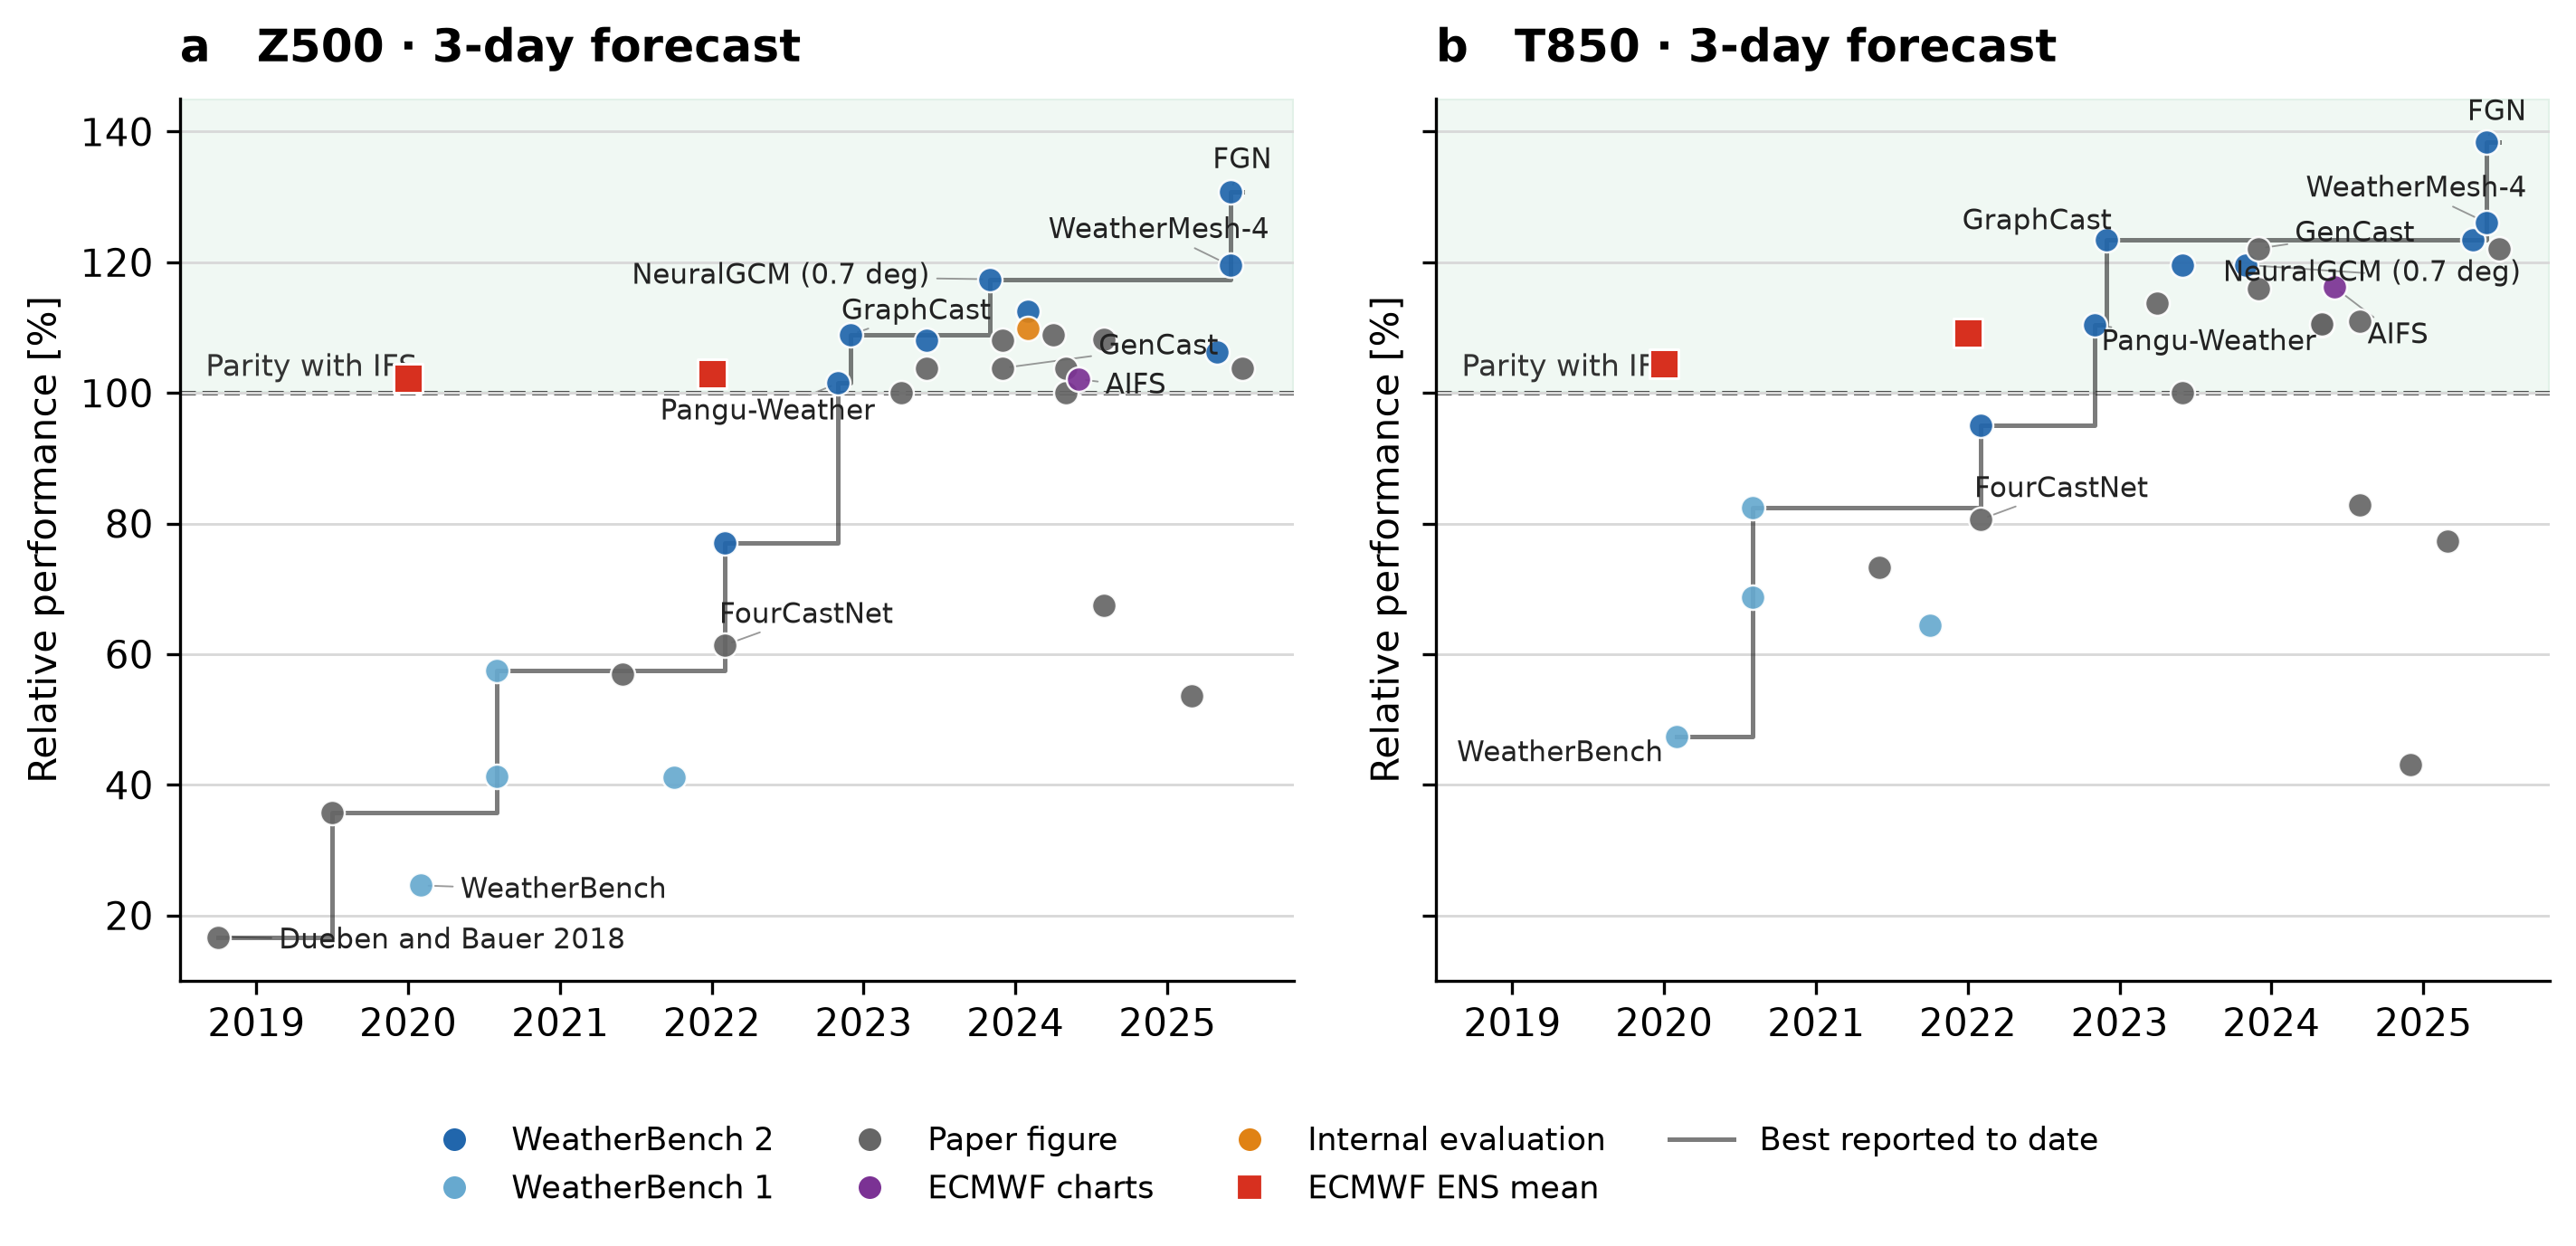
\includegraphics[width=1\linewidth]{Chapter1//figs/ai_weather_progress_relative.png}
    \caption{Evolution of global AI-based weather forecasting performance between 2018 and 2025 for three-day predictions of 500-hPa geopotential (Z500; left) and 850-hPa temperature (T850; right). Performance is expressed relative to the corresponding IFS reference as $100 \times \mathrm{RMSE}_{\mathrm{IFS}}/\mathrm{RMSE}_{\mathrm{model}}$; a value of 100 therefore indicates parity with IFS, while values above 100 indicate lower forecast error. The shaded region identifies models outperforming their IFS reference, and the step line shows the best reported performance up to each date. Colours distinguish the source of the evaluation, while red squares indicate the ECMWF ensemble mean. Because the results originate from heterogeneous evaluation periods, initial conditions, resolutions, and verification protocols, the figure illustrates the overall development of the field rather than providing a strict ranking of individual models. Data adapted from \citet{rasp2024aiweather}.}
    \label{fig:ai_weather_progress}
\end{figure}

AI models, however, are not limited to short- and medium-range weather forecasting. A distinct line of research aims to develop climate emulators capable of producing stable multidecadal simulations under prescribed boundary conditions and forcing scenarios, thereby moving towards capabilities traditionally associated with GCMs and ESMs. The emergence of such models has motivated the AI Model Intercomparison Project (AIMIP), which adapts the model-intercomparison philosophy of AMIP and CMIP to AI-based climate models \citep{henn_aimip_2026}. Initial AIMIP results indicate that these models can reproduce many features of the historical mean climate and atmospheric variability with skill comparable to a conventional numerical model, but also reveal model-dependent underestimation of observed warming trends and divergent responses under out-of-distribution warming scenarios.

Even if the capabilities of these models are already outstanding (Figure \ref{fig:ai_weather_progress}), realizing the potential of these models for Climate Services still requires overcoming both infrastructural and scientific challenges. From an infrastructural perspective, these models depend on specific training and inference methodologies, different requirements for their execution and formats for the input data. From a scientific perspective, their outputs require validation that extends beyond conventional measures of forecast accuracy. Statistical skill must be considered together with physical consistency, multivariate relationships, the representation of extremes, and robustness under conditions that differ from those included in the training data. In concrete, these means that the rapidly evolving and fragmented landscape of AI models for weather forecasting and climate simulation needs to be standardized into frameworks that can make their use reproducible, reliable, and robust.


\subsection{Diagnostic AI models}

Predictive models presented in the section above learn how atmospheric states evolve over time. Prediction, however, is only one way in which AI can operate on weather and climate data. A complementary application is diagnostic: rather than advancing the state of the atmosphere in time, machine learning methods identify coherent structures within observations, reanalyses, and climate simulations and transform them into climate information \citep{schneider_esa-ecmwf_2022}.

An important advantage of this approach is the possibility of constructing diagnostics that are more complex and more closely tailored to a specific scientific or operational purpose. Many conventional climate indices are defined through fixed thresholds, linear combinations, or a small number of variables. Although these indices remain transparent and physically interpretable, they may not fully represent phenomena arising from nonlinear, multivariate, and spatially heterogeneous interactions. Machine learning methods can instead combine multiple atmospheric, oceanic, and surface variables, account for their spatial and temporal dependencies, and learn specific mappings between physical conditions and quantities of interest. This makes it possible to derive data-driven indicators targeted for the most different uses \citep{molina_review_2023}.

The flexibility of diagnostic AI also introduces substantial methodological challenges. Model architectures must be able to represent multivariate spatio-temporal dependencies across different scales while preventing the algorithm from exploiting spurious correlations or dataset-specific features. Validation is particularly challenging because, unlike forecast verification, a unique ground truth may not exist for latent climate regimes or newly learned indicators. Evaluation should therefore combine conventional performance metrics, tests of physical consistency, and interpretability. 

 
\subsection{Large Language Models}

The methods discussed above transform numerical Earth System data into forecasts and climate descriptors. However, producing climate information does not by itself make it accessible, interpretable, or relevant to a particular decision context. A further challenge is to connect numerical outputs with the scientific, technical, and operational knowledge through which they acquire meaning, and to enable users to explore this heterogeneous information according to their specific questions.

Language is central to this process. Scientific findings are communicated through publications and reports, operational procedures are described in technical documentation, and user needs are expressed through questions, discussions, and descriptions of specific problems. Integrating the generalization capabilities of AI with language capabilities is one of the most impacting technological development of the last decades.

An important step in this direction was the development of methods for representing words as numerical vectors. Early neural language models learned both a representation of each word and the probability of observing it within a sequence \citep{bengio_neural_2003}. Later approaches such as Word2Vec made it possible to learn these representations efficiently from large textual collections \citep{mikolov_efficient_2013}. Words appearing in similar linguistic contexts tend to occupy similar positions in the resulting multidimensional space, allowing part of the syntactic and semantic structure of language to be represented in a form that can be processed by machine learning models.

A second major development was the introduction of the Transformer architecture \citep{vaswani_attention_2017}. Its central mechanism, known as \textit{self-attention}, allows the representation of each element of a text to be constructed by considering its relationships with the other elements in the sequence. The meaning assigned to a word can therefore depend on the surrounding context rather than on the word in isolation. Moreover, unlike recurrent architectures, Transformers can process different positions of a sequence in parallel during training. Combined with increasingly large textual datasets and computational resources, this property enabled the training of models with a rapidly growing number of parameters.

Large Language Models (LLMs) are high-capacity neural language models, generally based on the Transformer architecture, trained on extensive and heterogeneous textual corpora. They process text by dividing it into elementary units called \textit{tokens}, which may correspond to entire words, parts of words, punctuation marks, or individual characters. In an autoregressive LLM, the model estimates the probability of the next token on the basis of the preceding sequence. During generation, a token is selected from the predicted probability distribution and appended to the sequence. The updated sequence is then used to predict the following token, and the process is repeated iteratively. 

Following the introduction of the Transformer, the development of LLMs accelerated through a combination of model scaling, post-training, and broader accessibility. GPT-3 demonstrated that increasing model and dataset size could produce strong zero- and few-shot performance, allowing a single pretrained model to address previously unseen tasks from instructions or examples provided directly in its input context \citep{brown_language_2020}. Instruction tuning and reinforcement learning from human feedback subsequently transformed pretrained language models into systems better able to follow user requests, as demonstrated by InstructGPT \citep{ouyang_training_2022}. GPT-4 extended this trajectory through improved performance across academic and professional benchmarks and the integration of textual and visual inputs \citep{openai_gpt-4_2023}, while open-weight model families such as Llama 2 made high-capacity pretrained and dialogue-optimized models more accessible to the broader research community \citep{touvron_llama_2023}. More recently, reasoning-oriented models have combined multi-stage post-training and reinforcement learning to improve performance on tasks requiring extended intermediate reasoning \citep{deepseek-ai_deepseek-r1_2025}. The rapid progression resulting from these developments is illustrated in Figure~\ref{fig:llm_benchmark_progress}.

\begin{figure}[H]
    \centering
    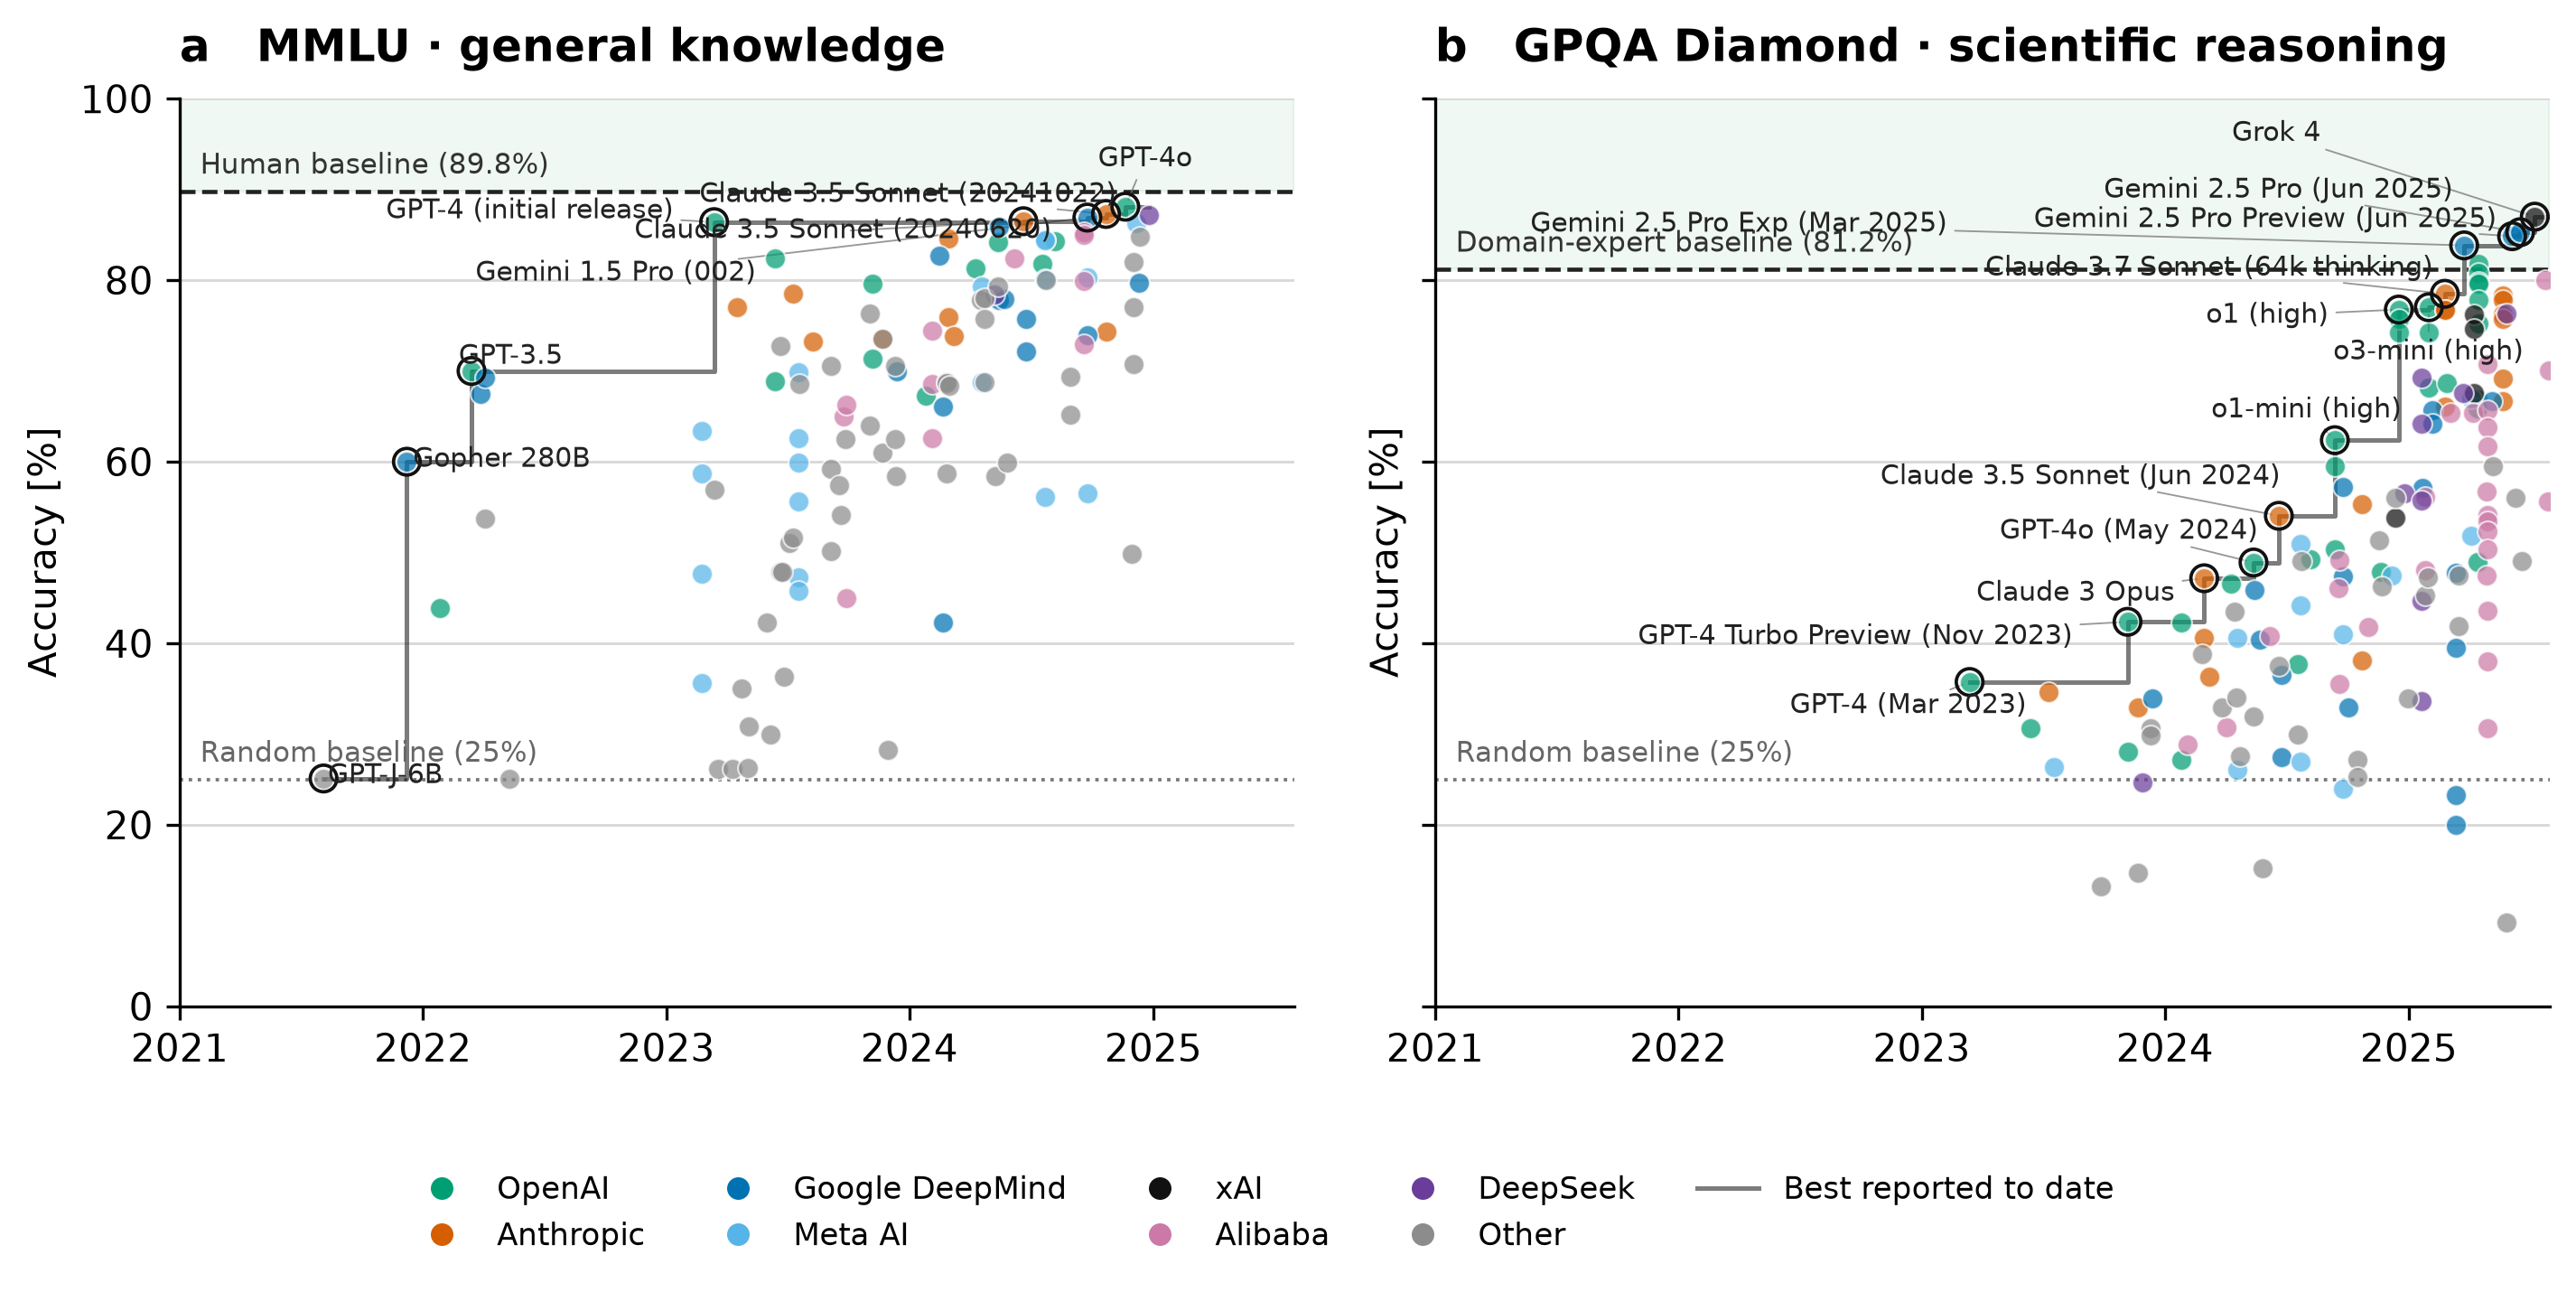
\includegraphics[width=1\linewidth]{Chapter1/figs/llm_benchmark_progress.png}
    \caption{Evolution of Large Language Model performance on MMLU and GPQA Diamond through July 2025. MMLU evaluates broad academic and professional knowledge across 57 subjects \citep{hendrycks2021mmlu}, whereas GPQA Diamond comprises graduate-level questions in biology, chemistry, and physics selected for their difficulty and expert-validated answers \citep{rein2024gpqa}. Each point represents a model evaluation and colours identify the developing organization. Black-outlined markers indicate models that established a new performance frontier, while the step line shows the best reported accuracy available at each date. The dotted line represents random-guessing accuracy (25\%), and the dashed lines show the reported human reference levels: 89.8\% for MMLU \citep{maslej2025aiindex} and 81.2\% for GPQA Diamond \citep{rein2024gpqa}. The shaded regions identify scores above these human references. MMLU results are restricted to five-shot evaluations, while GPQA Diamond values correspond to mean scores reported by the Epoch AI benchmarking framework \citep{epoch2026benchmarking}. Since MMLU results originate from heterogeneous external evaluations that may differ in prompting and implementation details, the figure illustrates the overall progression of benchmark performance rather than providing a strict ranking of individual models.}
\label{fig:llm_benchmark_progress}
\end{figure}

As their scale has increased, LLMs have consequently shown the ability to perform a broad range of tasks through the same linguistic interface, including summarizing documents, extracting relevant information, connecting concepts, and adapting explanations to different questions or audiences \citep{li_fundamental_2024}. The ability to perform different tasks through the same linguistic interface positions LLMs not merely as text generation systems, but as potential interfaces to information. A potential application concerns the fact that the same general-purpose technology can provide meaningful access to the heterogeneous knowledge base underpinning Climate Services. This knowledge is distributed across scientific papers, institutional and technical reports produced for different purposes and audiences, numerical climate datasets, geospatial information, and climate-model outputs. A natural language interface may reduce the technical effort required to formulate a query, access information, and produce tailored knowledge. 

But the versatility and power of LLMs generative capabilities also raises fundamental questions on how their output can be evaluated, both in terms of factual accuracy and epistemic quality for Climate Services purposes.  


%*******************************************************************************
%**************** Third Section - Research framework and thesis outline ********
%*******************************************************************************
\section{Research framework and thesis outline}

The previous sections introduced the operational framework of Climate Services and the main Artificial Intelligence paradigms examined in this thesis. This section brings the two fields together and positions the research contributions along the Climate Services value chain. The central research question is how AI can improve both the production of climate information and its transformation into accessible, specific, and relevant knowledge, and how its outputs should be evaluated to ensure that they remain scientifically reliable. 

As seen in the previous sections, AI is a broad and highly heterogeneous field, encompassing a wide range of concepts, methods, and algorithms. A comprehensive review of its potential applications is therefore beyond the scope of this dissertation. Instead, this thesis adopts a selective approach. It examines a set of representative AI applications positioned at different stages of the Climate Services value chain, from the production of climate data to their transformation into information and decision-relevant knowledge. Rather than attempting to catalogue all possible uses of AI, the thesis investigates the opportunities offered by selected AI paradigms and the methodological requirements needed to integrate them into scientifically robust and operationally useful Climate Services.

Against this background, the following chapters present the research contributions through the methodological frameworks, use cases, and evaluation approaches developed during the research period:

\begin{itemize}

\item Chapter~2 introduces AIUQ, a framework developed in collaboration with the Barcelona Supercomputing Center. AIUQ standardizes the inference workflow of AI-based weather forecasting models, reducing the operational complexity involved in producing large ensembles of simulations with heterogeneous models. It also introduces an evaluation framework for testing their out-of-sample behavior and assessing their ability to generalize across configurations and climatic conditions that differ from those encountered during training. This chapter addresses the first step of the Climate Services value chain: the reliable, robust, and reproducible production of climate data through AI.

\item Chapter~3 moves from prediction to diagnosis by introducing a machine-learning framework for deriving objective, data-driven definitions of meteorological seasons from reanalysis data and applying them consistently to climate-model projections. The framework is applied to the Indian subcontinent, where seasonality has major societal and economic implications because of the monsoon and where the extensive scientific knowledge available provides a strong basis for validating the proposed approach. This chapter addresses the second step of the Climate Services value chain: the transformation of climate data into information through AI, while examining the practical advantages of data-driven algorithms over deterministic definitions.

\item Chapter~4 introduces the contribution of Large Language Models to Climate Services by addressing a first fundamental evaluation question: to what extent do LLMs encode reliable climate information in their parametric knowledge? To answer this question, a practical benchmark for assessing the climate knowledge of different LLMs was developed at the Alfred Wegener Institute and applied to a selection of open-source and proprietary models. Within the Climate Services value chain, this chapter examines the capacity of LLMs to retrieve, connect, and communicate information as a basis for knowledge creation.

\item Chapter~5 addresses a second fundamental question: how can the epistemic quality of LLM outputs be evaluated in the context of Climate Services? The chapter introduces a framework that assesses answers to climate-related questions along four dimensions: relevance, actionability, credibility, and uncertainty communication. The framework is then applied to four LLM-based systems implementing different augmentation strategies and interacting with different sources of climate knowledge: textual information retrieval, operations on numerical climate data, and combinations of the two. This chapter addresses the transition from information to knowledge by examining how LLMs can contextualize heterogeneous climate content while preserving the qualities required for its use in Climate Services.

\end{itemize}

Figure~\ref{fig:research_framework} summarizes the relationship between the operational framework of Climate Services and the contributions of the thesis.

\begin{figure}[H]
\centering
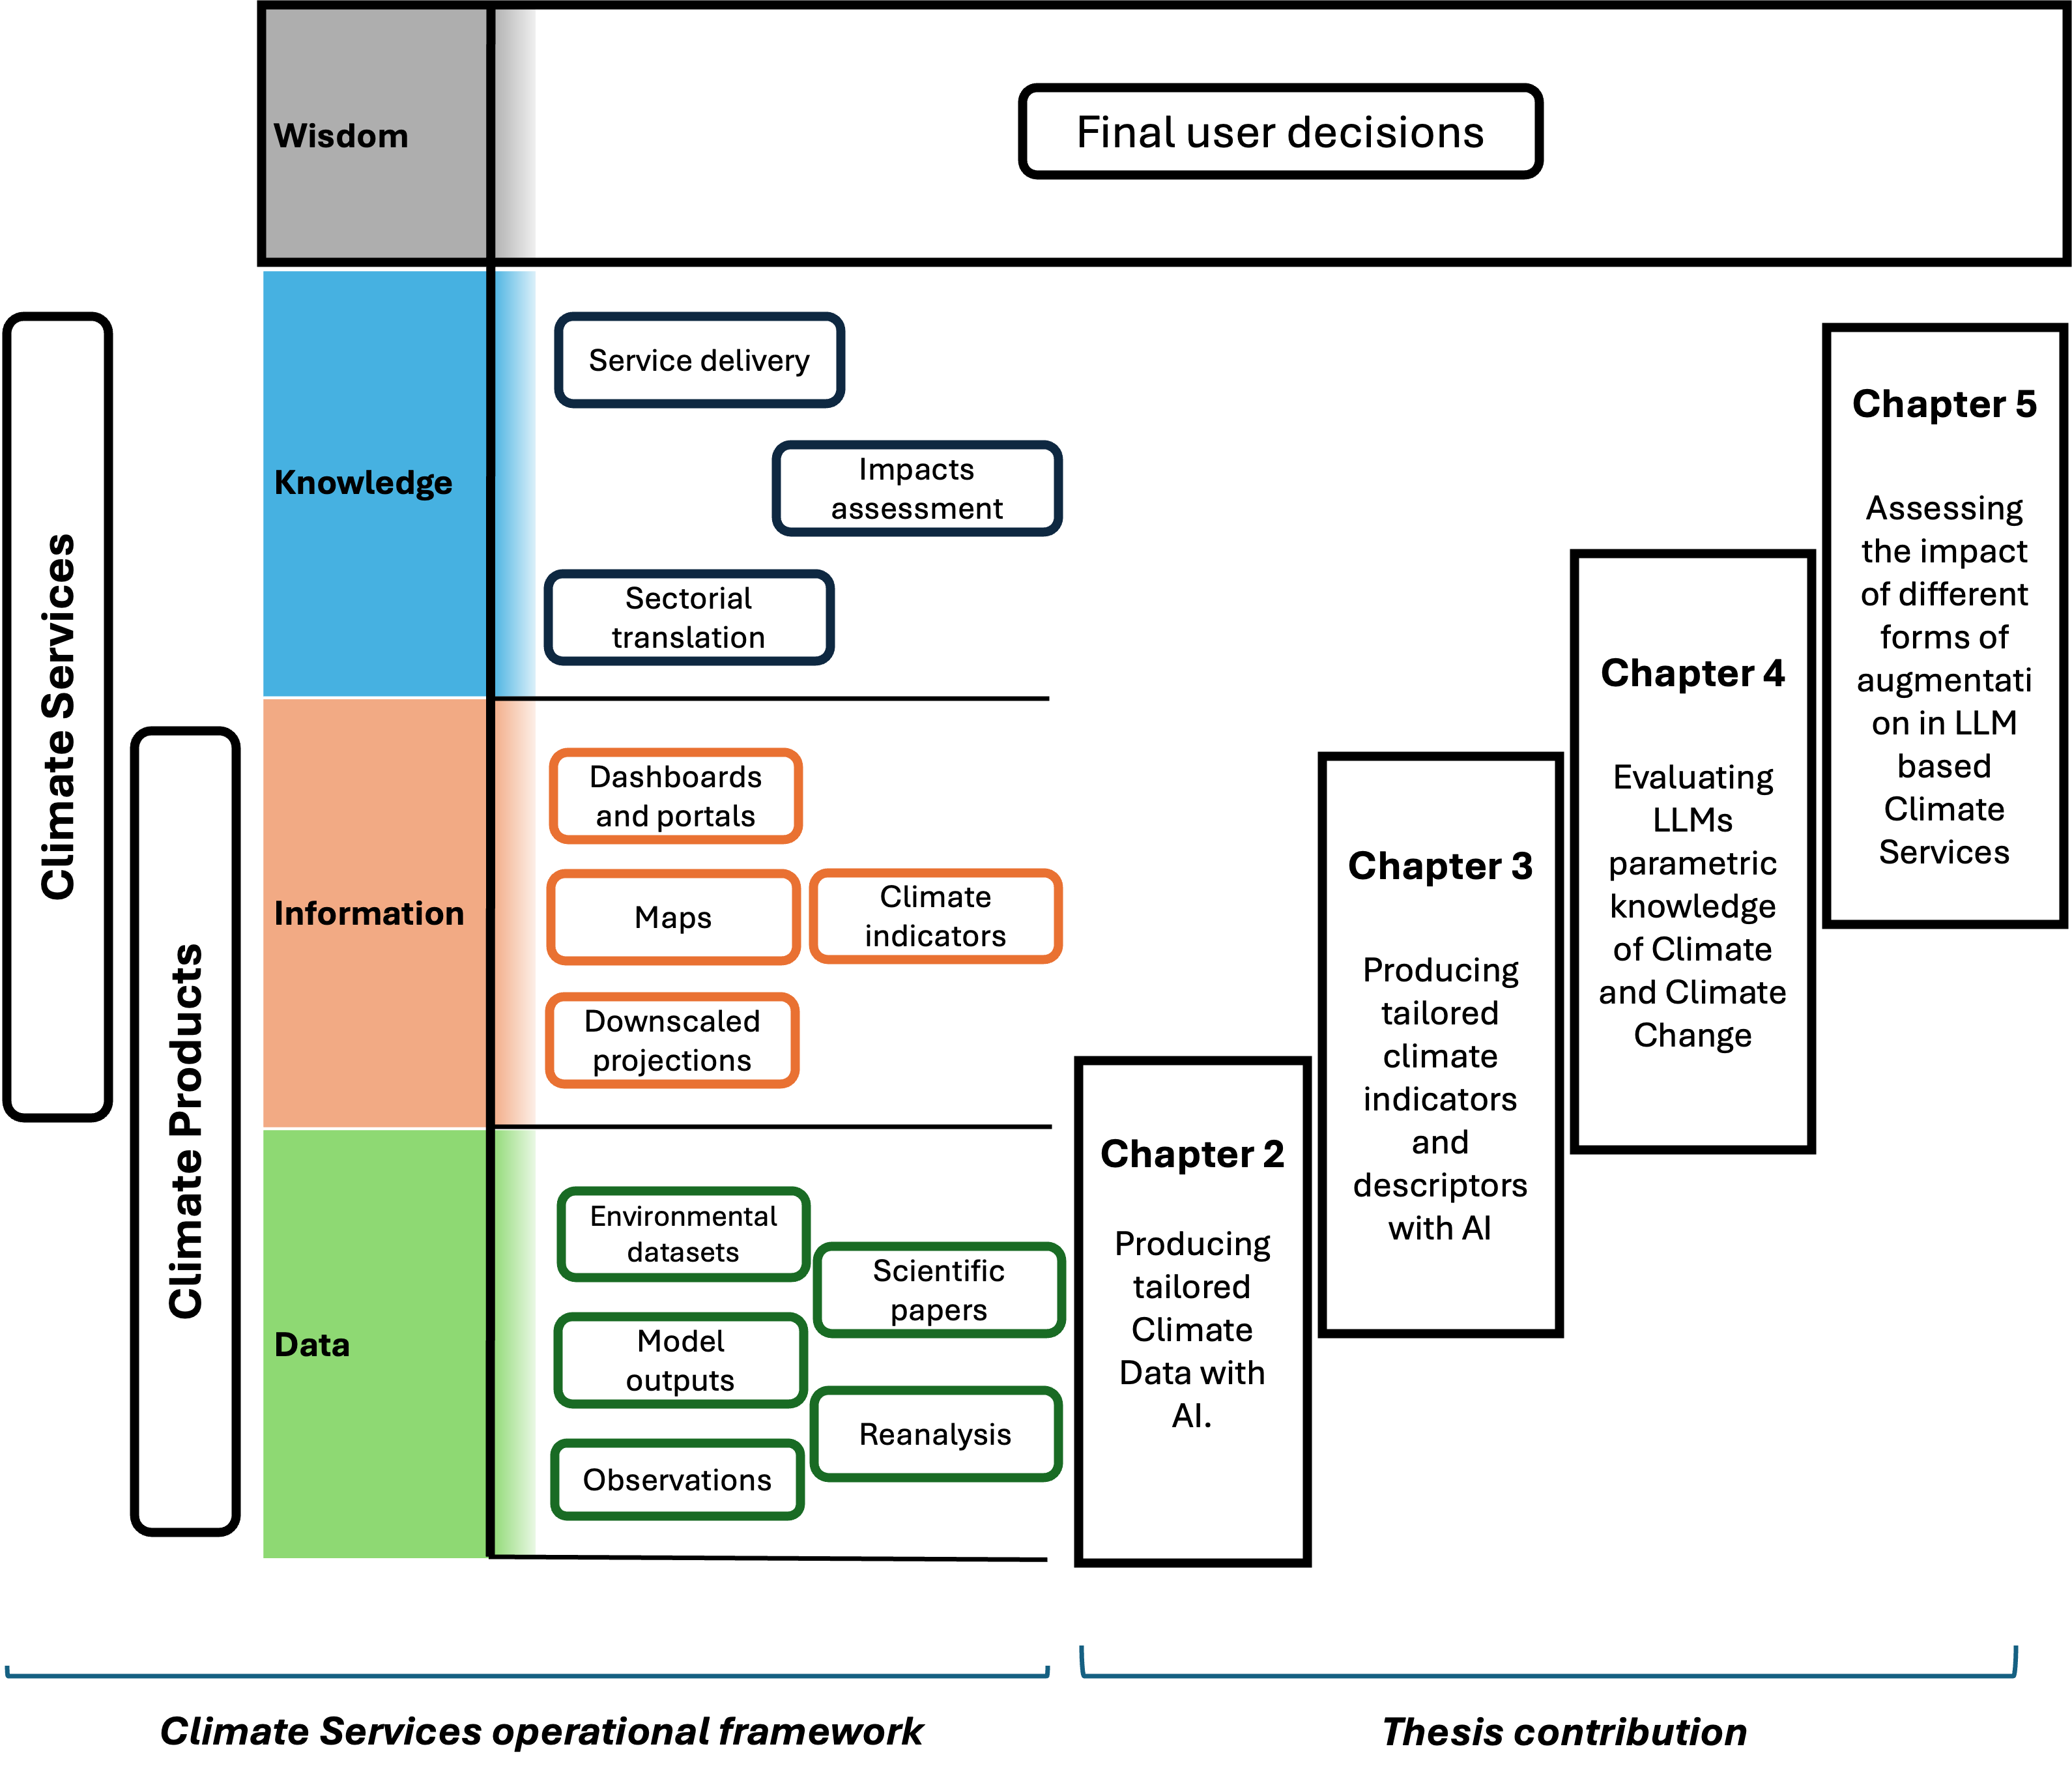
\includegraphics[width=\linewidth]{Chapter1/figs/framework.png}
\caption{Conceptual framework linking the operational structure of Climate Services to the contributions of this thesis. The left-hand panel represents the progression from heterogeneous climate data to information, knowledge, and ultimately decision-relevant wisdom, while distinguishing Climate Products from the broader Climate Services through which these products are interpreted and connected to their use. The right-hand panel positions Chapters~2--5 within this progression.}
\label{fig:research_framework}
\end{figure}


\chapter{Reliable Data with AI Weather Models}

% **************************** Define Graphics Path **************************
\ifpdf
    \graphicspath{{Chapter3/Figs/}{Chapter3/Figs/PDF/}{Chapter3/Figs/}}
\else
    \graphicspath{{Chapter3/Figs/Vector/}{Chapter3/Figs/}}
\fi

\noindent\textit{The research presented in this chapter was the final component of the dissertation to be undertaken and, unlike the work described in the subsequent chapters, has not yet been the subject of a dedicated journal publication. Its two components are currently at different stages of consolidation. The software framework for running AI weather models on high-performance computing systems was developed at the Barcelona Supercomputing Center and has already supported other research applications. The scientific validation framework is more recent and should therefore be regarded as an initial methodological contribution whose further development and testing are still ongoing. Nevertheless, the chapter is presented first because it addresses the production of climate data and thus provides the logical starting point for the progression developed throughout the dissertation.}

\vspace{0.5em}
\begin{center}
    \rule{0.5\textwidth}{0.4pt}
\end{center}
\vspace{0.5em}


In 1974, \citet{schneider_climate_1974} described the development of climate models as a means ``first to derive better understanding and ultimately to allow some degree of predictive capability.'' Their review connected this scientific ambition to pressing societal concerns, including climate-related food shortages and the possibility that human activities could alter the climate. The prospect was that a quantitative representation of the climate system could eventually help societies anticipate changes whose consequences extended beyond atmospheric science.

Over the following decades, advances in physical understanding, numerical methods, observations, and computing transformed this prospect into an established scientific capability. Climate models developed into coupled representations of the atmosphere, ocean, land surface, and cryosphere, with Earth System Models incorporating additional biogeochemical processes. Coordinated experiments now provide projections of climate change under different forcing scenarios \citep{eyring_overview_2016}. Combined with models of exposed natural and human systems, these simulations support assessments of climate impacts across sectors and geographical scales \citep{huber_climate_2014}. Climate modelling has therefore become a foundation for investigating future risks and producing the data on which many Climate Services depend.

Over the last few years, Artificial Intelligence has introduced new approaches to simulating weather and climate. Models trained on atmospheric reanalyses can now generate global weather forecasts with skill comparable to, and for many evaluated variables exceeding, that of established numerical forecasting systems. These developments encompass a range of architectures and training strategies, from fully data-driven forecasting systems to the integration of learned components into physical models \citep{de_burgh-day_machine_2023}. In parallel, climate emulators have been developed to reproduce atmospheric evolution and climate statistics at substantially lower computational cost. For example, ACE2 can generate stable multi-decadal atmospheric simulations and reproduce historical variability and temperature trends under prescribed boundary conditions and forcings \citep{watt-meyer_ace2_2025}. These developments open opportunities for producing larger ensembles and exploring atmospheric variability more extensively. 

Despite their rapid progress, the suitability of AI weather and climate models for Climate Services cannot be established from aggregate forecast scores alone. Evaluation must also consider the representation of extremes, consistency between variables, and climatic variability \citep{schultz_can_2021}. In deterministic forecasting, minimizing mean squared error can favour increasingly smooth predictions as uncertainty grows \citep{lang_aifs-crps_2026}. Moreover, \citet{sun_can_2025} showed that versions of FourCastNet with similar global verification scores differed substantially in their ability to predict intense tropical cyclones absent from their training data.

The development of these models also depends on the quality and availability of their training data. Many leading systems rely on reanalyses such as ERA5, which combine observations and numerical forecasts through data assimilation \citep{hersbach_era5_2020}. Continued investment in observations, physical modelling, and reanalysis production therefore remains important, alongside emerging approaches trained directly on observations \citep{mcnally_data_2024}. This dependence also creates a risk of inheriting systematic errors: global coverage does not imply uniform data quality, and agreement with a training reference does not guarantee equivalent agreement with independent observations. As argued by \citet{mozaffari_rise_2026}, uneven data quality and unequal access to computational infrastructure can also concentrate the benefits of AI. 

These considerations motivate a more systematic approach to executing and evaluating AI weather models for climate applications. The evaluations accompanying new model releases provide essential evidence of their capabilities, but their conclusions remain conditional on the selected datasets, initialization procedures, forecast horizons, and verification criteria. Establishing their suitability for Climate Services requires extending these assessments to additional experimental configurations, including initialization from climate simulations and the evaluation of climatic statistics beyond conventional forecast skill.

Shared inference tools, including ECMWF's \emph{ai-models}\footnote{An open-source Python package providing a common command-line interface for running AI weather models through model-specific plugins, with support for retrieving initial conditions and managing forecast outputs. See \url{https://github.com/ecmwf-lab/ai-models}.} and NVIDIA's Earth2Studio\footnote{An open-source Python framework offering a unified interface and modular components for constructing AI weather and climate inference workflows, including data sources, pretrained models, ensemble generation, and output handling. See \url{https://nvidia.github.io/earth2studio/}.}, have reduced the technical barriers to running different models, while WeatherBench~2 provides a common framework for forecast verification \citep{rasp_weatherbench_2024}. Building on these developments, a further requirement is to connect data preparation, ensemble execution, output harmonization, and scientific evaluation within reproducible experiments. This becomes particularly relevant when comparing models initialized from heterogeneous datasets, managing many initialization dates and ensemble members, and examining how their behaviour changes with forecast lead time.

This chapter addresses this requirement through two complementary contributions. The first is AIUQ, a modular workflow developed at the Barcelona Supercomputing Center to coordinate the execution of AI weather models on high-performance computing systems. Its common data representation separates the preparation of initial conditions from model-specific inference, facilitating experiments across different models and data sources. The second is an initial evaluation of forecasts generated from climate model outputs, examining ensemble forecast skill, climatological agreement, stability, and anomaly amplitude. These contributions address the first stage of the Climate Services value chain: determining under which conditions AI models can support the production of reliable climate data.

\section{Methods}

\subsection{AIUQ Workflow} \label{workflow}

AIUQ is organized as a modular workflow in which orchestration, data preparation, model execution, and output harmonization are separate concerns. The workflow is coordinated by Autosubmit \citep{manubens-gil_seamless_2016}, while the scientific transformations are implemented by source- and model-specific adapters. At the centre of the architecture is the AIUQ standard, which acts as a data contract between initial-condition (IC) sources and forecasting models. Consequently, an IC source only needs to produce the standard representation and a model only needs to consume it; no dedicated interface is required for every source--model pair. Figure~\ref{fig:aiuq-pipeline} summarizes the resulting pipeline.

\begin{figure}[H]
    \centering
    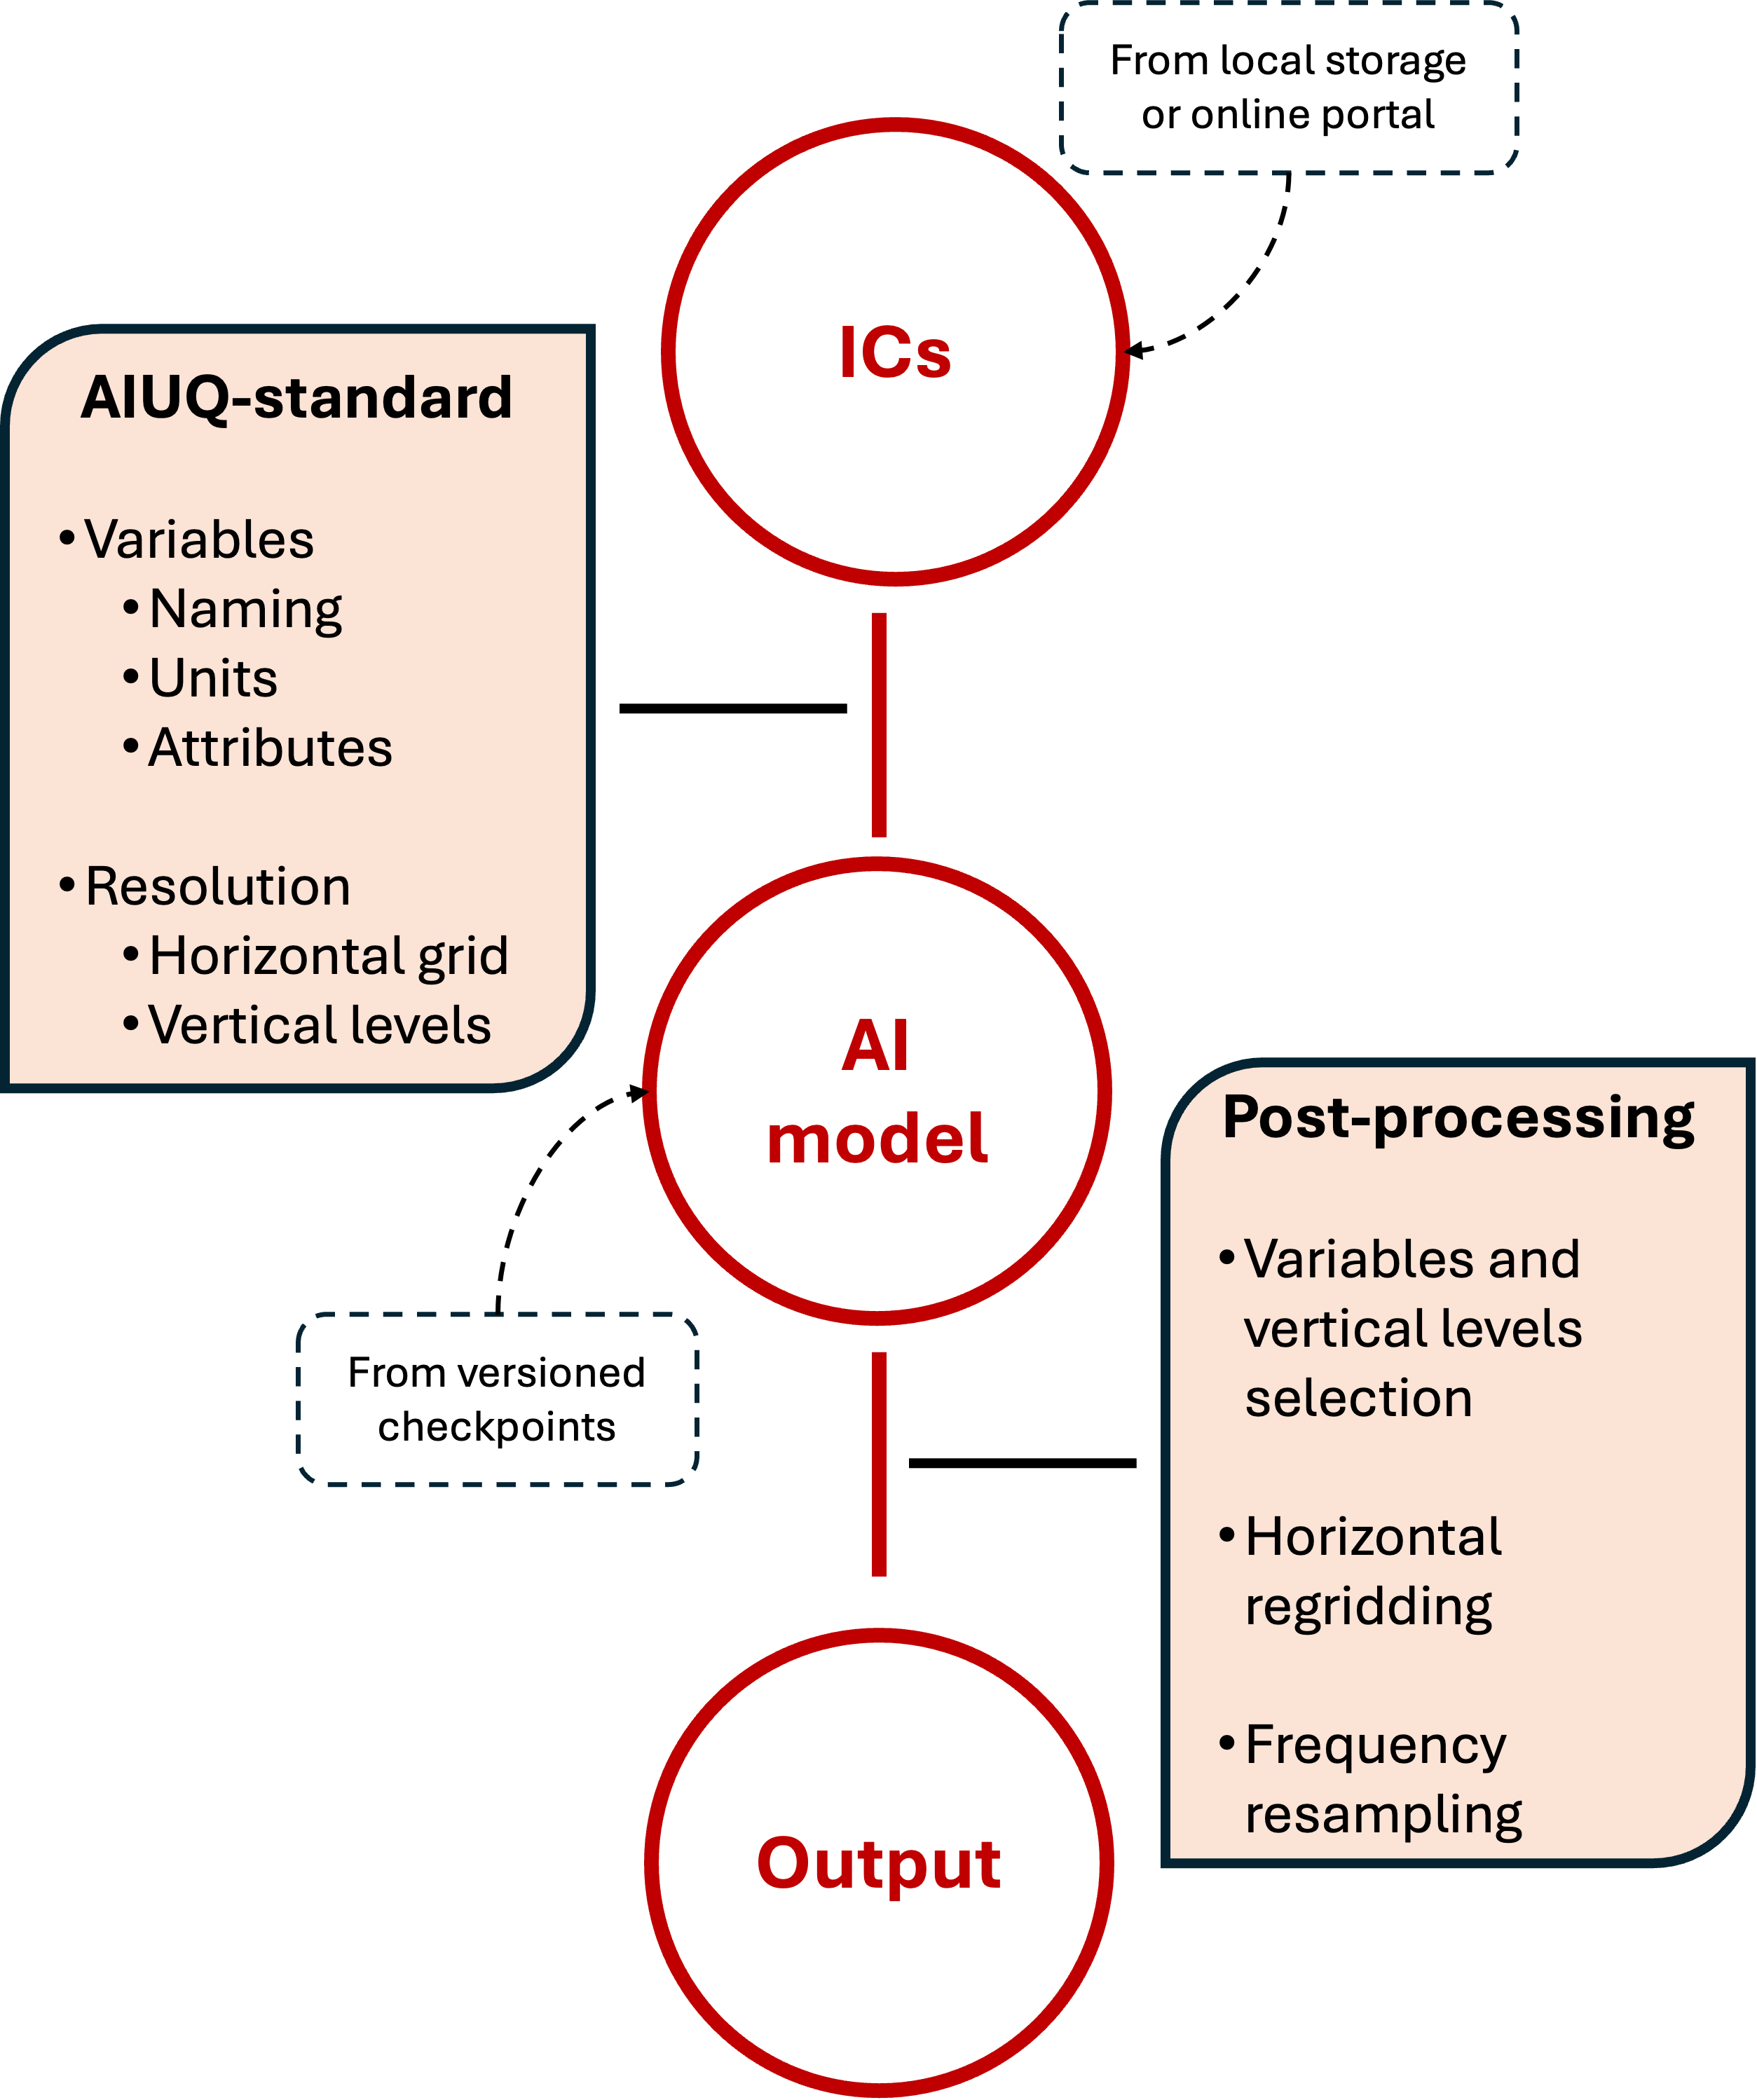
\includegraphics[width=0.55\linewidth]{Chapter2/Figs/aiuq-pipeline.png}
    \caption{Overview of the AIUQ workflow. Source-specific adapters retrieve or read ICs and normalize them to the AIUQ standard. Model-specific adapters translate this common representation to the requirements of the selected checkpoint, while the post-processing stage harmonizes the requested forecast outputs.}
    \label{fig:aiuq-pipeline}
\end{figure}

\paragraph{Configuration} \label{configuration}

An AIUQ experiment is defined declaratively through YAML configuration files. The user selects the forecasting model and checkpoint, the IC source, the initialization dates, the ensemble members, and the temporal chunking of the simulation. The same configuration also describes the requested output variables, pressure levels, temporal frequency, and horizontal resolution. Platform-specific options specify where each task is executed and which computational resources it requires, together with the paths to auxiliary files needed for the execution. At submission time, Autosubmit constructs the experiment graph, combining the specific jobs for the retrieval and preparation of the ICs and for running the inference with the AI models.  

\paragraph{ICs preparation} \label{ics-preparation}

The ICs preparation stage converts heterogeneous input data into a source independent representation. A source adapter either retrieves the requested fields from an online archive or reads them from local storage. Each source is described by an IC card containing its variable names, identifiers, vertical coordinates, and access-specific metadata. These entries are matched against the selected version of the AIUQ standard, after which the retrieved dataset is subset, renamed, and assigned the common coordinates and attributes. Pressure levels and horizontal coordinates are harmonized when necessary. If the primary source does not provide all fields required by the standard, AIUQ invokes the configured fallback hierarchy. 

\paragraph{Fallbacks} \label{fallbacks}
An IC source may not provide every field defined by the AIUQ standard. During IC preparation, AIUQ compares the variable identifiers declared in the source card with those required by the selected standard version. To fill the gaps AIUQ applies a deterministic fallback hierarchy. Missing time-invariant surface fields are first obtained from a shared static dataset; these include orography, the land--sea mask, and descriptors of sub-grid-scale orography obtained from ECMWF. Fields that remain unavailable can then be supplied from a climatological dataset obtained from ERA5. 

\paragraph{Model inference} \label{model-inference}

At the inference stage, the model chosen in the configuration is fed with the ICs prepared at the stage before. A model card maps AIUQ standard to the specific input expected by the model. The adapter then performs only the transformations intrinsic to that backend, such as selecting fields, interpolating to the model grid, changing array layout, or constructing the model's native input state. Inference is executed inside a model-specific container using a versioned checkpoint stored outside the workflow repository. For stochastic models, the ensemble member identifier is also used to initialize the model, making individual realizations reproducible. Model states can be checkpointed where supported, so long integrations such as climate scale simulations can be divided into manageable segments and resumed after interruptions.

\paragraph{Post-processing} \label{post-processing}

The final stage transforms native forecasts into standardized output. AIUQ retains only the variables and vertical levels requested by the user, translates model specific names back to the common convention, and applies the selected temporal aggregation and horizontal regridding. This design avoids storing the full native output when only a subset is needed and makes the computational and storage cost of an experiment configurable. Processed fields are written as NetCDF files organized by variable, ensemble member, and forecast interval, with consistent temporal and spatial coordinates. The resulting simulations therefore share a predictable layout across models and IC sources and can be compared directly or passed to downstream components.


\subsection{Experiment configuration} \label{experiment-configuration}

This study uses ERA5 and the EERIE-AMIP simulations, both representing historical climate conditions. ERA5 \citep{hersbach_era5_2020} is a widely used global reanalysis that combines historical observations with a numerical weather prediction model through data assimilation, providing a reconstruction of past atmospheric conditions. The dataset currently covers the period from 1940 to the present \citep{soci_era5_2024}. ERA5 is extensively used to train AI weather models and serves as a common reference for evaluating their forecasts. Initializing and verifying these models against ERA5 therefore provides a reference configuration closely aligned with their training data in terms of data source. We regard this as an approximately in-distribution setting, without assuming that the training and evaluation distributions are identical. ERA5 fields were retrieved from the public Analysis-Ready, Cloud-Optimized (ARCO) archive hosted on Google Cloud Storage \citep{carver_arco-era5_2023}.

The EERIE-AMIP simulations \citep{aengenheyster_multi-decadal_2026} were produced at ECMWF using an atmosphere-only configuration of the Integrated Forecasting System (IFS), covering 1980--2023. Initialized from ERA5 in January 1980, the simulations evolve freely without atmospheric data assimilation, with prescribed sea surface temperatures, sea ice concentrations, and external radiative forcings. They therefore generate their own weather trajectories rather than reconstructing the observed sequence of weather events. Their climatology is expected to broadly resemble the observed historical climate, although systematic model biases remain. Although ERA5 and EERIE-AMIP both use the IFS, they differ in model configuration and observational constraints. Initializing and verifying AI forecasts against EERIE-AMIP thus provides a potentially out-of-distribution setting, testing generalization to model-generated atmospheric states under broadly comparable historical climate conditions. EERIE-AMIP fields were retrieved through ECMWF's Meteorological Archival and Retrieval System (MARS).

We used two AI-based global weather forecasting models, NeuralGCM and AIFS-CRPS. NeuralGCM \citep{kochkov_neural_2024} combines a differentiable atmospheric dynamical core with neural networks that represent unresolved physical processes, such as cloud formation, radiation, and convection. The model is trained end-to-end on ERA5 trajectories and supports both deterministic and stochastic configurations. In the stochastic configuration, spatially and temporally correlated noise is incorporated into the learned parameterizations, enabling ensemble forecasting. In the original evaluation, the stochastic model at approximately $1.4^\circ$ resolution achieved lower ensemble-mean RMSE and CRPS than the operational ECMWF ensemble for most evaluated variables and lead times up to 15 days. Separate deterministic configurations also reproduced key climate statistics in multi-year to multi-decadal simulations with prescribed sea surface temperature and sea ice.

AIFS-CRPS \citep{lang_aifs-crps_2026} is a probabilistic forecasting model developed at ECMWF. Its encoder--processor--decoder architecture combines an attention mechanisms with a transformer processor and advances the atmospheric state in six-hour steps. The model is trained on ERA5, with operational IFS analyses used for additional training of the medium-range configurations. Ensemble members are generated through stochastic noise injected into the network, while an almost fair CRPS training objective jointly rewards forecast accuracy and appropriate ensemble spread. Published evaluations showed improved CRPS relative to the physics-based IFS ensemble for most variables and lead times up to 15 days. Experiments with a lower-resolution configuration also demonstrated competitive skill for weekly anomalies in 46-day forecasts, extending its potential applications to subseasonal prediction.

For both AI models, 10-member ensemble forecasts were initialized every 10 days during 1985--1990 using atmospheric states from EERIE-AMIP member 1, with each forecast extending to 30 days. The full 10 members EERIE-AMIP ensemble and ERA5 were used as comparison datasets. During post-processing, all datasets were regridded to a common regular latitude--longitude grid with a spacing of $1^\circ \times 1^\circ$ and aggregated into daily means. The analysis focused on temperature at 850 hPa.

\subsection{Evaluation criteria}
\label{evaluation}

The evaluation addresses two complementary aspects of model performance: the accuracy of ensemble forecasts in predicting the evolution of individual weather trajectories, and their ability to reproduce the climatological mean fields of the reference datasets. Forecast accuracy is assessed using the Continuous Ranked Probability Score (CRPS), while climatological agreement is evaluated through global mean bias and spatial root mean square error (RMSE). All metrics are calculated on the common verification grid. Spatial averages are weighted on the cosine of the latitude:

\begin{equation}
    w_i = \frac{A_i}{\sum_{j=1}^{N} A_j},
\end{equation}

where $A_i$ is the area of grid cell $i$ and $N$ is the number of grid cells.

\paragraph{Ensemble forecast accuracy}

The CRPS evaluates a predictive distribution against a verifying value \citep{gneiting_strictly_2007}. For a forecast cumulative distribution function $F$ and a reference value $r$, it is defined as
\begin{equation}
    \mathrm{CRPS}(F,r)
    =
    \int_{-\infty}^{+\infty}
    \left[F(x)-H(x-r)\right]^2 \,\mathrm{d}x,
    \label{eq:crps}
\end{equation}
where $H(x-r)$ is the Heaviside step function, equal to zero for $x<r$ and one for $x\geq r$. For an ensemble of $M$ equally weighted members with predicted values $x_1,\ldots,x_M$, the CRPS of the empirical forecast distribution can equivalently be written as
\begin{equation}
    \mathrm{CRPS}(F,r)
    =
    \frac{1}{M}\sum_{k=1}^{M}|x_k-r|
    -
    \frac{1}{2M^2}
    \sum_{k=1}^{M}\sum_{j=1}^{M}|x_k-x_j|.
    \label{eq:crps-ensemble}
\end{equation}
The score accounts for both the location and spread of the forecast distribution. Lower values indicate better performance, and the score has the same physical units as the evaluated variable. For a deterministic forecast, it reduces to the absolute error.

For the EERIE-initialized experiments, the verifying values are taken from the evolving EERIE-AMIP member~1 trajectory, which also supplies the initial conditions. This comparison therefore evaluates the ability of the AI models to predict the subsequent evolution of the source simulation. The CRPS is calculated locally before spatial averaging with the weights $w_i$, and the resulting global scores are averaged across initialization dates at each lead time.

\paragraph{Climatological agreement}

Daily climatologies are constructed for each day of the year over the study period, with forecast values assigned according to their valid date. These climatologies also retain information about forecast lead time, defined as the time elapsed since initialization. At short lead times, the predicted atmospheric states remain closely tied to the initial conditions and therefore to the source dataset. As lead time increases, this influence gradually weakens, and the forecasts increasingly reflect each AI model's own dynamics and systematic tendencies. Retaining the lead-time dimension therefore allows us to examine how the model climatology evolves during the forecast and whether it progressively departs from that of the initialization dataset.

Climatological differences are evaluated using the area-weighted global mean bias and spatial RMSE. The bias indicates whether the model overestimates or underestimates the reference global mean:

$$
\mathrm{Bias}
=
\sum_{i=1}^{N} w_i
\left(\overline{X}^{A}_{i}-\overline{X}^{R}_{i}\right)
$$

The RMSE measures the magnitude of spatial differences, capturing regional errors that may cancel in the global mean:

\begin{equation}
    \mathrm{RMSE}
    =
    \sqrt{
    \sum_{i=1}^{N} w_i
    \left(\overline{X}^{A}_{i}-\overline{X}^{R}_{i}\right)^2
    } 
\end{equation}

\paragraph{Anomaly amplitude}

The amplitude of daily temperature anomalies is examined as an additional diagnostic of model behaviour. Related measures, often referred to as forecast activity, have been used to assess the magnitude of departures from climatology in AI weather forecasts. Monitoring their evolution with lead time is relevant for identifying changes in atmospheric variability, including the damping or artificial amplification of forecast structures \citep{lang_aifs-crps_2026}.

Daily temperature anomalies are calculated relative to each dataset's own day-of-year climatology over 1985--1990, using the forecast valid date to select the corresponding climatological field. For each initialization, their spatial root mean square is calculated as

\begin{equation}
    \mathrm{RMS}(t)
    =
    \sqrt{
        \sum_{i=1}^{N} w_i
        \left[T'_i(t)\right]^2
    }.
    \label{eq:anomaly-rms}
\end{equation}

where $T'(t)$ denotes the daily temperature anomaly and
$\langle \cdot \rangle_{\mathrm{space}}$ denotes spatial averaging over the global domain.

The resulting curves are examined as a function of forecast lead time and compared with EERIE-AMIP over the corresponding dates. This comparison assesses whether the models maintain comparable anomaly amplitudes as the forecasts progress. 


\section{Results}

\subsection{Computational performance and forecast stability}
\label{sec:performance-stability}

The initial assessment examines the computational feasibility of the experiment and the behaviour of the forecasts over the 30-day integration period. Selected forecasts initialized in 1987 illustrate the main features.

Figure~\ref{fig:example-inference-maps} compares the ensemble-mean temperature at 850~hPa from both AI models with the corresponding EERIE-AMIP member~1 field, ten days after initialization. Both models retain the broad geographical distribution of temperature, including the meridional gradient and the main continental thermal contrasts. Their ensemble means are smoother than the individual EERIE-AMIP realization, consistent with averaging members whose weather patterns progressively diverge. Substantial regional differences nevertheless emerge. The bias patterns of the two models are notably similar, with a spatial correlation coefficient of approximately $r=0.85$ in this example.

The global mean temperature provides a complementary view of forecast evolution (Figure~\ref{fig:global-temperature}). For the three initialization dates shown, AIFS-CRPS develops a recurring cooling tendency during the latter part of the integration, beginning around days 15--20. This behaviour is particularly pronounced in summer (Figure~\ref{fig:global-temperature-summer}), suggesting a forecast drift whose magnitude depends on season and lead time. NeuralGCM does not exhibit the same late-stage cooling in these examples, although its global mean temperature frequently exceeds the EERIE-AMIP reference.

Forecast accuracy was assessed using the CRPS, with the evolving EERIE-AMIP member~1 trajectory as the verification reference (Figure~\ref{fig:crps}). A short NeuralGCM experiment initialized and verified against ERA5 is used as control value, since it provides an example of the performances of the AI model against data extracted from the same distribution as the training set. The CRPS generally increases with lead time and approaches a plateau after approximately 10--15 days, suggesting a loss of the initial conditions. Both EERIE-initialized models follow broadly similar curves, close to the ERA5 control. This suggests that the models conserve the same forecast performances when initialized on a different dataset.

Visual inspection also reveals increasingly anomalous AIFS-CRPS structures over complex terrain. In the Himalayan example (Figure~\ref{fig:example-aifs-degenerative}), temperature and geopotential height patterns remain broadly comparable to EERIE-AMIP at day~15. By day~25, tightly packed, closed geopotential height contours develop around the Tibetan Plateau, intensifying further by day~29 alongside growing temperature differences. Similar artefacts beneath elevated terrain at long lead times are documented by ECMWF for AIFS ENS \citep{ecmwf_known_2026}. During AIFS-CRPS development, some experimental configurations also exhibited artificial growth of small-scale geopotential variability, which propagated towards larger scales \citep{lang_aifs-crps_2026}. This identifies a possible contributing mechanism, but does not establish the cause of the anomalies observed here. Moreover, the 850~hPa surface lies below the terrain across much of this region, where pressure-level fields depend on below-ground extrapolation \citep{ecmwf_atmospheric_2019}. This mechanism is likely causing the cooling in the AIFS-CRPS global temperature observed in Figure~\ref{fig:global-temperature}.

Together, the recurrent global cooling and growing regional anomalies limit the suitability of AIFS-CRPS for generating climate data over the full 30-day period. In the version~1.0 configuration examined here, deterioration becomes apparent after approximately 15--20 days. 

From a computational perspective, both models allowed the experiment to be completed within manageable times. For each model, generating one year of initialization dates, with starts every ten days, ten ensemble members per start, and 30-day forecasts, required approximately one hour on MareNostrum5 using ten GPUs in parallel. The corresponding workload required approximately one day on FELIPE, a computing system at Politecnico di Torino equipped with two GPUs. These timings describe the complete set of forecasts initialized within one year, rather than a continuous year-long integration.

\begin{figure}[p]
    \centering

    % Prima riga: una figura centrata
    \begin{subfigure}{0.9\textwidth}
        \centering
        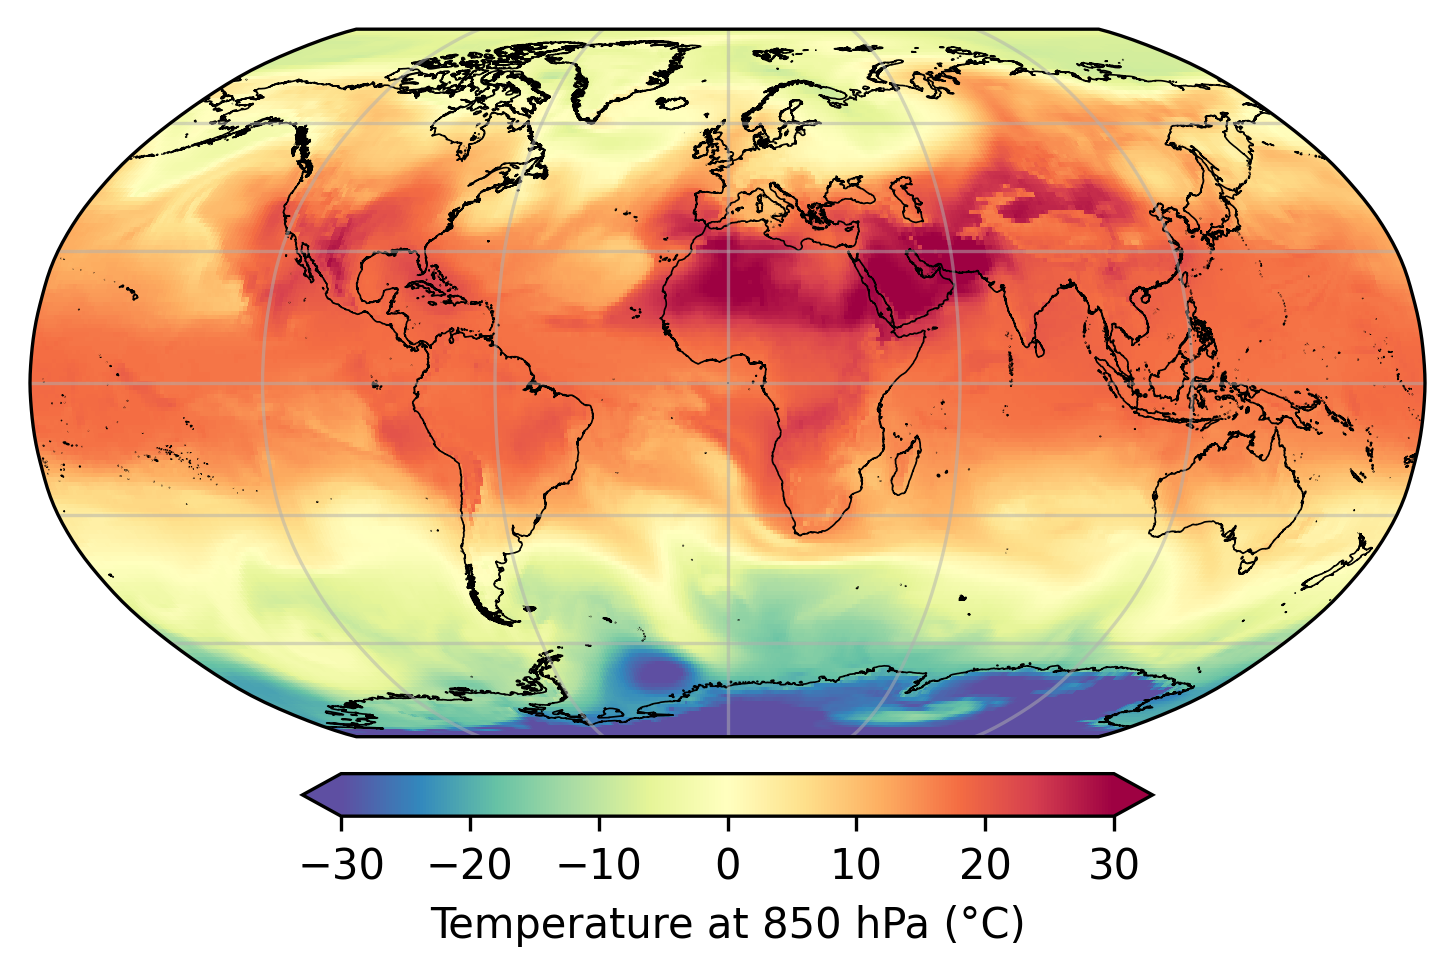
\includegraphics[width=\linewidth]{Chapter2/Figs/eerie_temperature.png}
        \caption{EERIE-AMIP (first member)}
        \label{fig:eerie-esample}
    \end{subfigure}

    \par\medskip

    % Seconda riga: due figure
    \begin{subfigure}{0.49\textwidth}
        \centering
        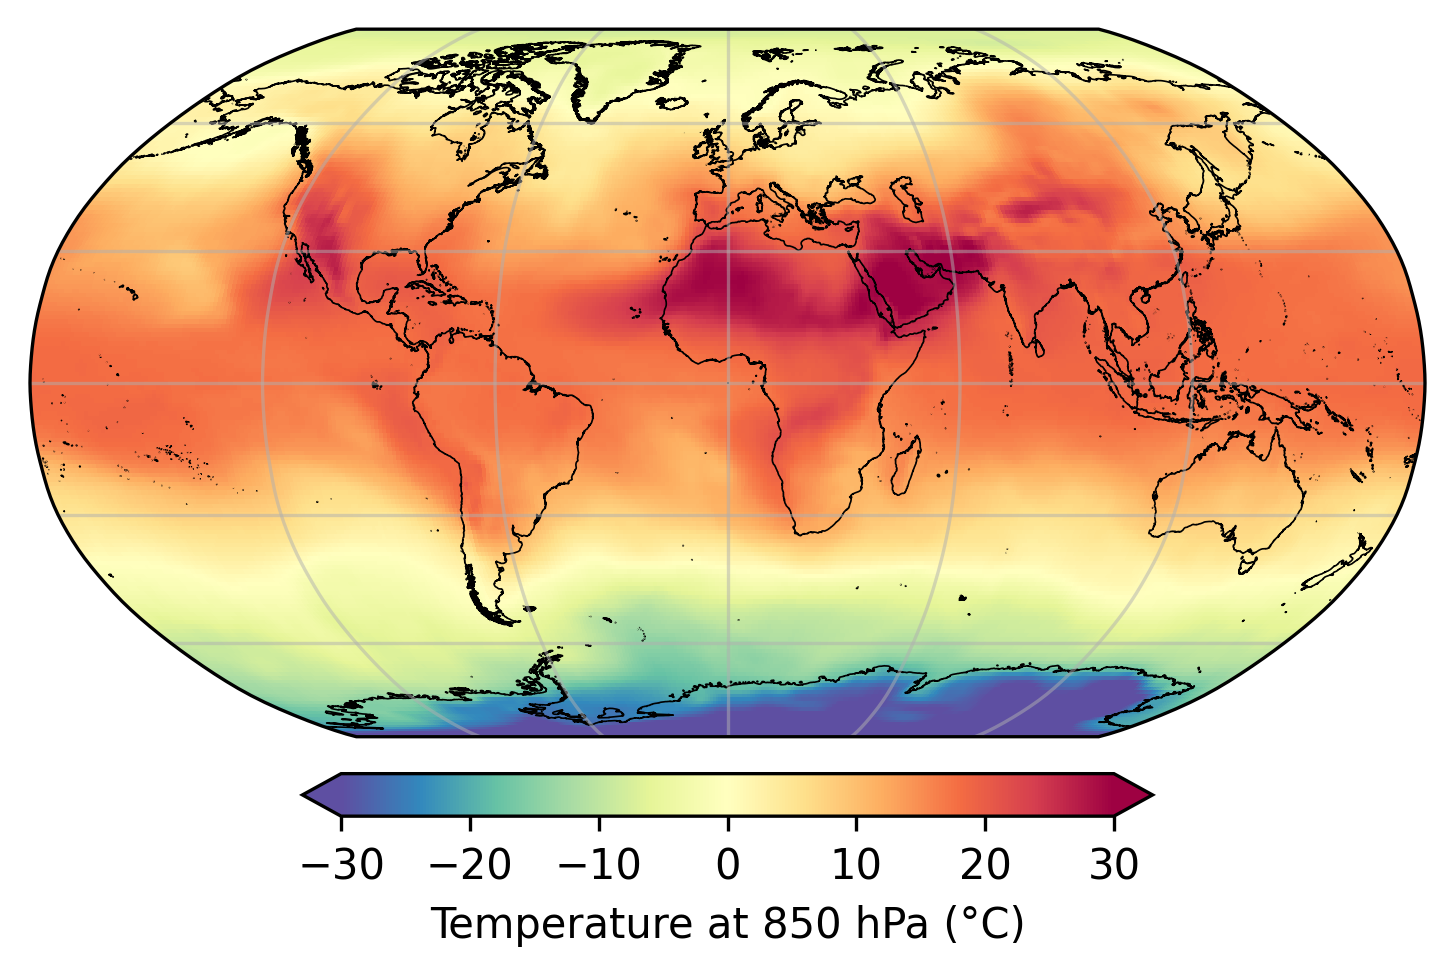
\includegraphics[width=\linewidth]{Chapter2/Figs/ngcm_temperature.png}
        \caption{NeuralGCM ensemble average}
        \label{fig:ngcm-example}
    \end{subfigure}
    \hfill
    \begin{subfigure}{0.49\textwidth}
        \centering
        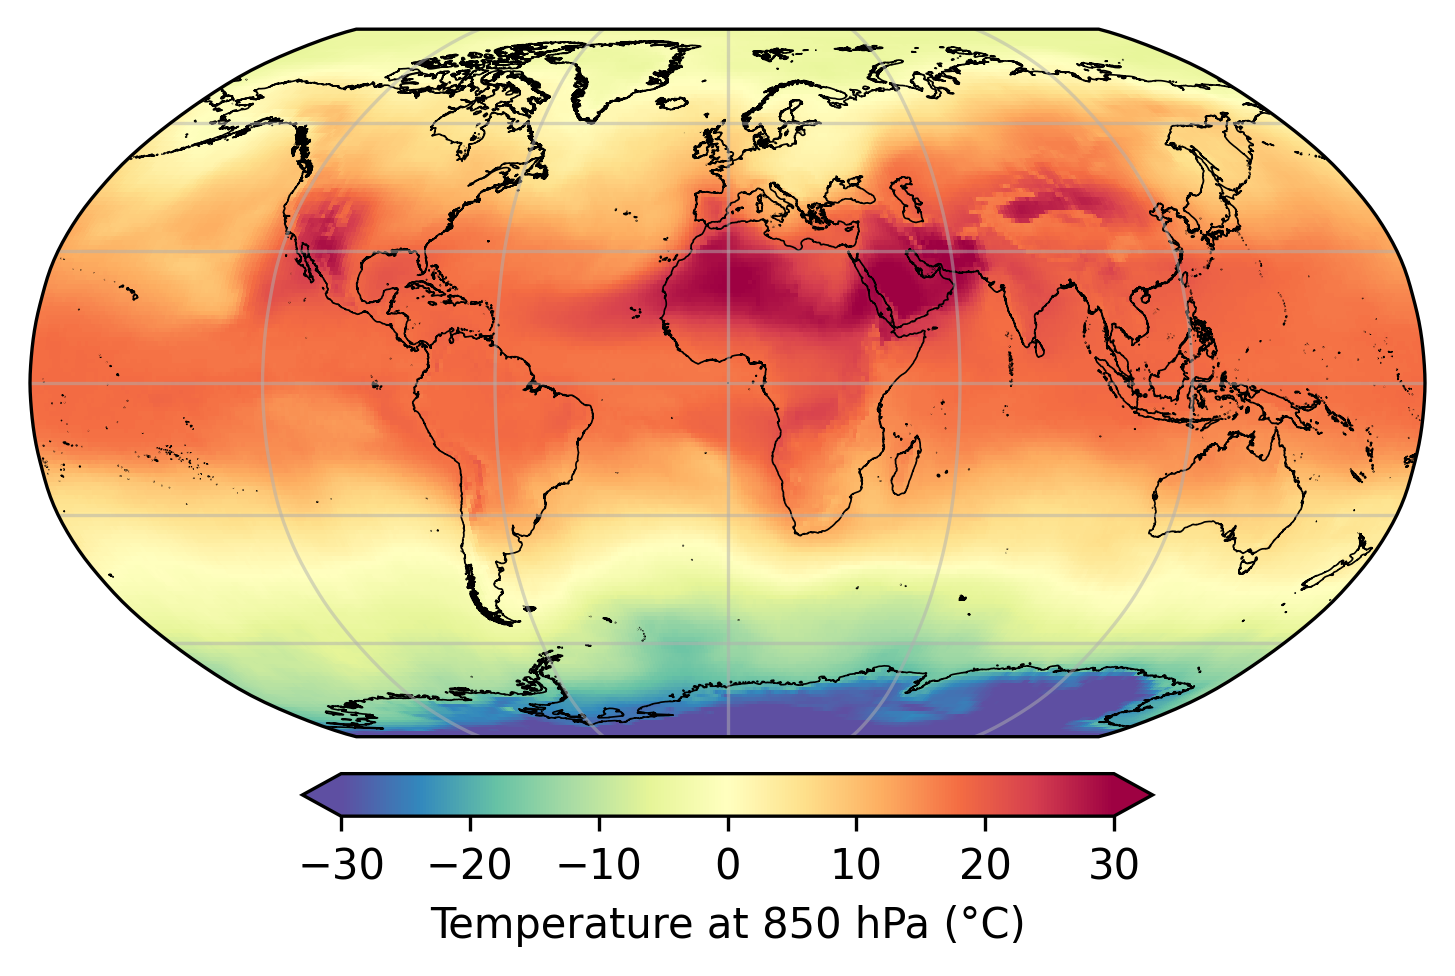
\includegraphics[width=\linewidth]{Chapter2/Figs/aifs_temperature.png}
        \caption{AIFS-CRPS ensemble average}
        \label{fig:aifs-example}
    \end{subfigure}

    \par\medskip

    % Terza riga: due figure
    \begin{subfigure}{0.49\textwidth}
        \centering
        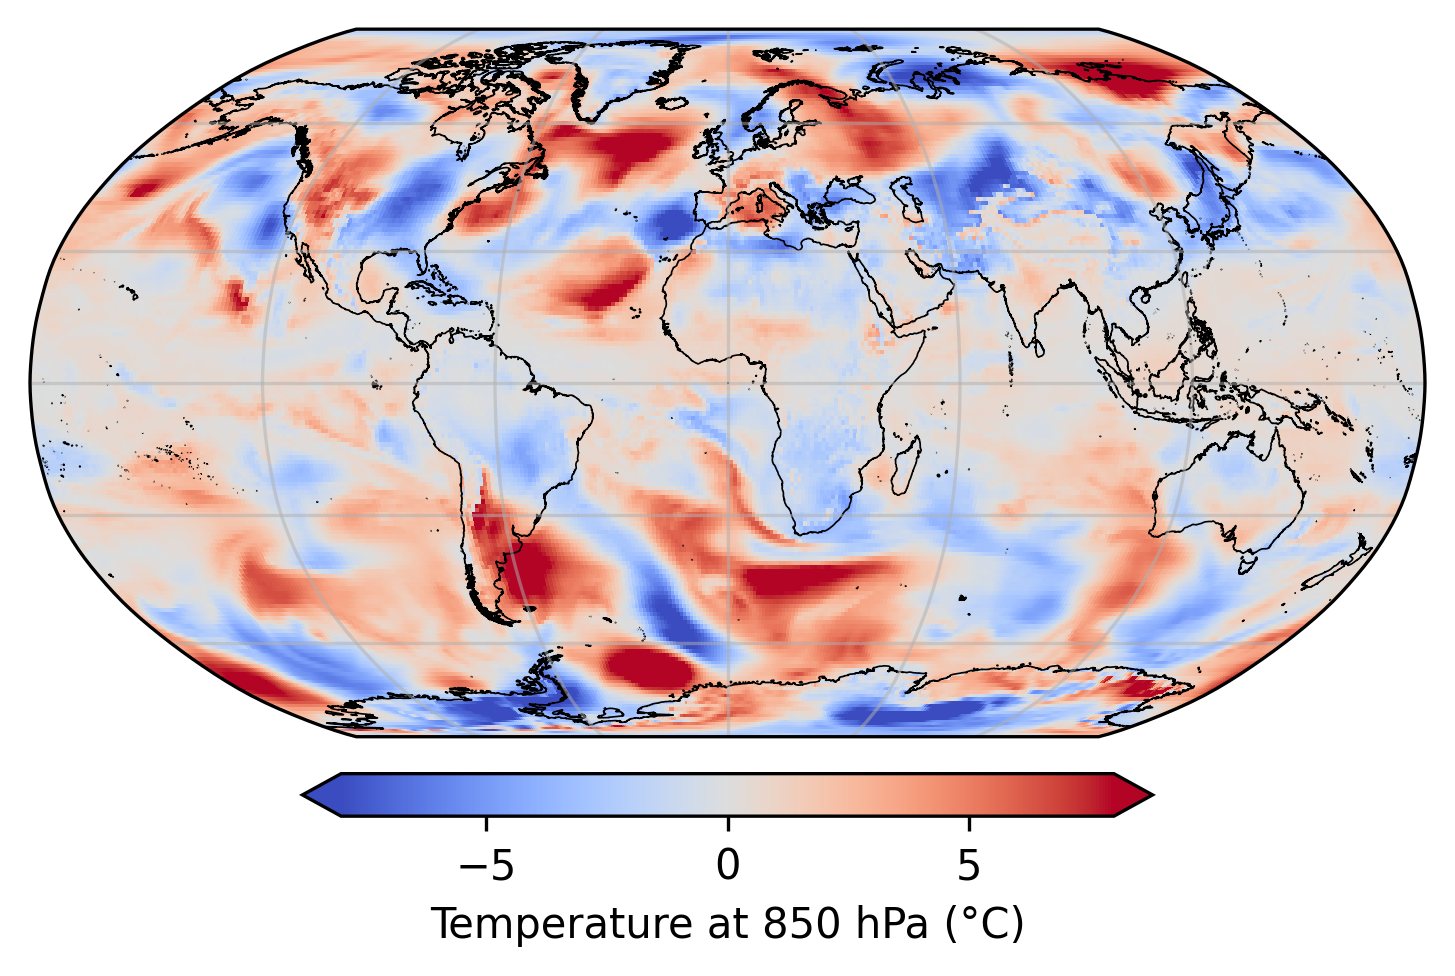
\includegraphics[width=\linewidth]{Chapter2/Figs/ngcm_bias.png}
        \caption{NeuralGCM bias}
        \label{fig:ngcm-bias-example}
    \end{subfigure}
    \hfill
    \begin{subfigure}{0.49\textwidth}
        \centering
        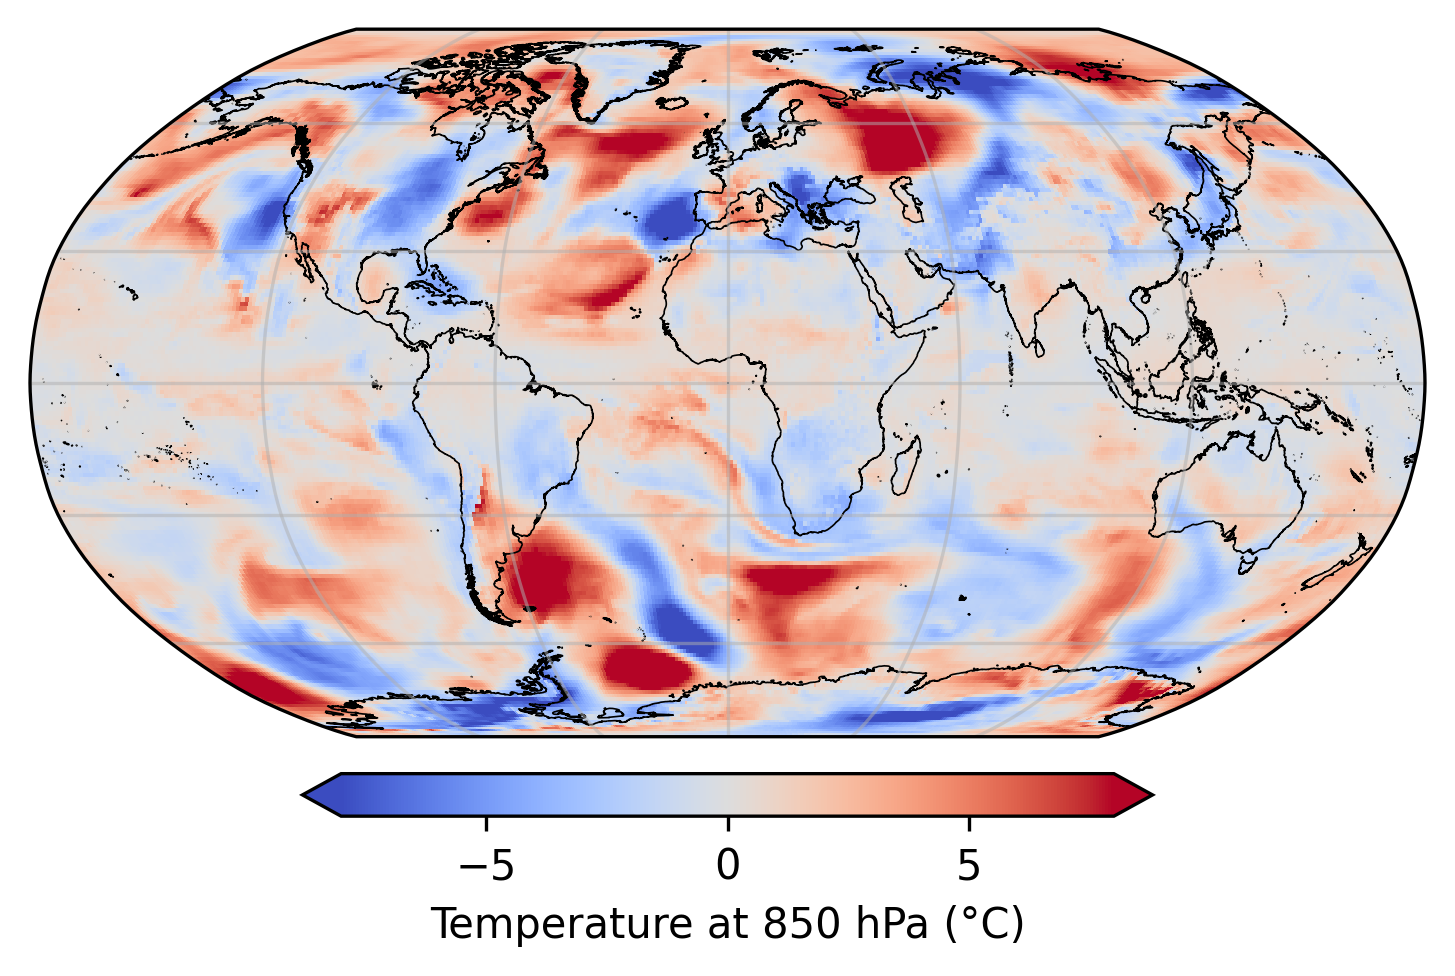
\includegraphics[width=\linewidth]{Chapter2/Figs/aifs_bias.png}
        \caption{AIFS-CRPS bias}
        \label{fig:aifs-bias-example}
    \end{subfigure}

    \caption{Temperature at 850~hPa at a lead time of 10 days for AI forecasts initialized from the EERIE-AMIP first member at June 10th 1987. (a) The verifying EERIE-AMIP member~1 field at the same valid time. (b,c) Ensemble-mean forecasts from NeuralGCM and AIFS-CRPS, respectively, each based on 10 ensemble members. (d,e) Corresponding ensemble-mean temperature differences relative to EERIE-AMIP member~1.}
    \label{fig:example-inference-maps}
    
\end{figure}


\begin{figure}[H]
    \begin{subfigure}{1\textwidth}
        \centering
        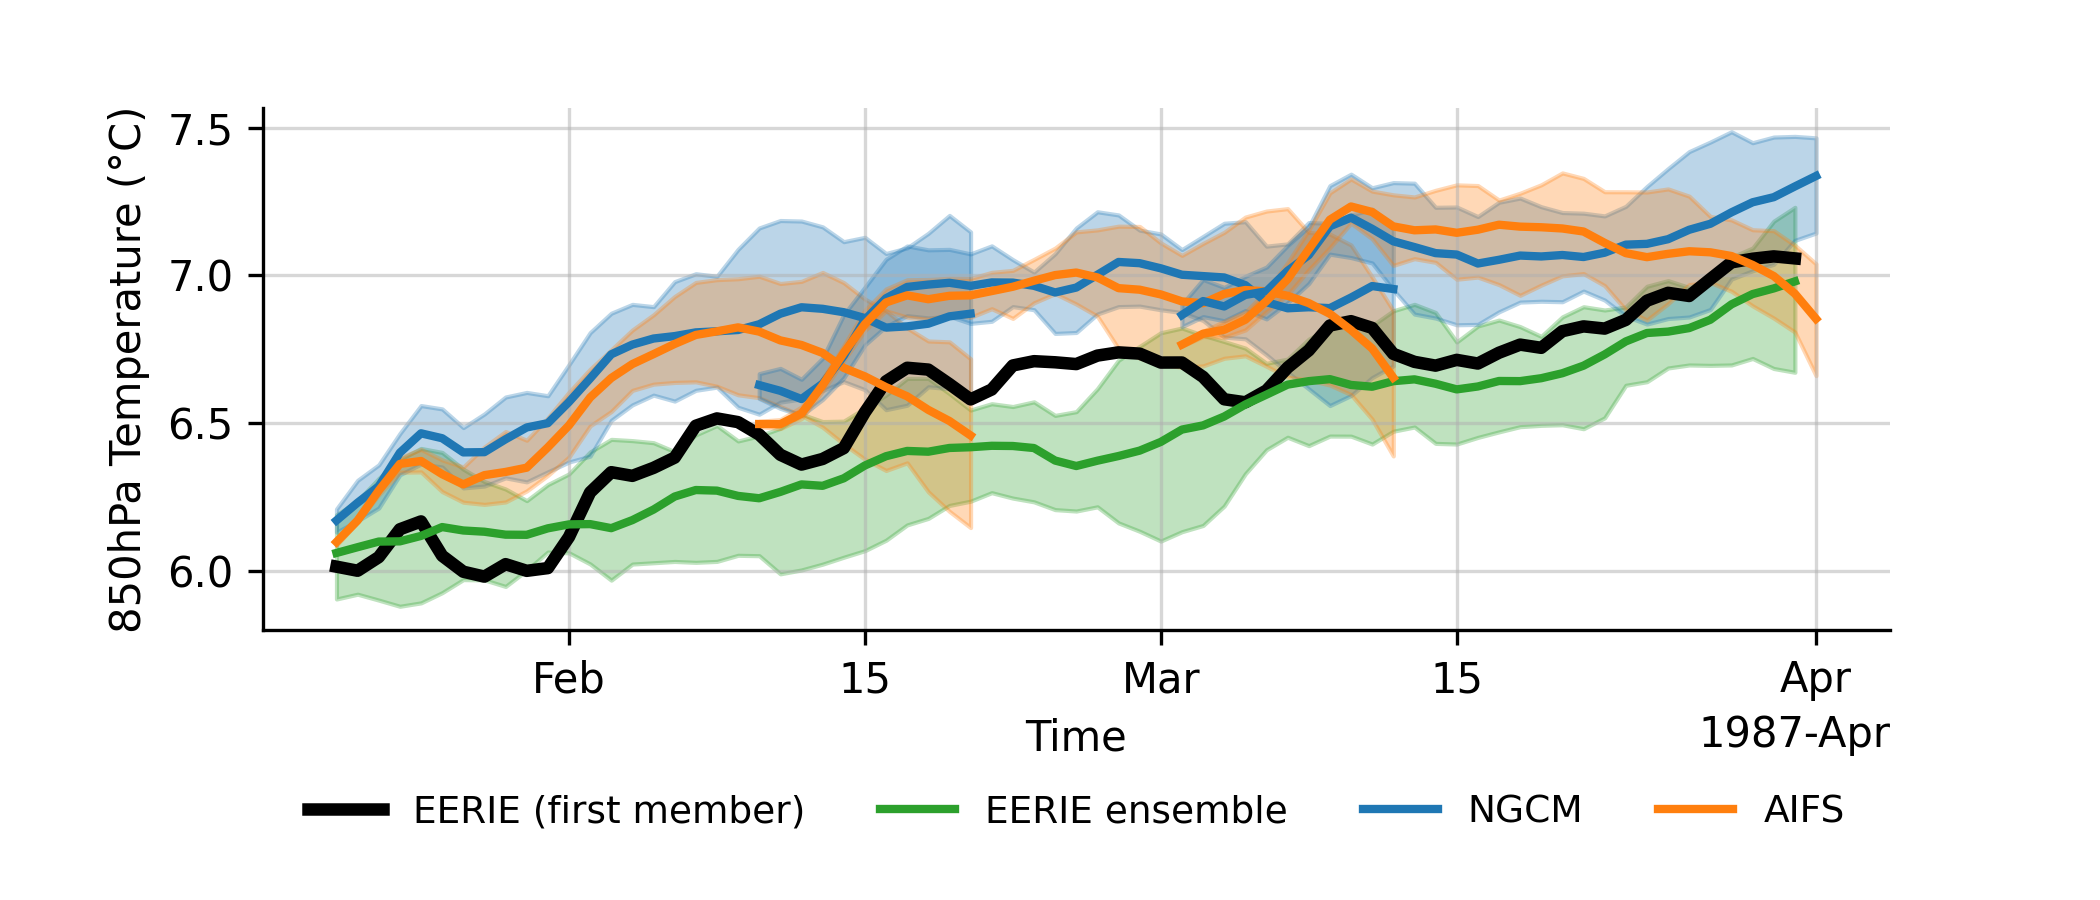
\includegraphics[width=0.8\linewidth]{Chapter2//Figs/cool_lines_plot_winter.png}
        \caption{Winter 1987.}
        \label{fig:global-temperature-winter}
    \end{subfigure}

    \par\medskip

    \begin{subfigure}{1\textwidth}
        \centering
        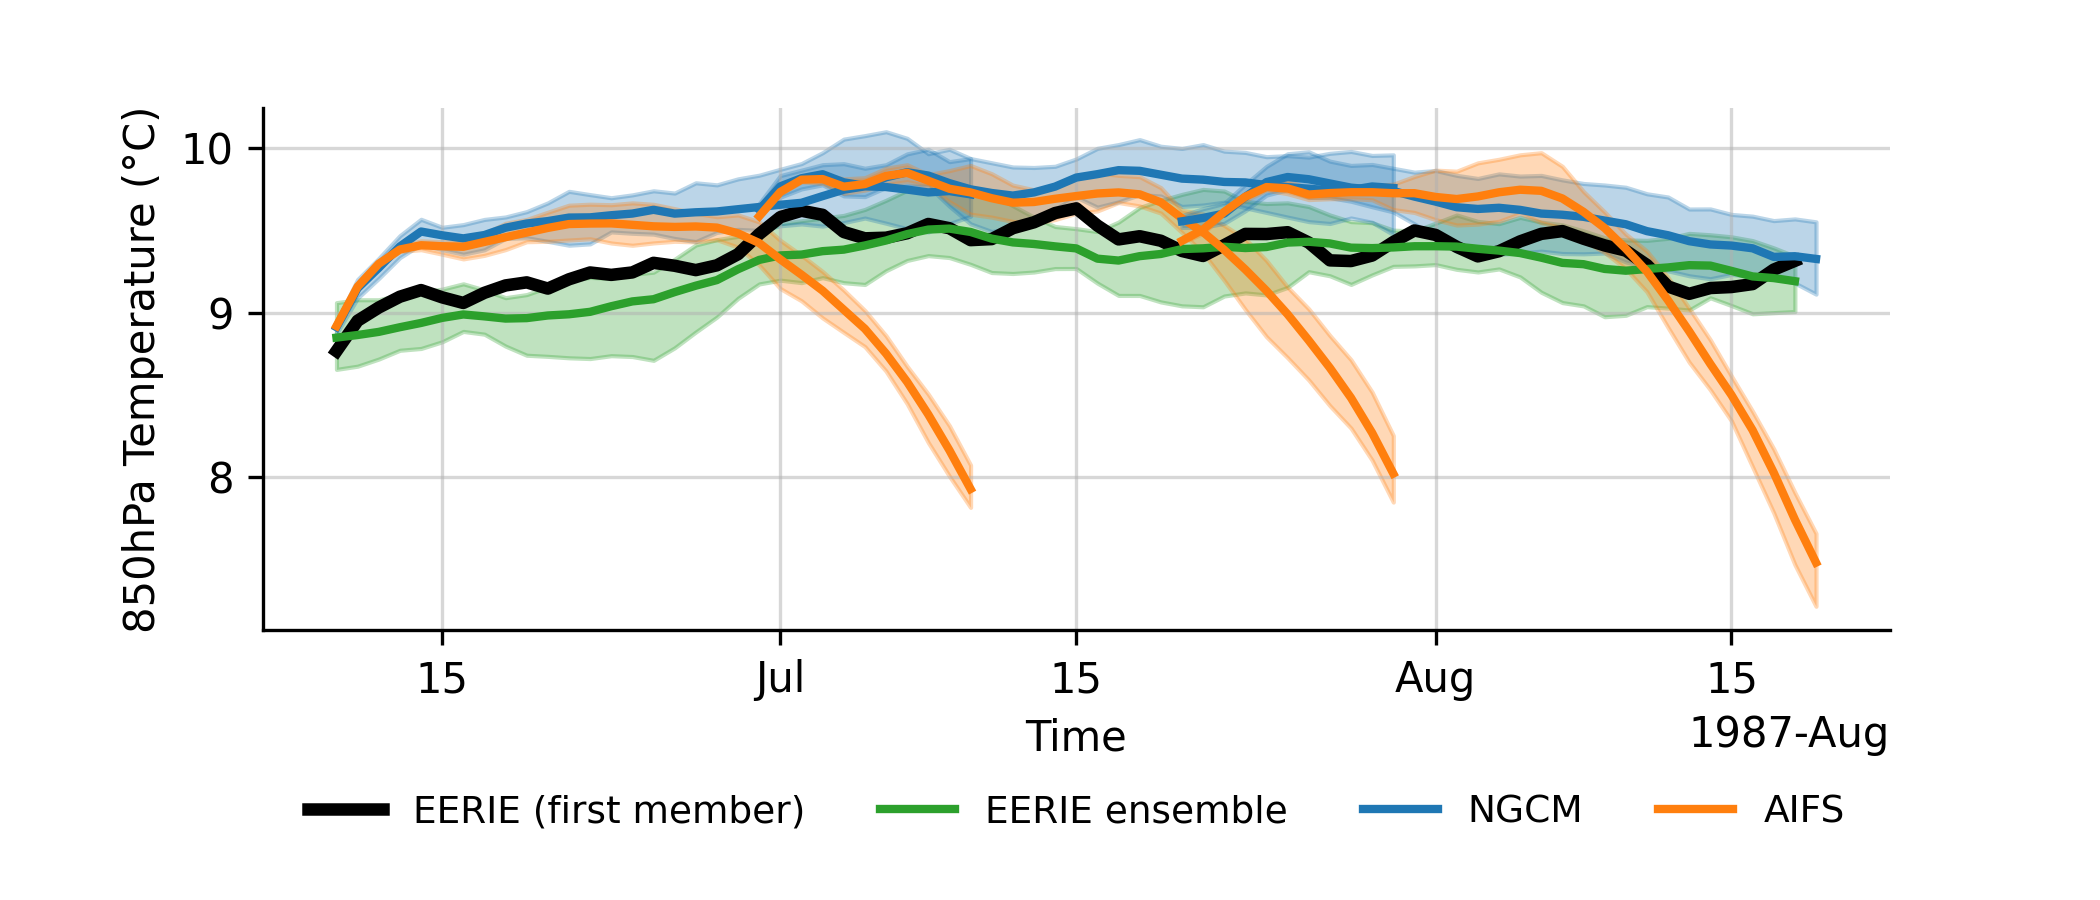
\includegraphics[width=0.8\linewidth]{Chapter2//Figs/cool_lines_plot_summer.png}
        \caption{Summer 1987.}
        \label{fig:global-temperature-summer}
    \end{subfigure}

    \caption{Global mean temperature at 850~hPa. The black line shows EERIE-AMIP member 1, which provides the initial conditions for the AI forecasts, while the green line represents the mean of the remaining nine EERIE-AMIP members. Blue and orange lines show the ensemble means of NeuralGCM and AIFS-CRPS. The forecasts have been initialized on 21 January, 10 February, and 2 March 1987 (panel a) and on June 10, June 30 and July 20 1987 (panel b). Shaded bands indicate the 5th--95th percentile range across the corresponding ensemble members, calculated from their individual global mean temperatures.}
    \label{fig:global-temperature}
    
\end{figure}


\begin{figure}[H]
    \centering
    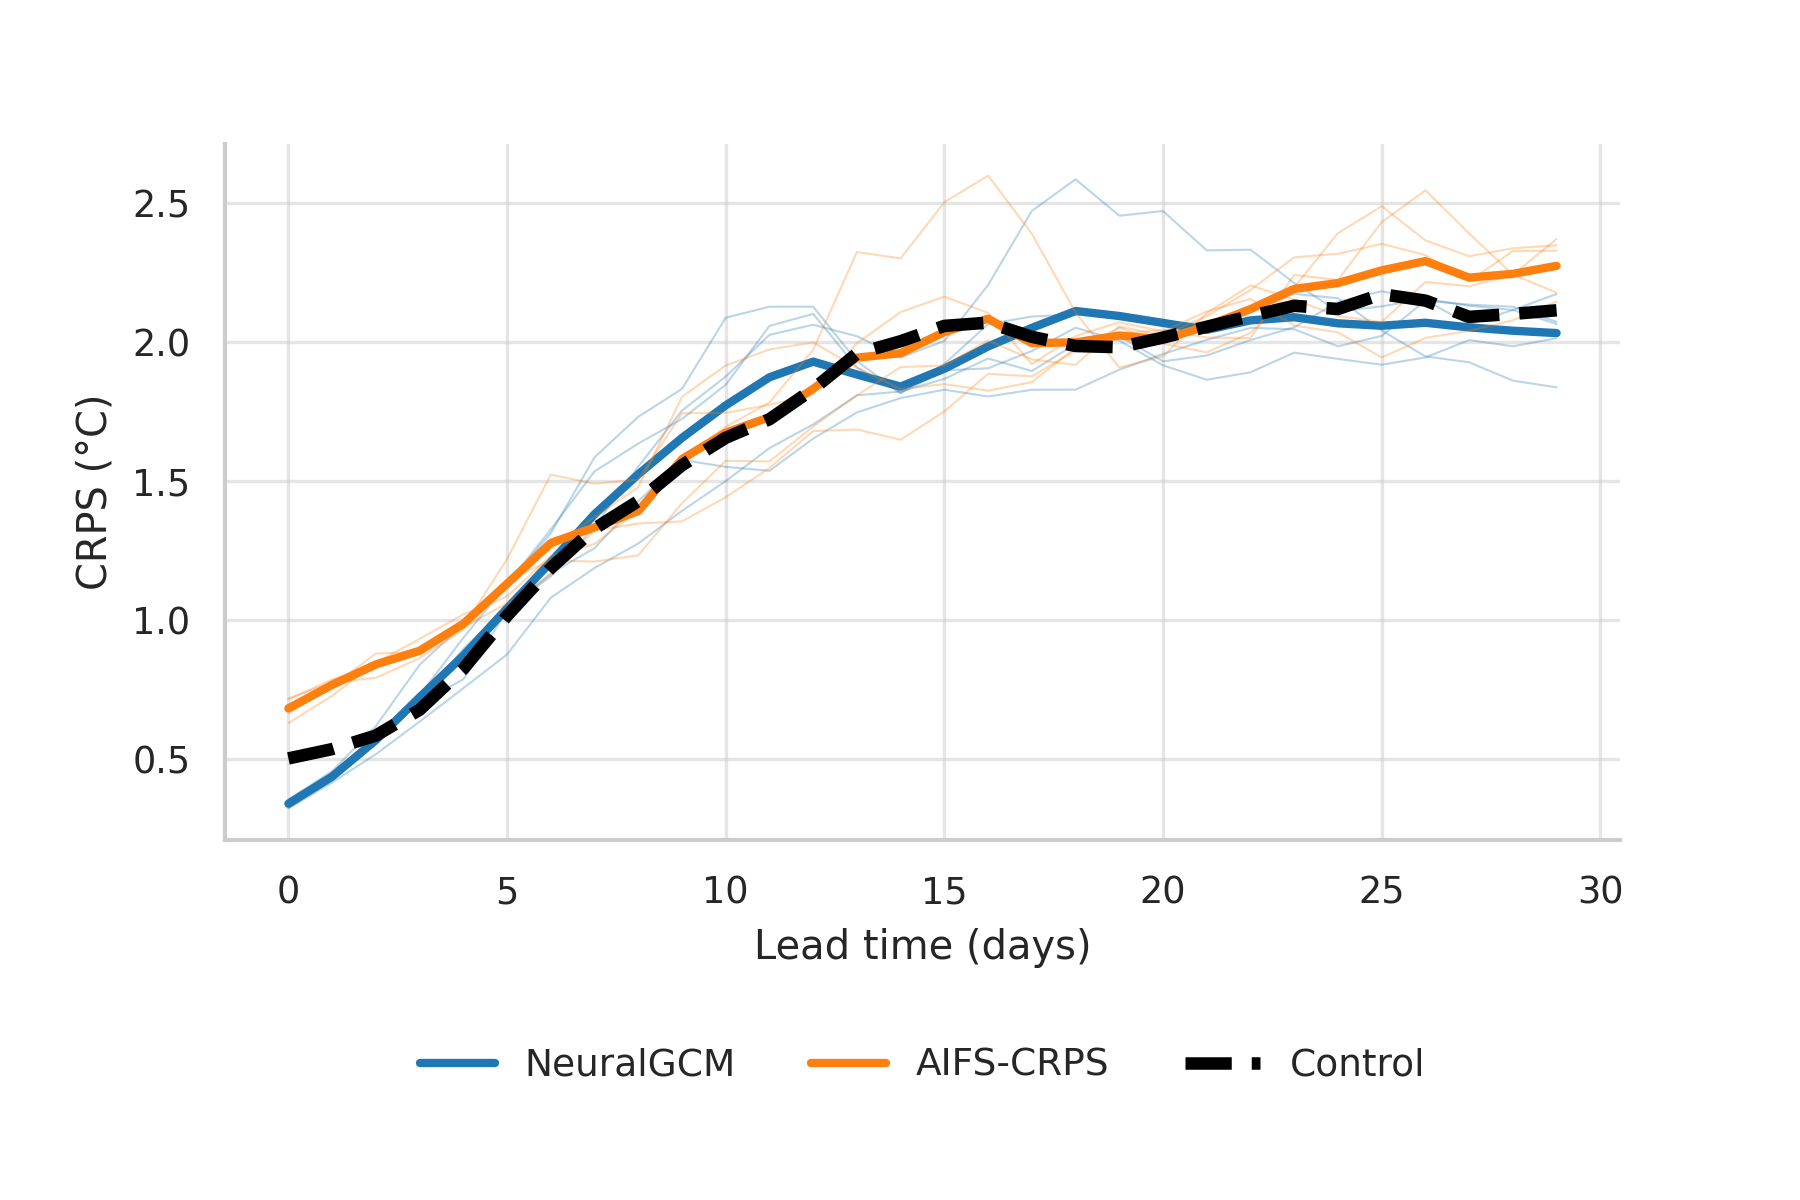
\includegraphics[width=0.75\linewidth]{Chapter2//Figs/crps_global.png}
    \caption{Spatially averaged CRPS of 850 hPa temperature as a function of forecast lead time. NeuralGCM and AIFS ensemble forecasts are verified against the first member of EERIE-AMIP for two randomly selected initialization dates in 1985--1990. Thin lines show the CRPS for each initialization date; thick lines show the mean across the selected EERIE initializations. The dashed black control line shows the mean CRPS of NeuralGCM-ERA against ERA5 across eight initialization dates randomly selected in 1985.}
    \label{fig:crps}
\end{figure}

\begin{figure}[p]
    \centering

    % Prima riga: una figura centrata
    \begin{subfigure}{1\textwidth}
        \centering
        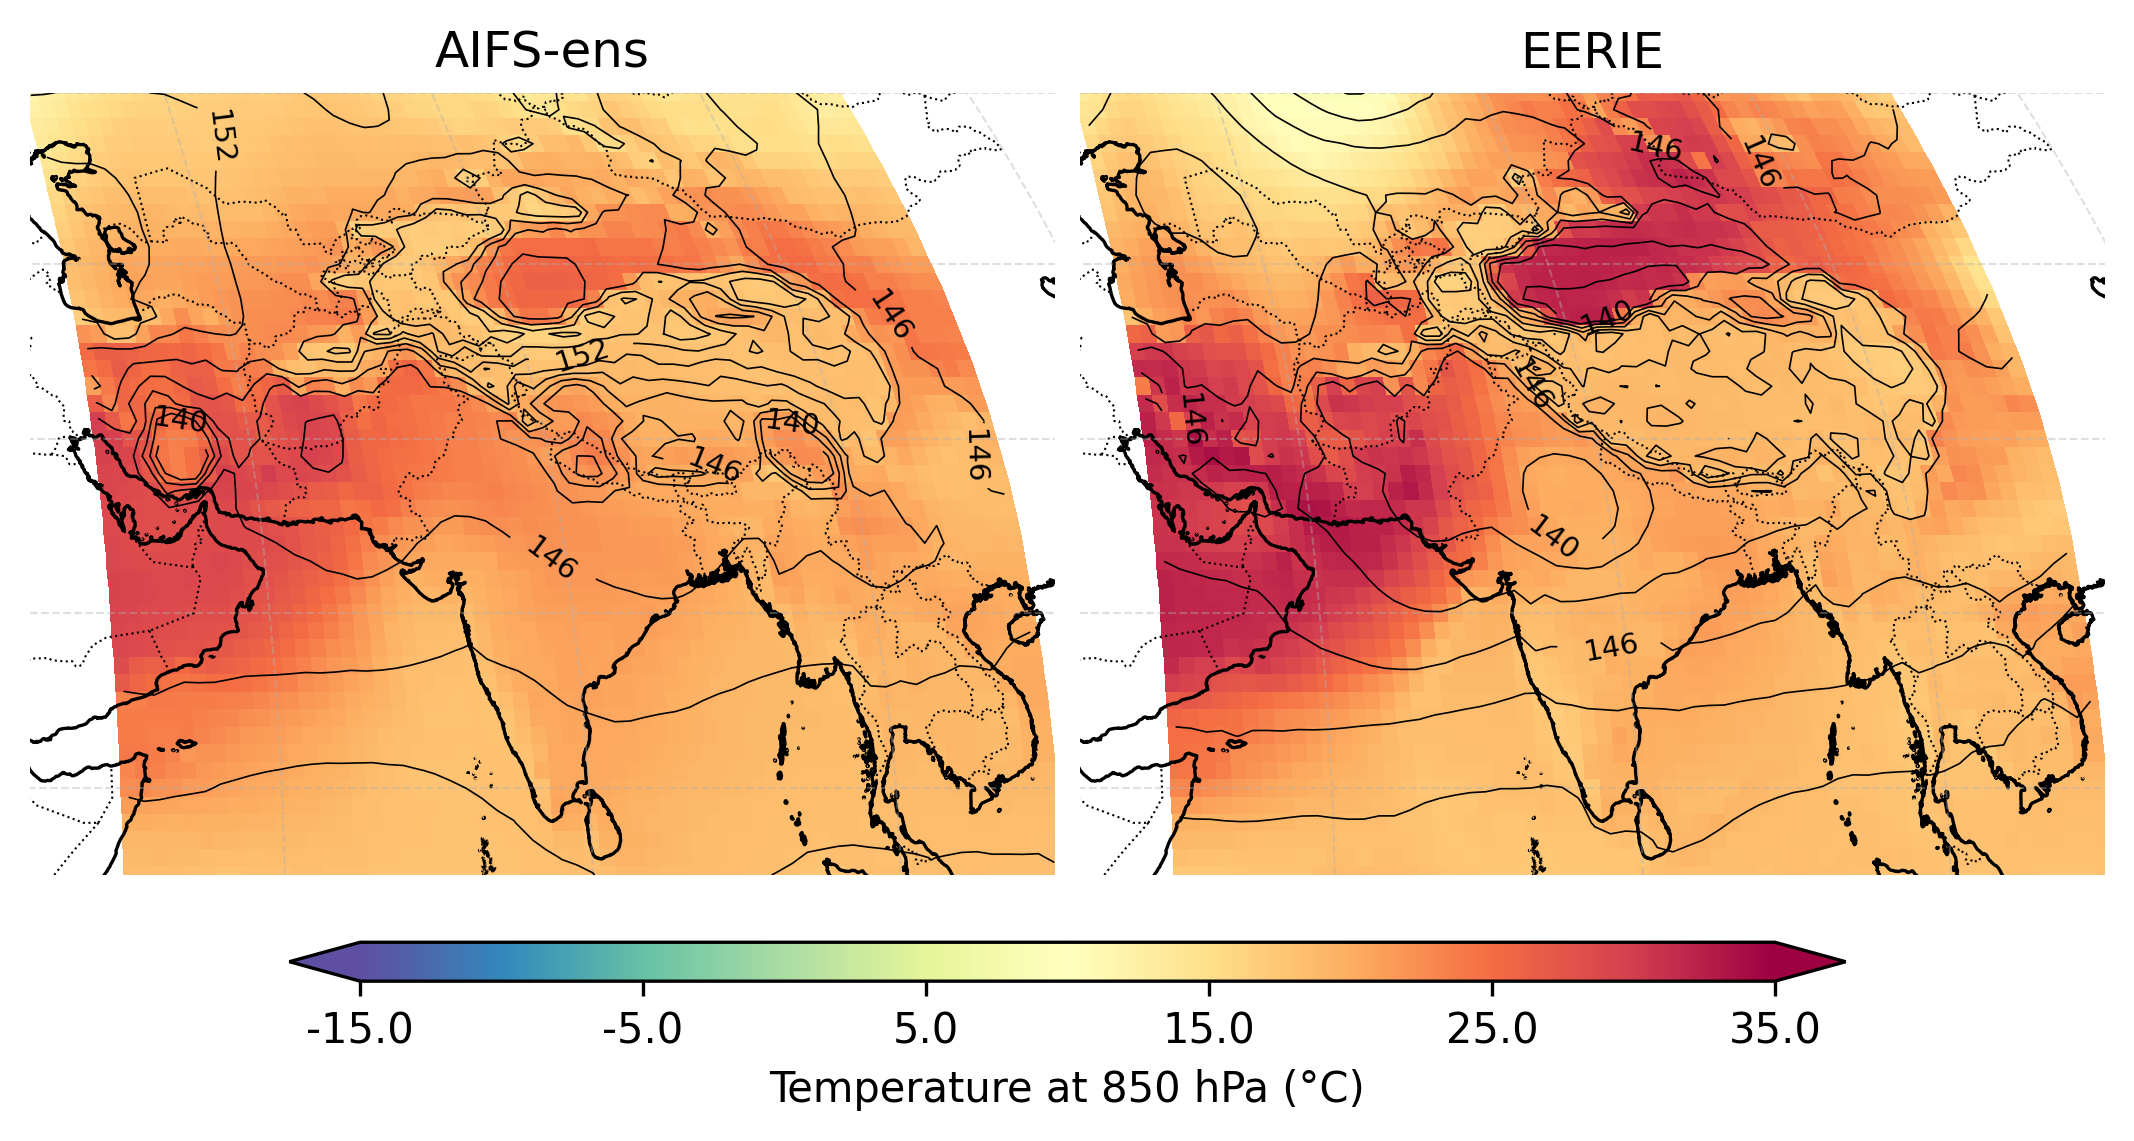
\includegraphics[width=0.6\linewidth]{Chapter2/Figs/comparison_ens_aifs_15_India.png}
        \caption{Lead time: 5 days}
        \label{fig:5-days-india}
    \end{subfigure}

    \par\medskip

    \begin{subfigure}{1\textwidth}
        \centering
        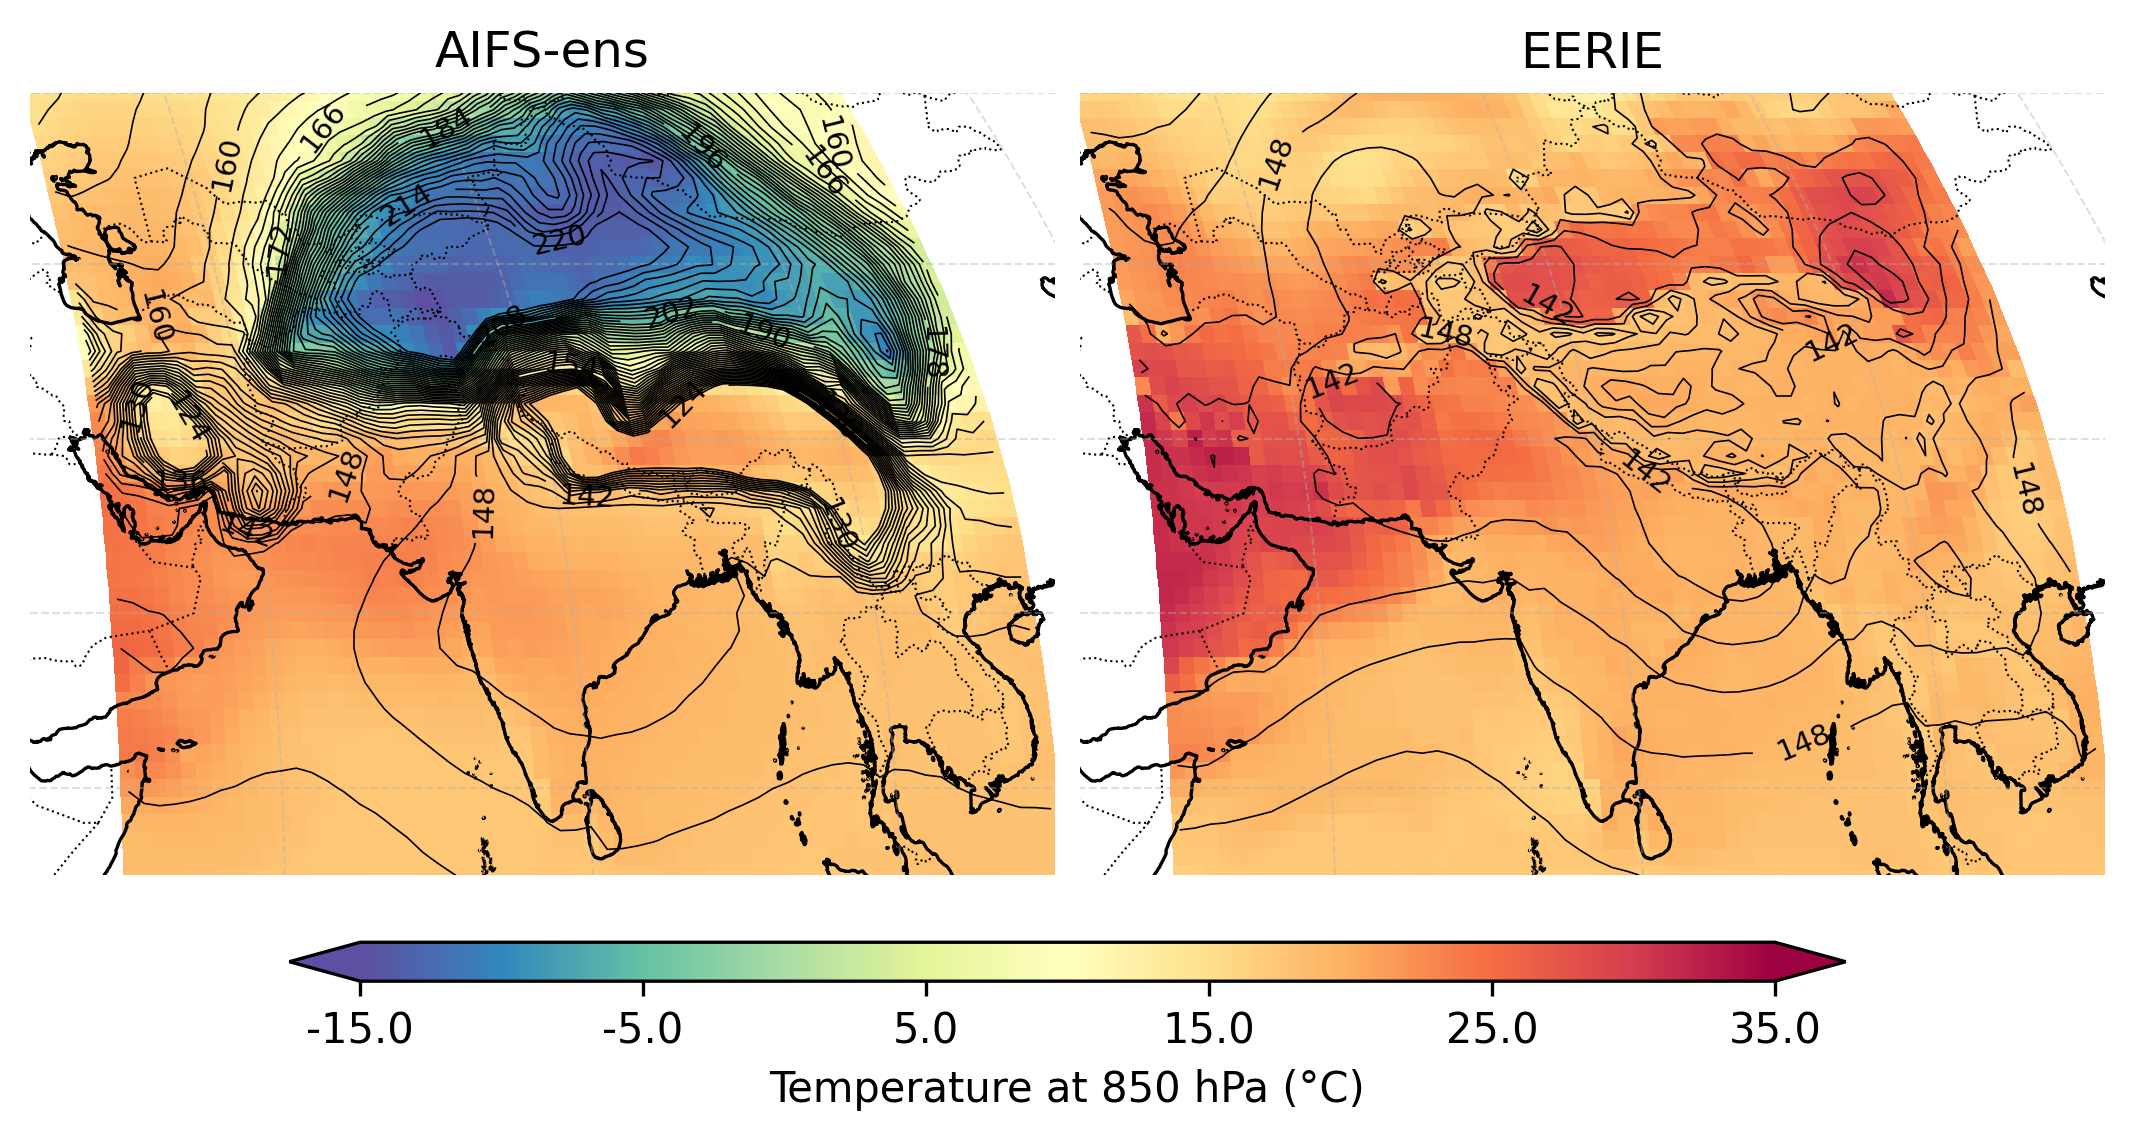
\includegraphics[width=0.6\linewidth]{Chapter2/Figs/comparison_ens_aifs_25_India.png}
        \caption{Lead time: 25 days}
        \label{fig:25-days-india}
    \end{subfigure}


    \par\medskip

    \begin{subfigure}{1\textwidth}
        \centering
        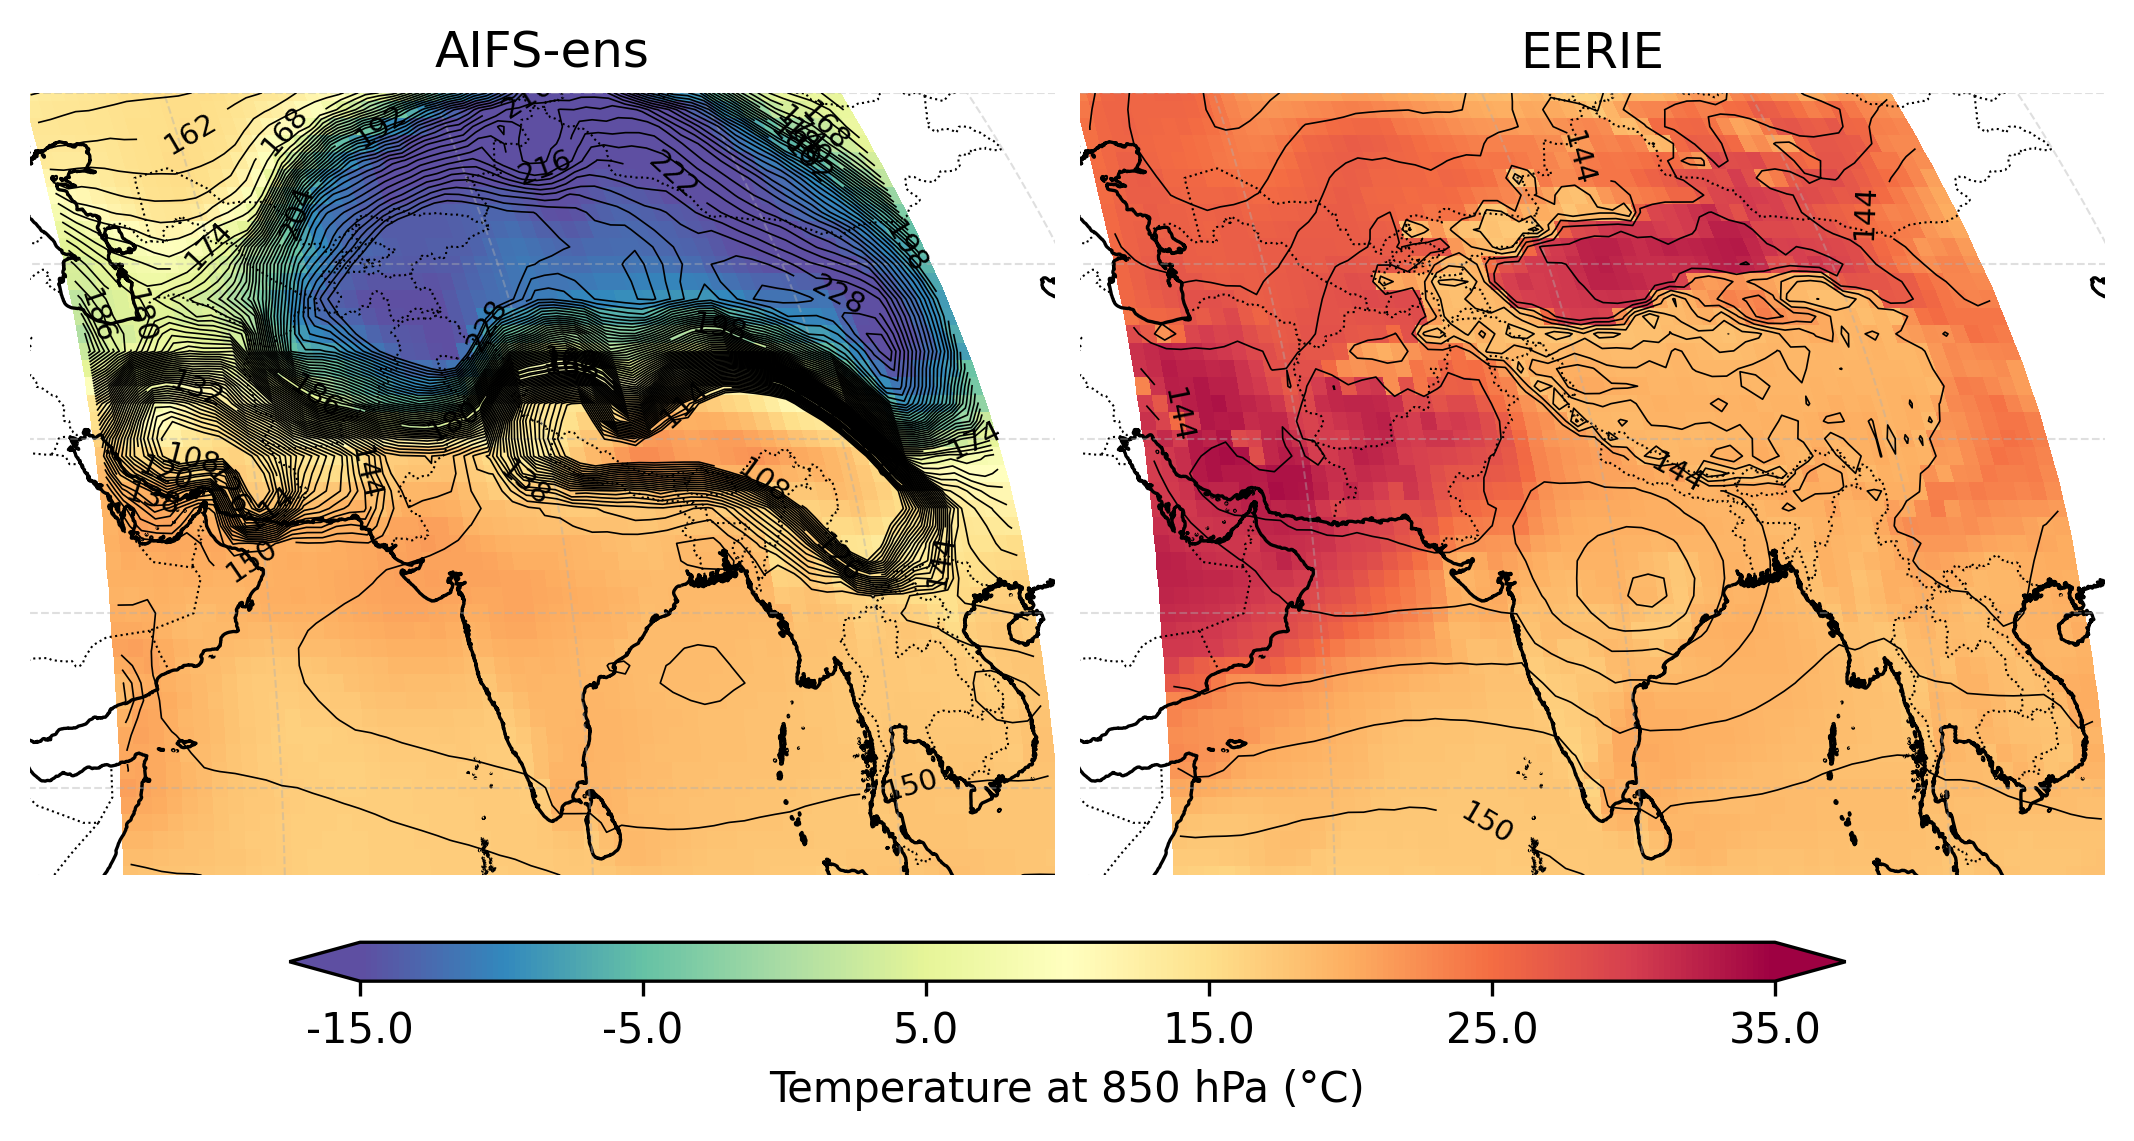
\includegraphics[width=0.6\linewidth]{Chapter2/Figs/comparison_ens_aifs_29_India.png}
        \caption{Lead time: 29 days}
        \label{fig:29-days-india}
    \end{subfigure}

    \caption{Development of an anomalous pattern over the Himalayan region in an AIFS-CRPS forecast initialized on 10 June 1987. Panels show the 10-member ensemble mean at lead times of (a) 15, (b) 25, and (c) 29 days. Shading represents temperature at 850~hPa, while contours indicate geopotential height at the same pressure level, expressed in decametres (dam).}
    \label{fig:example-aifs-degenerative}
\end{figure}

\clearpage

\subsection{AI Model Climatology}

The climatological evaluation examines whether forecasts initialized from EERIE-AMIP preserve the mean climatic conditions of the source simulation as lead time increases. Comparisons with EERIE-AMIP and ERA5 provide complementary information: the former assesses consistency with the initialization dataset, while the latter indicates how closely the generated fields resemble the reanalysis used to train the AI models. 

Figure~\ref{fig:climatology-lines} shows the annual cycle of global mean temperature at 850~hPa, using forecast lead times between 10 and 20 days for the AI models. Both NeuralGCM and AIFS-CRPS reproduce the timing and amplitude of the seasonal cycle, with a minimum during boreal winter and a maximum in July. Despite being initialized from EERIE-AMIP, their global mean temperatures remain closer to ERA5 throughout most of the year. Differences relative to ERA5 are generally limited to a few tenths of a degree, whereas both models are approximately $0.2$--$0.5\,^{\circ}\mathrm{C}$ warmer than EERIE-AMIP. The agreement between the two AI models is therefore accompanied by a common departure from the mean state of their initialization dataset.

\begin{figure}[H]
    \centering
    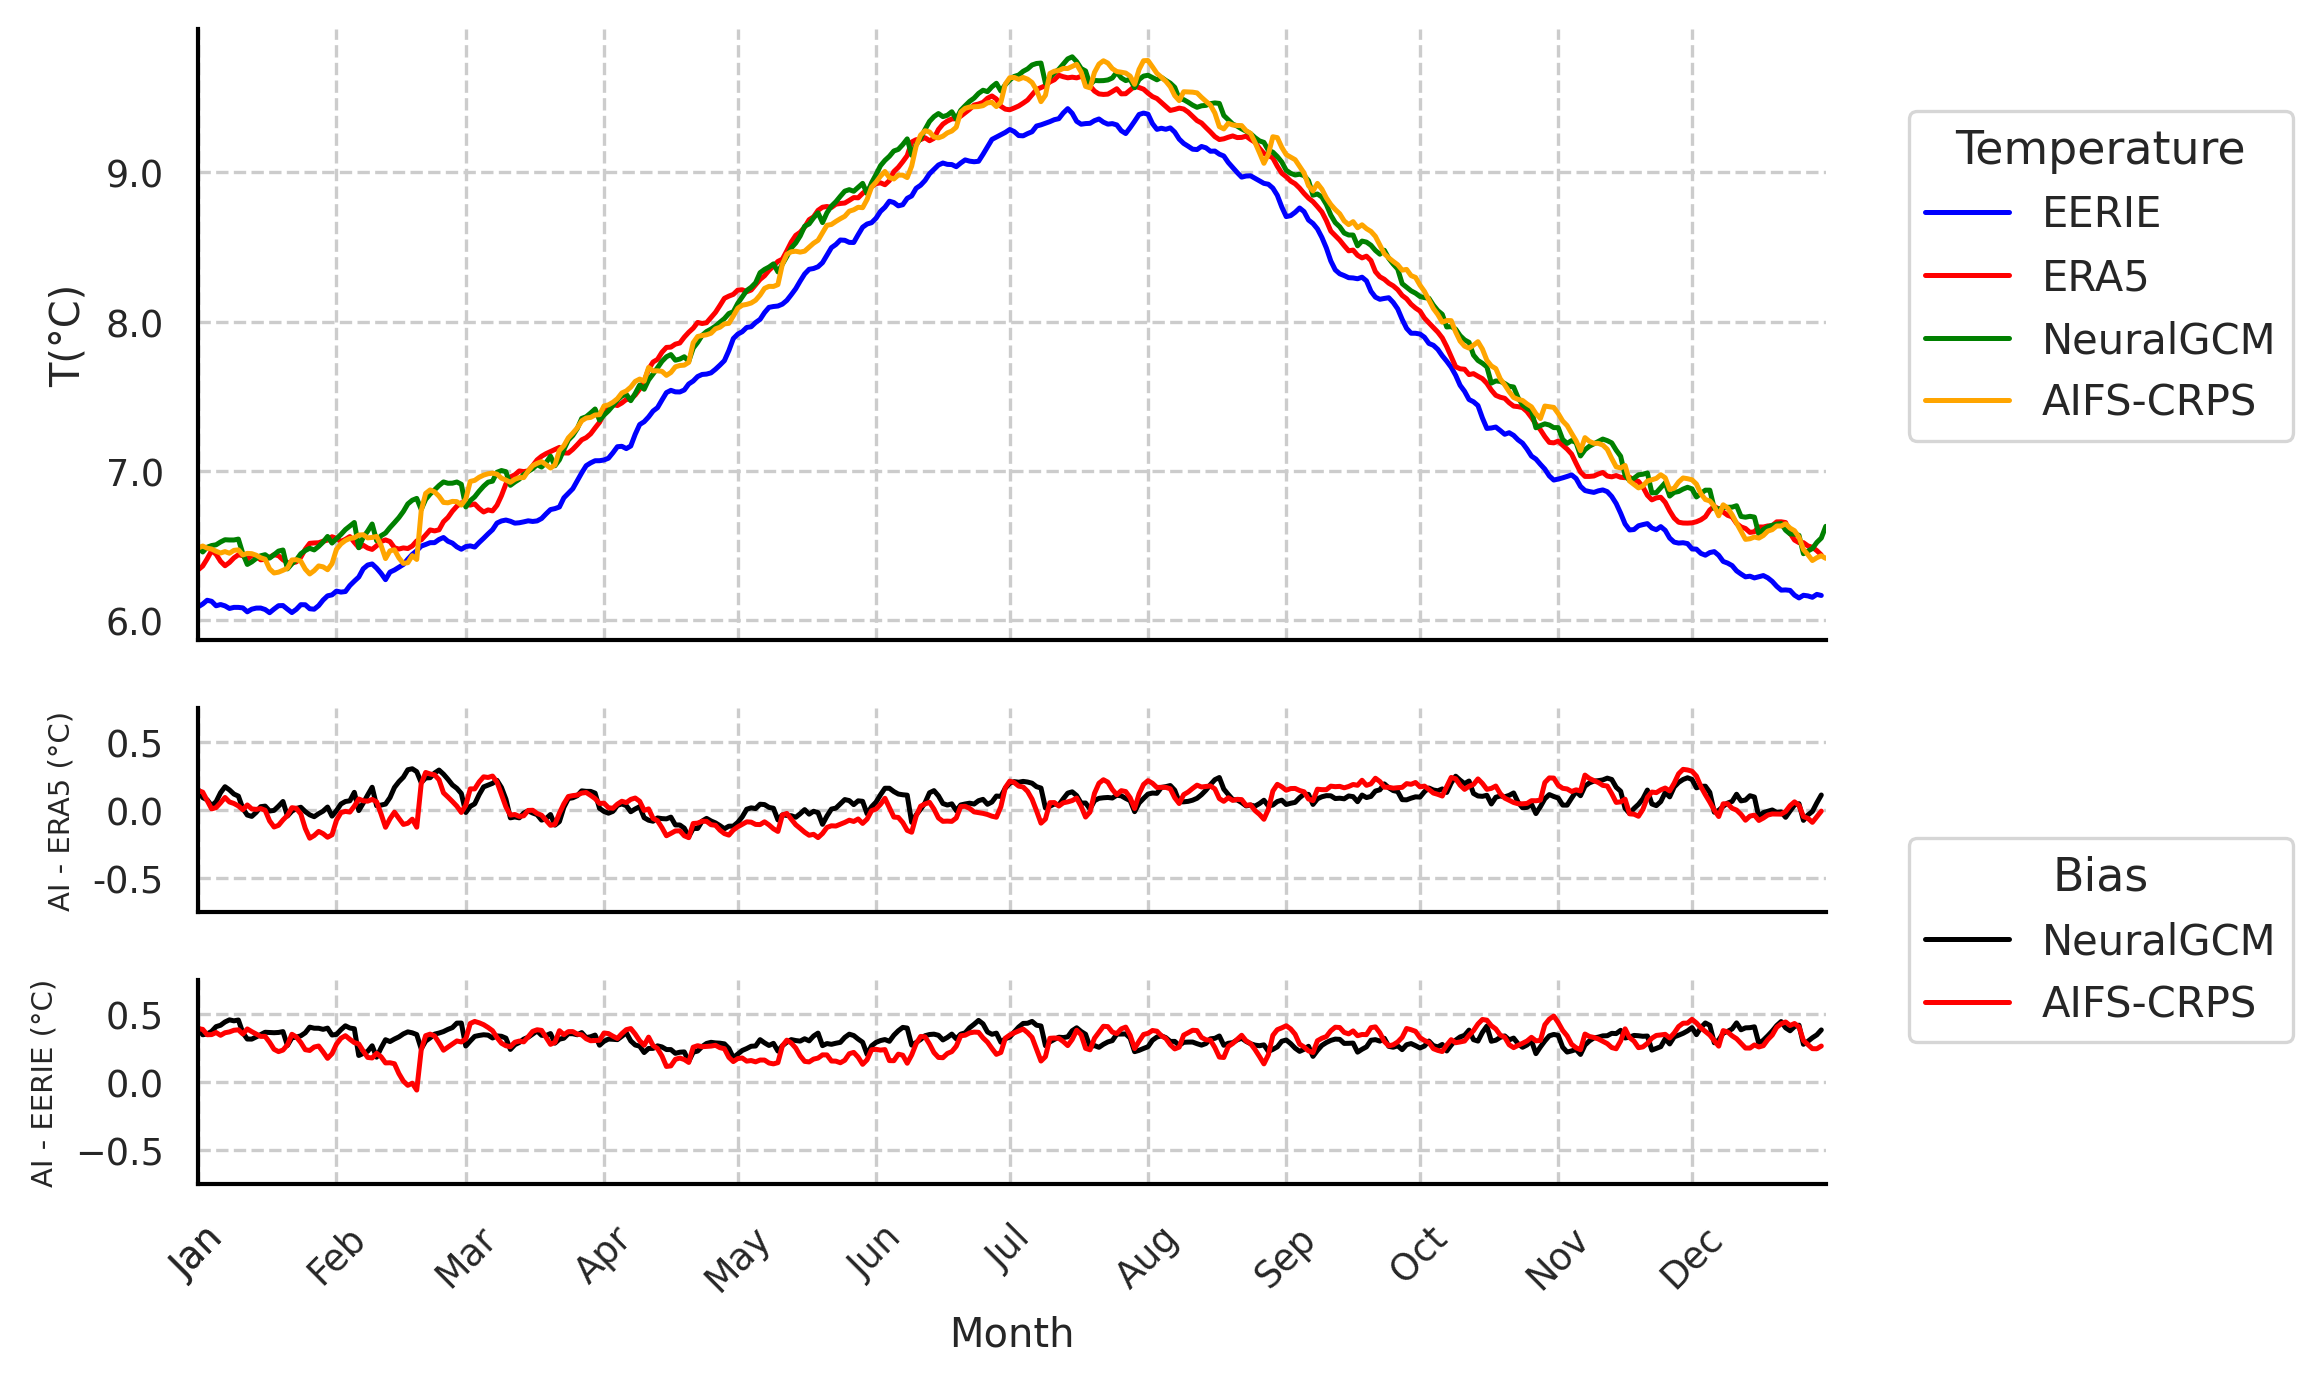
\includegraphics[width=0.8\linewidth]{Chapter2//Figs/climatologie_lines.png}
    \caption{Climatological annual cycle of air temperature at 850~hPa over the period 1981--1990. The upper panel compares the daily climatologies produced by EERIE, ERA5, NeuralGCM, and AIFS-CRPS. For the AI weather models, the climatology is computed using forecast lead times between 10 and 20 days. This interval is selected heuristically to represent the window between the decay of the influence of the initial conditions and the point at which the forecasts begin to lose stability. The middle and lower panels show the temperature differences of the two AI-based models relative to ERA5 and EERIE, respectively.}
    \label{fig:climatology-lines}
\end{figure}

The lead-time-dependent biases in Figure~\ref{fig:climatology-bias} show how this departure develops. NeuralGCM exhibits a predominantly positive bias relative to EERIE-AMIP from the first five-day window onwards. The annual mean bias increases during the initial forecast stages and subsequently remains around $+0.3$--$0.4\,^{\circ}\mathrm{C}$. Relative to ERA5, the annual mean bias is substantially smaller and remains slightly positive after the first five days. Monthly differences nevertheless reveal a seasonal structure, with larger warm biases towards the end of the year. NeuralGCM therefore maintains a comparatively stable global mean over the 30-day integration, but this mean differs systematically from that of EERIE-AMIP.

AIFS-CRPS initially follows a similar pattern, with a small annual mean bias relative to ERA5 and a positive bias relative to EERIE-AMIP. After approximately 20 days, however, its behaviour changes. A cold bias develops, particularly between May and September, and intensifies in the final forecast window. By days 25--30, the annual mean bias is approximately $-0.5\,^{\circ}\mathrm{C}$ relative to ERA5 and $-0.3\,^{\circ}\mathrm{C}$ relative to EERIE-AMIP, while several monthly biases extend beyond the lower limit of the colour scale. This confirms that the cooling identified in the individual forecasts is a recurring, seasonally dependent feature of the evaluated configuration.

\begin{figure}[H]
    \centering
    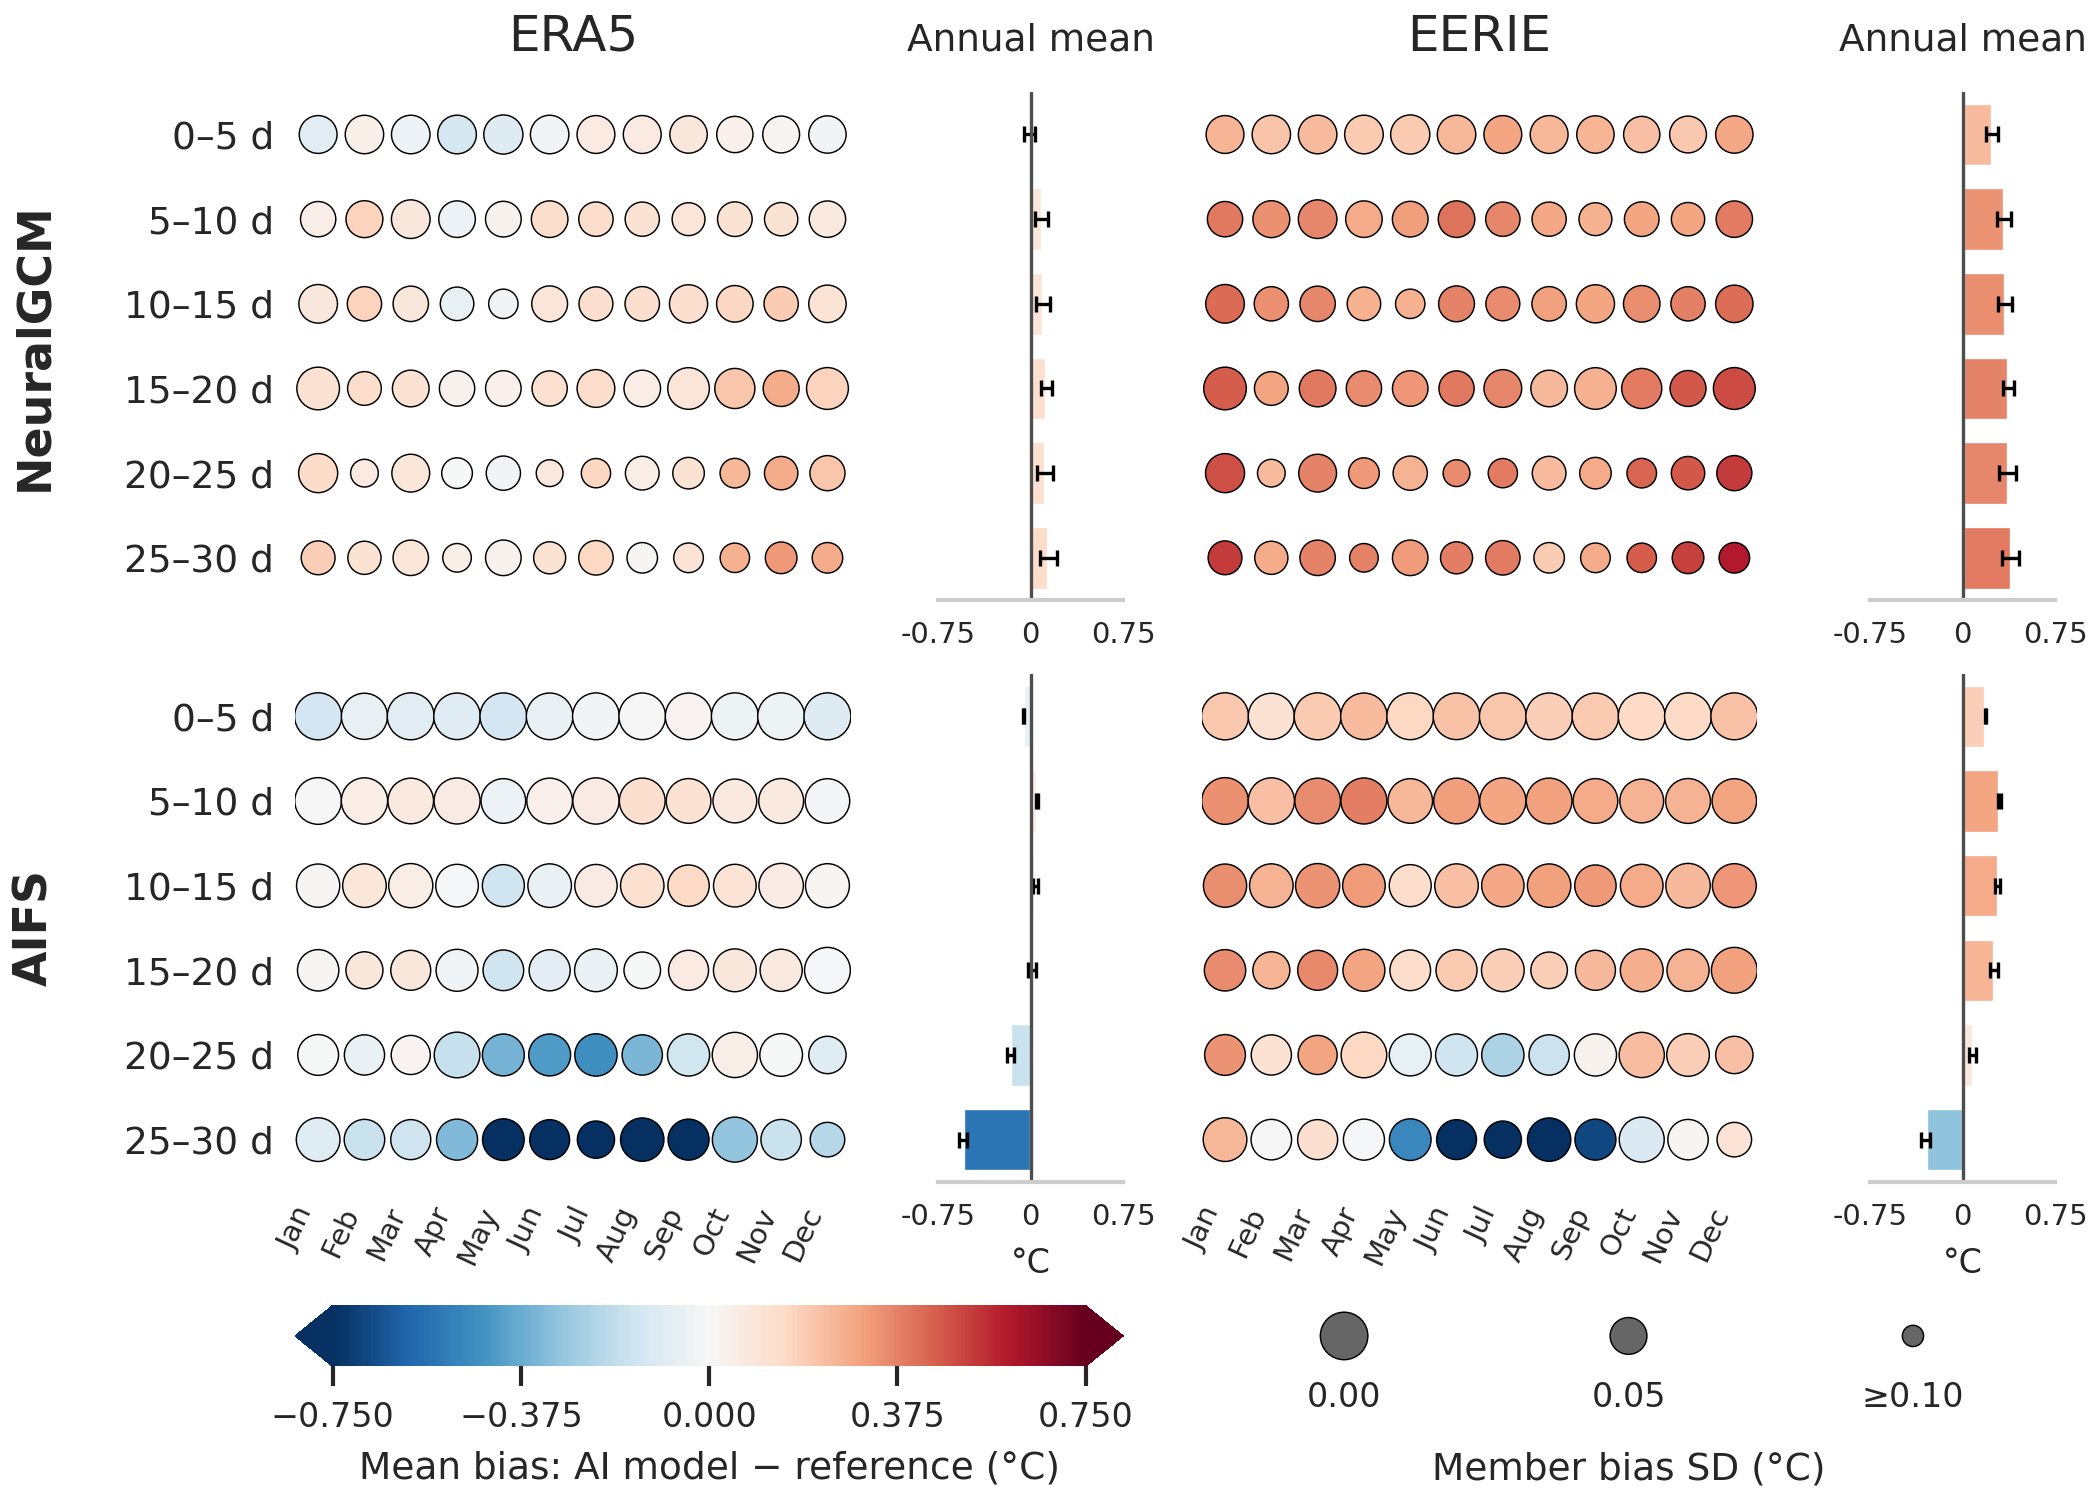
\includegraphics[width=1\linewidth]{Chapter2//Figs/climatologie_bias_vars.png}
    \caption{Climatological bias in global mean temperature at 850~hPa during 1985--1990. NeuralGCM (top) and AIFS-CRPS (bottom) each use ten-member ensembles initialized from EERIE-AMIP member~1. Columns show comparisons with ERA5 (left) and EERIE-AMIP member~1 (right). Circle colours represent the ensemble mean of the area-weighted global biases (AI model minus reference) for each month and five day lead-time window. Larger circles indicate a smaller inter-member standard deviation of the global bias. Horizontal bars show the equally weighted mean of the twelve monthly biases; error bars indicate $\pm$ the mean of the twelve monthly inter-member standard deviations.}
    \label{fig:climatology-bias}
\end{figure}

The initial movement towards an ERA5-like global mean is consistent with an adjustment towards conditions represented in the training data, although the present diagnostics do not establish its mechanism. Related behaviour was reported by \citet{rackow_robustness_2024}, who found that AI weather models could retain useful forecast skill when initialized in different climate states while developing systematic temperature drift towards their training climate. Their experiments concerned colder and warmer climate regimes, whereas the present comparison concerns two representations of the same historical period. Nevertheless, both illustrate why forecast skill and preservation of the source climate must be evaluated separately.

The spatial RMSE provides a further distinction between agreement in the global mean and agreement in the geographical temperature distribution (Figure~\ref{fig:climatology-rmse}). Relative to ERA5, NeuralGCM maintains an annual mean spatial RMSE of approximately $1.1$--$1.3\,^{\circ}\mathrm{C}$ across the forecast windows, despite its much smaller global mean bias. Relative to EERIE-AMIP, RMSE increases from approximately $0.7\,^{\circ}\mathrm{C}$ during days 0--5 to around $1.4\,^{\circ}\mathrm{C}$ during days 25--30. Thus, the relatively stable global mean does not imply preservation of the reference spatial climatology: regional differences remain substantial and can compensate when averaged globally.

AIFS-CRPS shows a broadly comparable spatial RMSE during the first 20 days, followed by a marked deterioration. During days 25--30, the annual mean RMSE reaches approximately $2.5\,^{\circ}\mathrm{C}$ relative to ERA5 and $2.7\,^{\circ}\mathrm{C}$ relative to EERIE-AMIP. The largest monthly errors occur during boreal summer and early autumn, matching the seasonal structure of the cold bias. These changes are much larger than the inter-member variation of the aggregated diagnostics, indicating that the deterioration is shared across the ensemble. 

The results therefore support the use of the 10--20-day interval as a pragmatic window for comparing the generated mean states, after the initial adjustment and before the strongest AIFS-CRPS deterioration. They do not demonstrate complete loss of initialization influence or convergence to an equilibrium climate. Published experiments have shown that selected NeuralGCM configurations can reproduce climate statistics in multi-decadal integrations \citep{kochkov_neural_2024}, while AIFS-CRPS has demonstrated skill in 46-day forecasts initialized from ERA5 \citep{lang_aifs-crps_2026}. These capabilities cannot be transferred automatically to a different initialization source. 

\begin{figure}[H]
    \centering
    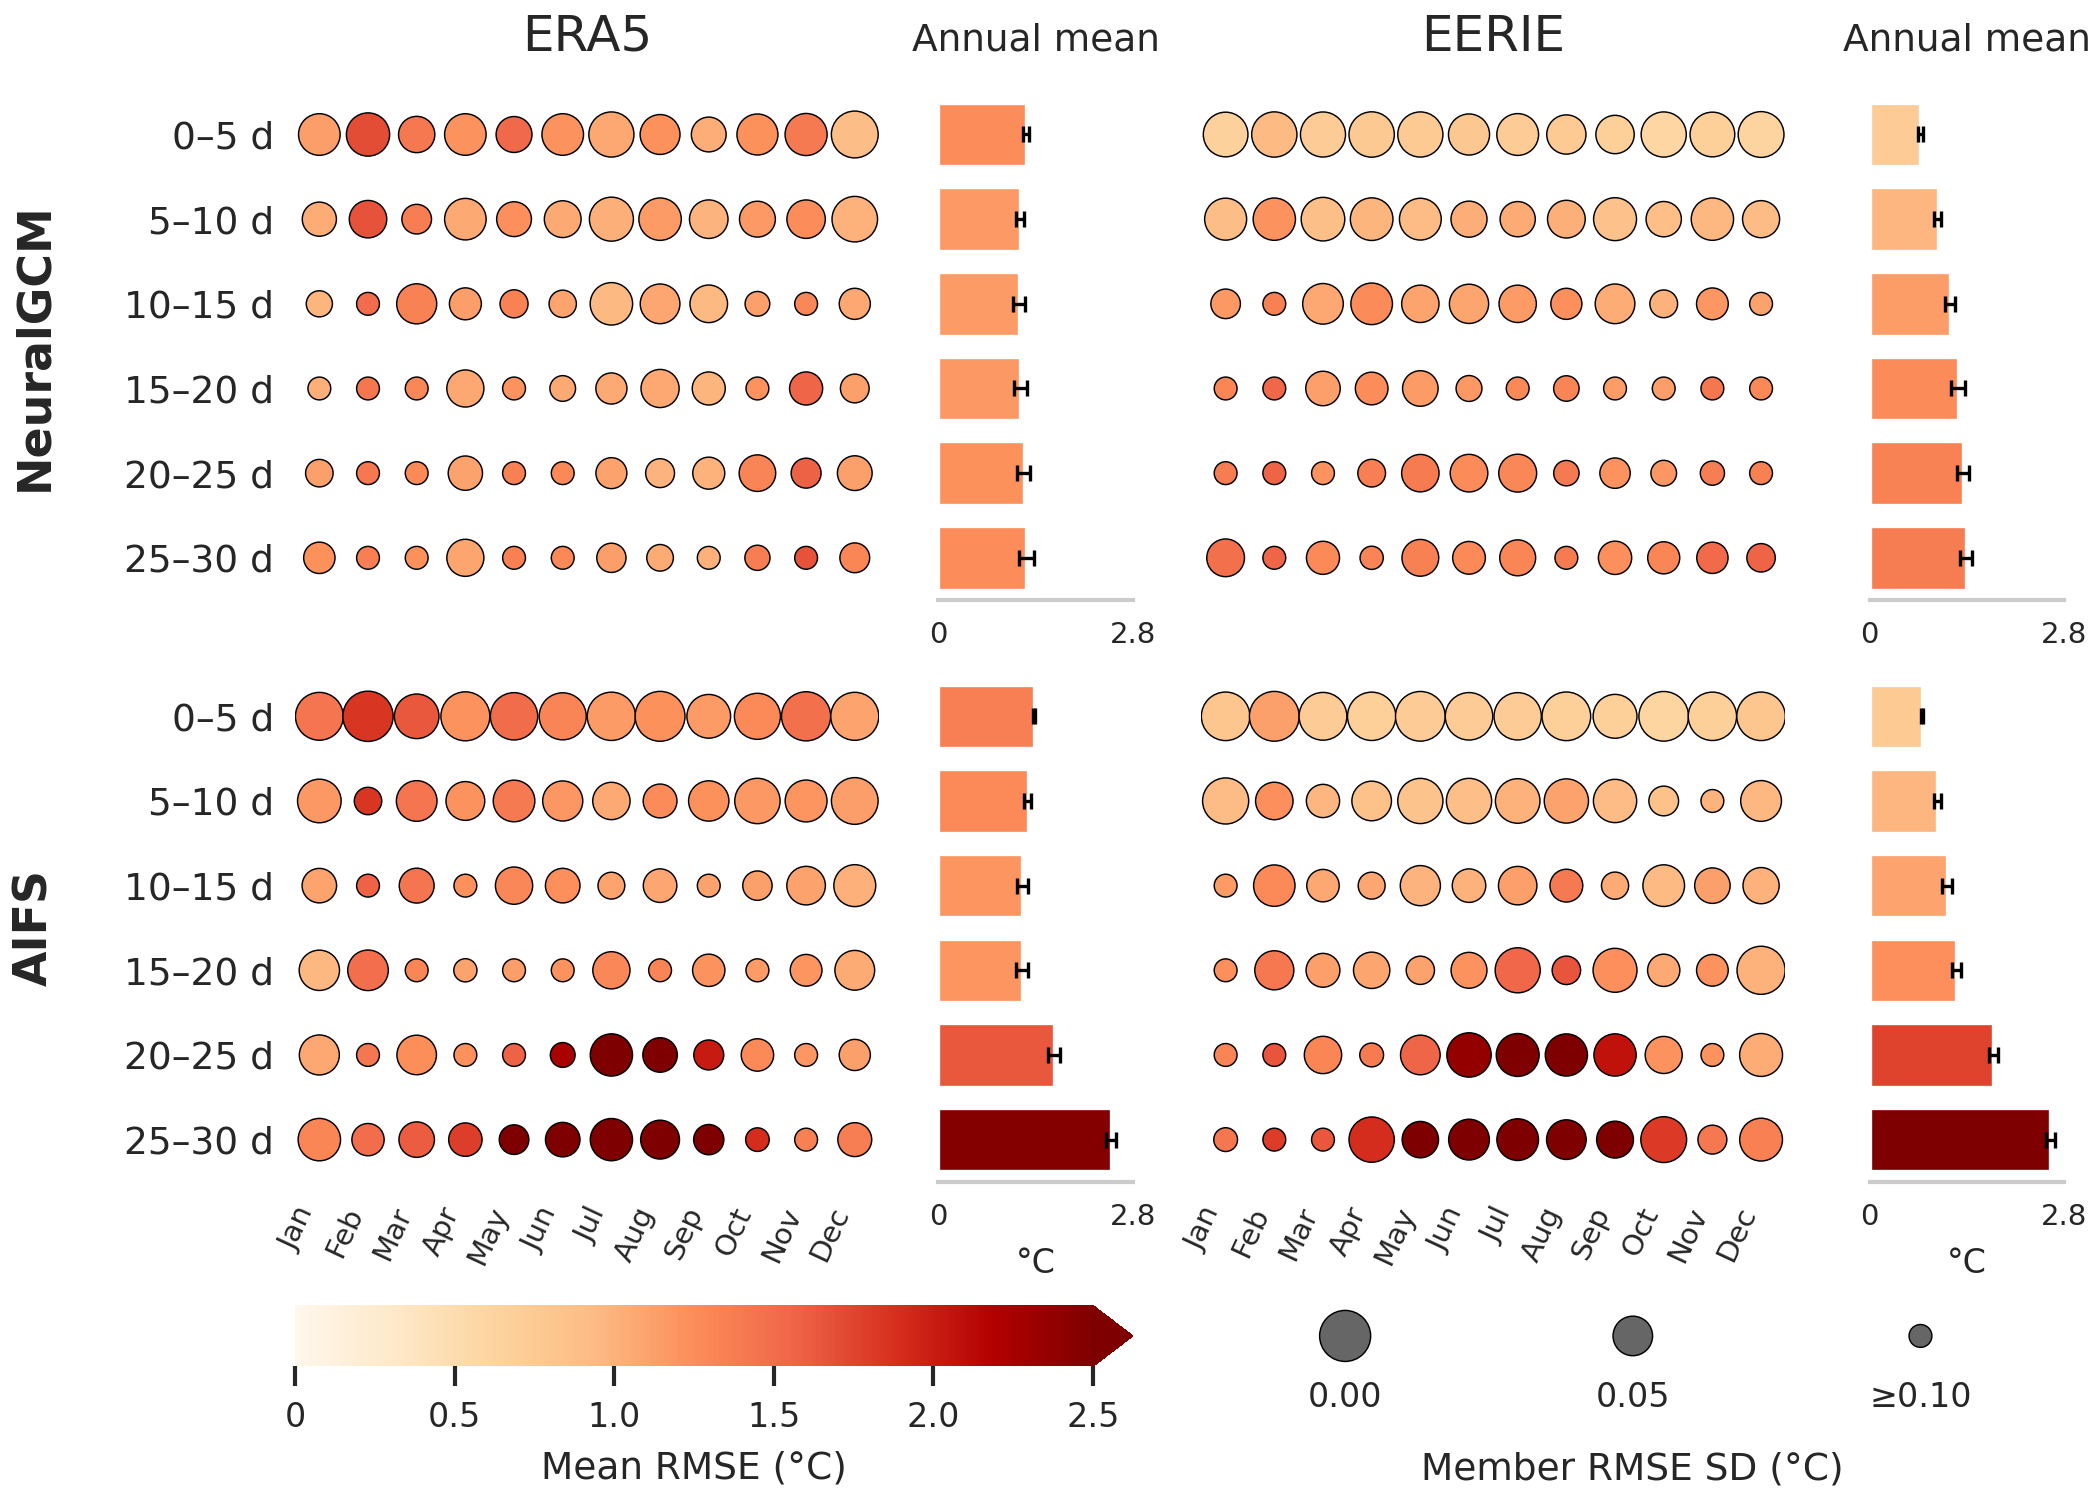
\includegraphics[width=1\linewidth]{Chapter2//Figs/climatologie_rmse_vars.png}
    \caption{Spatial RMSE of monthly climatological temperature fields at 850~hPa during 1985--1990. NeuralGCM (top) and AIFS-CRPS (bottom) each use ten-member ensembles initialized from EERIE-AMIP member~1. Columns show comparisons with ERA5 (left) and EERIE-AMIP member~1 (right). Circle colours represent the mean RMSE across ensemble members for each month and five-day lead-time window, with the spatial RMSE calculated separately for each member before averaging. Larger circles indicate a smaller inter-member standard deviation of the RMSE. Horizontal bars show the equally weighted mean of the twelve monthly RMSE values; error bars indicate $\pm$ the mean of the twelve monthly inter-member standard deviations.}
    \label{fig:climatology-rmse}
\end{figure}

\subsection{Anomalies and Variability}

\section{Discussion}
\chapter{Turning Climate Data into Information: Learning Meteorological Seasons}
\label{chap:climate-information}

\ifpdf
  \graphicspath{{Chapter3/Figs/}{Chapter3/Figs/PDF/}}
\else
  \graphicspath{{Chapter3/Figs/Vector/}{Chapter3/Figs/}}
\fi

\noindent\textit{Parts of this chapter are based on the work entitled \emph{A Machine Learning Framework for Objective Definition and Projection of Meteorological Seasons: an Application to the Indian Subcontinent}, by \textbf{Grassi, J.}, Palazzi, E., von Hardenberg, J., and Davini, P. The manuscript has been published in Journal of Geophysical Research: Atmospheres, a journal of the American Geophysical Union.}

\vspace{0.5em}
\begin{center}
    \rule{0.5\textwidth}{0.4pt}
\end{center}
\vspace{0.5em}

The previous chapter examined how AI-based weather forecasting models can contribute to the production of climate data. Access to abundant, reliable, and high-quality data is a non-negotiable prerequisite for effective Climate Services. However, it represents only the first step towards realizing their full potential. In practice, Climate Services have often prioritized the production and dissemination of increasingly detailed datasets while devoting less attention to the processes through which these data are interpreted, contextualized, and incorporated into decision-making \citep{findlater_climate_2021}.

As emphasized by the IPCC, observations and model outputs are not inherently decision-relevant: they become usable only when interpreted in relation to a specific purpose, spatial and temporal scale, and user context \citep[Sections~10.5.1--10.5.4]{doblas-reyes_linking_2021}. As also represented in the Climate Services value chain, the first step towards this goal is the extraction of information from data.

Borrowing the terminology used by the IPCC, turning climate data into useful information requires a process of \emph{distillation}. Within the DIKW framework adopted throughout this dissertation, the transformation from data to information occurs through two main processes: \emph{subsetting} and \emph{inference}. The same data can clearly form the basis for extracting very different types of information. Consider, for example, a time series of hourly temperature data. It can be used to estimate temperature extremes; when combined with precipitation data, it can inform drought indicators; and when wind data are also included, it can contribute to wildfire indicators. Even the same heat indicators may be computed differently depending on whether the objective is to investigate impacts on human health or on infrastructure operations.

In this context, the diagnostic capabilities of AI open a multitude of possible developments. AI algorithms can identify complex, nonlinear, and multivariate patterns in data that may be difficult to capture using conventional statistical or deterministic methods \citep{reichstein_deep_2019}. A comprehensive review of all the diagnostic AI algorithms developed in the Earth sciences is therefore beyond the scope of this dissertation. Here, we focus on a specific case and show how a simple Machine Learning algorithm, implementable in only a few lines of code, can extract useful information from large volumes of climate data and display a generalization capability that would be difficult to achieve using deterministic methods.

The specific case study concerns the identification of meteorological seasons in the Indian subcontinent. Most readers will have an intuitive understanding of what meteorological seasons are and why they are relevant to many aspects of our societies. At the same time, they may find it extremely difficult to translate this understanding into a sequence of deterministic instructions that can be supplied to an algorithm. This chapter shows how AI and ML can overcome this difficulty, translating such heuristic understanding into quantifiable indicators.


%********************************** % First Section  *************************************

\section{Meteorological Seasons as Climate Information}

Despite their apparent familiarity, seasons are difficult to define rigorously. Astronomical seasons divide the year according to equinoxes and solstices, whereas meteorological seasons are generally defined as fixed periods characterized by relatively homogeneous weather conditions. In temperate regions, for example, the year is conventionally divided into four three-month intervals corresponding to winter, spring, summer, and autumn \citep{trenberth_what_1983}. Such regularity, however, is rarely observed in the climate system. Seasonal transitions are gradual rather than discontinuous, and the timing and duration of individual climatic or ecological phases can vary considerably between years \citep{littleboy_worldseasons_2024}. The conventional four-season partition is also closely associated with the annual temperature cycle of the mid-latitudes and cannot be applied uniformly across the globe. In tropical regions, where annual temperature variability is limited, a distinction between wet and dry periods may provide a more meaningful representation of seasonality \citep{guo_regime_2022,bruijnzeel_overview_2005}. Polar regions are instead often characterized by a long cold season and a much shorter mild season \citep{serreze_arctic_2014}.

Against this background, climate change is already altering the timing and duration of seasonal cycles. Earlier spring and summer conditions, shorter winters, and shifts in traditional seasonal patterns have been observed in several regions \citep{woolway_pace_2023,sparks_observed_2002,morisette_tracking_2009,cayan_changes_2001}. These changes affect ecosystems \citep{ren_earlier_2024,uphus_earlier_2023}, agricultural production \citep{minoli_global_2022,tran_climate_2025}, water resources \citep{zhao_counteracting_2025}, and human health \citep{ruan_climate_2025,luthi_rapid_2023}. Their widespread impacts on human activities make the detection of changes in seasonality relevant not only for describing the climate system but also for understanding its evolving consequences.

These characteristics make meteorological seasons an example of climate information. They are not direct outputs of climate models but can be inferred from climate data. At the same time, they are not inherently decision-relevant on their own; they acquire meaning when contextualized within a specific setting, thereby contributing to the knowledge required for adaptation. The question is therefore: how can information about meteorological seasons be inferred from climate data, given their heuristic nature?

Conventional methods for identifying meteorological seasons generally rely on fixed calendar intervals or thresholds applied to one or more atmospheric variables \citep{kutta_reconsidering_2016,wang_changing_2021,hekmatzadeh_new_2020,de_la_franca_changes_2013}. These approaches are transparent and remain appropriate for many operational applications, particularly when the relevant variable and transition are already well defined. Their dependence on locally calibrated thresholds, however, can limit their transferability across regions, datasets, and climate conditions. A definition developed for a particular observational record may not be directly applicable to a climate model characterized by systematic biases or to future conditions that differ from those used to establish the original threshold.

AI and ML methods provide an alternative approach. Rather than prescribing in advance the atmospheric conditions associated with each season, they can identify groups of days or months characterized by similar multivariate states, through a clustering approach. Meteorological seasons can consequently be derived from the combined variability of temperature, precipitation, and atmospheric circulation, providing a multidimensional representation of the annual cycle \citep{chattopadhyay_predicting_2020,chidean_spatio-temporal_2020,lee_new_2023}. By maximizing similarity within clusters and separation between them, these methods reduce the need for variable-specific thresholds and allow seasonal boundaries to emerge from the structure of the data \citep{xu_clustering_2008}. Moreover, they can learn this seasonal representation and apply it to other datasets or model simulations allowing, for example, to quantify how the current seasons are expected to change in the next decades.

However, AI and ML do not work in the same dimensions as the ones of our understanding. The question that we have to pose ourselves is it then if the representation of the seasonal cycle produce by AI is meaningful also for our understanding, in such a way that the results obtained can be used as information underpinning the creation of decision-relevant knowledge. The value of this approach must therefore be assessed not only through statistical separation but also through physical interpretability and agreement with established climatic patterns.


\section{Case Study: The Indian Subcontinent}

To assess whether a data driven representation of seasons is both statistically robust and physically meaningful, the proposed framework is applied to the Indian subcontinent. The region provides a particularly relevant case study because its annual climate cycle is strongly pronounced but cannot be described adequately through the conventional sequence of temperate seasons. It also combines extensive climate data with established operational definitions of monsoon onset and withdrawal, providing an independent reference against which the inferred seasonal boundaries can be evaluated \citep{pai_normal_2020}. Finally, the timing and duration of its seasons have major implications for agriculture, water availability, ecosystems, and economic activities, making seasonality directly relevant to the provision of Climate Services.

The climate of the Indian subcontinent is primarily shaped by the South Asian monsoon system. During boreal summer, the seasonal contrast between the Asian landmass and the surrounding oceans drives a large-scale reorganization of atmospheric circulation. Moist southwesterly winds transport water vapour from the Arabian Sea and the Bay of Bengal towards the continent, producing the Indian Summer Monsoon (ISM). The monsoon generally reaches southwestern India first and subsequently progresses across the subcontinent. Between June and September, it provides most of the annual precipitation received by large parts of India and supports agricultural production, water-resource availability, and the livelihoods of a substantial part of the population \citep{gadgil_indian_2003,amrith_risk_2018}.

The monsoon does not begin or end simultaneously across the region. Its onset, spatial progression, and withdrawal occur over several weeks and are influenced by topography, land--atmosphere interactions, and large-scale circulation. The resulting transitions are therefore gradual and geographically heterogeneous. The India Meteorological Department (IMD) conventionally divides the annual cycle into four main periods: winter from December to February, pre-monsoon from March to May, monsoon from June to September, and post-monsoon from October to November \citep{praveen_analyzing_2020}. The IMD also provides a granular operative methods to establish the onset, progression, and withdrawal of the monsoon over the region \citep{pai_normal_2020}. 

Although the summer monsoon dominates much of the subcontinent, it is not the only circulation system determining regional seasonality. During winter, northern India and the surrounding mountain ranges are affected by Western Disturbances, extratropical weather systems embedded in the subtropical westerly jet \citep{pisharoty_western_1956}. These systems transport moisture towards the Hindu Kush, Karakoram, and Himalayan regions, producing rainfall at lower elevations and snowfall over the mountains. Winter precipitation contributes to the accumulation of the Himalayan snowpack and influences the seasonal availability of water in downstream river basins \citep{dimri_western_2015,hunt_western_2025}. Consequently, the northern mountain regions exhibit a seasonal cycle that differs substantially from the monsoon-dominated lowlands.

The analysis considers the domain between $5$--$40^\circ$N and $65$--$100^\circ$E and focuses on four subregions representing its main climatic contrasts (Figure \ref{fig:india_orography}). Southwest India ($74$--$78^\circ$E, $8$--$15^\circ$N) includes the area where the summer monsoon typically first reaches the Indian mainland. Central India ($75$--$85^\circ$E, $15.5$--$25.5^\circ$N) lies within the core monsoon region and is characterized by a strong and well-defined summer rainfall regime. The Himalayan region ($78$--$93^\circ$E, $25$--$32^\circ$N) combines monsoon influence with complex topography, while the Hindu Kush--Karakoram region ($71$--$78^\circ$E, $32$--$37^\circ$N) is more strongly affected by Western Disturbances and winter precipitation. Together, these regions provide a range of seasonal regimes with different dominant circulation processes.

\begin{figure}[H]
    \centering
    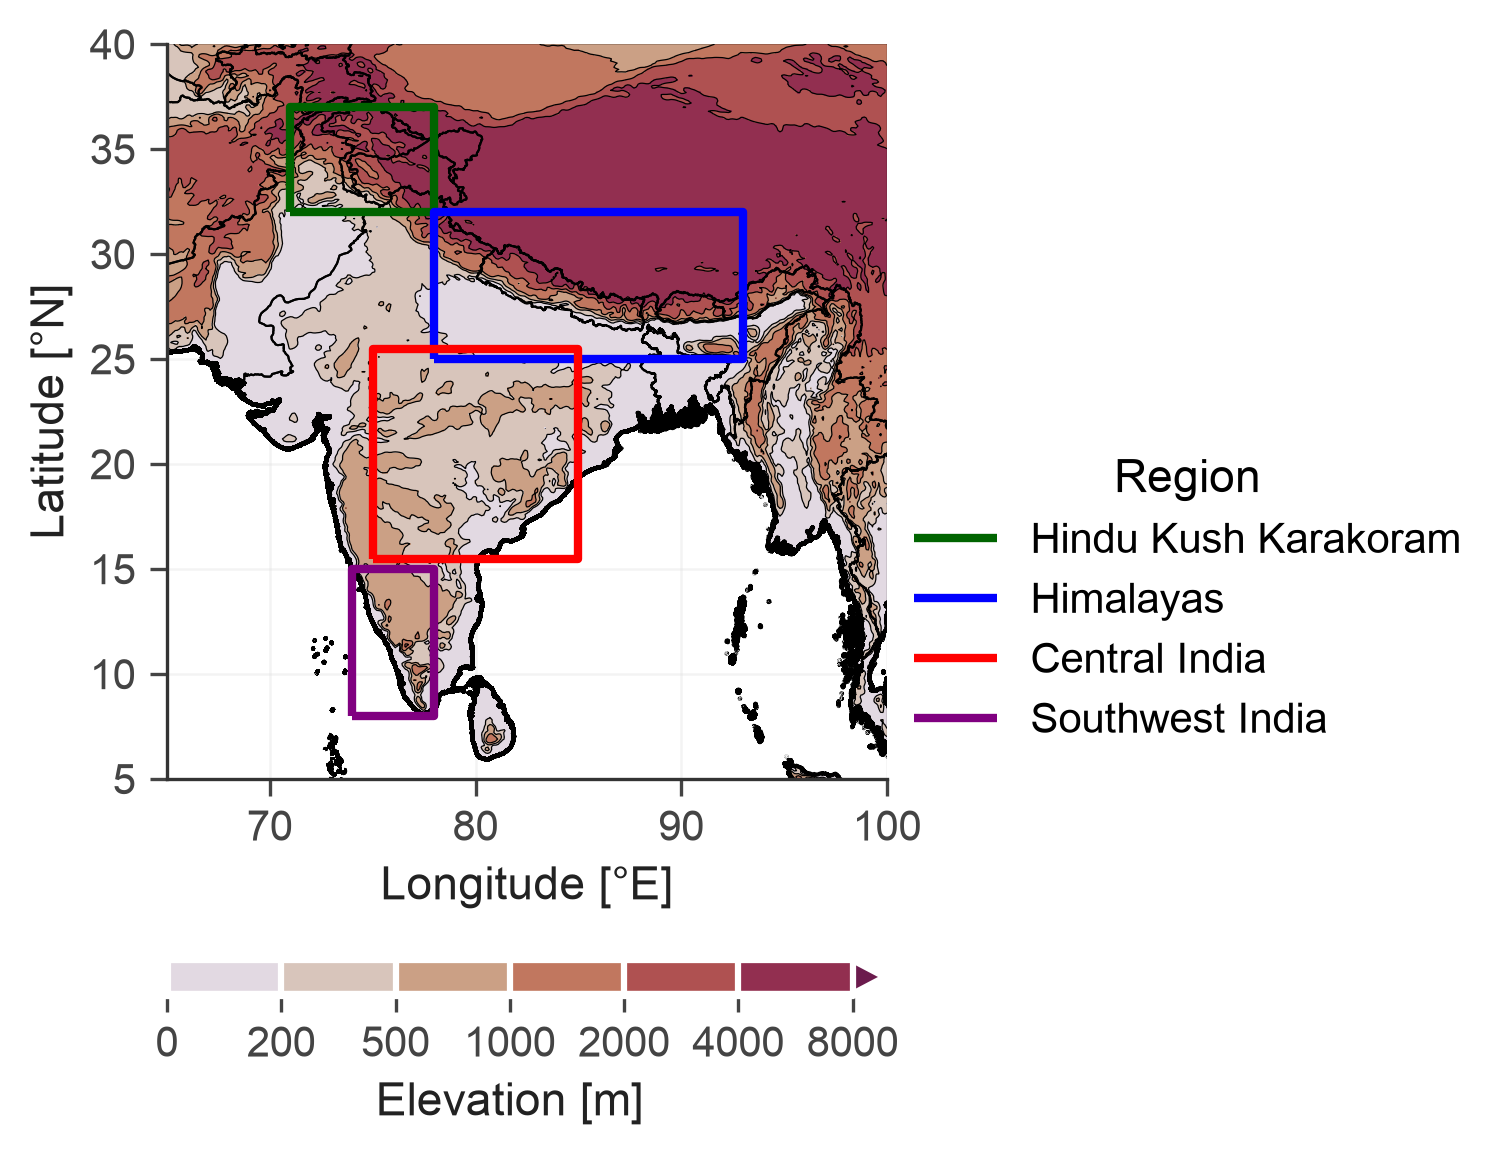
\includegraphics[width=0.75\linewidth]{Chapter3//figs/ERA5_orography_INDIA.png}
    \caption{Overview of the selected domain over the Indian subcontinent. 
    Orography is represented by shadings. 
    The four analyzed regions are highlighted by colored boxes.}
    \label{fig:india_orography}
\end{figure}

This climatic diversity makes the Indian subcontinent more than an illustrative application. In Central and Southwest India, the strong monsoon signal provides a relatively clear benchmark for evaluating whether the algorithm can identify established seasonal transitions. The Himalayan and Hindu Kush--Karakoram regions provide a more demanding test because of their complex topography and the interaction between summer and winter circulation systems. The case study therefore allows the framework to be evaluated under contrasting climatic conditions and makes it possible to assess whether a seasonal representation learned from climate data can be generalized without losing its physical meaning.

From a Climate Services perspective, the region also illustrates why seasonal information matters. Changes in monsoon onset or withdrawal can alter the timing of agricultural activities and water availability, while changes in the duration of winter can affect snowfall accumulation and downstream hydrology. A consistent method for identifying and tracking these seasonal phases can therefore transform multivariate climate data into indicators that are easier to compare across regions, models, and future periods.

\section{Data and Methods}

\subsection{Data}
We used both reanalysis and climate model simulations.
As reference, we employed ERA5 reanalysis daily data \citep{hersbach_era5_2020}, obtained from hourly outputs at original resolution (0.25° × 0.25°).
The variables considered are 2-meter temperature (tas), total precipitation (pr), and the zonal (ua850) and meridional (va850) wind components at 850 hPa.
These variables are among the most widely used in climatic characterization studies, as they jointly capture the main thermodynamic and dynamic components of the seasonal cycle. 

Reference values for the resulting seasonal transitions were compared with the most recent climatological normal onset and withdrawal dates of the Indian Summer Monsoon (ISM), as provided by the India Meteorological Department (IMD). The climatological normals correspond to the mean onset and withdrawal dates calculated over the period 1961–2019. These reference dates, available on a location-wise basis in \citet{pai_normal_2020}, were interpolated onto a 1° × 1° latitude–longitude grid using bilinear interpolation. The IMD dates are derived from a multi-step deterministic algorithm that combines precipitation thresholds with temporal continuity criteria. For a detailed description of this procedure, readers are referred to \citet{pai_normal_2020}.

To assess future changes, we analyzed a Coupled Model Intercomparison Project Phase 6 (CMIP6) Multi-Model Ensemble (MME), including both historical simulations (1961--2014) \citep{eyring_overview_2016} and future projections under the high-emission SSP5-8.5 scenario (2015--2100) \citep{oneill_scenario_2016}, using daily data. The ensemble includes one member for each different model to maximize model spread. 
The list of models used is reported in Table~\ref{tab:cmip6_models}.  

ERA5 and CMIP6 data underwent a common pre-processing pipeline.
First, all instances of 29\textsuperscript{th} February were removed to ensure a uniform 365-day calendar.
The data were then regridded to a common 1°~$\times$~1° latitude–longitude grid using bilinear interpolation to ensure spatial consistency across different native resolutions.
Finally, a 15-day centered rolling mean was applied to each variable to smooth high-frequency fluctuations and emphasize intra-seasonal variability relevant to the identification of meteorological seasons.

Since one of the goals of the analysis is to evaluate how seasonal patterns are represented in future projections, we additionally applied a common detrending and normalization procedure to both ERA5 and CMIP6 data in order to remove signals that could bias the detection. Specifically, for each variable and each grid point, standardized anomalies (z-scores) were computed within a 10-year moving window for every calendar day by subtracting the running mean and dividing by the corresponding running standard deviation. This normalization was therefore applied consistently across variables, spatial locations, and temporal windows in both datasets. The resulting standardized fields filter out low-frequency drifts, such as the gradual warming signal, and act as an effective debiasing procedure across models and periods, ensuring that the clustering and classification focus on the internal seasonal dynamics rather than on systematic model biases or long-term trends.

\subsection{Machine-Learning Framework}

To identify meteorological seasons in the current climate, to validate the capabilities of the models to reproduce them and to estimate their future evolution we adopted a two-step approach.  
First, we defined the baseline seasons from a set of multiple atmospheric variables using ERA5 reanalysis by applying an unsupervised temporal clustering algorithm.  
Second, we used a supervised classification model to extend this seasonal segmentation to the CMIP6 multi-model ensemble, both in present-day conditions and in future projections.  

In the first step, Radially Constrained Clustering (RCC; \citet{cannon_defining_2005}) was applied to identify temporally contiguous seasons.  
In the second step, a Multinomial Logistic Regression Classifier (MLRC; \citet{hastie_elements_2009}) was trained to learn the association between atmospheric states and the RCC-derived seasonal labels.  
Once trained, the MLRC was applied to classify each day in the CMIP6 MME.  
This framework allowed us to assess the ability of CMIP6 models to reproduce the seasonal cycle identified in ERA5 and to explore projected changes in seasonal characteristics over the 21\textsuperscript{st} century.

\subsubsection{Radially Constrained Clustering}
The Radially Constrained Clustering algorithm (RCC; \citet{cannon_defining_2005}) is used to define a number $k$ of seasons by their breakpoints $B=\{b_1, ... ,b_k\}$, i.e. the dates that mark the transition from one season to another.
In this study we set k = 4, corresponding to the four main phases of the  seasonal cycle in India : winter, pre-monsoon, monsoon, and post-monsoon. This choice was made to obtain a level of temporal granularity that is consistent with the commonly used seasonal description of the Indian climate and allows a direct comparison with existing literature and operational classifications. 

Differently with other widely used clustering algorithms that partition the data in the feature space (such as k-means \citep{lloyd_least_1982}), RCC ensures that the clusters are temporally disjoint. 
Furthermore, RCC treats the last day of the year as continuous to the first, allowing a season to span across the boundary between December $31^{st}$ and January $1^{st}$.

To run the clustering we considered, for each grid point, the four time series of tas, pr, ua850, and va850 from ERA5 for 59 years from 1961 to 2019. The temporal domain was chosen to align with the study by \citet{pai_normal_2020}, which defines the monsoon onset and withdrawal normal dates (i.e., the average onset and withdrawal date over the period 1961--2019). These dates were used as a reference for validating the results of the clustering in the present study. 

We reshaped the data into a design matrix $X$ with dimensions $365 \times 236$. Rows correspond to calendar days, while columns correspond to variable–year combinations. Since four variables (tas, pr, ua850, and va850) were considered over 59 years (1961--2019), the total number of features is $4 \times 59 = 236$. Thus, each column contains the 365--day annual cycle of one variable for one specific year. We then applied a min–max normalization independently to each feature to preserve the seasonal evolution and relative phasing of the variable throughout the year.

The clusters were then defined by the set $B$ of the $k$ breakpoints that minimizes the Within Clusters Sum of Squares (WCSS):

\begin{linenomath*}
    \begin{equation}
        WCSS = \sum_{i=1}^k \sum_{j \in c_i} \sum_{d \in D} \left( x_{j,d} - \mu_{i,d} \right)^2
    \end{equation}
\end{linenomath*}

where $x_{j,d}$ is the value of the feature $d \in D$ on day $j$, and $\mu_{i,d}$ is the mean value of feature $d$ within cluster $c_i$.

The minimum of the WCSS is searched through an iterative algorithm: 

\begin{enumerate}
    \item Generate a set $B$ of $k$ breakpoints equally spaced in the year.
    \item Update each breakpoint $b_i$ in $B$ by adding a random value drawn from $U(-\eta,\eta)$. In this work we set $\eta=3$.
    \item Compute WCSS over the design matrix $X$ using the updated breakpoints. 
    \item If WCSS decreases, retain the new breakpoints, otherwise, revert to the previous ones.
    \item Repeat steps 2-4 for a predefined number of iterations.
\end{enumerate}

\subsubsection{Multinomial Logistic Regression Classifier}

To project the seasons defined on ERA5 with RCC onto each climate model from CMIP6, we employed a Multinomial Logistic Regression Classifier (MLRC; \citet{hastie_elements_2009}). 
For each day, the MLRC estimates the probability of belonging to each season $k \in \{1,\dots,K\}$ using the SoftMax function:

\begin{linenomath*}
    \begin{equation}
        p_{i,k} = \frac{\exp(\mathbf{w}_k\cdot\mathbf{x}_i)}{\sum_{j=1}^{K} \exp(\mathbf{w}_j\cdot\mathbf{x}_i)}
    \end{equation}
\end{linenomath*}

where $\mathbf{x}_i$ is the vector of predictors (precipitation, near-surface air temperature, and zonal and meridional wind components), $\mathbf{w}_k$ is the weight vector for class $k$, and $p_{i,k}$ is the estimated probability that day $i$ belongs to season $k$.

The model parameters $\mathbf{w}$ are optimized by minimizing the categorical cross-entropy loss over $N$ samples:

\begin{linenomath*}
    \begin{equation}
        L = -\frac{1}{N} \sum_{i=1}^{N} \sum_{k=1}^{K} y_{i,k} \, \log(p_{i,k})
    \end{equation}
\end{linenomath*}

where $y_{i,k}$ is a binary indicator equal to 1 if sample $i$ belongs to season $k$, and 0 otherwise. 
The optimization is performed over multiple epochs using the Adam algorithm \citep{kingma_adam_2017}.

We trained the MLRC on ERA5 daily data for the period 1961--2009, using the seasons identified by the RCC as categorical labels. An independent MLRC was trained at each grid point, and the resulting pointwise classifications and coefficients were subsequently aggregated over the four representative regions. As predictors, we used the same four atmospheric variables employed in the clustering step (tas, pr, ua850, va850), thus ensuring full consistency between the unsupervised and supervised phases of the framework.
As predictors, we used the same four atmospheric variables employed in the clustering step (tas, pr, ua850, va850) thus ensuring full consistency between the unsupervised and supervised phases of the framework.
The training dataset comprised 17,885 daily samples, which were divided into batches of size 52, and the model was trained over 100 epochs.

Since the MLRC is based on a linear decision function, the learned coefficients provide a direct interpretation of the influence of each predictor on the seasonal classification \cite{hastie_elements_2009}. To compare the relative role of the different predictors, we quantified their importance from the normalized magnitude of the class-specific coefficients:
\begin{equation}
I_{m,k} =
\frac{|w_{m,k}|}
{\sum_{m=1}^{M}|w_{m,k}|}
\times 100 (\%),
\end{equation}
where $w_{m,k}$ denotes the coefficient associated with predictor $m$ in the weight vector $\mathbf{w}_k$. By construction, the resulting importance values sum to 100\% for each season and grid point, providing an interpretable measure of the relative contribution of temperature, precipitation, zonal wind, and meridional wind to the classification.

\subsubsection{Validation and skill}

To assess the capability of the CMIP6 MME to reproduce the seasonal cycle and the effectiveness of our classification algorithm in identifying the correct season, we classified each day of each model for the period that overlaps ERA5 (1961-2015), and we computed the $F1$ Score \cite{blair_information_1979} for each model and season across the four spatial boxes (Figure \ref{fig:india_orography}). 

To provide an out-of-sample reference for classifier performance, the trained MLRCs were also applied to the held-out ERA5 period 2010--2019, and the resulting F1 scores were computed against the RCC-derived seasonal labels.


$F1$ score is the harmonic mean of precision and recall, and it is defined as:

\begin{linenomath*}
    \begin{equation}
        F1=2*\frac{precision*recall}{precision+recall}
    \end{equation}
\end{linenomath*}

where the precision measures the fraction of days classified in the season $x$ that actually belong to season $x$, and the recall the fraction of days classified in the season $x$ over the total number of days in the season $x$:

\begin{linenomath*}
    \begin{equation}
            precision = \frac{True\ positive}{True\ positive + False\ positive}\\
    \end{equation}
\end{linenomath*}

\begin{linenomath*}
    \begin{equation}
            recall = \frac{True\ positive}{True\ positive + False\ negative}
    \end{equation}
\end{linenomath*}

Values of $F1$ range from 0 to 1, with higher scores indicating better agreement between the predicted and reference seasonal labels. 
A value close to 1 denotes high classification accuracy, meaning that most days are correctly assigned to their corresponding season. 
In the present four-class problem, a random assignment would yield an expected $F1$ of approximately 0.25. 
Therefore, values around 0.5 indicate that the model performs roughly twice as well as random guessing, representing a threshold between poor and moderate skill. 
In this study, we adopt $F1 = 0.7$ as a practical threshold for good performance. 
From the definition in Eq. 4, this value implies that neither precision nor recall can fall below 0.5 unless the other is very high (e.g., $P = 0.9$ if $R = 0.5$). 
Hence, setting the threshold at 0.7 ensures that both metrics are simultaneously satisfactory, balancing detection capability and false alarm rate.

\section{Results}

\subsection{Meteorological Seasons from Reanalysis Data}

The first step of the framework consists of allowing the RCC algorithm to learn the meteorological seasons from ERA5 reanalysis data. We applied the algorithm to every grid point within the study domain and then aggregated the resulting seasonal breakpoints by averaging them over the four subregions shown in Figure~\ref{fig:india_orography}. We then assessed whether the seasonal partition identified by the RCC was consistent with the operational classification adopted by the IMD. The aim was to determine whether, beyond the mathematical consistency of the clustering, the resulting seasons corresponded to established operational definitions and could therefore provide meaningful information for real world applications.

We found that the clustering identifies four distinct seasons that closely reproduce the partitioning adopted by the IMD: monsoon (June--September), post-monsoon (October--November), winter (December--February), and pre-monsoon (March--May) \citep{praveen_analyzing_2020}, as shown in Figure~\ref{fig:clustering_results_polar}.  
The timing of monsoon onset and withdrawal aligns well with the IMD-defined phases of the Indian Summer Monsoon (ISM) \cite{pai_normal_2020}, with the onset in Southwest India (blue line) occurring earlier than in other regions, in agreement with the climatological progression of the monsoon (Figure~\ref{fig:clustering_results_polar}).  

For the other three seasons, whose boundaries are not as clearly defined in the literature, the clustering still provides a coherent segmentation (Figure~\ref{fig:clustering_results_polar}).  
The main discrepancy with the IMD subdivision emerges in the transition from winter to pre-monsoon, where the algorithm identifies a boundary that extends further into pre-monsoon.  
This behavior is more consistent with the definition of the Western Disturbance season proposed by \citet{palazzi_precipitation_2013}, spanning from December to April. Indeed the Hindu Kush-- Karakoram (yellow line) region is the one which present a longer winter season duration.  (Figure~\ref{fig:clustering_results_polar}). 

\begin{figure}[H]
    \centering
    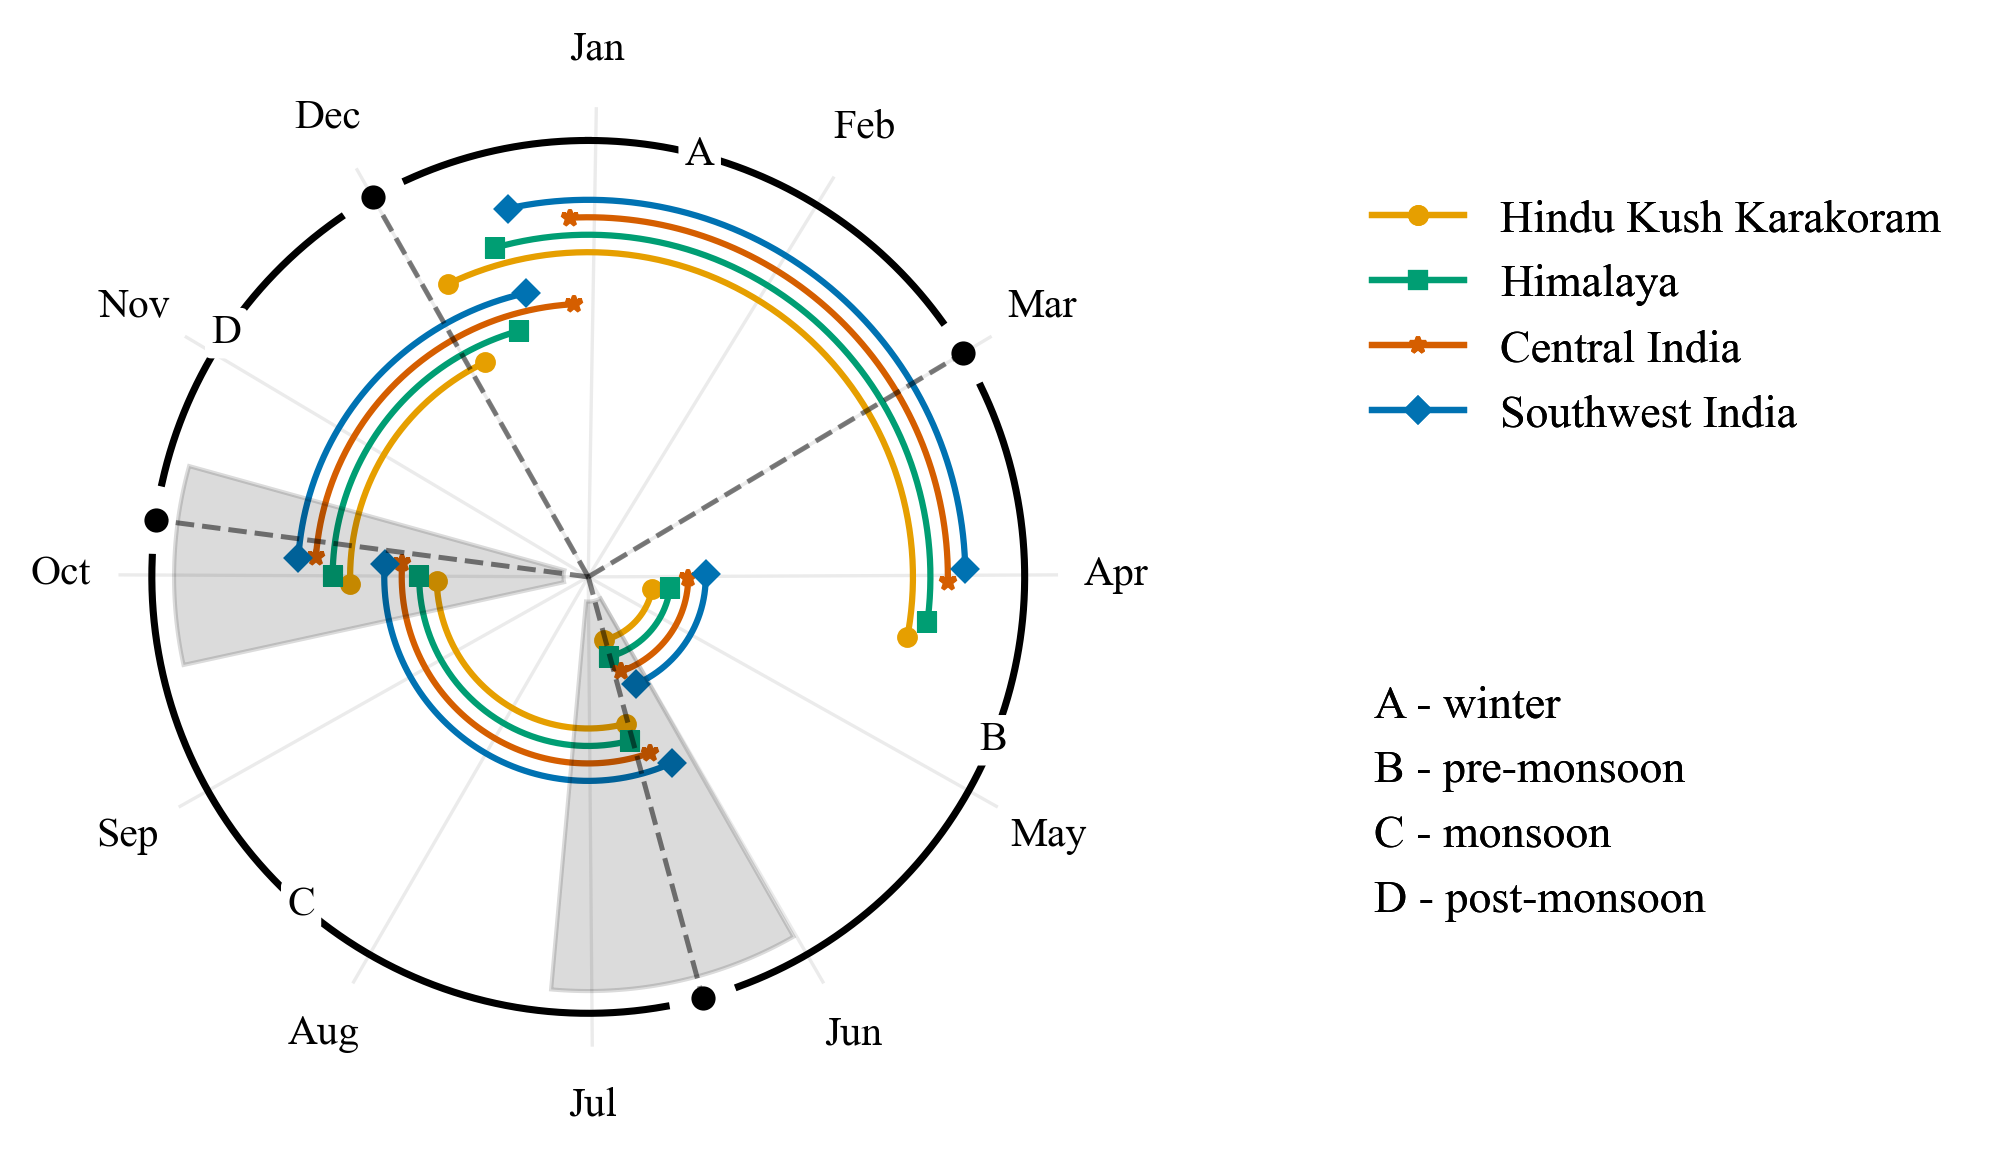
\includegraphics[width=0.8\textwidth]{Chapter3/figs/clustering_results_polar_coverage_all_regions.png}
        \caption{Seasonal coverage for the four focus regions. 
        Each colored arc corresponds to the median duration of the four identified seasons 
        (pre-monsoon, monsoon, post-monsoon, and winter), estimated from RCC clustering.
        The black outer reference ring highlights the subdivision adopted by the India Meteorological Department (IMD). 
        The shaded grey sectors around the monsoon onset and withdrawal represent the spatial variability (i.e., minimum and maximum dates) of IMD onset and withdrawal across India. 
        The monsoon onset and withdrawal medians are derived from \cite{pai_normal_2020}, using the normal onset and withdrawal dates averaged across the entire Indian landmass. 
        Month labels (e.g., ``Feb'') indicate the first day of each month, following a clockwise chronological order starting from January.}
        
    \label{fig:clustering_results_polar}
\end{figure}


Beyond the qualitative comparison, we also compared the identified breakpoints with the official monsoon onset and withdrawal normal dates provided by the IMD for each grid point over India. The RCC-derived monsoon onset is broadly consistent with the IMD climatology, although non-negligible regional differences are present. Positive differences occur in the southeastern part of the domain, corresponding to Andhra Pradesh, and in the northern part, corresponding to Ladakh, whereas negative differences are found in the northwestern part, particularly over Punjab and Rajasthan (see Figure \ref{fig:clustering_bias}a). 
A point-wise comparison of onset dates (Figure \ref{fig:clustering_dispersion}a) indicates that RCC tends to anticipate the advance of the monsoon relative to the IMD normals. 
The linear fit between the IMD reference dates (x-axis) and the RCC-derived dates (y-axis) yields a slope m=0.39, indicating that the spatial progression detected by RCC is more compressed in time than in the IMD reference. 
The spatial correspondence between the two fields is moderate, with a Pearson correlation coefficient r=0.35.

For monsoon withdrawal, the RCC--IMD differences are overall slightly positive, except over the southwestern part of the peninsula, where RCC identifies an earlier transition (Figure \ref{fig:clustering_bias}b). 
The point-wise comparison (Figure \ref{fig:clustering_dispersion}b) shows that RCC defines a slightly faster withdrawal progression (m=0.77), largely driven by the negative differences over the southern peninsula. The spatial correspondence is higher than for onset, with r=0.53. 
This result should nevertheless be interpreted cautiously, since the monsoon withdrawal has been less explored than the onset \citet{pai_normal_2020}, and its assessment remains challenging because of the larger interannual variability \citet{syroka_withdrawal_2004}.

\begin{figure}[H]
    \centering
    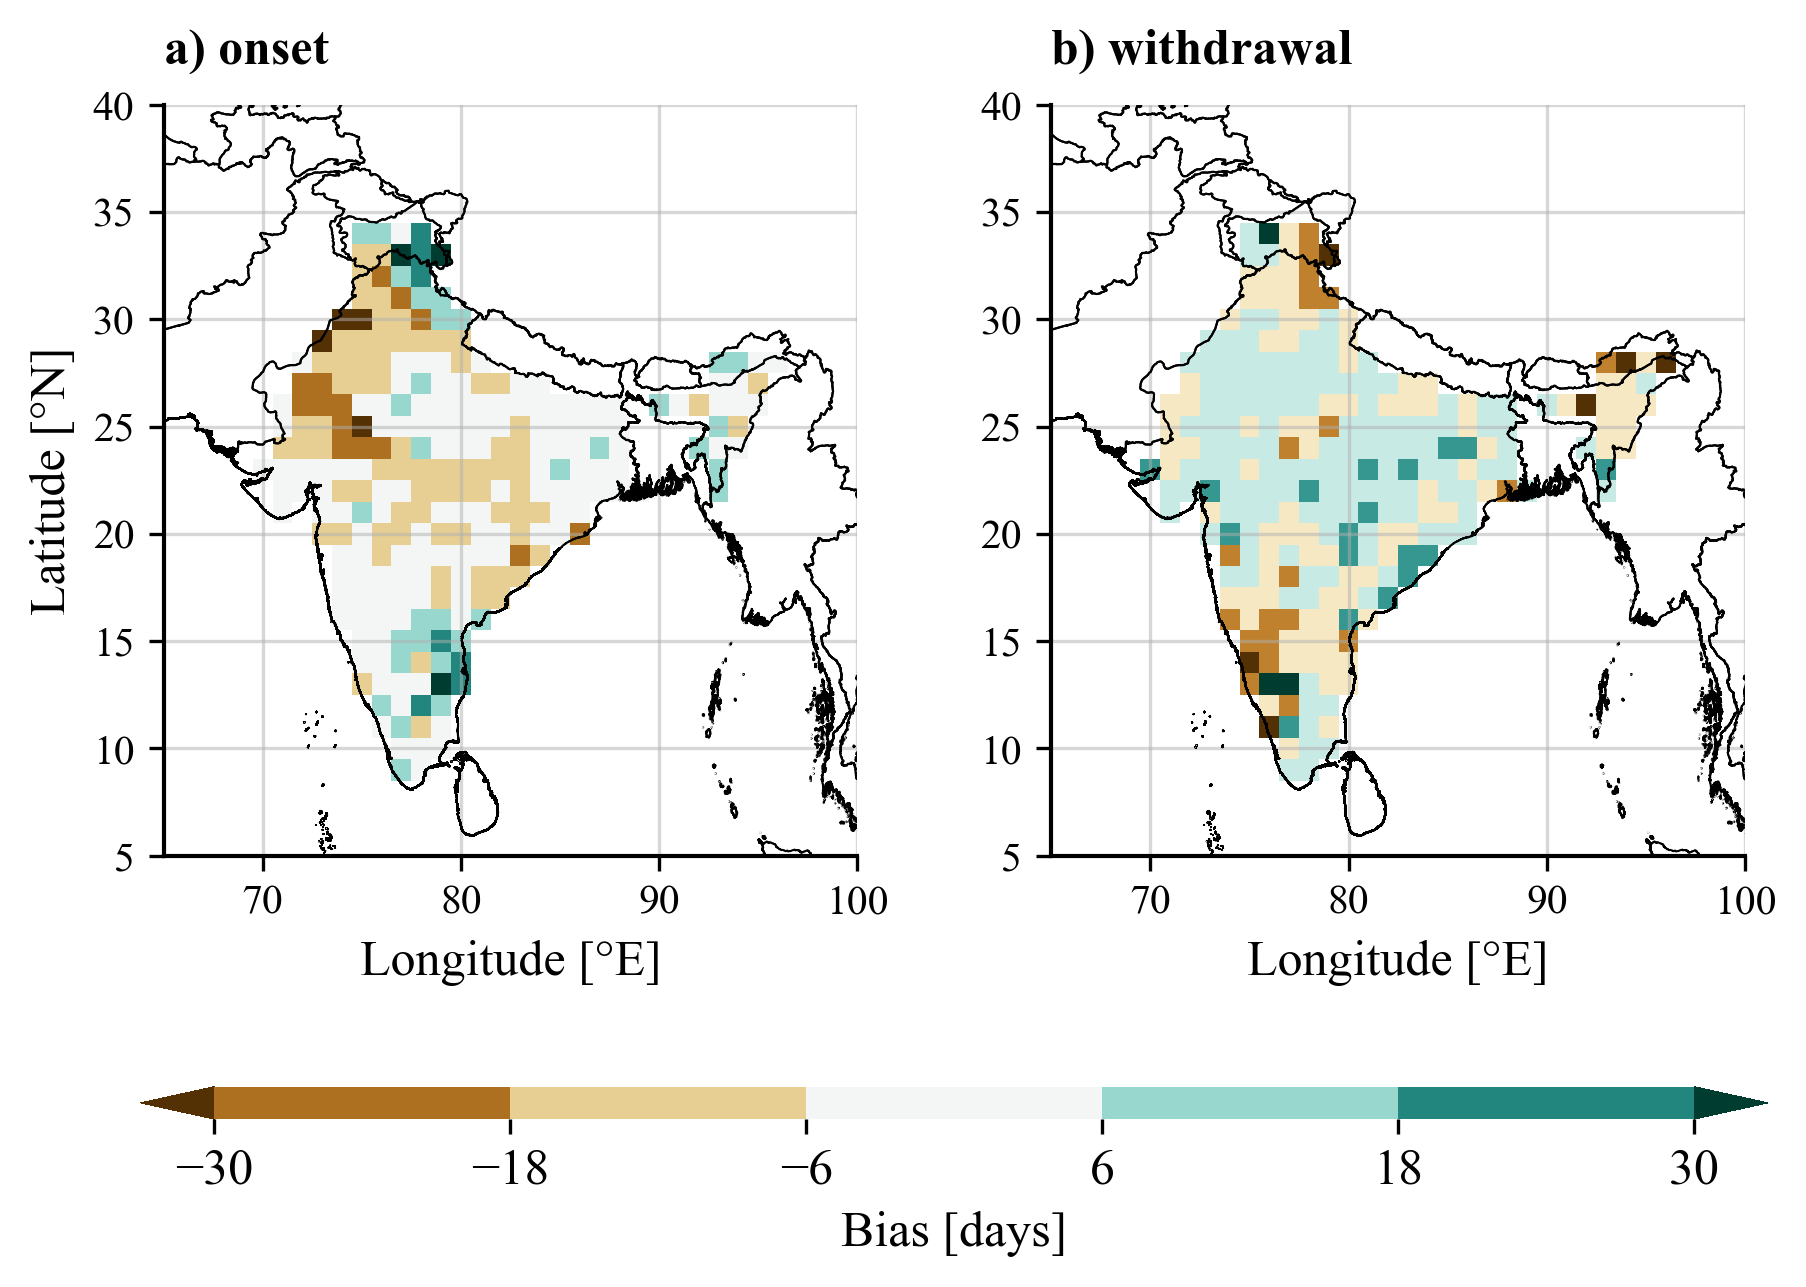
\includegraphics[width=0.7\textwidth]{Chapter3/figs/clustering_bias.png}
    \caption{Differences between the ISM phases by the RCC algorithm, compared to the reference dates provided by the IMD. Panel a shows the difference in monsoon onset dates between the RCC output and the IMD-defined climatological onset, while Panel b shows the difference in withdrawal dates. Positive values indicate a later transition identified by the RCC, and negative values an earlier one. Both fields are clipped over the IMD reference domain.}
    \label{fig:clustering_bias}
\end{figure}

\begin{figure}[H]
    \centering
    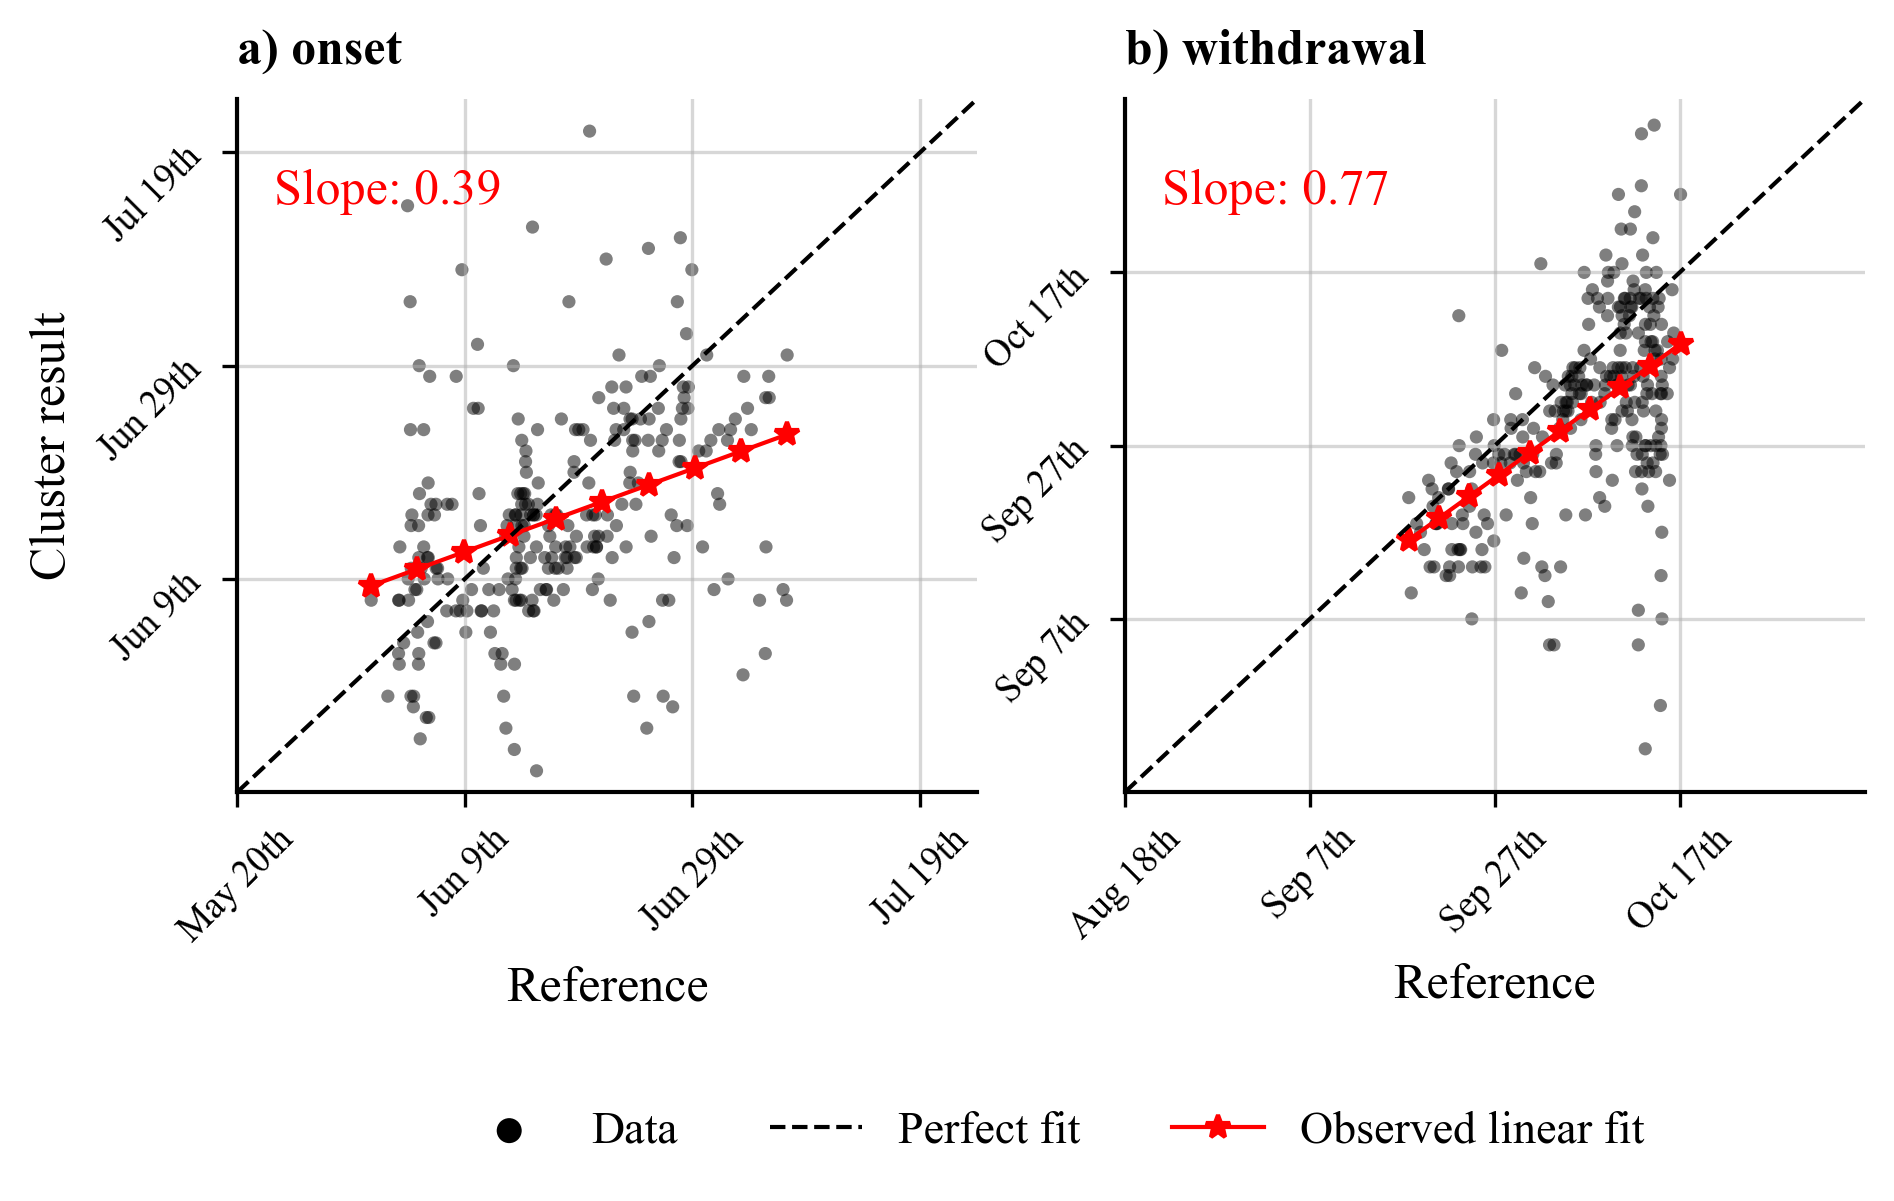
\includegraphics[width=0.7\textwidth]{Chapter3/figs/clustering_dispersion.png}
    \caption{Scatter plots comparing the seasonal transition dates identified by the RCC algorithm with the climatological reference dates from the IMD, across all grid points over the Indian subcontinent. Panel A shows the comparison for the monsoon onset, while Panel B refers to the monsoon withdrawal. Each point represents a single grid cell, with the reference date on the x-axis and the corresponding RCC-based date on the y-axis. The black dashed line indicates perfect agreement (1:1 line), while the red dashed line shows the linear regression fit. The slope of the fit is reported in each panel: slope weaker than 1 implies that the onset/withdraw of the monsoon system is progressing in space at a faster pace than in the IMD dataset.}
    \label{fig:clustering_dispersion}
\end{figure}

These discrepancies are expected given the different methodologies and data employed in defining and detecting monsoon transitions.
They reflect both dataset dependence and the fact that the two approaches diagnose related, but not identical, quantities.
IMD uses different criteria and data from multiple sources for defining the onset and withdrawal of the monsoon, while the RCC method identifies transitions between multivariate seasonal regimes using temperature, precipitation, and 850 hPa winds from ERA5 reanalysis only.
Accordingly, the RCC breakpoints should be interpreted as the onset and decay of a multivariate monsoon-like regime, rather than as precipitation-only onset or withdrawal dates.
Furthermore, while some studies have attempted to evaluate the reliability of ERA5 in reproducing regional precipitation patterns \citep{paul_spatial_2024, singh_assessment_2021}, the present comparison should not be read as an assessment of the ability of ERA5 to reproduce IMD transition dates, but as a benchmark of consistency for the multivariate seasonal segmentation.

Also considering these difference between approaches, it is clear that the RCC is able to produce a meaningful representation of the seasonal partition. In the next sections we will explore how this partition can be transferred to CMIP6 models, allowing an evaluation of the future expected changes.  

\subsection{Physical Intepretation}
Before applying the trained MLRC to the CMIP6 ensemble, we analyzed the relative importance of the model predictors in order to provide an interpretation of the classification framework. Using the normalized magnitude of the regression coefficients we quantified the contribution of temperature, precipitation, zonal wind, and meridional wind to the identification of each season. The resulting feature importance values are summarized in Table~\ref{tab:feature_importance}. The relative importance of the MLRC predictors varies substantially across seasons and regions.  Temperature is the dominant predictor during the pre-monsoon season in all four regions, accounting for 39--56\% of the total importance. Winter classification shows a stronger regional dependence, with temperature contributing most in HKK and the Himalaya (43--44\%), while precipitation becomes the leading predictor in Central and Southwest India (32--44\%). During the monsoon season, precipitation is the dominant predictor in the Himalaya and Central India (31--49\%), whereas zonal wind contributes most in Southwest India (39\%). Post-monsoon classification is characterized by a larger contribution from circulation-related variables, with zonal wind emerging as the dominant predictor in Central and Southwest India (36--40\%). Overall, the results indicate that the relative importance of the predictors is season- and region-dependent, with no single variable dominating the classification across all conditions.

\begin{table}[H]
\centering
\caption{Relative importance (\%) of the MLRC predictors. The dominant predictor for each season and region is shown in bold and underlined.}
\begin{tabular}{llcccc}
\hline
Season & Variable & HKK & Himalaya & Central India & Southwest India \\
\hline

winter
& tas   & \underline{\textbf{44}} & \underline{\textbf{43}} & 19 & 10 \\
& pr & 19 & 16 & \underline{\textbf{32}} & \underline{\textbf{44}} \\
& ua850          & 20 & 29 & 30 & 26 \\
& va850          & 17 & 13 & 19 & 21 \\
\hline

pre-monsoon
& tas   & \underline{\textbf{39}} & \underline{\textbf{42}} & \underline{\textbf{56}} & \underline{\textbf{45}} \\
& pr & 15 & 16 & 18 & 20 \\
& ua850          & 23 & 22 & 14 & 21 \\
& va850          & 23 & 20 & 13 & 14 \\
\hline

monsoon
& tas   & \underline{\textbf{38}} & 23 & 15 & 29 \\
& pr & 17 & \underline{\textbf{31}} & \underline{\textbf{49}} & 18 \\
& ua850          & 23 & 30 & 18 & \underline{\textbf{39}} \\
& va850          & 22 & 17 & 17 & 13 \\
\hline

post-monsoon
& tas   & \underline{\textbf{31}} & 15 & 30 & 29 \\
& pr & 30 & \underline{\textbf{36}} & 17 & 20 \\
& ua850          & 20 & 27 & \underline{\textbf{40}} & \underline{\textbf{36}} \\
& va850          & 19 & 22 & 14 & 14 \\
\hline

\end{tabular}
\label{tab:feature_importance}
\end{table}


\subsection{Transferring Seasonal Definitions to Climate Models}

The next step was to determine whether the seasonal definitions learned from ERA5 could be transferred meaningfully to climate model simulations. We therefore applied the trained MLRC to the historical simulations of the CMIP6 multi-model ensemble for the period 1961--2015. This evaluation is important because a statistically coherent definition derived from reanalysis data does not necessarily remain valid when applied to models characterized by different biases and representations of regional climate processes.

Figure~\ref{fig:f1_scores} summarizes the agreement between the ERA5-derived seasonal definitions and the classifications obtained from CMIP6. The figure also reports the performance of the classifier over the held-out ERA5 period 2010--2019. The ERA5 results provide a reference for interpreting the CMIP6 scores: when performance is high over ERA5 but lower over CMIP6, the difference is likely related to the representation of the seasonal cycle in the climate models. Conversely, low scores in both datasets suggest that the seasonal regimes themselves are less clearly distinguishable using the selected variables and classifier.

\begin{figure}[H]
\centering
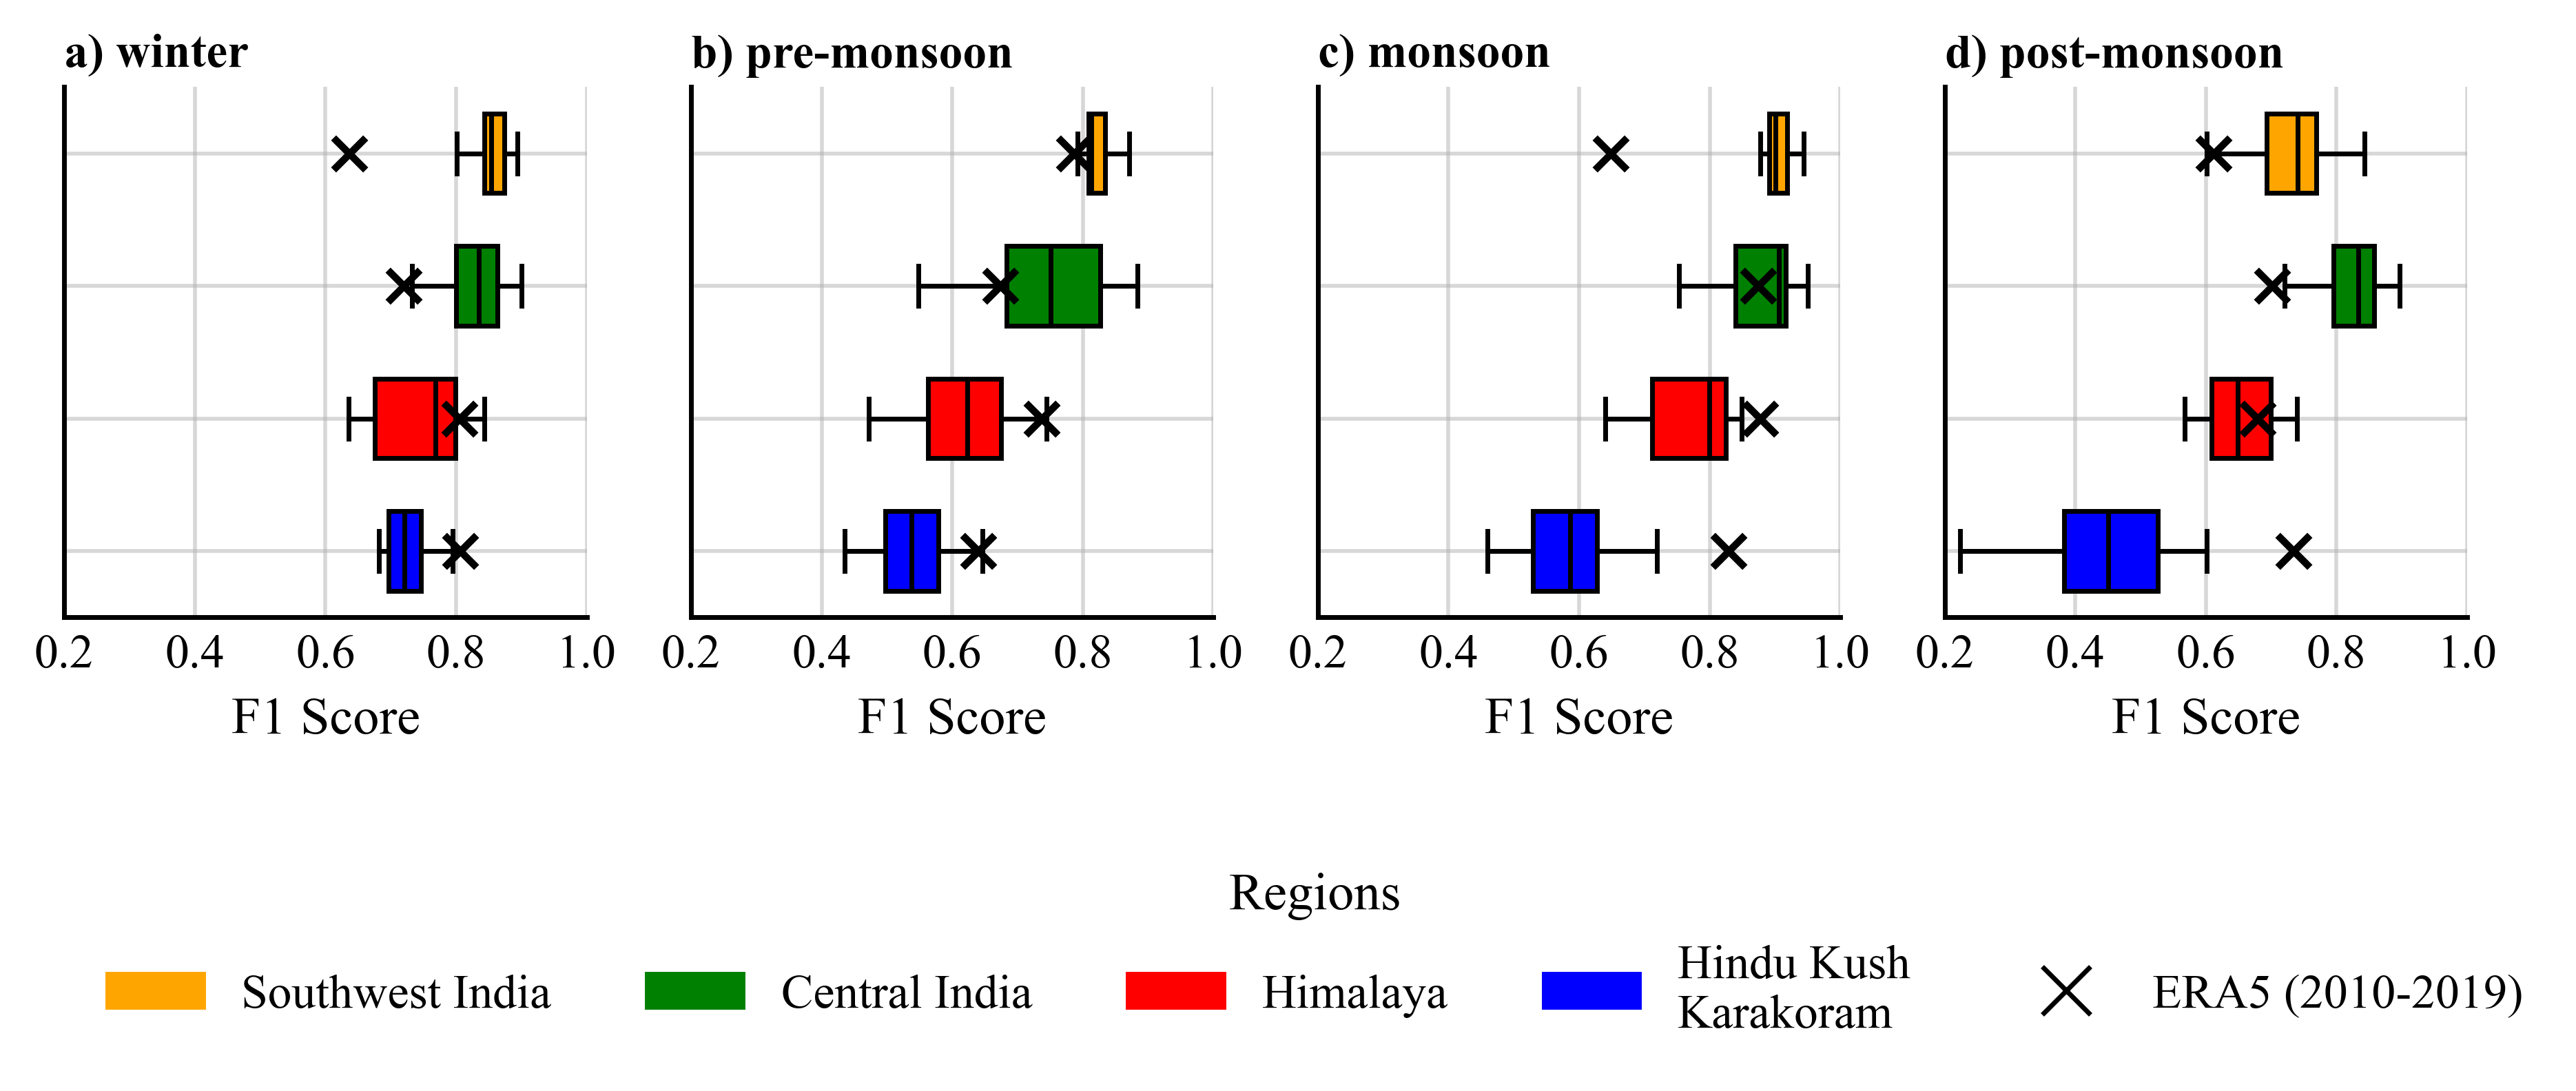
\includegraphics[width=0.9\textwidth]{Chapter3/figs/f1_scores.png}
\caption{Distribution of F1 scores computed for each season and CMIP6 model over the four representative regions during the historical period 1961--2015. The black crosses show the corresponding scores obtained over the held-out ERA5 period 2010--2019. Comparing CMIP6 with the ERA5 reference helps distinguish limitations of the classifier from differences in the seasonal cycle represented by the climate models.}
\label{fig:f1_scores}
\end{figure}

The seasonal cycle is represented consistently across the CMIP6 ensemble in Central and Southwest India. Performance is particularly strong for the monsoon, with average F1 scores of $0.86 \pm 0.09$ in Central India and $0.91 \pm 0.02$ in Southwest India. The monthly distribution of classified days confirms that the models reproduce both the overall shape and timing of the monsoon season, with only a small delay in its onset and close agreement in its withdrawal (Figure~\ref{fig:seasonal_shapes}c,d). Performance is slightly lower during the pre- and post-monsoon periods, whose transitional character makes their boundaries less clearly distinguishable.

\begin{figure}[H]
    \centering
    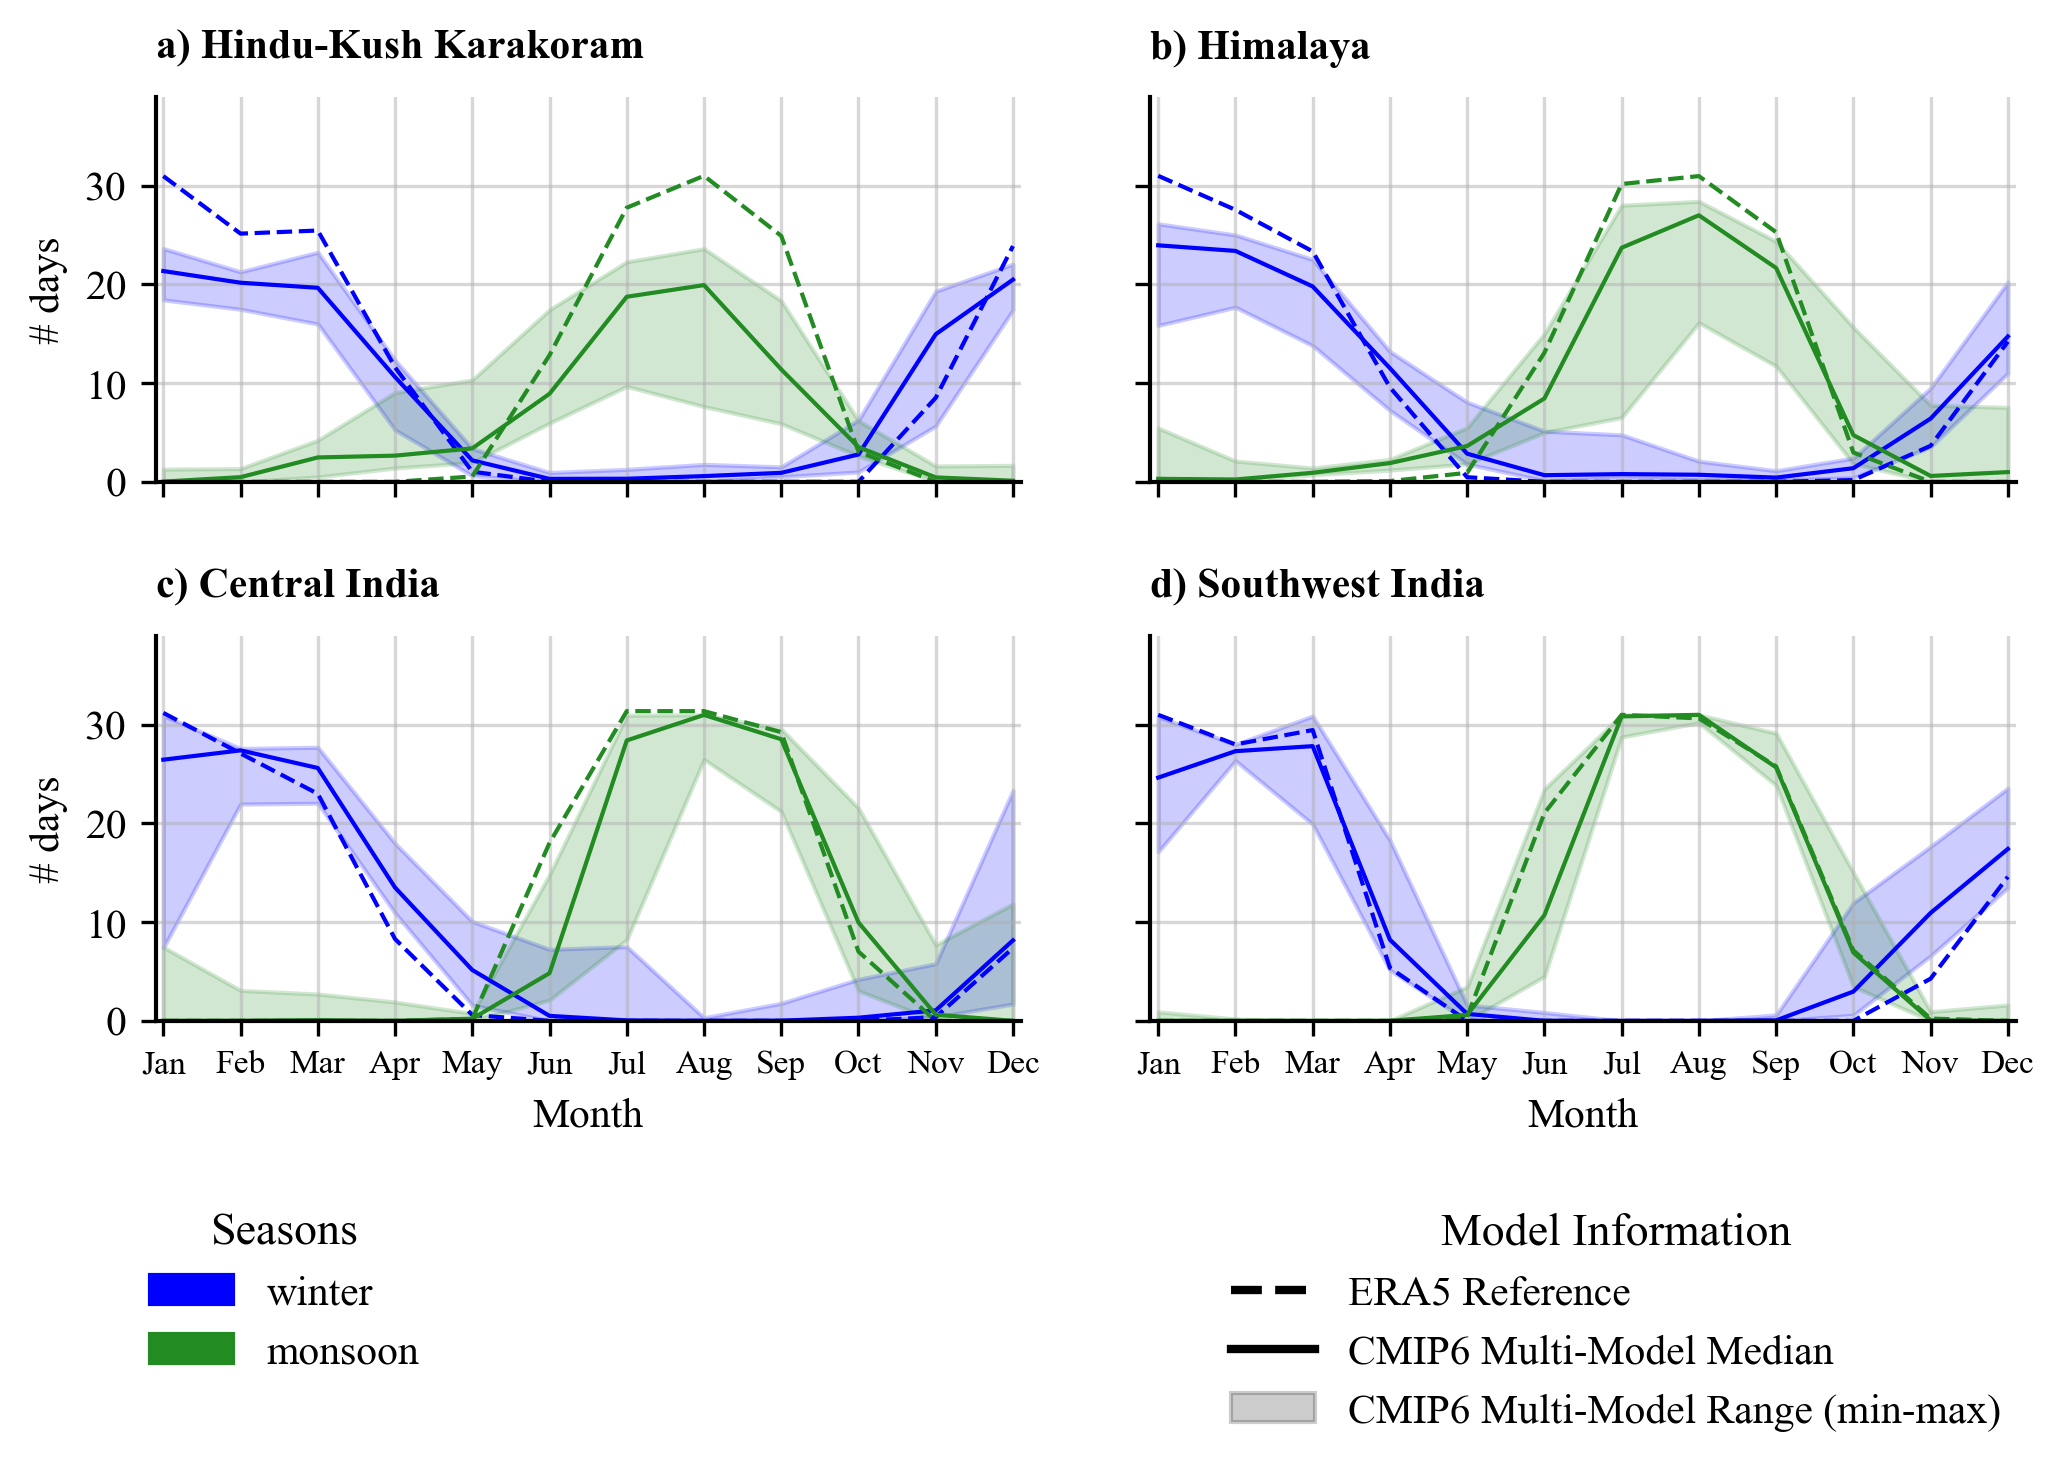
\includegraphics[width=0.9\textwidth]{Chapter3/figs/seasonal_shapes.png}
    \caption{Monthly distribution of days classified as winter and monsoon during the historical period over (a) Hindu Kush--Karakoram, (b) Himalaya, (c) Central India, and (d) Southwest India. Solid lines show the CMIP6 multi-model mean, shaded areas represent the inter-model range, and dashed lines show the seasonal classification derived from ERA5.}
    \label{fig:seasonal_shapes}
\end{figure}

The transfer is less successful in the mountain regions. Over the Hindu Kush--Karakoram, F1 scores are lower for the monsoon and transition seasons, with values ranging from $0.44$ for the post-monsoon to $0.56$ for the monsoon. The models reproduce the approximate timing of monsoon onset and withdrawal but classify fewer days as belonging to the monsoon during July and August (Figure~\ref{fig:seasonal_shapes}a). Because the corresponding ERA5 scores are generally higher, these differences appear to reflect primarily the difficulty of CMIP6 models in representing the regional seasonal cycle. The comparatively low ERA5 score during the pre-monsoon nevertheless indicates that this transition is also intrinsically more difficult to separate.

The Himalaya region shows intermediate performance, with F1 scores generally ranging between $0.6$ and $0.8$. The larger spread across models indicates that the representation of seasonality is less consistent than in Central and Southwest India. In both mountain regions, complex topography and the interaction between the summer monsoon and winter circulation make the seasonal cycle more difficult to reproduce. These results are consistent with the known ability of CMIP6 models to represent the main characteristics of the Indian monsoon \citep{khadka_evaluation_2022}, as well as with their limitations over the Himalayan region \citep{gusain_added_2020,lalande_climate_2021}.

The analysis shows that the seasonal definitions learned from reanalysis data can be transferred successfully to climate models where the underlying climatic regimes are represented with sufficient accuracy. At the same time, it demonstrates that the information obtained from the classification cannot be interpreted independently of model skill. For this reason, only models achieving an F1 score greater than $0.7$ for a given grid point and season were retained in the Significant Multi-Model Ensemble used for the analysis of future changes. This selection ensures that projected changes are evaluated only where the historical seasonal cycle is represented with adequate reliability.


\subsection{Projected Changes in Seasonality}

Having established where the ERA5-derived seasonal definitions can be transferred reliably to climate models, we applied the framework to future CMIP6 projections to investigate how the annual cycle may evolve during the twenty-first century. The analysis focuses primarily on the monsoon and winter seasons, which exhibit the clearest climatic signals and the greatest societal relevance. 

For each grid point and season, we retained only the models with an historical F1 score greater than $0.7$. This subset, referred to as the Significant Multi-Model Ensemble (SMME), accounts for the regional differences in the ability of CMIP6 models to reproduce the observed seasonal cycle. As summarized in Table~\ref{tab:smme_median_percentage}, nearly all models satisfy this criterion in Central and Southwest India, whereas considerably fewer models are retained over the Himalaya and Hindu Kush--Karakoram. Projected changes over the mountain regions should therefore be interpreted with greater caution.

\begin{table}[H]
\centering
\caption{Median number of models included in the Significant Multi-Model Ensemble for each season and region. Percentages refer to the complete ensemble of 13 models.}
\begin{tabular}{lcccc}
\hline
\textbf{Region} & \textbf{Winter} & \textbf{Pre-monsoon} & \textbf{Monsoon} & \textbf{Post-monsoon} \\
\hline
Hindu Kush--Karakoram & 8 (62\%) & 2 (15\%) & 6 (46\%) & 1 (8\%) \\
Himalaya              & 9 (69\%) & 6 (46\%) & 10 (77\%) & 7 (54\%) \\
Central India         & 12 (92\%) & 10 (77\%) & 12 (92\%) & 11 (85\%) \\
Southwest India       & 13 (100\%) & 12 (92\%) & 13 (100\%) & 12 (92\%) \\
\hline
\end{tabular}
\label{tab:smme_median_percentage}
\end{table}

Future changes were examined from three complementary perspectives. Figure~\ref{fig:spatial_trends} shows the spatial distribution of long-term trends in seasonal duration, while Figure~\ref{fig:seasonal_increment} describes their evolution within the four representative regions. The monthly analyses in Figures~\ref{fig:monthly_increment_monsoon} and \ref{fig:monthly_increment_winter} show which parts of each season contribute to the projected changes, allowing shifts in onset and withdrawal to be distinguished from uniform changes in duration.

\begin{figure}[H]
    \centering
    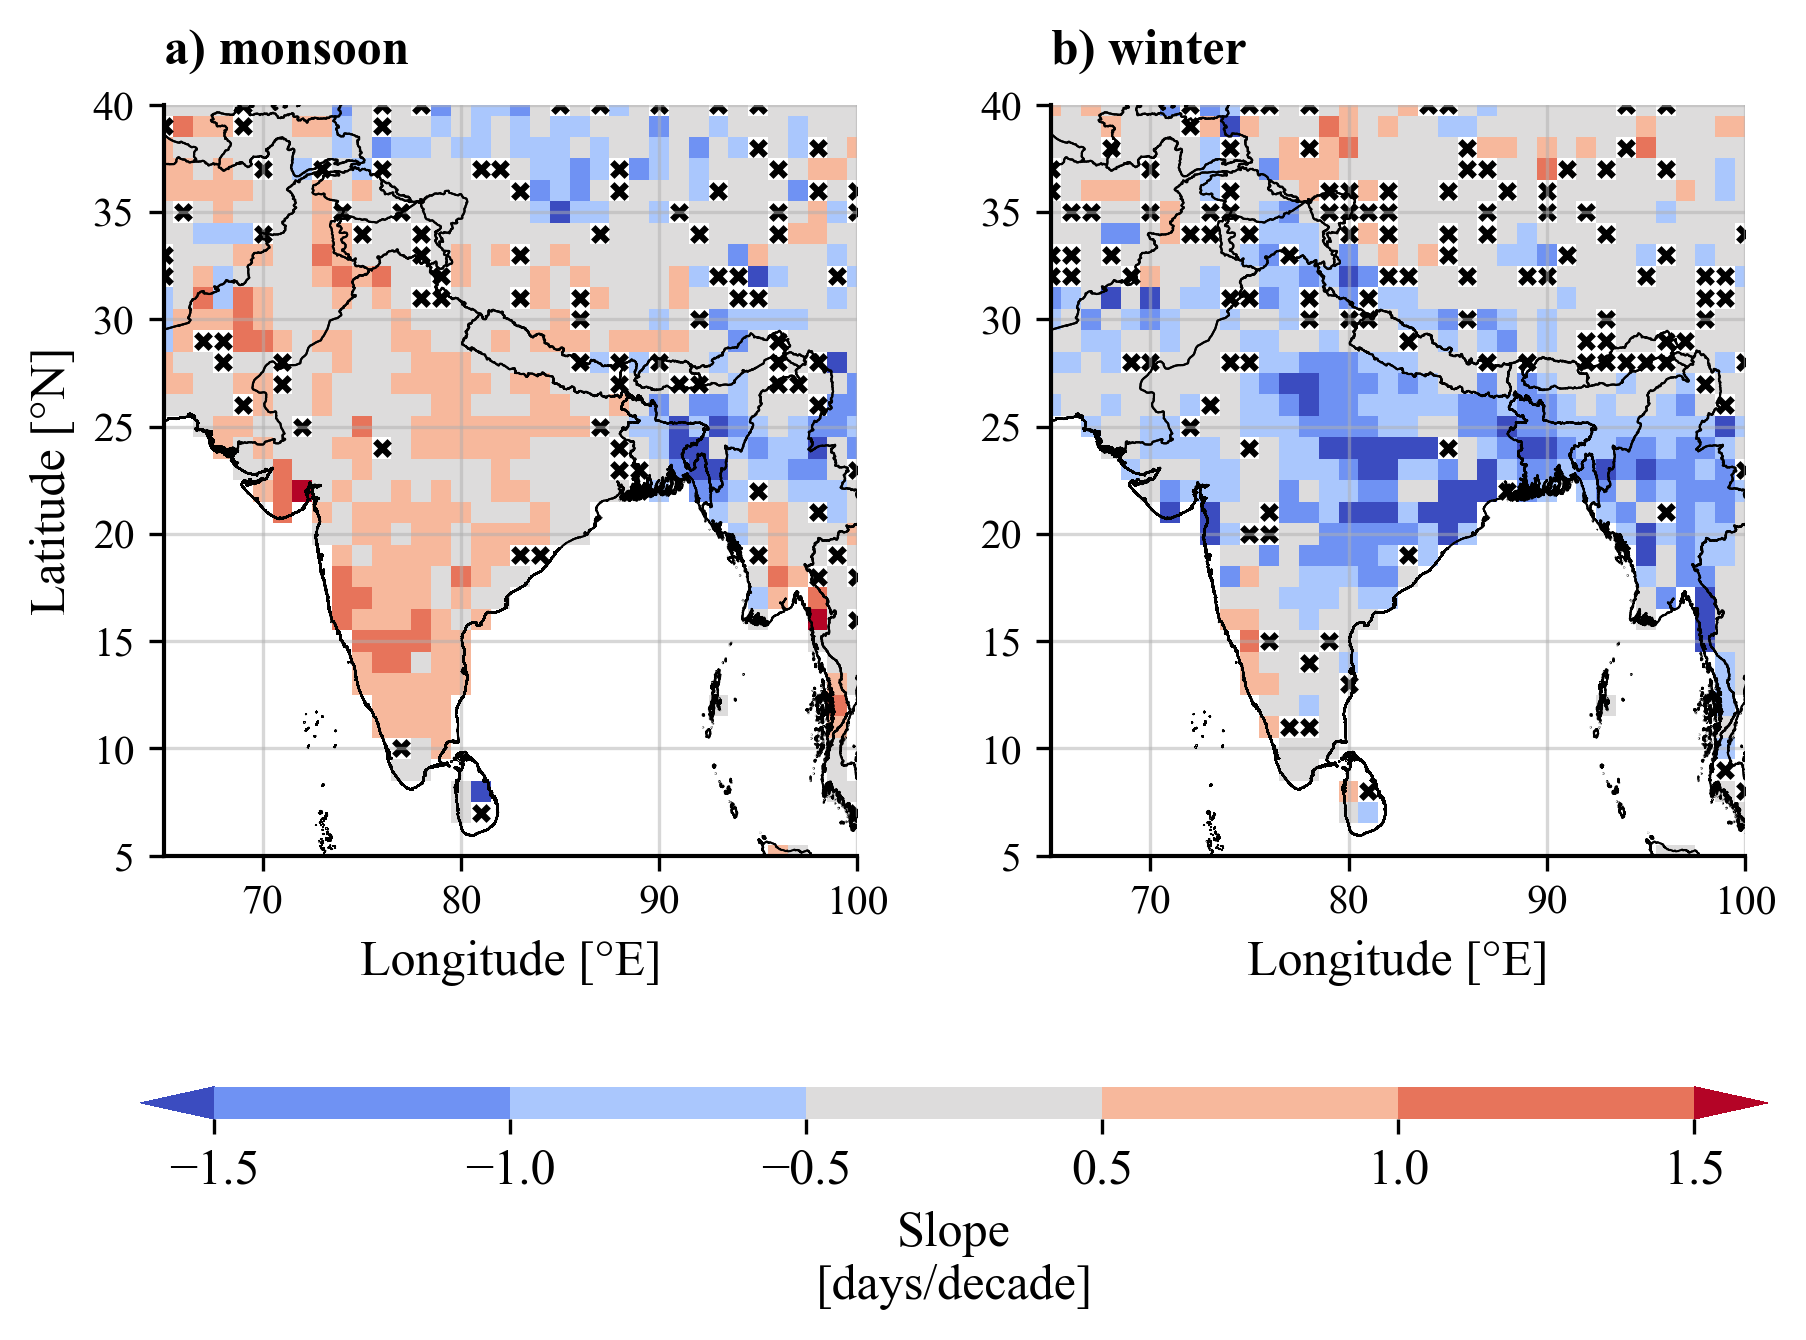
\includegraphics[width=0.7\textwidth]{Chapter3/figs/spatial_trends.png}
    \caption{Spatial distribution of linear trends in the number of days classified as monsoon (a) and winter (b) over the Indian subcontinent during 2020--2100. Trends are expressed in days per decade and computed from the SMME mean. Only trends significant at the 95\% confidence level according to the Mann--Kendall test are shown \citep{gilbert_statistical_1987}. Black crosses identify grid points without statistically significant trends.}
    \label{fig:spatial_trends}
\end{figure}

\begin{figure}[H]
    \centering
    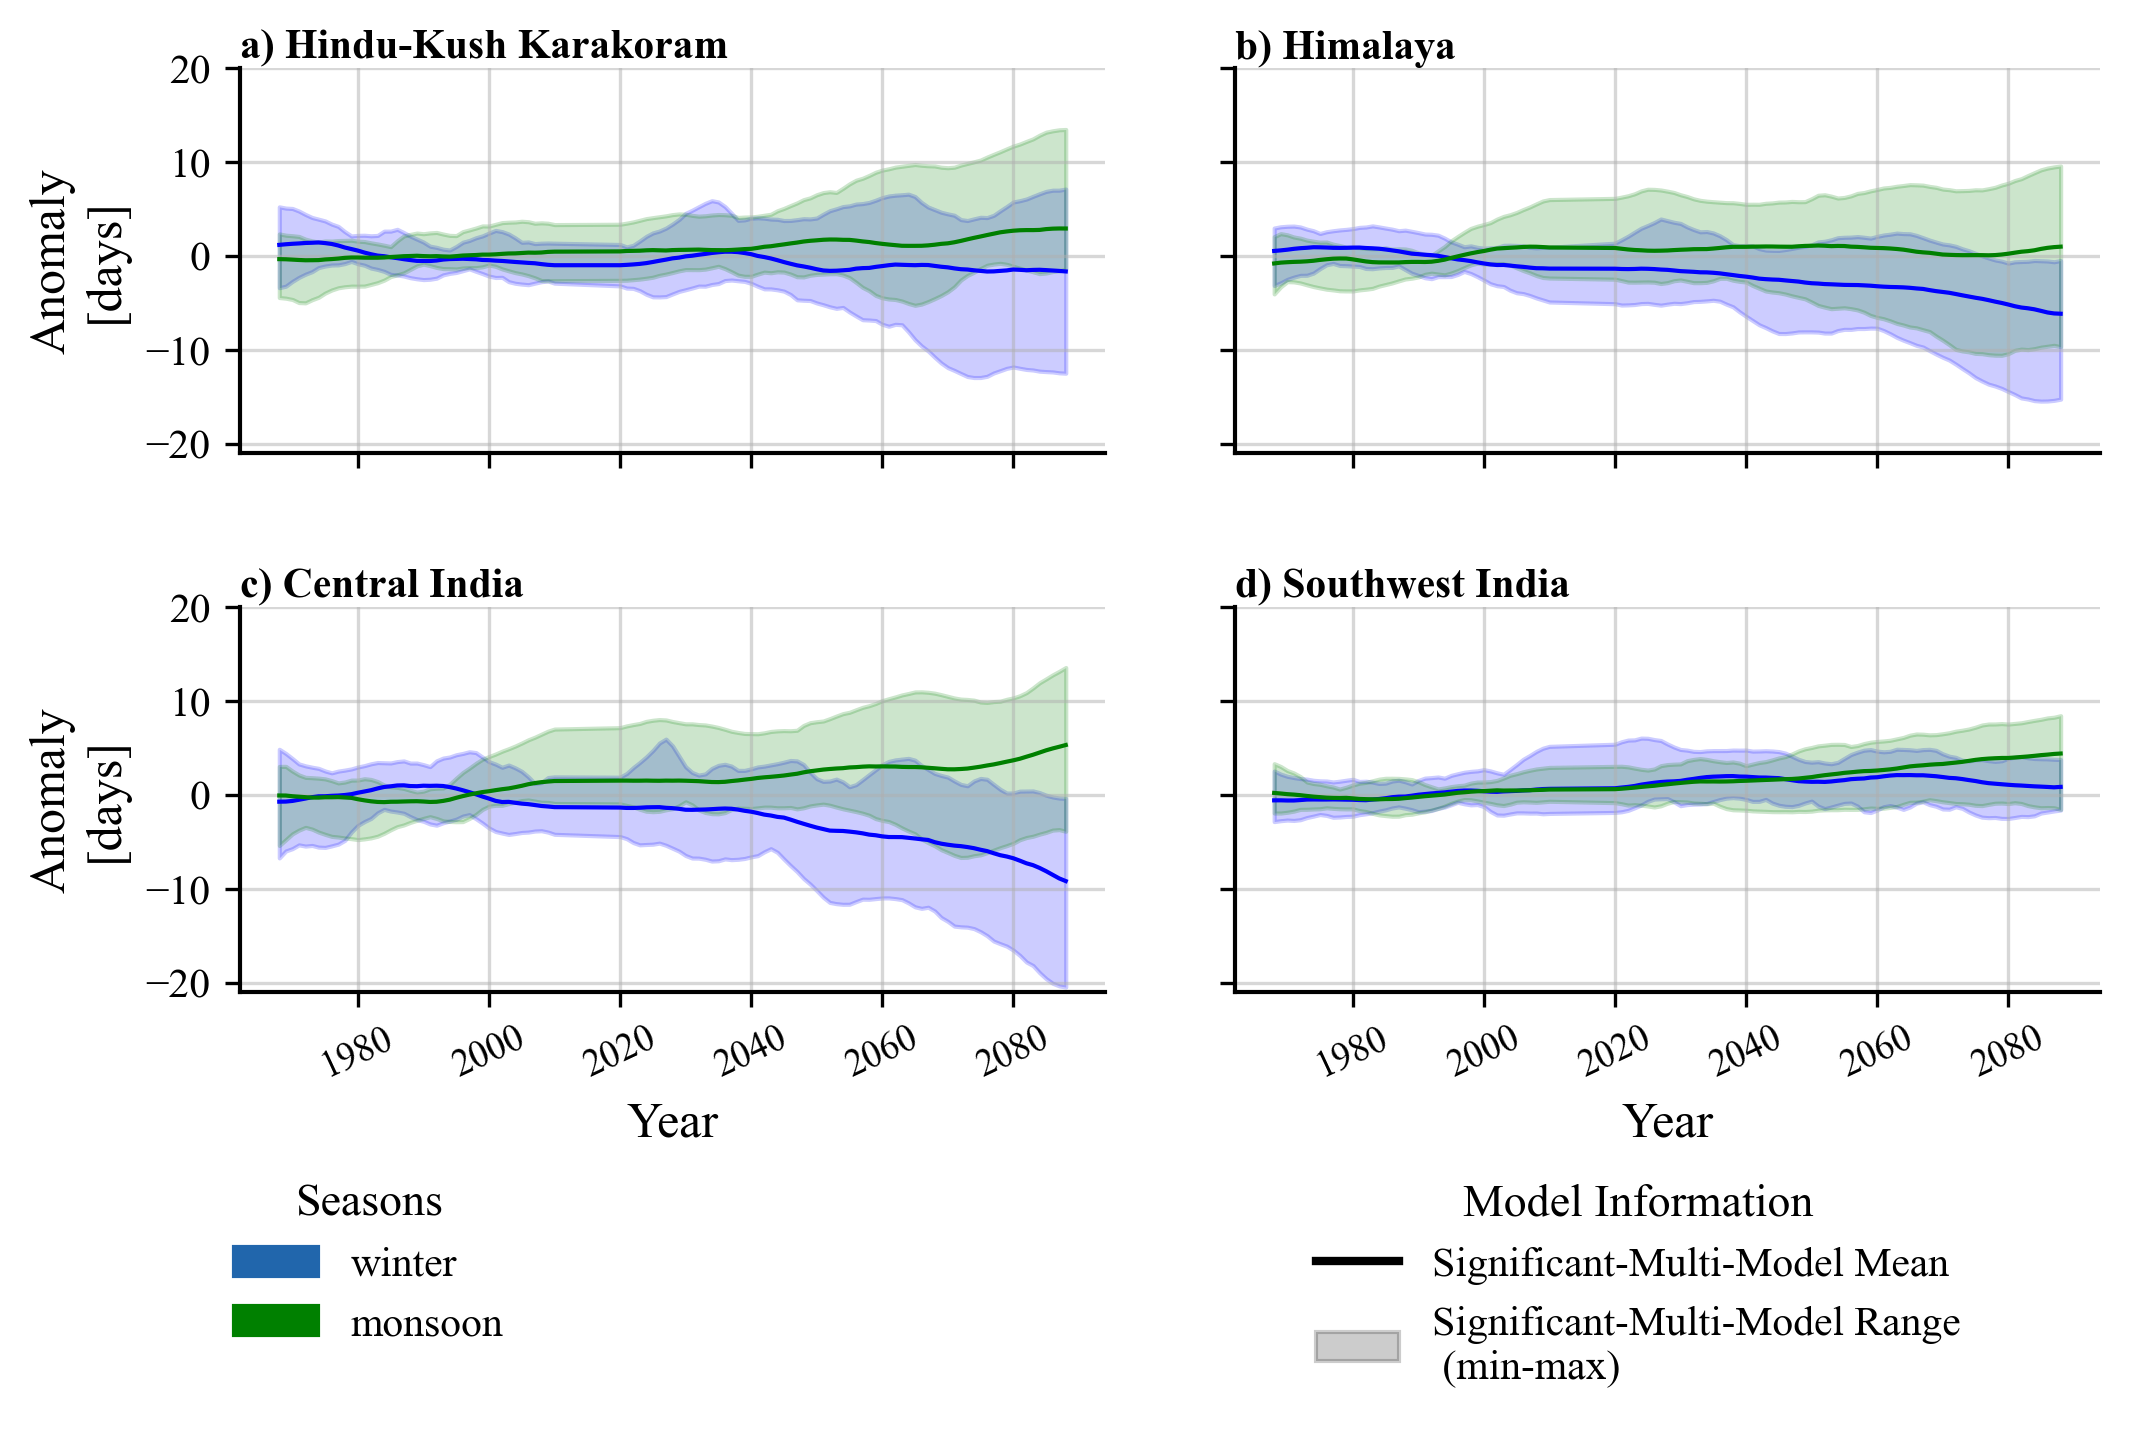
\includegraphics[width=0.9\textwidth]{Chapter3/figs/seasonal_increment.png}
    \caption{Projected anomalies in winter and monsoon duration over the four representative regions. Anomalies are computed relative to the historical mean seasonal length for 1970--2020 and smoothed using a 15-year centred rolling average. Solid lines represent the SMME mean and shaded areas show the inter-model range.}
    \label{fig:seasonal_increment}
\end{figure}

Most of the Indian subcontinent shows a significant lengthening of the monsoon season, particularly across Central, Western, and Southern India, where trends exceed $+0.5$ days per decade in several areas (Figure~\ref{fig:spatial_trends}a). Signals are weaker and less spatially coherent in northern and northeastern regions.

Central and Southwest India exhibit the clearest changes, with the monsoon projected to lengthen by approximately five days by the end of the century (Figure~\ref{fig:seasonal_increment}c,d). This extension is asymmetric: monsoon onset changes only slightly, while withdrawal occurs progressively later (Figure~\ref{fig:monthly_increment_monsoon}c,d). The result therefore indicates a persistence of monsoon-like conditions into the later part of the annual cycle rather than a uniform expansion at both seasonal boundaries.

The Himalayan region shows little change in total monsoon duration, but its internal timing shifts by approximately two days from the early to the late part of the season (Figure~\ref{fig:monthly_increment_monsoon}b). No consistent trend emerges over the Hindu Kush--Karakoram, where models produce a combination of weak positive and negative changes. The low historical skill and limited number of models retained in the SMME further reduce confidence in projections for this region.

These results are broadly consistent with CMIP6 studies projecting an increase in Indian monsoon precipitation, wet days, and heavy precipitation under global warming \citep{wang_understanding_2020,norgate_present_2024,dhara_post-ar6_2025}. Previous analyses based on precipitation thresholds have also identified a delayed withdrawal of the Indian Summer Monsoon \citep{ha_future_2020,wang_rainy_2002}. The present framework reaches a similar conclusion using a multivariate classification of the regional atmospheric state.

However, the direction of projected changes depends on how the monsoon is defined. Using a large-scale indicator based on the upper-tropospheric temperature gradient, \citet{cheng_shorter_2025} found a shortening of the monsoon under a high-emission scenario, characterized by delayed onset and earlier withdrawal. This apparent contrast reflects the fact that the two approaches describe different components of the monsoon system. The large-scale temperature gradient represents the establishment and decay of monsoon circulation, whereas the classification used here identifies the persistence of local hydroclimatic conditions. This distinction is particularly relevant in Central India, where precipitation accounts for 49\% of the relative importance of the variables used to identify the monsoon class (Table~\ref{tab:feature_importance}). Under warming, precipitation and large-scale circulation need not evolve synchronously because increased atmospheric moisture can intensify rainfall even when circulation weakens \citep{ma_paradox_2014}. A direct comparison applying both definitions to the same simulations would nevertheless be required to determine the exact origin of the difference.

\begin{figure}[H]
    \centering
    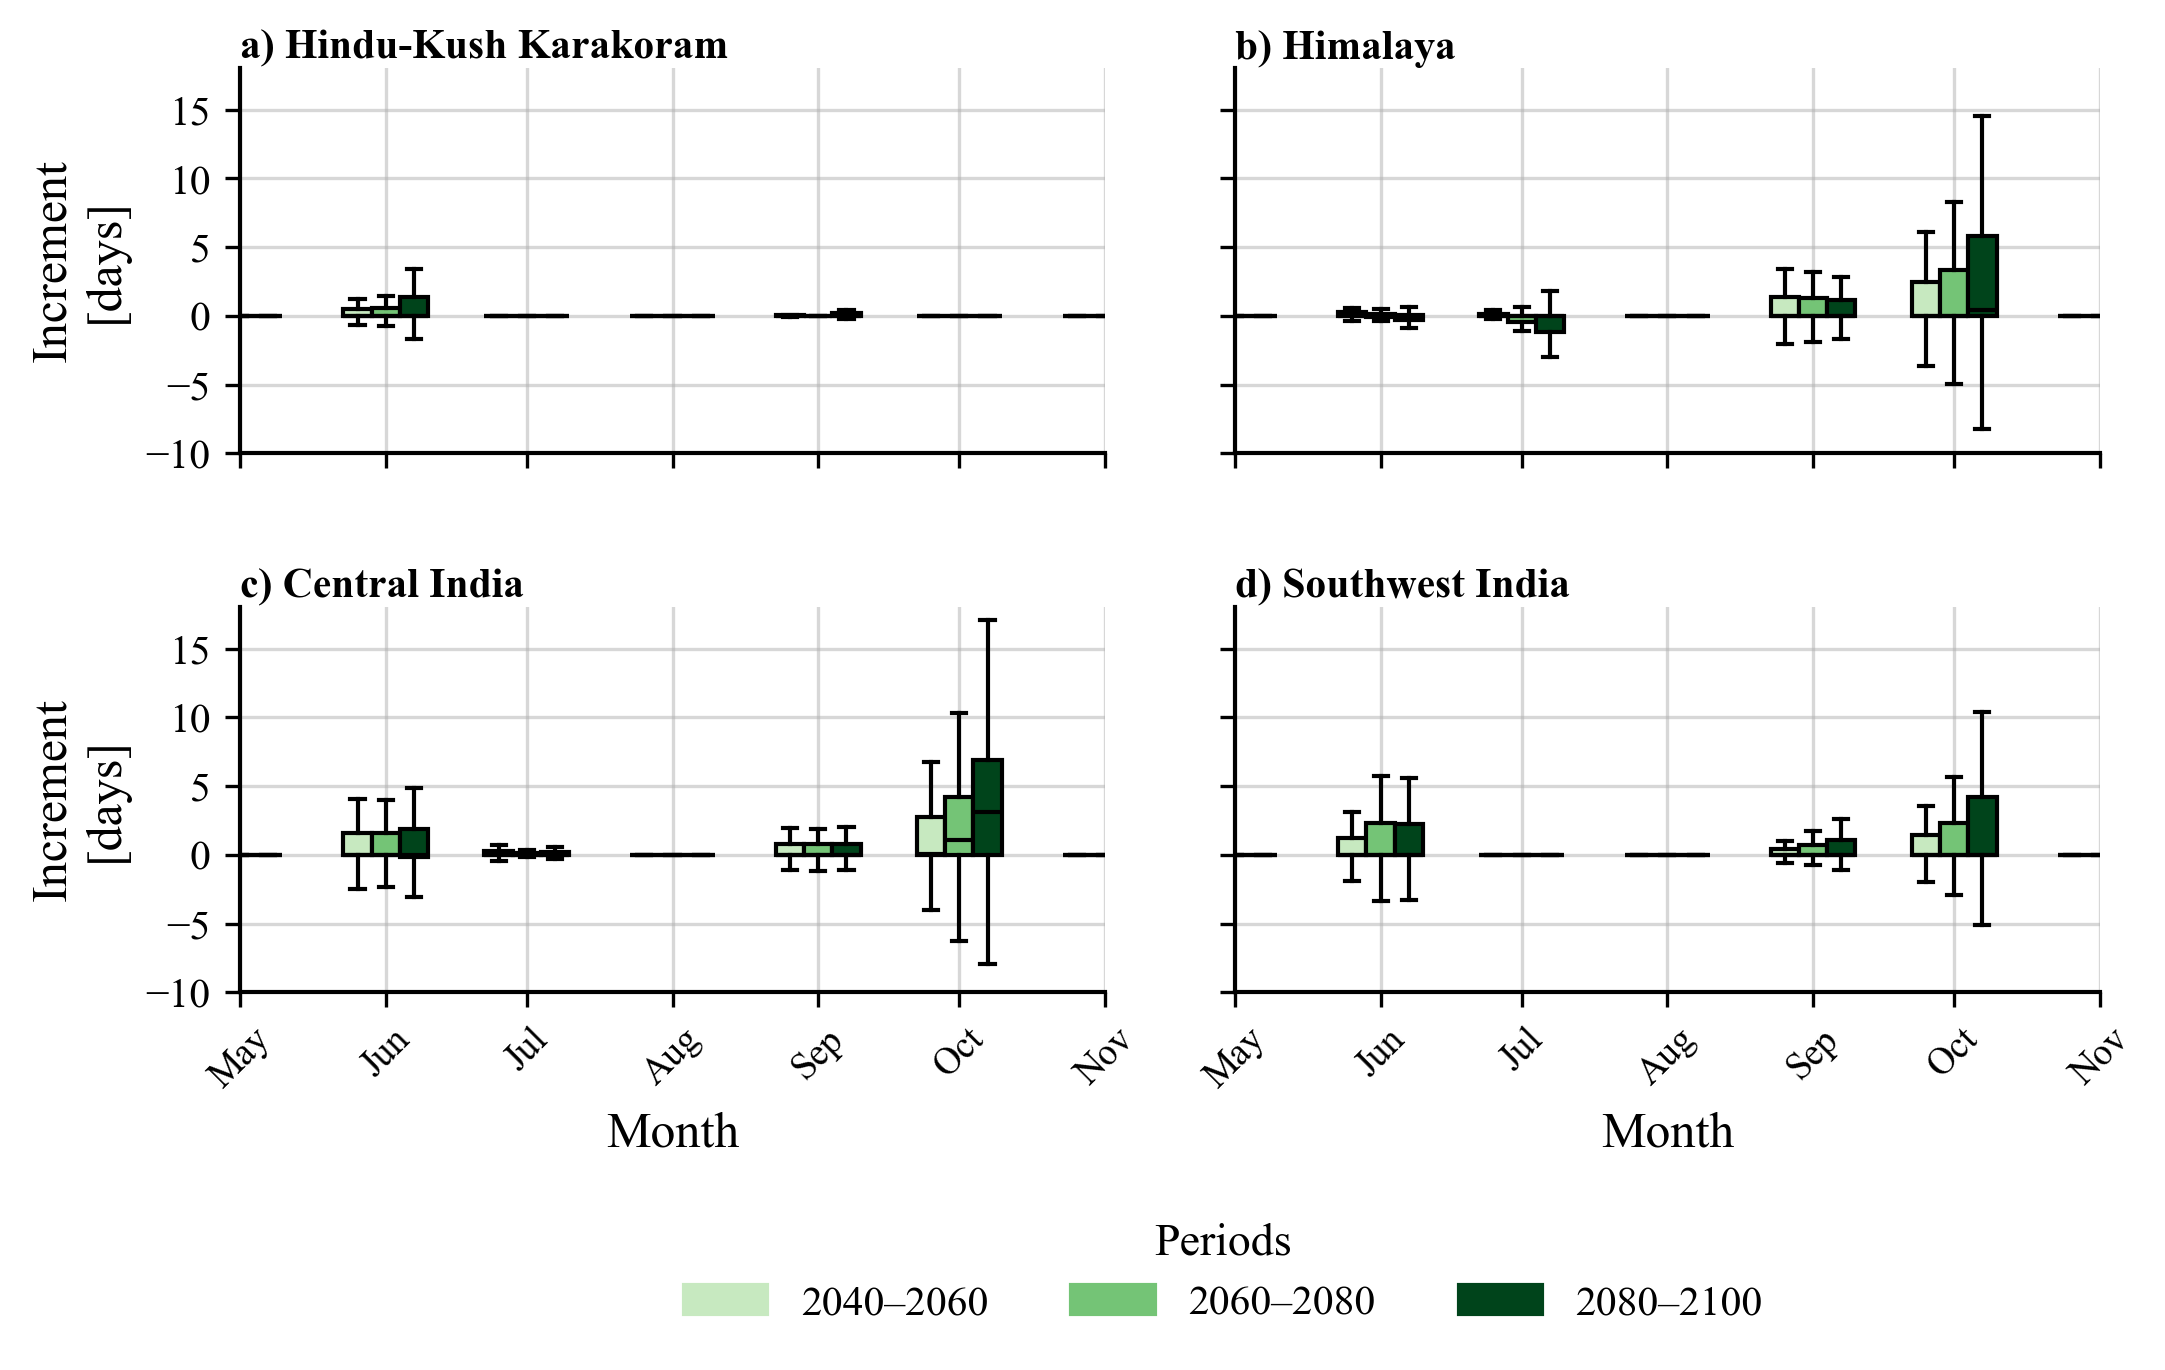
\includegraphics[width=0.9\textwidth]{Chapter3/figs/monthly_increment_monsoon.png}
    \caption{Projected monthly change in the number of days classified as monsoon during three future periods, relative to the 1970--2000 climatology. Each panel represents one of the four subregions, and the distributions combine grid points and models included in the SMME.}
    \label{fig:monthly_increment_monsoon}
\end{figure}

The winter season shows an opposite tendency. Its duration decreases across much of the subcontinent, particularly in Central and Southern India, where trends reach approximately $-1.5$ days per decade (Figure~\ref{fig:spatial_trends}b). Although negative trends also appear in the mountain regions, they are less spatially coherent and are frequently not statistically significant.

Central India experiences the largest change, with a projected loss of up to ten winter days by the end of the century (Figure~\ref{fig:seasonal_increment}c). The contraction becomes more pronounced after 2040 and is concentrated mainly in December and January. The Himalaya shows a similar but weaker signal, with a reduction of approximately five winter days by 2100 (Figure~\ref{fig:seasonal_increment}b). In contrast, neither Southwest India nor the Hindu Kush--Karakoram exhibits a coherent regional change. Over Southwest India, local trends have opposing signs, while projections over the Hindu Kush--Karakoram remain limited by low model agreement and historical skill.

The projected shortening should not be interpreted simply as the direct effect of increasing temperature. The preprocessing applied in this framework removes long-term changes in the mean and variance of the individual climate variables. The classification therefore responds to changes in their intra-annual distribution and relationships rather than to the mean warming trend itself. In Central India, for example, the winter class is defined primarily by precipitation and low-level zonal circulation rather than by temperature alone (Table~\ref{tab:feature_importance}). The loss of winter days consequently indicates that the multivariate conditions associated with winter become less frequent or less distinct from those of the surrounding seasons.

Temperature plays a larger role in identifying winter over the Himalaya and Hindu Kush--Karakoram, where it accounts for approximately 43\% and 44\% of relative feature importance, respectively. Nevertheless, the strong warming projected over these regions does not produce a coherent winter shortening over the Hindu Kush--Karakoram. This result further illustrates that changes in a single variable do not necessarily correspond to changes in the multivariate seasonal state captured by the classification.

\begin{figure}[H]
    \centering
    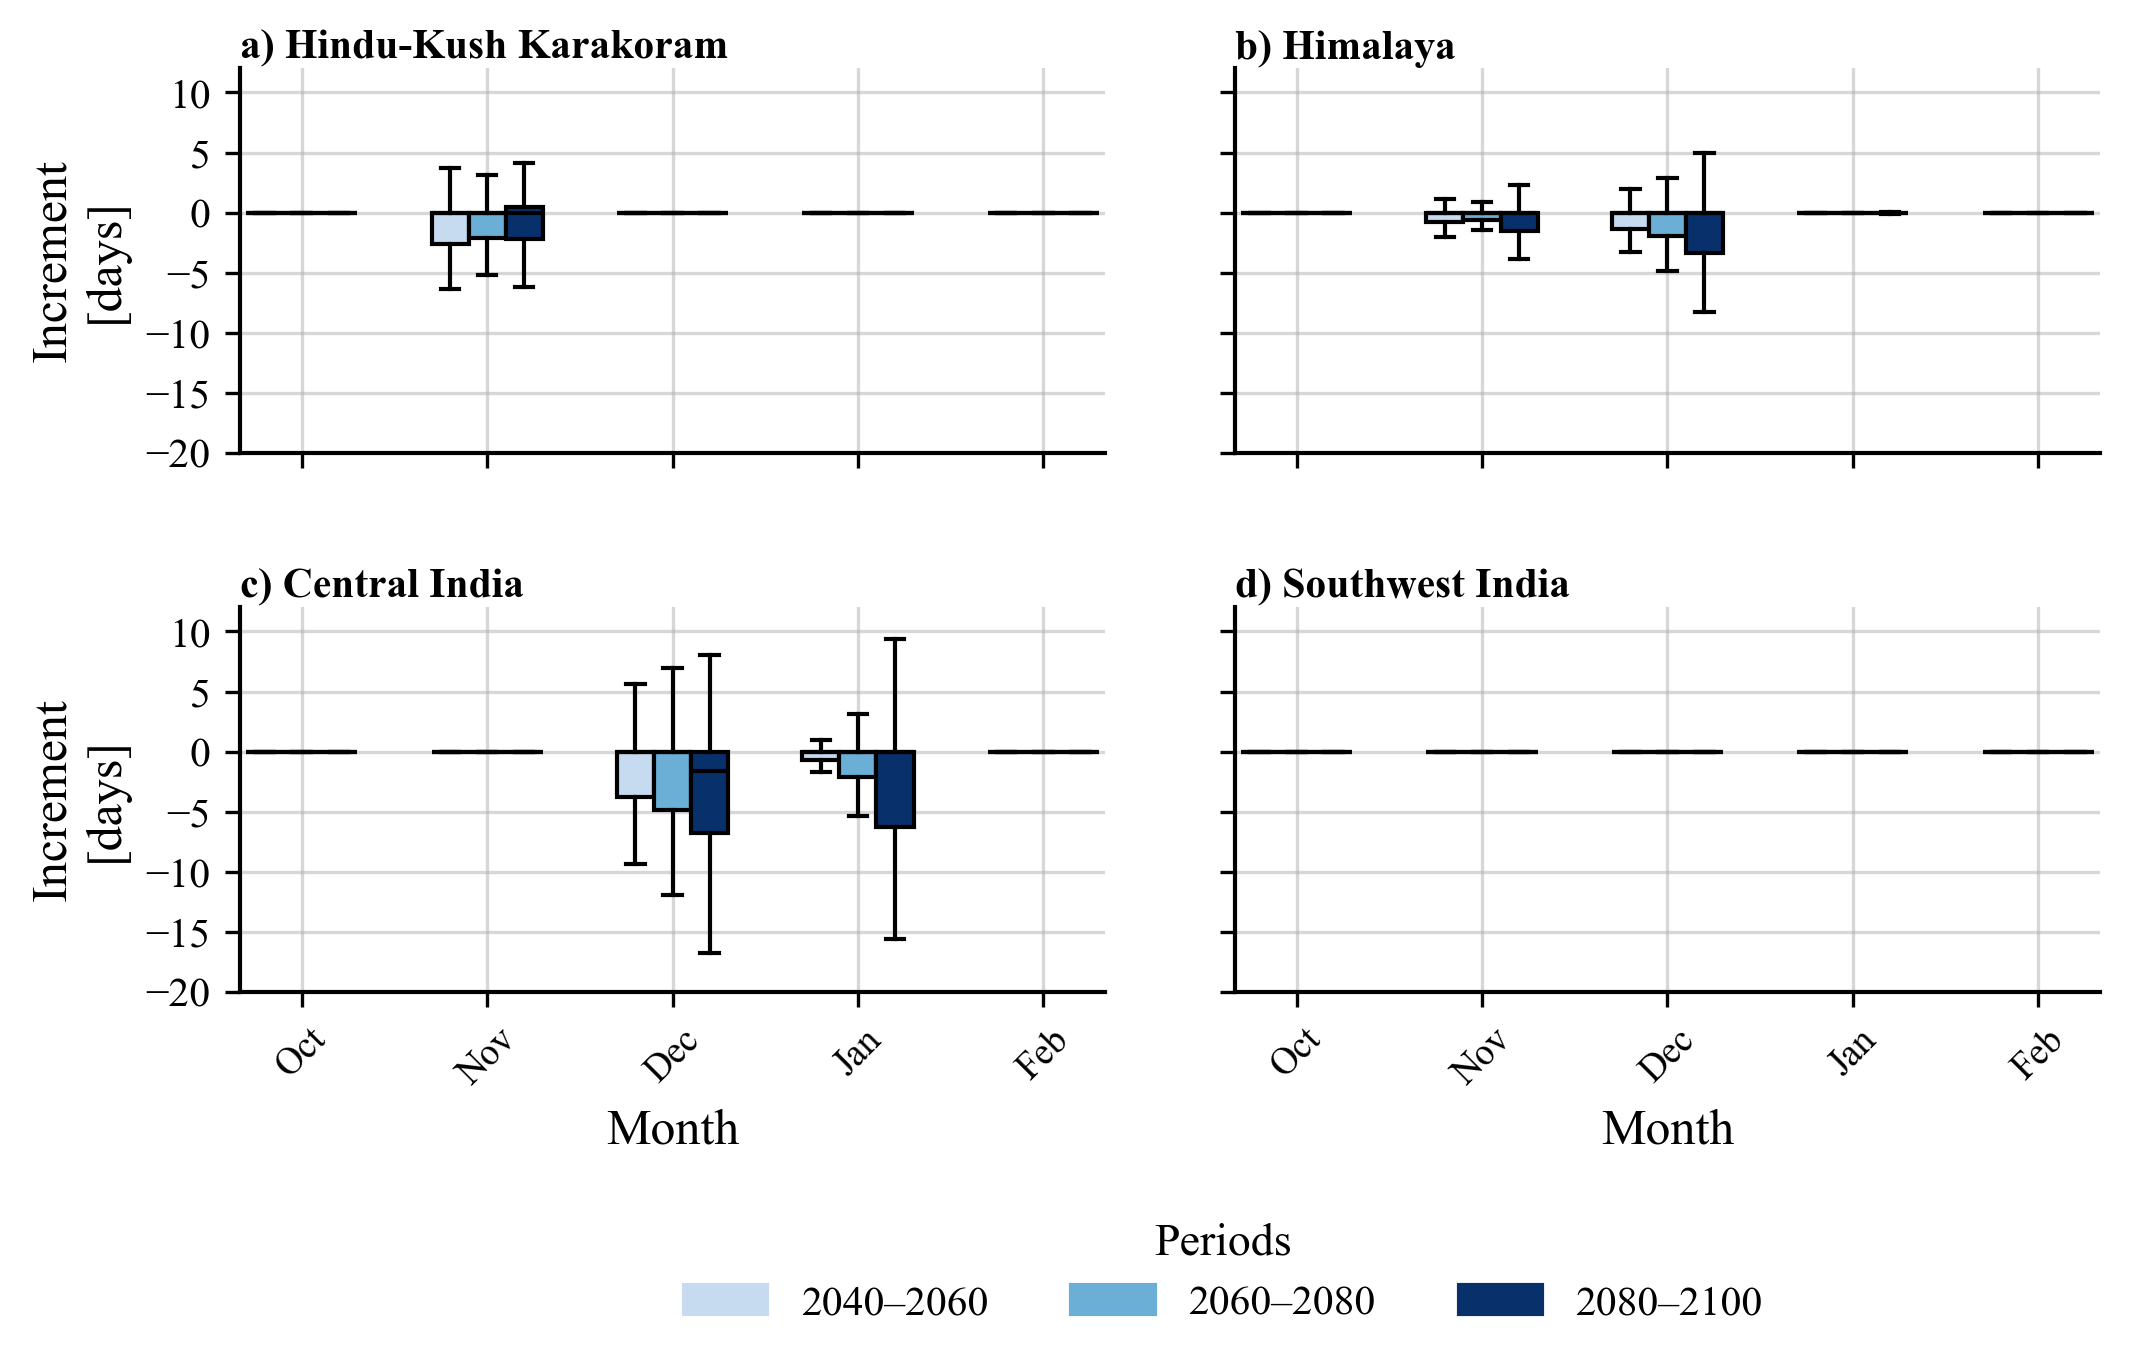
\includegraphics[width=0.9\textwidth]{Chapter3/figs/monthly_increment_winter.png}
    \caption{Projected monthly change in the number of days classified as winter during three future periods, relative to the 1970--2000 climatology. Each panel represents one of the four subregions, and the distributions combine grid points and models included in the SMME.}
    \label{fig:monthly_increment_winter}
\end{figure}

Overall, the projections indicate that seasonal changes are not uniform shifts of the annual cycle. The monsoon tends to persist later into the year, while the contraction of winter is concentrated in specific months and varies substantially across regions. 



\section{Discussion}

This chapter started from a simple question: how can information about meteorological seasons be inferred from climate data, given their heuristic nature? Seasons are familiar concepts, but climate datasets do not contain explicit labels indicating where one season ends and another begins. Their identification requires continuous and multivariate atmospheric conditions to be translated into discrete and interpretable categories.

The results show that this translation can be performed using a relatively simple Machine Learning framework. The seasonal partition learned from ERA5 broadly reproduces the annual cycle conventionally used to describe the Indian climate, including the monsoon, winter, and the two transition periods. Its consistency with the IMD monsoon patterns suggests that the clustering captures recognizable climatic structures rather than merely producing a mathematically convenient separation of the data. The analysis of the classifier also shows that these structures emerge from different combinations of temperature, precipitation, and circulation, depending on the season and region.

The resulting definitions should not be interpreted as replacements for the operational criteria adopted by the IMD. Operational definitions are designed to identify specific events and respond to established institutional needs. The framework developed here instead provides a multivariate description of the complete annual cycle. Its value lies in producing a consistent seasonal representation that can be applied beyond the dataset from which it was derived.

This transferability was tested by applying the ERA5-based definitions to CMIP6 simulations. The results show that the approach performs well where climate models reproduce the dominant seasonal regimes, particularly in Central and Southwest India. Its performance is less robust over the Himalaya and Hindu Kush--Karakoram, where complex topography and the interaction of different circulation systems remain challenging for global climate models. This indicates that the reliability of the information produced by the algorithm cannot be evaluated independently of the quality of the underlying climate data.

For this reason, model skill was incorporated directly into the analysis of future changes. The resulting projections indicate a lengthening of the monsoon over large parts of Central and Southern India, mainly because of delayed withdrawal, together with a shortening of winter concentrated in December and January. These changes do not represent simple shifts of fixed calendar boundaries. Instead, they describe changes in the persistence and timing of the multivariate atmospheric conditions associated with each seasonal regime.

At the same time, these results illustrate that climate data do not contain a single, universally valid definition of a season. For example, the monsoon lengthening identified here differs from the shortening found using a large-scale circulation indicator by \citet{cheng_shorter_2025}. The two approaches describe different components of the monsoon system: one identifies the persistence of regional hydroclimatic conditions, while the other describes changes in large-scale circulation. The information obtained from climate data therefore depends on the variables, scale, and definition adopted.

The data-driven character of the framework should consequently not be understood as the absence of assumptions. The number of seasons, the input variables, the temporal smoothing, and the normalization procedure are all part of the definition being constructed. Machine Learning avoids prescribing separate thresholds for individual variables, but it does not remove the scientific choices required to formulate the problem. These choices must remain transparent if the resulting indicators are to be interpreted correctly.

Within the Climate Services value chain, the framework performs an inference step: it transforms large volumes of climate data into indicators of seasonal timing and duration. These indicators are more accessible and comparable than the original multivariate datasets, but they are not yet decision-relevant knowledge. A delayed monsoon withdrawal, for example, acquires practical meaning only when connected to a specific context such as crop calendars, reservoir management, or flood risk.

The case study therefore demonstrates both the potential and the limits of AI in transforming climate data into information. The contribution of the algorithm does not lie simply in detecting patterns, but in producing a representation that can be validated physically, transferred across datasets, and evaluated according to the reliability of the underlying models. These conditions are essential for algorithmic outputs to become credible climate information and, through further contextualization, contribute to decision-relevant knowledge.
\chapter{Climate Knowledge in Large Language Models}

% **************************** Define Graphics Path **************************
\ifpdf
    \graphicspath{{Chapter4/Figs/}{Chapter4/Figs/PDF/}{Chapter4/Figs/}}
\else
    \graphicspath{{Chapter4/Figs/Vector/}{Chapter4/Figs/}}
\fi

\noindent\textit{Parts of this chapter are based on the work \emph{``Climate Knowledge in Large Language Models''}, by Kuznetsov, I., \textbf{Grassi, J.}, Pantiukhin, D., Shapkin, B., Jung, T., and Koldunov, N. The manuscript has been published in Artificial Intelligence for the Earth Systems, a journal of the American Meteorological Society.}

\vspace{0.5em}
\begin{center}
    \rule{0.5\textwidth}{0.4pt}
\end{center}
\vspace{0.5em}

The previous chapters examined how Artificial Intelligence can operate directly on numerical climate data: first by supporting their production through AI-based forecasting models, and then by extracting meaningful information from them through diagnostic Machine Learning methods. This and the following chapters moves to a different stage of the Climate Services value chain, where climate information must be organized, interpreted, and made accessible to users.

Large Language Models offer new possibilities at this stage. Their ability to interact through natural language may facilitate access to climate information for users with different levels of technical expertise. However, the fluency of their answers does not guarantee that the information they provide is accurate, traceable, or scientifically reliable. LLMs may generate responses using knowledge encoded in their parameters, retrieve information from external sources, or combine both mechanisms. Understanding the contribution and limitations of each component is therefore essential before these systems can be reliably integrated into Climate Services.

In this chapter, the focus is placed on the \emph{parametric knowledge} of LLMs: the information encoded in their parameters during training and available without access to external documents, datasets, or computational tools. This use of the term knowledge should be distinguished from the broader meaning adopted in the DIKW framework. While the latter refers to information interpreted and contextualized for a specific purpose, parametric knowledge describes what a language model can reproduce from its internal representation alone.

The central question addressed here is therefore: how accurately do LLMs represent quantitative climate information, and how does their reliability vary across locations and environmental conditions? To investigate this question, the chapter evaluates the ability of different LLMs to estimate historical temperature climatologies and observed warming across the globe. Their answers are compared with reference reanalysis data to assess geographical patterns, systematic biases, and the influence of the contextual information included in the prompts.

By establishing what LLMs can and cannot reliably provide in a closed-book setting, this chapter defines a baseline for their use in Climate Services. It also motivates the augmentation strategies examined in the following chapter, where language models are connected to external scientific literature, climate datasets, and analytical tools.

\section{Large Language Models as Interfaces to Climate Knowledge}

Climate Services do not consist solely of producing and distributing climate data. Their broader purpose is to mediate between scientific evidence and the users who need that evidence to understand risks, evaluate possible responses, and support decisions. This mediation requires the selection, interpretation, contextualization, and communication of information according to specific questions and user needs. Consequently, increasing the availability or resolution of climate data does not necessarily make climate information more accessible or usable \citep{findlater_climate_2021,doblas-reyes_linking_2021}.

Traditionally, this mediation has been provided through scientific reports, data portals, decision-support tools, and direct interaction with climate experts. Although these mechanisms remain essential, they often require users to identify appropriate sources, understand technical terminology, and navigate heterogeneous formats. Large Language Models introduce a different mode of interaction. By allowing users to formulate questions in natural language, they can potentially lower some of these technical barriers and provide a common interface to scientific documents, climate datasets, and model outputs.

LLMs act as an intermediate layer between available information and the user: they select, combine, reformulate, and present content in response to a question. This gives them the potential to support the transformation of climate information into more accessible and contextualized knowledge. At the same time, it introduces uncertainty about the origin and reliability of the generated answers. Understanding how these systems construct their responses is therefore a prerequisite for evaluating their possible contribution to Climate Services.


\subsection{From Climate Information to Climate Knowledge}

Within the DIKW framework adopted in this dissertation, information becomes knowledge when it is interpreted and connected to a specific context, question, or objective. Climate information may describe, for example, the historical temperature of a region, the projected change in precipitation, or the expected frequency of an extreme event. On its own, however, this information does not necessarily explain why the change is relevant, which activities may be affected, or how it should be interpreted by a particular user.

The transition from information to knowledge therefore involves more than the extraction of indicators from data. It requires the combination of different sources, the identification of relevant relationships, and the communication of results in a form that can be understood and interrogated. This process is particularly challenging in climate applications because the available evidence is distributed across scientific literature, observational records, reanalysis products, climate model simulations, and sector-specific studies. These sources differ in their spatial and temporal scales, assumptions, uncertainties, and intended audiences.

LLMs may support this transition in several ways. They can summarize scientific material, explain technical concepts, compare information from different sources, and adapt the form of an answer to the question posed by the user. Unlike static reports or conventional data portals, a conversational interface also enables an iterative interaction in which users can refine their questions, request clarification, or explore different aspects of the same problem. Recent climate-oriented assistants have therefore investigated the use of LLMs as interfaces to scientific literature and other climate information sources \citep{vaghefi_chatclimate_2023,koldunov_local_2024}.

Nevertheless, an answer expressed in accessible and coherent language cannot automatically be considered knowledge. LLMs generate text by modelling statistical relationships between linguistic elements, rather than by independently verifying the scientific validity of each statement. Their answers may omit relevant qualifications, combine information referring to different periods or locations, or express uncertain content with unjustified confidence. They may also provide little indication of the evidence on which a statement is based.

The contribution of LLMs to knowledge creation therefore depends not only on their ability to generate relevant text, but also on the reliability, provenance, and uncertainty of the information included in their answers. This makes it necessary to distinguish between information already encoded within the language model and information obtained from external and verifiable sources.


\subsection{Parametric Knowledge and External Knowledge Sources}

The information that an LLM acquires during training is commonly referred to as its \emph{parametric knowledge}. Rather than being stored as an explicit collection of documents or database entries, this information is represented implicitly through the parameters of the model. As a result, an LLM may reproduce factual information, geographical associations, or general climatic relationships without consulting an external source.

Parametric knowledge should not, however, be interpreted as a structured or authoritative database. The model generally cannot identify the specific source from which a piece of information originated, determine whether it remains current, or guarantee that different elements of an answer refer to consistent datasets and reference periods. Its representation of a topic also reflects the frequency, geographical coverage, and quality of the material included in its training data. Widely documented locations and general global patterns may therefore be represented more accurately than less documented regions or geographically specific climate conditions.

For climate applications, this distinction is particularly important. An LLM may have learned general relationships such as the decrease of temperature with latitude or elevation, the seasonal contrast between hemispheres, or the approximate magnitude of global warming. These associations may allow it to produce plausible estimates for many locations. Plausibility, however, does not ensure the precision required for quantitative assessments, especially when local climate is influenced by topography, coastal effects, land cover, or regional circulation patterns.

Alternatively, an LLM can be connected to external knowledge sources. Retrieval-augmented systems provide the model with relevant passages from scientific documents, while tool-based systems may allow it to query climate databases, process numerical data, or interact with model outputs \citep{lewis_retrieval-augmented_2020}. These approaches can provide access to more precise and traceable information, but they do not completely replace the model's parametric knowledge. The LLM must still formulate queries, interpret retrieved material, combine different results, and communicate them to the user. Moreover, retrieval or tool use may not be available in every deployment or may not be activated for every question.

Evaluating parametric knowledge separately therefore provides an important baseline. It makes it possible to determine which aspects of climate information are already represented within an LLM, where systematic errors arise, and when external sources become necessary. It also helps distinguish improvements produced by retrieval or analytical tools from the capabilities of the underlying language model.

The remainder of this chapter isolates this closed-book component by asking LLMs quantitative and geographically specific questions without providing external climate data. Their answers are compared with authoritative reference information to evaluate whether the models reproduce broad climatological patterns, how their accuracy varies across space and environmental conditions, and whether they capture observed changes in climate. This evaluation establishes the baseline against which the augmented systems considered in the following chapter can be assessed.

\section{Evaluating Parametric Climate Knowledge}

The evaluation was designed as a closed-book benchmark of quantitative climate knowledge. Rather than asking the models to discuss general climate concepts, we posed questions for which an objectively verifiable numerical answer could be obtained from an authoritative climate dataset. This makes it possible to evaluate not only whether the answers are plausible, but also how closely they reproduce the magnitude and spatial structure of the reference climate information.

The benchmark focuses on near-surface air temperature. Temperature was selected because it is a widely understood climate variable, is available globally from reanalysis products, and exhibits well-defined spatial and seasonal patterns. At the same time, its local value depends on several geographical factors, including latitude, elevation, continentality, and proximity to the coast. It therefore provides a simple but informative test of whether LLMs encode both broad climatic regularities and geographically specific information.


\subsection{Evaluation Questions}

The evaluation was organized around four related questions. First, we asked whether LLMs can reproduce the geographical distribution of a present-day temperature climatology. This provides a test of whether their parameters encode broad climatic patterns, such as the contrast between tropical and high-latitude regions, as well as more localized variations.

Second, we investigated whether the accuracy of this knowledge depends on the geographical context provided to the model. Coordinates provide an unambiguous representation of location, but they may not be the format through which geographical information is most commonly represented in the textual material used to train an LLM. Country, region, and city names may instead act as linguistic anchors connecting the question to information encountered during training. The benchmark therefore compares prompts containing coordinates and geographical descriptors with prompts containing coordinates alone.

Third, we examined whether the ability to represent temperature climatology extends across the annual cycle. The main experiment focuses on July, while a second experiment evaluates all twelve calendar months for a subset of locations and models. This makes it possible to determine whether the conclusions obtained for a single month generalize to different seasons and to both hemispheres.

Finally, we assessed whether LLMs can represent not only the mean state of the climate but also its temporal evolution. For this purpose, the models were asked to estimate the change in mean July temperature between two historical periods. This last experiment distinguishes the recall of relatively static climatological information from the ability to represent geographically differentiated patterns of observed climate change.


\subsection{Reference Climate Information}

Reference values were obtained from the ERA5 reanalysis, which provides a physically consistent reconstruction of the atmosphere by combining observations with a numerical weather prediction model \citep{hersbach_era5_2020}. ERA5 was used as the reference because of its global coverage, temporal consistency, and widespread use in climate applications. The comparison should nevertheless be interpreted as agreement with the reanalysis rather than with direct observations at each individual location.

A regular grid with a resolution of \(1^{\circ}\) in latitude and longitude was generated between \(60^{\circ}\,\mathrm{S}\) and \(85^{\circ}\,\mathrm{N}\), covering the full range of longitudes. Antarctica and the northernmost Arctic regions were therefore excluded. After removing ocean cells, the evaluation domain contained 15,395 land grid points.

For each point, the primary reference variable was the mean July 2-m air temperature over the 1991--2020 climatological period. This period corresponds to a standard 30-year climate normal and provides the target for the main closed-book experiment. The resulting field contains a broad range of climatic conditions and allows the models to be evaluated consistently across different continents, latitudes, and elevations.

Each grid point was also associated with the nearest available country, administrative region, and city using the Nominatim reverse-geocoding service \citep{nominatim_nominatim_2026}. These descriptors were not used to determine the reference temperature. Their purpose was to test whether expressing the same location through familiar geographical names helps the models access information encoded in their parameters.

To evaluate the seasonal cycle, the reference dataset was extended to include the 1991--2020 mean 2-m air temperature for all twelve calendar months. Because of the computational cost of repeatedly querying the models, this experiment was conducted on a subset of 1,540 land points, obtained by retaining every tenth point from the original grid.

The magnitude of the model errors across the annual cycle was also compared with the natural interannual variability represented by ERA5. For each grid point and calendar month, yearly temperature anomalies were calculated relative to the corresponding 1991--2020 monthly mean. The root-mean-square of these anomalies provides an observational reference for the typical year-to-year variation in monthly temperature. It is used only as a scale for interpreting the LLM errors and not as an evaluation metric for the models themselves.

Finally, the climate-change experiment considered the difference in mean July temperature between the periods 1950--1974 and 2000--2024:

\begin{equation}
    \Delta T_i =
    \overline{T}_{i,\,2000\text{--}2024}
    -
    \overline{T}_{i,\,1950\text{--}1974},
\end{equation}

where \(i\) identifies a land grid point. The same difference was calculated from ERA5 and used as the reference against which the estimates produced by the LLMs were evaluated.


\subsection{Language Models and Prompting Strategies}

The benchmark included both proprietary and open-weight language models, covering different model families, parameter counts, and levels of domain specialization. The evaluated models included the GPT-5 family, GPT-OSS 120B and 20B, Mistral-small-3.1 24B, Gemma 27B and 12B, Gemini-2.5-flash-lite, Llama3.1 8B, Mistral-nemo 12B, Llama2 70B, and the domain-adapted eci-io-climategpt 70B. Considering the different sampling configurations, the main experiment comprised 17 model configurations.

Open-weight models were run locally through Ollama. To support reproducibility, the specific model images, parameter counts, and quantization settings are reported in Table~\ref{tab:model_configurations}. Proprietary models were accessed through their respective providers. Since their internal weights and quantization schemes are not publicly available, their configurations are identified through the model names and versions exposed by the providers.

All models were evaluated in a closed-book setting. They were not given access to external documents, climate databases, web search, code execution, or computational tools. No few-shot examples or chain-of-thought instructions were provided. The intention was to isolate the information available from the parameters of the model rather than evaluate its ability to retrieve or calculate the requested values.

For the main experiment, each model received a standardized prompt requesting the mean July 2-m air temperature for the period 1991--2020 at a specified location. The prompt included latitude, longitude, country, administrative region, and nearest city when these descriptors were available. Models were instructed to return only a single numerical value in degrees Celsius. Restricting the output format reduced ambiguity and allowed the responses to be processed automatically.

The core structure of the prompt was:

\begin{quote}
\small
You are a climate data expert. Given the location coordinates and address information below, provide the mean July temperature for the period 1991--2020.

Location information:
longitude, latitude, country, state or region, and city.

Provide only the mean July temperature at 2 m above the surface in degrees Celsius. Return a single numerical value.
\end{quote}

A second version of the experiment removed the country, region, and city fields while leaving the coordinates unchanged. Comparing the two configurations isolates the contribution of textual geographical context and provides an indication of whether model responses are driven primarily by numerical coordinates or by associations with place names.

Each model was queried ten times for every location. If an individual request did not return a valid numerical response, that request was repeated up to three additional times. Non-numerical answers and values outside the physically plausible interval from \(-90\,^{\circ}\mathrm{C}\) to \(60\,^{\circ}\mathrm{C}\) were treated as invalid. The final prediction for a location was calculated as the mean of the ten valid responses.

Where supported by the model interface, the main experiment was performed using sampling temperatures of 0 and 0.3. The first setting produces more deterministic outputs, whereas the second permits limited variation between repeated queries. Additional experiments using the default sampling configuration of each provider were conducted on the reduced 1,540-point grid. These comparisons test whether the estimated climate knowledge is stable with respect to the randomness introduced during text generation.

For the seasonal experiment, the four best-performing model families from the July evaluation were asked to return the twelve monthly climatological temperatures in a single response. Answers were retained only when they contained twelve numerical and physically plausible values. The procedure was again repeated ten times at each location, and the mean of the valid responses was used in the evaluation.

The climate-change prompt followed the same structure as the climatological prompt but requested the difference between the 2000--2024 and 1950--1974 mean July temperatures. The models were explicitly instructed to return the later period minus the earlier period as a single value in degrees Celsius. This task remained closed-book: the models were not provided with the two underlying temperature fields or with any external time series from which the difference could be calculated.


\subsection{Evaluation Metrics}

Model predictions were compared point by point with the corresponding ERA5 values. Let \(\hat{T}_i\) denote the mean value returned by an LLM at location \(i\), and let \(T_i\) denote the ERA5 reference. The primary measure of accuracy was the root-mean-square error:

\begin{equation}
    \mathrm{RMSE} =
    \sqrt{
        \frac{1}{N}
        \sum_{i=1}^{N}
        \left(\hat{T}_i-T_i\right)^2
    }.
\end{equation}

RMSE was selected as the main metric because it measures the magnitude of point-wise errors and gives greater weight to locations with large deviations. Metrics were computed across the land grid without area weighting, as the objective was to evaluate the accuracy of an individual answer at each queried location rather than obtain a globally area-weighted climatic average.

The mean bias was calculated as:

\begin{equation}
    \mathrm{Bias} =
    \frac{1}{N}
    \sum_{i=1}^{N}
    \left(\hat{T}_i-T_i\right).
\end{equation}

Positive values indicate that the LLM produces temperatures that are warmer than ERA5 on average, while negative values indicate a cold tendency. Bias was treated as a complementary metric because errors with opposite signs can compensate when averaged over the full domain. A small global bias therefore does not necessarily imply accurate local or regional estimates.

The spatial distribution of the errors was examined using maps of the point-wise difference between the LLM and ERA5. To emphasize coherent regional structures rather than isolated deviations, local bias values were averaged over a \(5\times5\) grid-cell neighborhood, corresponding to a radius of two grid points. The calculation included longitudinal wraparound and latitude clipping, excluded ocean cells, and required at least six valid land points within each neighborhood \citep{gilleland_intercomparison_2009}.

Pattern correlation was used as an additional indicator of whether the models reproduced the geographical structure of the reference field. Unlike RMSE, correlation measures similarity in spatial variation rather than agreement in absolute magnitude. A model can therefore exhibit a high correlation while retaining substantial systematic or local errors. The two metrics were consequently interpreted together.

Because temperature is strongly affected by topography, RMSE and bias were also calculated separately for nine elevation classes, ranging from 0--500 m to elevations above 4000 m. This analysis was used to determine whether apparently moderate global errors conceal systematic performance degradation in mountainous regions.

For the seasonal experiment, RMSE and bias were calculated separately for each calendar month and across all point-month combinations. These errors were compared with ERA5 interannual variability to assess whether the differences between the LLM climatologies and the reference data were small or large relative to the natural year-to-year variability of monthly temperature.

Differences between selected model configurations were assessed using a paired bootstrap over \(10^{\circ}\times10^{\circ}\) spatial blocks. Resampling spatial blocks rather than individual grid points reduces the influence of spatial autocorrelation and avoids treating nearby locations as statistically independent. Model differences were evaluated using the resulting 95\% confidence intervals.

For the climate-change experiment, the same metrics were applied to \(\Delta T\). Particular attention was given to the distinction between the domain-mean warming and its spatial pattern. Agreement in the global mean indicates whether a model reproduces the approximate overall magnitude of warming, whereas RMSE, bias maps, and spatial correlation determine whether it also represents the regional distribution of that change.

\section{Results}

\subsection{Climate Knowledge Across Geographical Space}

The first experiment evaluates whether the parametric knowledge of LLMs contains a recognizable representation of the geographical distribution of the present climate. Figure~\ref{fig:july-climatology} compares the ERA5 mean July 2-m air temperature for 1991--2020 with the field reconstructed from the answers of GPT-5, used here as a representative example. At first inspection, the model reproduces the main features of the reference climatology: high temperatures across the tropics and subtropical deserts, lower temperatures towards the poles, and a clear contrast between the Northern and Southern Hemispheres. Major regional structures are also visible, indicating that the answers are not generated from a single global or latitudinal average.

This qualitative agreement shows that LLMs encode a non-trivial representation of the Earth's climate. However, reproducing the broad structure of a temperature field is a less demanding requirement than providing accurate information at a particular location. Differences between the two maps remain visible, especially in mountainous and sparsely populated regions. 

\begin{figure}[H]
    \centering
    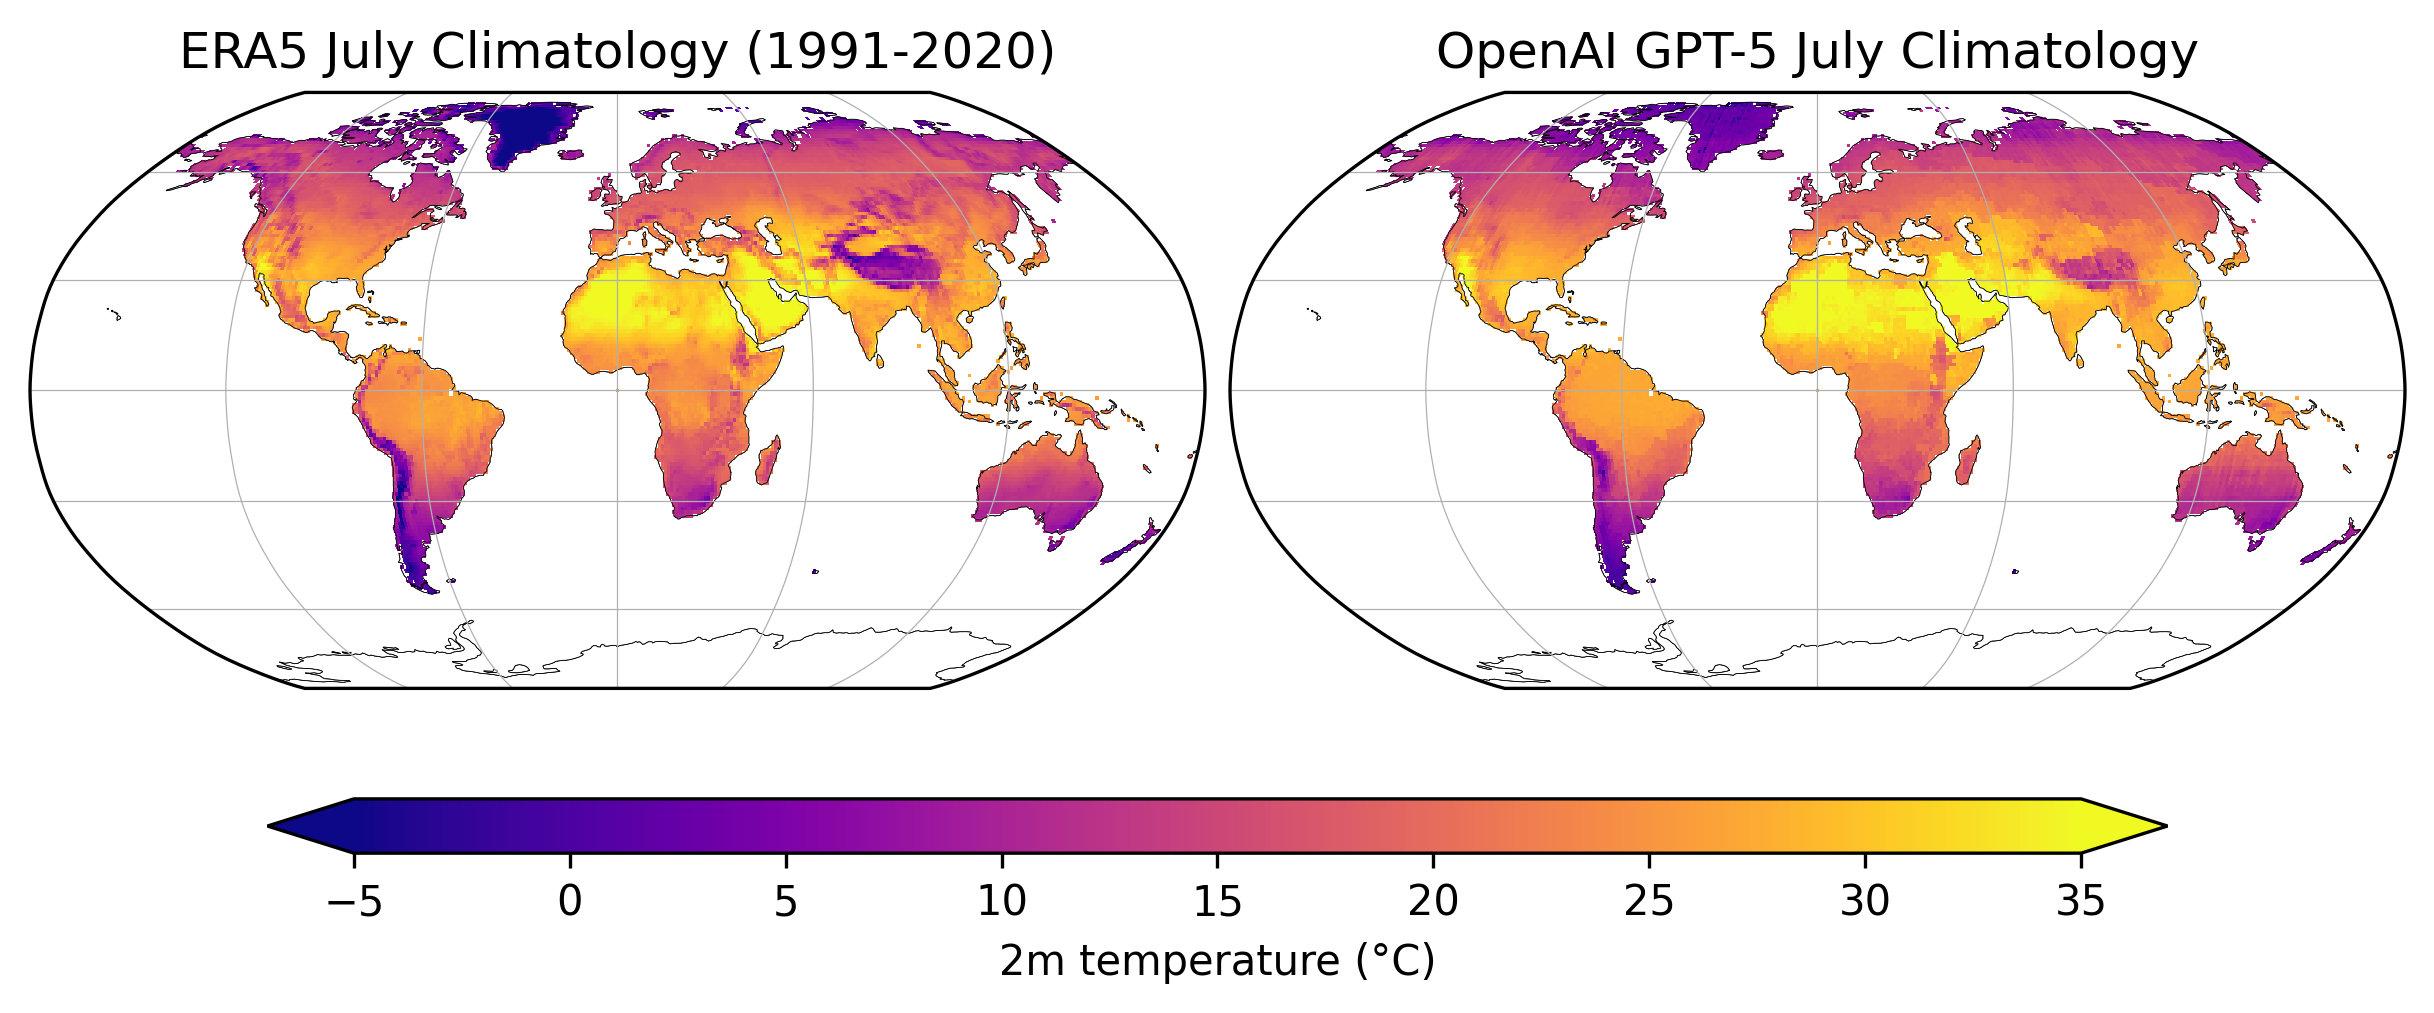
\includegraphics[width=1\linewidth]{Chapter4//figs/example_map.png}
    \caption{Mean July 2-m air temperature (1991-2020) from ERA5 reanalysis (left) and LLM GPT-5 predictions (right). Both panels are shown on a 1° grid.}
    \label{fig:july-climatology}
\end{figure}

The comparison was extended to all the model configurations included in the benchmark. Figure~\ref{fig:temperature-bias-maps} presents the reconstructed climatologies and their differences from ERA5, while Table~\ref{tab:llm-temperature-performance} and Figure~\ref{fig:bias_rmse_scatter} summarizes their global RMSE and mean bias. Across the configurations, RMSE ranges from \(3.5\,^{\circ}\mathrm{C}\) for GPT-5 to \(10.2\,^{\circ}\mathrm{C}\) for ClimateGPT 70B, with a median close to \(5\,^{\circ}\mathrm{C}\). Most models fall within the range of 3--\(6\,^{\circ}\mathrm{C}\). Changes in the sampling temperature have a much smaller effect. Moving from deterministic generation to a sampling temperature of 0.3 produces only marginal and inconsistent variations.

\begin{figure}[H]
    \centering
    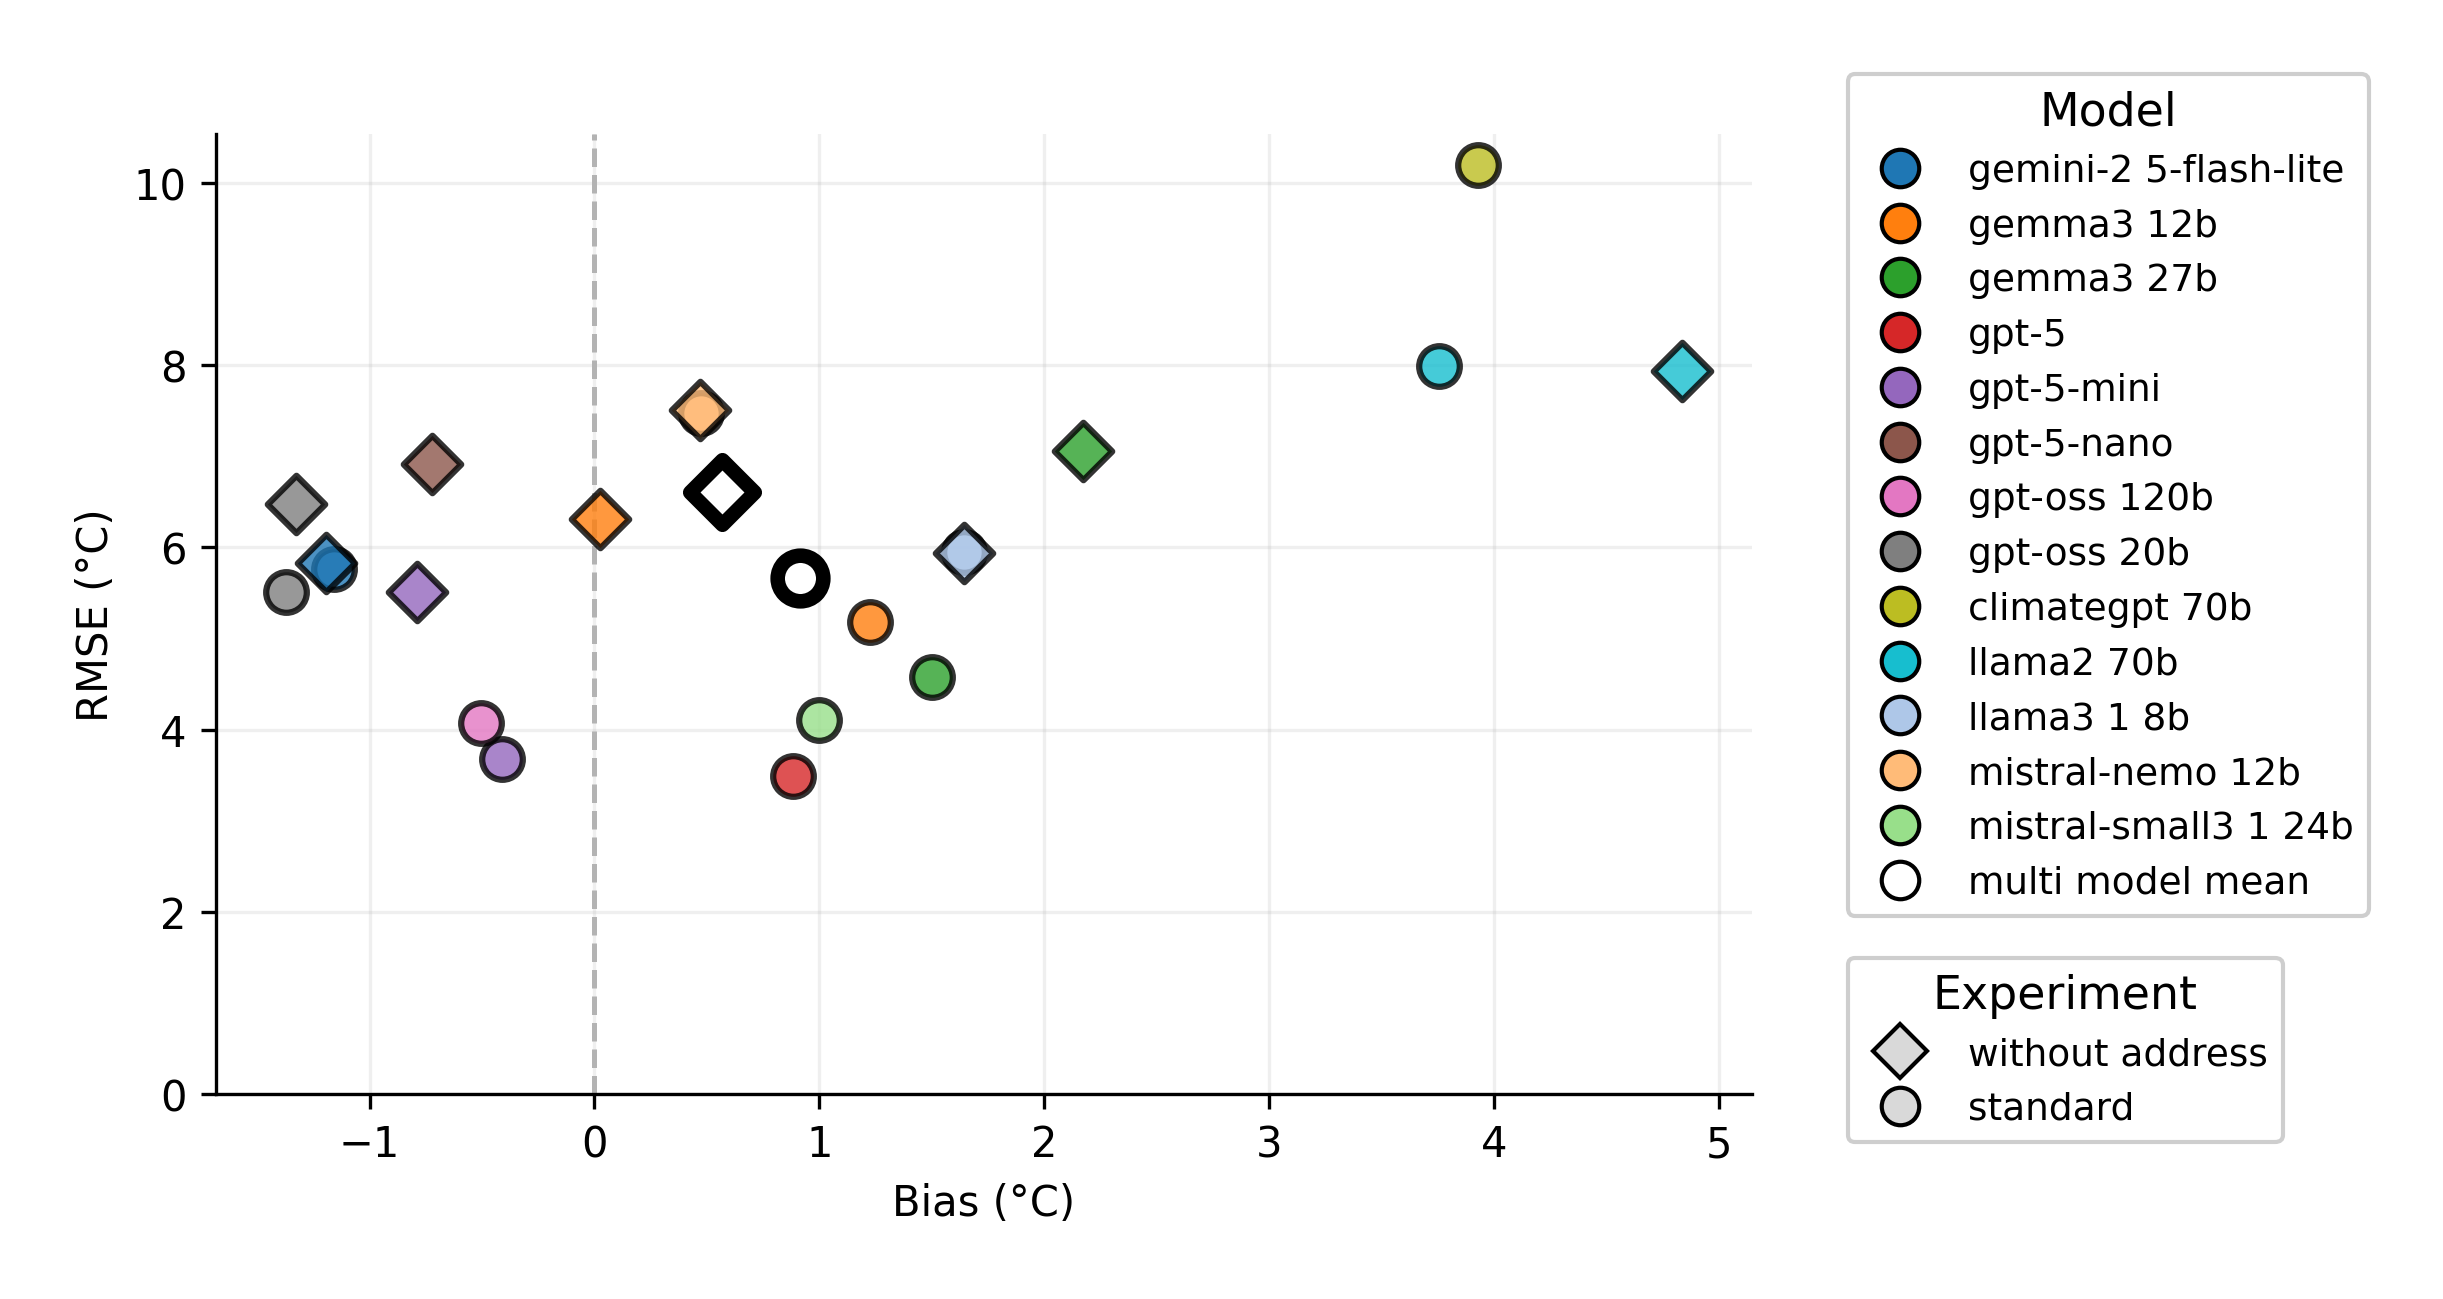
\includegraphics[width=1\linewidth]{Chapter4//figs/bias_rmse_scatter.png}
    \caption{Root-mean-square error (RMSE) against mean bias for LLM temperature
    predictions. All values are expressed in \(^{\circ}\mathrm{C}\). Only the simulation with \emph{temperature}=0 are shown, since setting \emph{temperature}=3 only produces small variations.}
    \label{fig:bias_rmse_scatter}
\end{figure}

The experiments show that the geographical information included in the prompt has a substantial influence on the results. Removing country, region, and city increases RMSE by an average of 27\%. For GPT-5 Mini, the error increases from 3.7 to \(5.6\,^{\circ}\mathrm{C}\); for Gemma 27B, it increases from 4.5 to \(7.1\,^{\circ}\mathrm{C}\); and for GPT-5 Nano, from 5.2 to \(6.9\,^{\circ}\mathrm{C}\). In contrast, some smaller models, including LLaMA 3.1 8B and Mistral Nemo 12B, show little sensitivity to the additional descriptors. This result suggests that coordinates alone are not an effective key to the climate information stored in many LLMs. Place names provide recognizable linguistic anchors that connect the query to geographical and climatic descriptions encountered during training. 

Mean biases are smaller than the corresponding RMSE values, since regional errors of opposite sign partly compensate when averaged over the global domain. Among the best configurations, they range from approximately \(-0.6\) to \(+0.9\,^{\circ}\mathrm{C}\), while the complete ensemble spans from \(-1.4\) to \(+4.8\,^{\circ}\mathrm{C}\). Interestingly, the sign of the bias also remains generally stable when the sampling configuration or the amount of geographical information in the prompt is changed, suggesting that warm or cold tendencies are characteristic of the models rather than consequences of individual prompt formulations.

% Prima pagina: pannelli (a)--(f)
\begin{figure}[p]
    \centering

    \mapmodel
        {Chapter4/figs/OpenAI GPT-5_map.png}
        {GPT-5}
    \hfill
    \mapmodel
        {Chapter4/figs/OpenAI GPT-5 Mini_map.png}
        {GPT-5 Mini}

    \medskip

    \mapmodel
        {Chapter4/figs/OpenAI GPT-5 Nano_map.png}
        {GPT-5 Nano}
    \hfill
    \mapmodel
        {Chapter4/figs/OpenAI GPT-OSS 20B_map.png}
        {GPT-OSS 20B}

    \medskip

    \mapmodel
        {Chapter4/figs/OpenAI GPT-OSS 120B_map.png}
        {GPT-OSS 120B}
    \hfill
    \mapmodel
        {Chapter4/figs/Gemini 2.5 Flash Lite_map.png}
        {Gemini 2.5 Flash Lite}

    \medskip
    
    \mapmodel
        {Chapter4/figs/Gemma3 12B_map.png}
        {Gemma 3 12B}
    \hfill
    \mapmodel
        {Chapter4/figs/Gemma3 27B_map.png}
        {Gemma 3 27B}

    

    \caption{
        Continues in the next page $\rightarrow$
    }
    \label{fig:temperature-bias-maps}
\end{figure}

% Seconda pagina: pannelli (g)--(m)
\begin{figure}[p]
    \ContinuedFloat
    \centering


    \mapmodel
        {Chapter4/figs/Mistral Nemo 12B_map.png}
        {Mistral Nemo 12B}
    \hfill
    \mapmodel
        {Chapter4/figs/Mistral Small3.1 24B_map.png}
        {Mistral Small 3.1 24B}

    \medskip

    \mapmodel
        {Chapter4/figs/LLaMA 2 70B_map.png}
        {LLaMA 2 70B}
    \hfill
    \mapmodel
        {Chapter4/figs/ClimateGPT 70B_map.png}
        {ClimateGPT 70B}

    \medskip

    \mapmodel
        {Chapter4/figs/LLaMA 3 1.8B_map.png}
        {LLaMA 3.1 8B}

    \caption[]{
        Spatial distribution of the July 2 m temperature bias relative to ERA5 for all the 13 models for the period 1991-2020. Only the configuration with \emph{temperature}=0 is reported, since setting \emph{temperature}=0 only produces small variations.
    }
\end{figure}

% Tabella risultati generali
\begin{longtable}{@{}lcc@{}}
    \caption{
        Root-mean-square error (RMSE) and mean bias for LLM temperature
        predictions. All values are expressed in \(^{\circ}\mathrm{C}\).
    }
    \label{tab:llm-temperature-performance}\\

    \toprule
    \textbf{Model/configuration}
    & \textbf{RMSE/bias (\(^{\circ}\mathrm{C}\))}
    & \textbf{RMSE/bias (\(^{\circ}\mathrm{C}\)) (No address)} \\
    \midrule
    \endfirsthead

    \multicolumn{3}{c}{%
        \tablename\ \thetable{} -- continued from previous page
    }\\
    \toprule
    \textbf{Model/configuration}
    & \textbf{RMSE/bias (\(^{\circ}\mathrm{C}\))}
    & \textbf{RMSE/bias (\(^{\circ}\mathrm{C}\)) (No address)} \\
    \midrule
    \endhead

    \midrule
    \multicolumn{3}{r}{Continued on next page}\\
    \endfoot

    \bottomrule
    \endlastfoot

    GPT-5, \(T=0.3\)
        & \(3.5 / 0.9\)
        & -- \\

    GPT-5 Mini, \(T=0.3\)
        & \(3.7 / {-0.4}\)
        & \(5.6 / {-0.8}\) \\

    GPT-5 Mini
        & \(3.7 / {-0.4}\)
        & -- \\

    GPT-OSS 120B, \(T=0.3\)
        & \(3.7 / {-0.6}\)
        & \(5.3 / {-0.6}\) \\

    GPT-OSS 120B
        & \(4.0 / {-0.4}\)
        & -- \\

    Mistral Small 3.1 24B, \(T=0.3\)
        & \(4.1 / 1.0\)
        & -- \\

    Mistral Small 3.1 24B
        & \(4.1 / 1.0\)
        & -- \\

    Gemma 27B, \(T=0.3\)
        & \(4.5 / 1.3\)
        & \(7.1 / 2.2\) \\

    Gemma 27B
        & \(4.6 / 1.5\)
        & -- \\

    GPT-OSS 20B, \(T=0.3\)
        & \(5.1 / {-1.3}\)
        & \(6.5 / {-1.3}\) \\

    Gemma 12B, \(T=0.3\)
        & \(5.2 / 1.1\)
        & -- \\

    Gemma 12B
        & \(5.2 / 1.2\)
        & \(6.3 / 0.0\) \\

    GPT-5 Nano, \(T=0.3\)
        & \(5.3 / {-0.8}\)
        & -- \\

    GPT-5 Nano
        & \(5.2 / {-0.8}\)
        & \(6.9 / {-0.7}\) \\

    GPT-OSS 20B
        & \(5.5 / {-1.4}\)
        & -- \\

    Gemini 2.5 Flash Lite, \(T=0.3\)
        & \(5.5 / {-1.2}\)
        & \(5.6 / {-1.2}\) \\

    Gemini 2.5 Flash Lite
        & \(5.8 / {-1.2}\)
        & \(5.8 / {-1.2}\) \\

    LLaMA 3.1 8B, \(T=0.3\)
        & \(5.9 / 1.8\)
        & \(5.9 / 1.8\) \\

    LLaMA 3.1 8B
        & \(6.0 / 1.6\)
        & \(5.9 / 1.6\) \\

    Mistral Nemo 12B, \(T=0.3\)
        & \(6.9 / 0.4\)
        & \(6.9 / 0.4\) \\

    Mistral Nemo 12B
        & \(7.5 / 0.5\)
        & \(7.5 / 0.5\) \\

    LLaMA 2 70B
        & \(8.0 / 3.8\)
        & \(7.9 / 4.8\) \\

    ClimateGPT 70B
        & \(10.2 / 3.9\)
        & -- \\

\end{longtable}

Model size provides a partial explanation for the differences in the performances. Within the same family, larger models generally perform better. GPT-5 and GPT-5 Mini outperform GPT-5 Nano, while GPT-OSS 120B improves on GPT-OSS 20B. However, this relationship does not hold across different model generations: LLaMA 3.1 8B outperforms the substantially larger LLaMA 2 70B by approximately \(2\,^{\circ}\mathrm{C}\). Model architecture, training data, and training procedure therefore appear to be at least as important as parameter count.

Domain specialization does not produce an advantage in this task. ClimateGPT 70B obtains the largest error in the ensemble, with an RMSE of \(10.2\,^{\circ}\mathrm{C}\), compared with \(8.0\,^{\circ}\mathrm{C}\) for the general-purpose LLaMA 2 70B from which it was derived. ClimateGPT was developed primarily for text-based climate question answering supported by retrieval, rather than for unaided numerical recall. Nevertheless, this comparison demonstrates that continued training on climate-related text does not necessarily improve the representation of quantitative climatological values and may alter numerical associations acquired by the original model.

The error maps show that he deviations are spatially coherent (Figure \ref{fig:temperature-bias-maps}). GPT-5 exhibits cold biases over parts of central Asia and South America and warm biases over Greenland and some areas of the Sahara. GPT-OSS 120B presents similarly coherent structures, although their sign differs in some regions. Mistral Small 3.1 24B and Gemma 27B show predominantly warm biases across large parts of the Northern Hemisphere mid-latitudes and colder biases in parts of the Southern Hemisphere.

A common feature across the models is the presence of particularly large errors over complex terrain. The Himalayas, the Tibetan Plateau, Greenland, the Andes, and other major mountain regions are systematically warmer in the LLM reconstructions than in ERA5. In these areas, the models reproduce the broad presence of a cold region but fail to represent the full magnitude of elevation cooling. By contrast, errors tend to be smaller over low-lying and densely populated areas.

The dependence on elevation is quantified in Table~\ref{tab:errors-by-altitude}, for four representative models. At elevations below 500 m, which contain 60.5\% of the evaluated land points, RMSE ranges from 1.9 to \(3.1\,^{\circ}\mathrm{C}\) across the four selected models. The error increases progressively with altitude, reaching 3.1--\(4.2\,^{\circ}\mathrm{C}\) between 1000 and 1500 m. A more pronounced deterioration occurs above 1500 m, where RMSE rises to 4.3--\(6.2\,^{\circ}\mathrm{C}\), depending on the model.

Above 2500 m, errors exceed \(7\,^{\circ}\mathrm{C}\) for all four models and are accompanied by warm biases ranging from approximately \(5\) to \(13\,^{\circ}\mathrm{C}\). Although only a relatively small fraction of the grid is located at these elevations, these points contribute disproportionately to the global error. Conversely, approximately 90\% of the evaluated locations lie below 1500 m, where the models perform considerably better. It is worth noting that ERA5, which is used here as the reference dataset, also has known limitations in representing data-sparse and high-elevation regions \citep{delhasse_brief_2020,munoz-sabater_era5-land_2021}. Therefore, the observed discrepancies cannot be attributed entirely to errors in the LLM estimates, as part of them may also reflect uncertainties in the reference data.

% Tabella risultati quota
\begin{table}[H]
    \centering
    \caption{
        RMSE and bias by altitude band for the selected models.
        The percentages indicate the fraction of grid cells belonging
        to each altitude band. All values are expressed in \(^{\circ}\mathrm{C}\).
    }
    \label{tab:errors-by-altitude}

    \resizebox{\textwidth}{!}{%
    \begin{tabular}{lrrrrrrrr}
        \toprule
        & \multicolumn{2}{c}{GPT-5}
        & \multicolumn{2}{c}{GPT-OSS 120B}
        & \multicolumn{2}{c}{Mistral Small 3.1 24B}
        & \multicolumn{2}{c}{Gemma 3 27B} \\
        \cmidrule(lr){2-3}
        \cmidrule(lr){4-5}
        \cmidrule(lr){6-7}
        \cmidrule(lr){8-9}

        \textbf{Altitude band}
        & \textbf{RMSE} & \textbf{Bias}
        & \textbf{RMSE} & \textbf{Bias}
        & \textbf{RMSE} & \textbf{Bias}
        & \textbf{RMSE} & \textbf{Bias} \\
        \midrule

        0--500 m (60.5\%)
        & 1.9 & -0.1
        & 3.1 & -1.4
        & 3.0 &  0.0
        & 3.1 &  0.2 \\

        500--1000 m (19.2\%)
        & 2.3 &  0.6
        & 3.3 & -0.3
        & 3.4 &  0.8
        & 3.3 &  1.1 \\

        1000--1500 m (10.3\%)
        & 3.1 & 1.5
        & 3.4 & 0.2
        & 3.9 & 1.9
        & 4.2 & 2.0 \\

        1500--2000 m (3.9\%)
        & 5.2 & 3.8
        & 4.3 & 0.9
        & 4.8 & 3.1
        & 6.2 & 4.1 \\

        2000--2500 m (2.3\%)
        & 8.5  & 7.3
        & 5.6  & 3.0
        & 7.0  & 5.8
        & 10.3 & 8.8 \\

        2500--3000 m (1.4\%)
        & 11.7 & 10.6
        & 7.4  & 5.1
        & 8.6  & 7.7
        & 14.1 & 12.8 \\

        3000--3500 m (0.6\%)
        & 12.4 & 10.9
        & 9.5  & 7.0
        & 11.7 & 10.4
        & 14.0 & 12.3 \\

        3500--4000 m (0.5\%)
        & 11.2 & 8.6
        & 10.3 & 5.4
        & 12.7 & 11.0
        & 11.5 & 9.7 \\

        \(>4000\) m (1.5\%)
        & 11.3 & 9.5
        & 9.5  & 5.7
        & 13.9 & 12.8
        & 11.6 & 9.2 \\

        \bottomrule
    \end{tabular}%
    }
\end{table}



As a last observation, the magnitude of some LLM errors is comparable to biases found when physical climate models are evaluated against reanalysis at similar spatial scales \citep{eyring_overview_2016}. This comparison provides a useful numerical reference but does not imply equivalence between the two types of model. Climate model errors arise from approximations in the representation of physical processes and boundary conditions, whereas LLM errors reflect incomplete or uneven statistical associations in their training material. Similar error magnitudes therefore have fundamentally different interpretations.




Overall, the experiment reveals a clear distinction between geographical plausibility and local quantitative reliability. Current LLMs encode enough climate information to reconstruct the broad spatial organization of July temperature and, in favorable conditions, to provide reasonable estimates for low-elevation and well-documented locations. Their errors nevertheless increase markedly where local temperature depends on geographical details that are not reliably represented in textual training data. The strong contribution of place names and the systematic difficulty over high terrain indicate that this capability should be interpreted as parametric recall supported by geographical associations, rather than as evidence of an internal physical model of the climate system.

\subsection{Climate Knowledge Across the Seasonal Cycle}

The previous analysis showed that LLMs encode a recognizable representation of the geographical distribution of July temperature. However, a single month cannot establish whether this knowledge extends to the complete annual cycle. To test this, the evaluation was repeated for all twelve calendar months using GPT-5, GPT-OSS 120B, Mistral Small 3.1 24B, and Gemma 27B. The experiment was conducted on the subset of 1,540 land points described in the previous section, with each model asked to return the twelve monthly climatological temperatures in a single response.

The extension to the annual cycle broadly confirms the conclusions obtained from the July experiment. As shown in Figure~\ref{fig:monthly-rmse}, the relative ranking of the four models is preserved across the year. When evaluated over all 18,480 point-month combinations, GPT-5 achieves the lowest RMSE, \(3.73\,^{\circ}\mathrm{C}\), followed by GPT-OSS 120B with \(4.00\,^{\circ}\mathrm{C}\), Mistral Small 3.1 24B with \(4.94\,^{\circ}\mathrm{C}\), and Gemma 27B with \(6.10\,^{\circ}\mathrm{C}\). The ability to reproduce the July climatology is therefore not an isolated result, but reflects a more general representation of the seasonal temperature cycle.

GPT-5 also exhibits the most stable performance throughout the year. Its monthly RMSE ranges from \(3.46\) to \(4.09\,^{\circ}\mathrm{C}\), with a mean annual bias of \(-0.33\,^{\circ}\mathrm{C}\). The other three models are warm-biased when evaluated across the full annual cycle, with biases ranging from \(+0.86\) to \(+1.77\,^{\circ}\mathrm{C}\). Their errors also display a more pronounced seasonal dependence, generally increasing during boreal autumn. Mistral Small 3.1 24B reaches an RMSE of \(6.22\,^{\circ}\mathrm{C}\) in November, while Gemma 27B reaches \(7.14\,^{\circ}\mathrm{C}\) in October.

These results indicate that the models encode the broad timing and direction of the seasonal cycle, including the reversal of seasons between the Northern and Southern Hemispheres. Nevertheless, the quantitative errors remain substantial. The ERA5 interannual variability calculated at the same locations averages \(2.00\,^{\circ}\mathrm{C}\) over the year, with larger values during boreal winter and smaller values during boreal summer. The monthly errors produced by the LLMs are therefore typically two to three times larger than the natural year-to-year variability of monthly temperature. A model may consequently reproduce the general form of the seasonal cycle while still providing climatological values that are unreliable for quantitative local applications.

\begin{figure}[H]
    \centering
    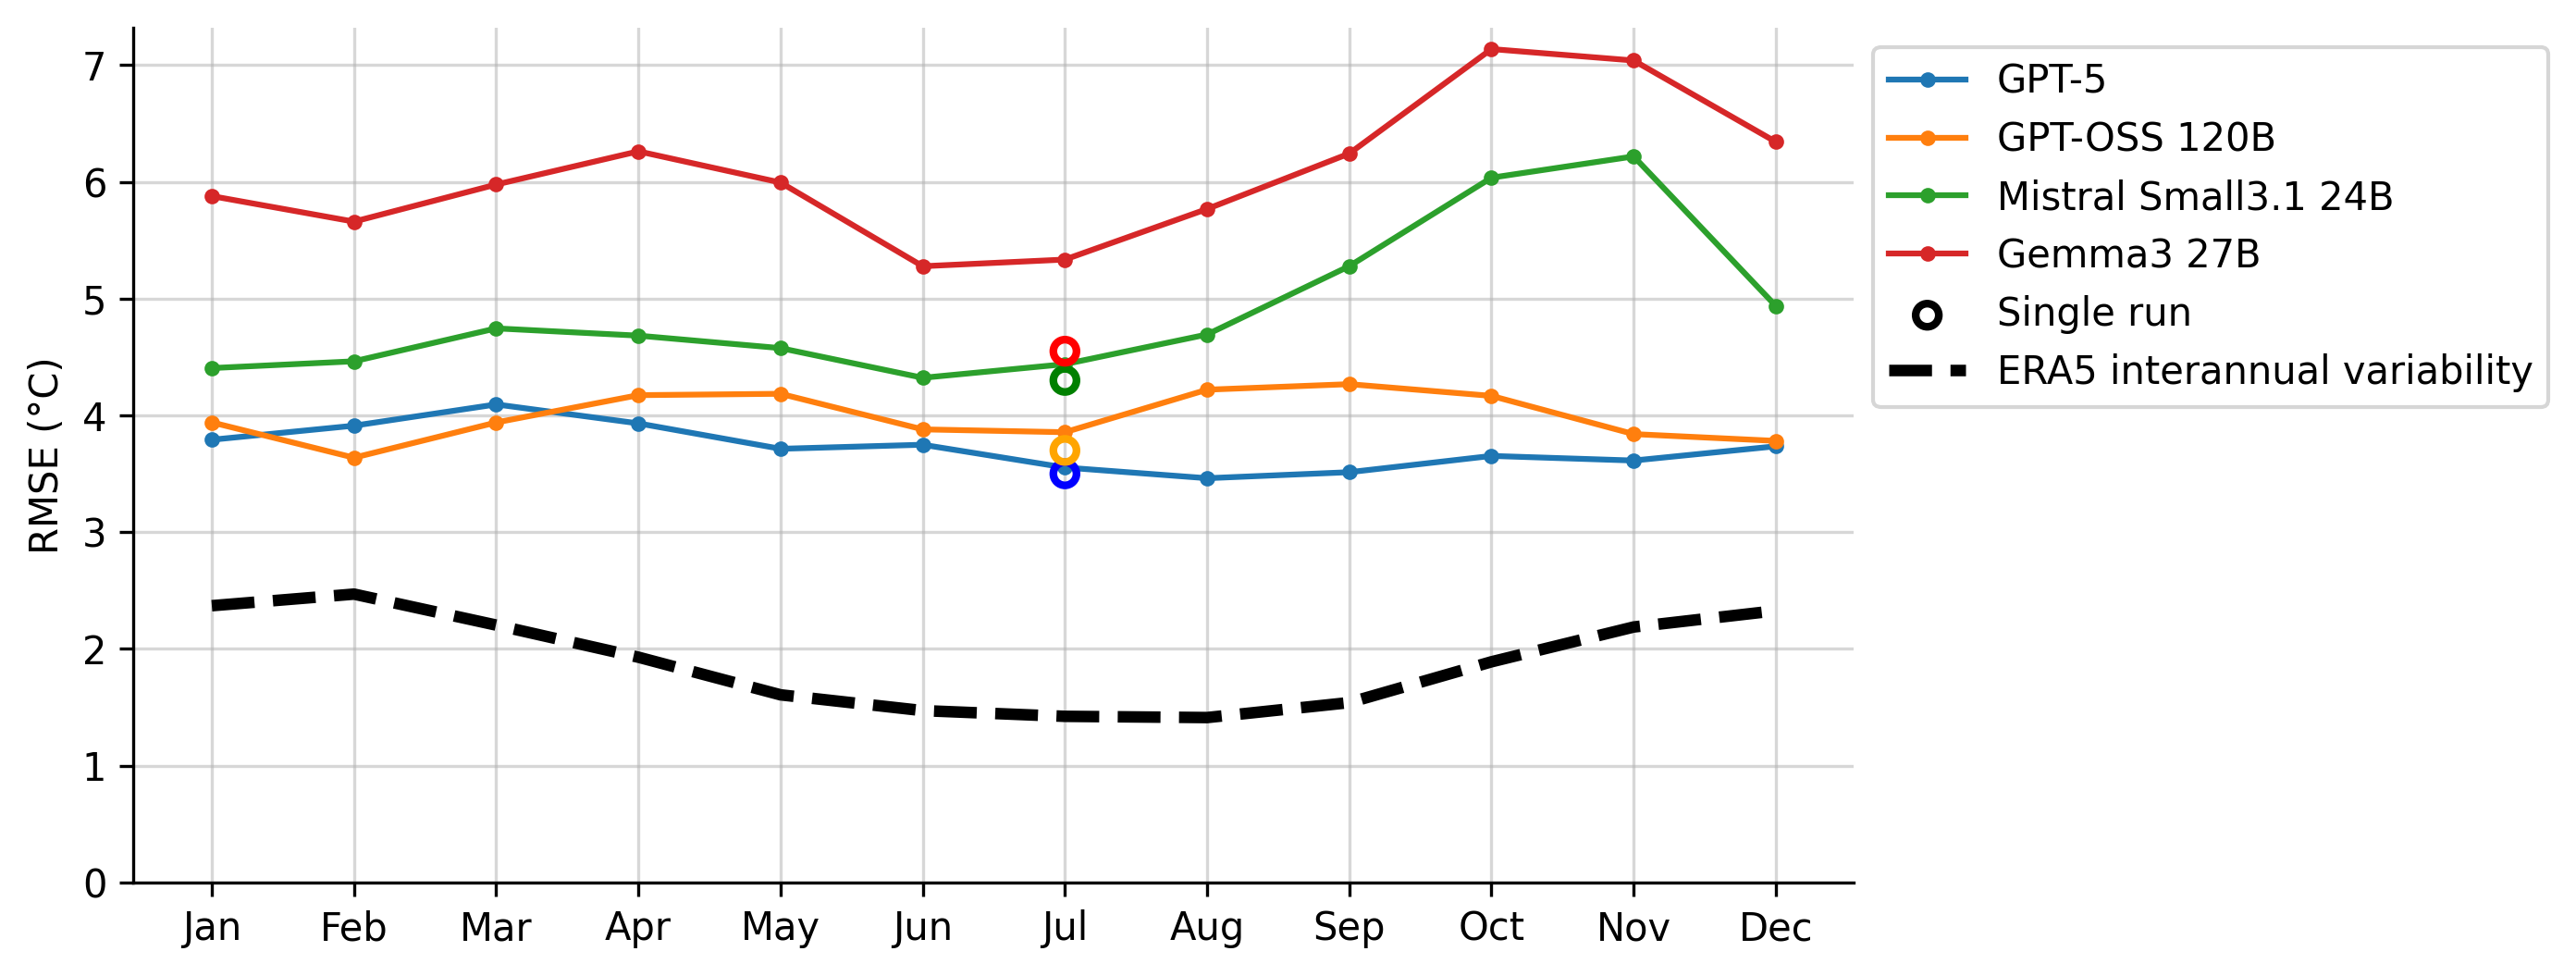
\includegraphics[width=\linewidth]{Chapter4/figs/seasonal_rmse.png}
    \caption{
        Monthly RMSE of closed-book LLM predictions of mean 2-m air temperature for 1991--2020 against ERA5. Results are shown for GPT-5, GPT-OSS 120B, Mistral Small 3.1 24B, and Gemma 27B at 1,540 land points. The dashed black line represents ERA5 interannual variability, while open circles show the corresponding results obtained from independent single month queries. All LLM experiments shown here use the default sampling configuration of the respective API.
    }
    \label{fig:monthly-rmse}
\end{figure}

Part of the difference between the July and annual experiments may be related to the structure of the query itself. In the main benchmark, the models were asked to provide only the July temperature. In the seasonal experiment, they had to return twelve coherent values in the same response. To separate the effect of this additional task complexity from differences in stored climatological information, the July value extracted from the joint twelve-month query was compared with the result of an independent single-month July query.

For GPT-5, the two formulations produce nearly identical results: the July RMSE is \(3.55\,^{\circ}\mathrm{C}\) in the joint query and \(3.59\,^{\circ}\mathrm{C}\) in the single-month query. The joint query increases RMSE by approximately \(0.2\,^{\circ}\mathrm{C}\) for GPT-OSS 120B and Mistral Small 3.1 24B. The largest difference is observed for Gemma 27B, whose July RMSE increases from \(4.55\) to \(5.34\,^{\circ}\mathrm{C}\). The weaker model is therefore more sensitive to the requirement of producing a complete and internally coherent annual cycle.

This comparison suggests that the seasonal errors combine two distinct limitations. The first concerns the climate information represented in the model parameters. The second concerns the ability of the model to retrieve and organize several related numerical values within a single response. This distinction is relevant for Climate Services, where LLMs may be required to communicate complete time series or sets of indicators rather than isolated values.

The robustness of these conclusions was further evaluated with respect to the sampling configuration and the reduced spatial domain. Figure~\ref{fig:sampling-sensitivity} compares the July results obtained using sampling temperatures of 0 and 0.3 with those obtained using the default setting of each API. Across the four models, changing the sampling configuration modifies RMSE by no more than \(0.45\,^{\circ}\mathrm{C}\) and mean bias by no more than \(0.18\,^{\circ}\mathrm{C}\). These changes are small compared with the differences between models.

GPT-OSS 120B shows the largest sensitivity, with RMSE decreasing from \(4.11\,^{\circ}\mathrm{C}\) under deterministic sampling to \(3.66\,^{\circ}\mathrm{C}\) using the API-default configuration. For the other three models, RMSE varies by \(0.15\,^{\circ}\mathrm{C}\) or less. The choice of sampling temperature therefore has only a secondary influence on the estimated climate knowledge and does not alter the relative performance of the models.

\begin{figure}[H]
    \centering
    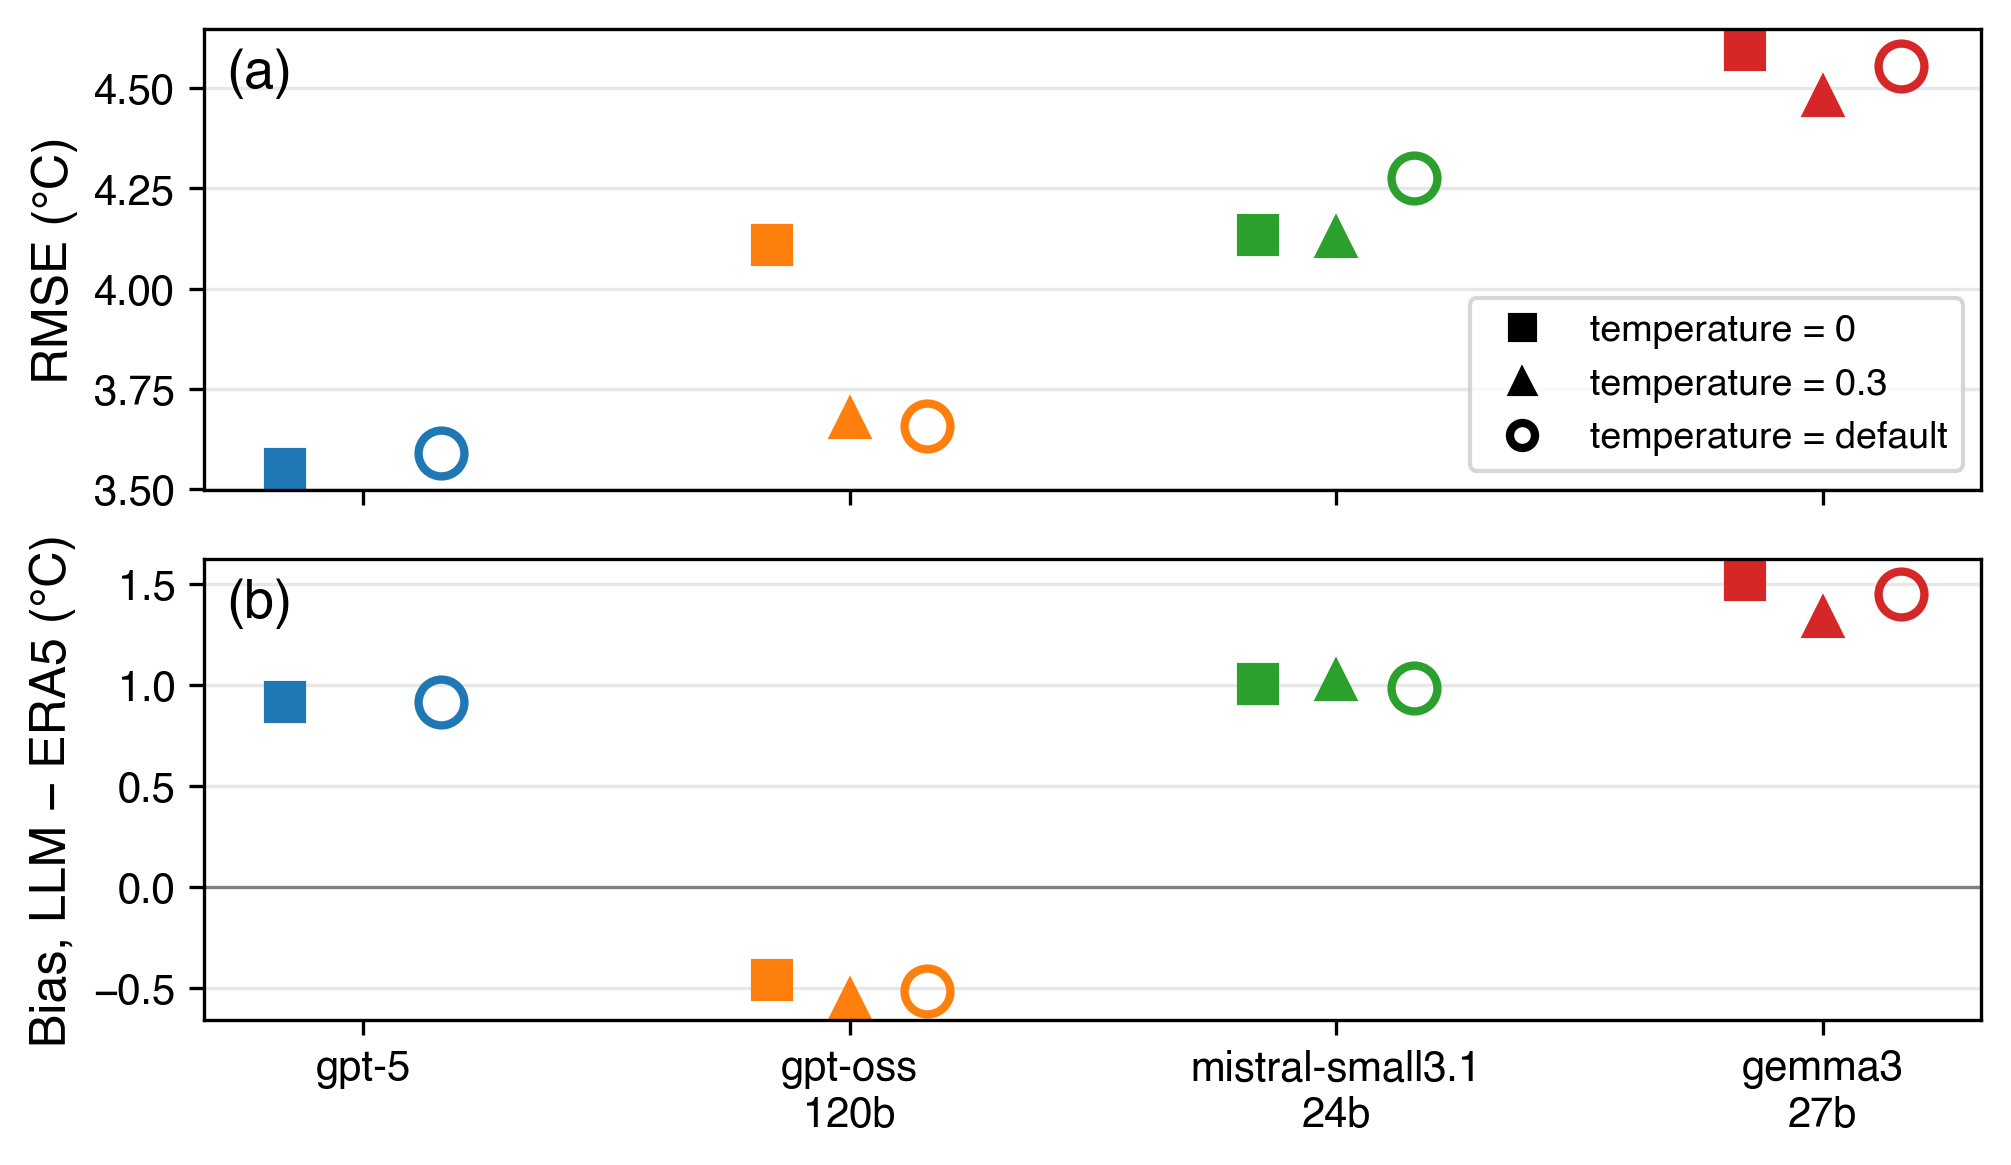
\includegraphics[width=0.75\linewidth]{Chapter4/figs/sampling_sensitivity.png}
    \caption{
        Sensitivity of July temperature performance to the sampling configuration on the 1,540-point subset. Panels show (a) RMSE and (b) mean bias relative to ERA5. Filled squares indicate sampling temperature 0, filled triangles indicate sampling temperature 0.3, and open circles indicate the default API configuration.
    }
    \label{fig:sampling-sensitivity}
\end{figure}

The subset used for the seasonal experiment also reproduces the results obtained over the complete global grid. At a sampling temperature of 0.3, GPT-OSS 120B has an RMSE of \(3.68\,^{\circ}\mathrm{C}\) on the subset and \(3.67\,^{\circ}\mathrm{C}\) on the complete grid. For Gemma 27B, the corresponding values are \(4.48\) and \(4.49\,^{\circ}\mathrm{C}\). The ten-percent subset can therefore be considered representative of the larger spatial experiment for the purpose of comparing monthly performance.

Overall, the seasonal extension reinforces the distinction between structural and quantitative climate knowledge. The evaluated LLMs reproduce the broad annual temperature cycle and maintain a relatively stable ranking across months. Their numerical errors, however, remain larger than the observed interannual variability, and weaker models become less reliable when several climatological values must be generated simultaneously. The results are robust to both the spatial subsampling and the sampling-temperature configuration, indicating that these limitations reflect the underlying models rather than specific experimental choices.




\subsection{Parametric Knowledge of Climate Change}

The previous experiments evaluated whether LLMs encode the present-day temperature climatology and its seasonal cycle. These quantities describe relatively stable characteristics of the climate system that are frequently associated with specific locations in textual sources. Representing climate change poses a different and more demanding problem. It requires the model not only to associate a location with a typical temperature, but also to distinguish between different historical periods and quantify how that temperature has changed over time.

To evaluate this capability, the models were asked to estimate the difference in mean July 2-m air temperature between 1950--1974 and 2000--2024. The resulting values were compared with the corresponding differences derived from ERA5. As in the previous experiments, the models operated in a closed-book setting and were not provided with external observations, reanalysis data, or time series from which the temperature change could be calculated. We repeated the experiment for GPT5, which acheved the best performances in the previous test, and Mistral Small 3.1 24b as representative of a small open source model.

At the global scale, the models reproduced the approximate magnitude of observed warming. The mean temperature change over ERA5 land points is \(1.05\,^{\circ}\mathrm{C}\), while GPT-5 estimates a global mean of approximately \(0.96\,^{\circ}\mathrm{C}\). Mistral Small 3.1 24B produces an average warming of approximately \(0.8\,^{\circ}\mathrm{C}\). These values indicate that information about the overall magnitude of recent global warming is represented in the parameters of the models.

This apparent agreement at the global level, however, does not extend to the geographical distribution of the change. Figure~\ref{fig:climate-change-map} compares the ERA5-derived temperature change with that estimated by GPT-5. The model produces some spatial variation, but the resulting pattern does not reproduce the regional structure found in ERA5. The agreement in the global mean therefore results from averaging geographically inconsistent estimates.

\begin{figure}[H]
    \centering
    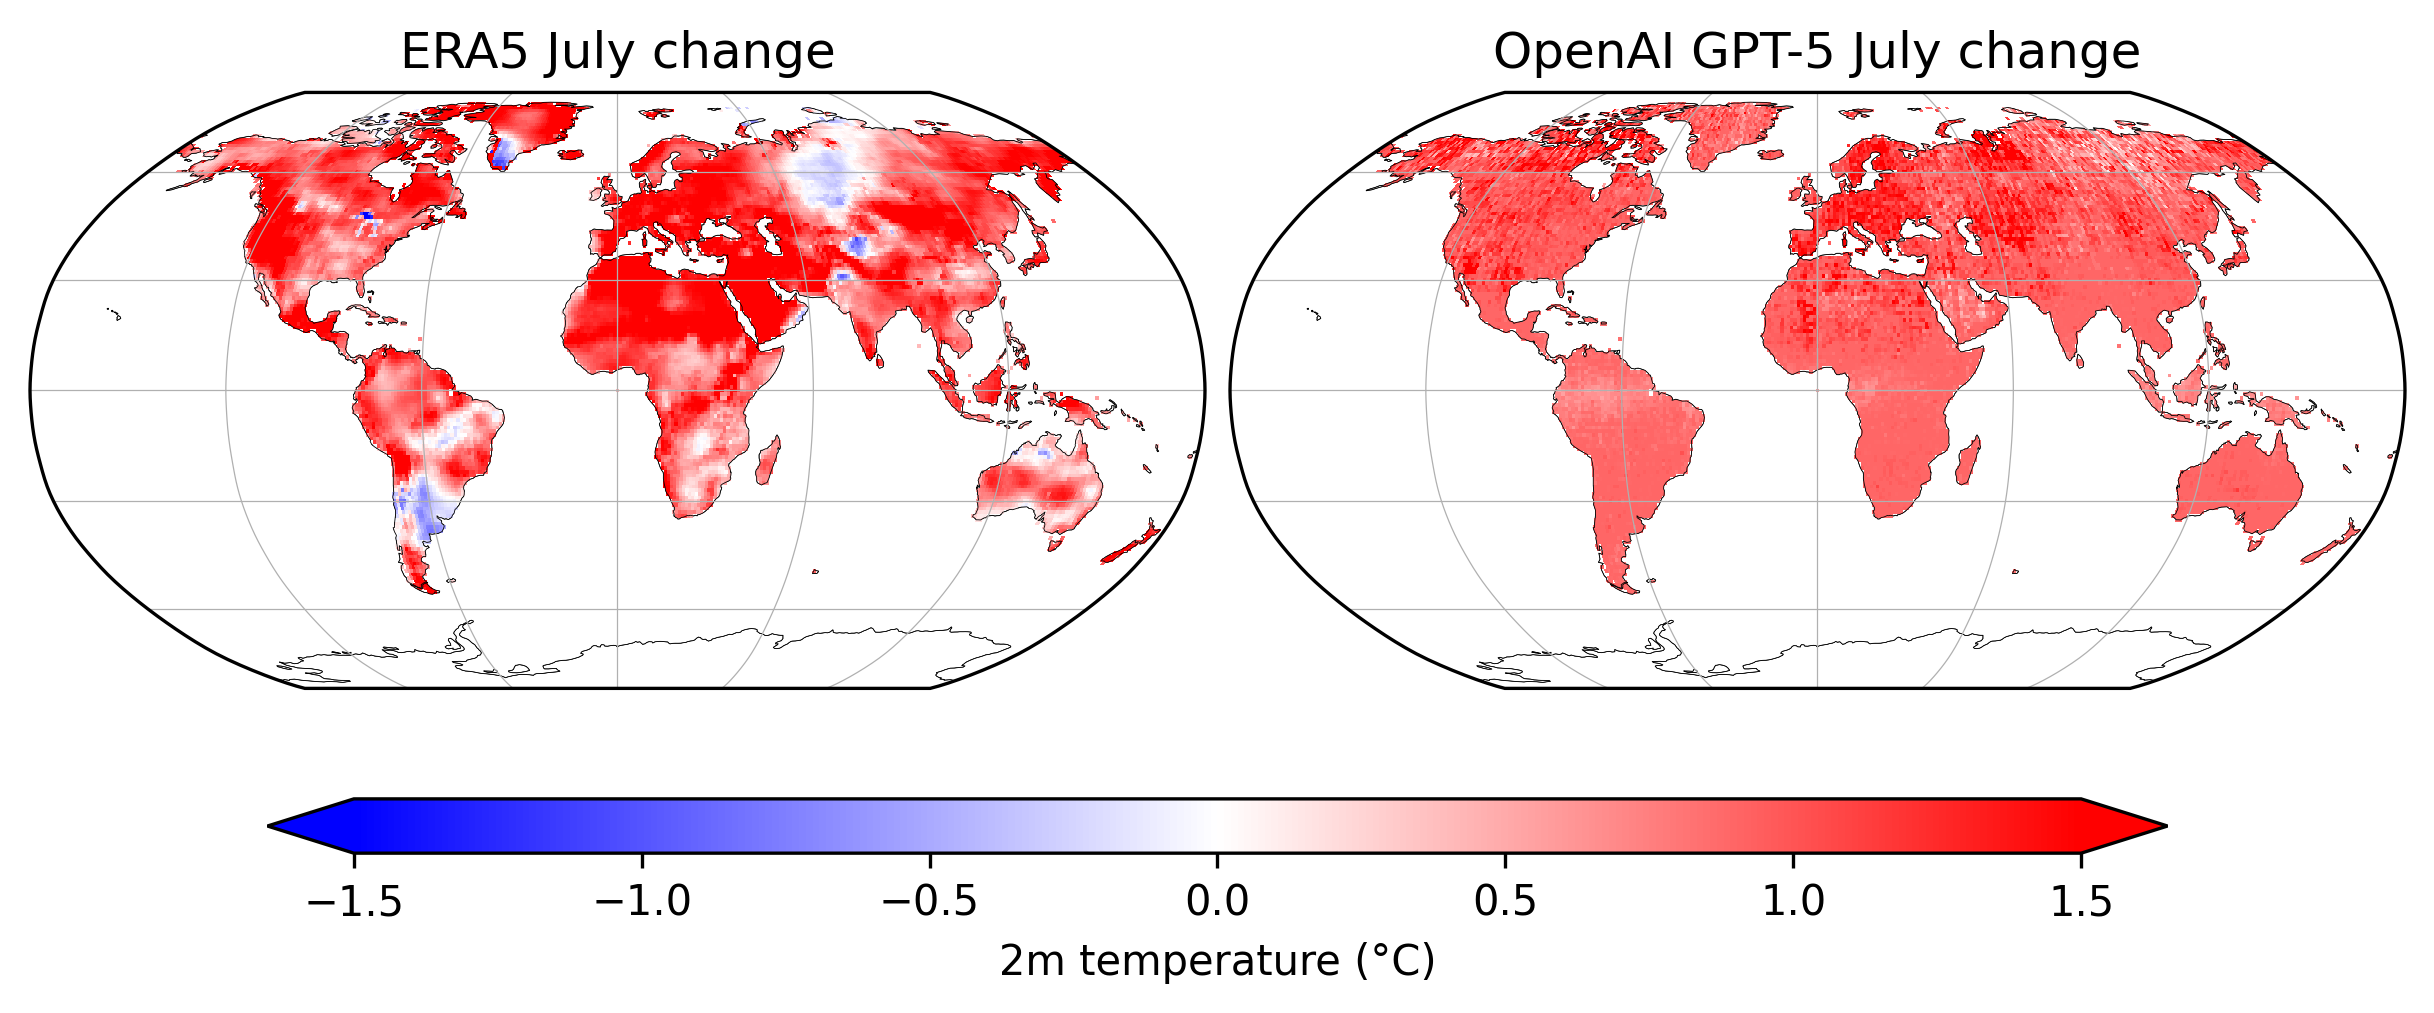
\includegraphics[width=0.75\linewidth]{Chapter4/figs/change_map.png}
    \caption{
        Change in mean July 2-m air temperature between 1950--1974
        and 2000--2024. The figure compares the change derived from
        ERA5 with the corresponding closed-book estimates produced
        by GPT-5.
    }
    \label{fig:climate-change-map}
\end{figure}

The spatial distribution of the errors for the two models is shown in Figure~\ref{fig:climate-change-bias}. Despite their different architectures, the models produce remarkably similar error patterns relative to ERA5. The absolute spatial correlation between each error field and the ERA5 change exceeds 0.90, whereas the change fields generated by the models correlate with ERA5 by less than 0.10. This occurs because both models produce nearly uniform warming maps centred around the approximate global mean value, with little meaningful regional variability. When these nearly constant estimates are compared with ERA5, the resulting error fields largely reproduce the spatial structure of the reference field, with the sign depending on the adopted bias convention. The similarity of the errors across models therefore does not indicate consistent geographical skill; rather, it reflects their common failure to represent the regional distribution of warming.

\begin{figure}[H]
    \centering
    \mapmodel
        {Chapter4/figs/change_bias_OpenAI GPT-5.png}
        {GPT-5}
    \hfill
    \mapmodel
        {Chapter4/figs/change_bias_Mistral Small 3.1 24b}
        {Mistral Small 3.1 24b}
    \caption{
        Spatial distribution of the bias in the estimated change in mean July 2-m air temperature between 1950--1974 and 2000--2024 for (a) GPT-5 and (b) Mistral Small 3.1 24B. Bias is defined as the LLM estimate minus the ERA5 change. The similar error patterns arise because both models produce nearly uniform warming fields, leaving the regional variability represented by ERA5 as the dominant structure in the residuals.
        }    
    \label{fig:climate-change-bias}
\end{figure}

The limitation is particularly evident for Mistral Small 3.1 24B, which returns an almost spatially uniform warming of approximately \(0.87\,^{\circ}\mathrm{C}\). GPT-5 estimates a similar global mean of \(0.96\,^{\circ}\mathrm{C}\), but produces a wider range of values across locations. In both cases, these averages are relatively close to the ERA5 land mean of \(1.05\,^{\circ}\mathrm{C}\), despite the poor correspondence of the individual grid-point estimates.

Figure~\ref{fig:q_q} separates the ability to reproduce the distribution of temperature changes from the ability to assign those changes to the correct locations. For GPT-5, the paired values show substantial variability around the global mean, and the quantile--quantile comparison indicates that the model reproduces part of the range found in ERA5. However, this distribution is compressed, particularly for the largest changes, and the weak point-wise relationship shows that the generated values are not associated with the correct geographical locations.

The limitation is more pronounced for Mistral Small 3.1 24B. Its paired values form an almost horizontal band around the model mean, while its quantiles vary only slightly across the much broader ERA5 distribution. The model therefore appears to apply approximately the same global warming value to almost every location. These results show that agreement in the global mean is not sufficient evidence of regional climate knowledge. GPT-5 generates some spatial variability without reproducing its geographical organization, whereas Mistral largely collapses the complete field towards a single global value.

\begin{figure}[H]
    \centering

    \begin{subfigure}{0.9\textwidth}
        \centering
        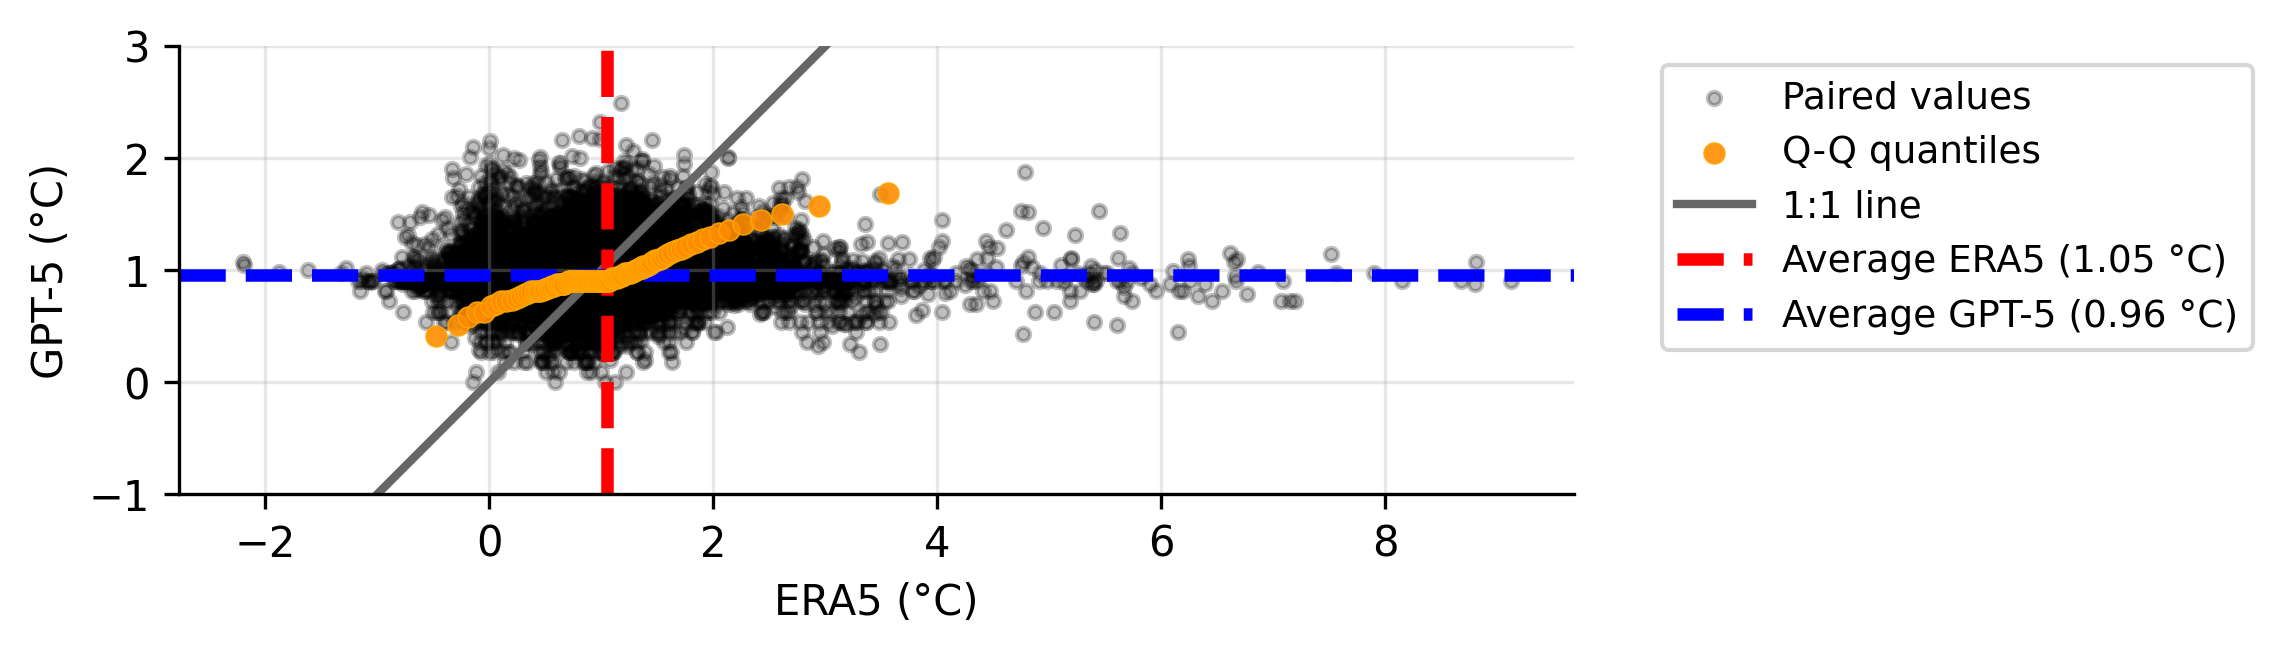
\includegraphics[width=\textwidth]{Chapter4/figs/change_q_q_OpenAI GPT-5.png}
        \caption{GPT-5}
        \label{fig:plot1}
    \end{subfigure}

    \vspace{0.5cm}

    \begin{subfigure}{0.9\textwidth}
        \centering
        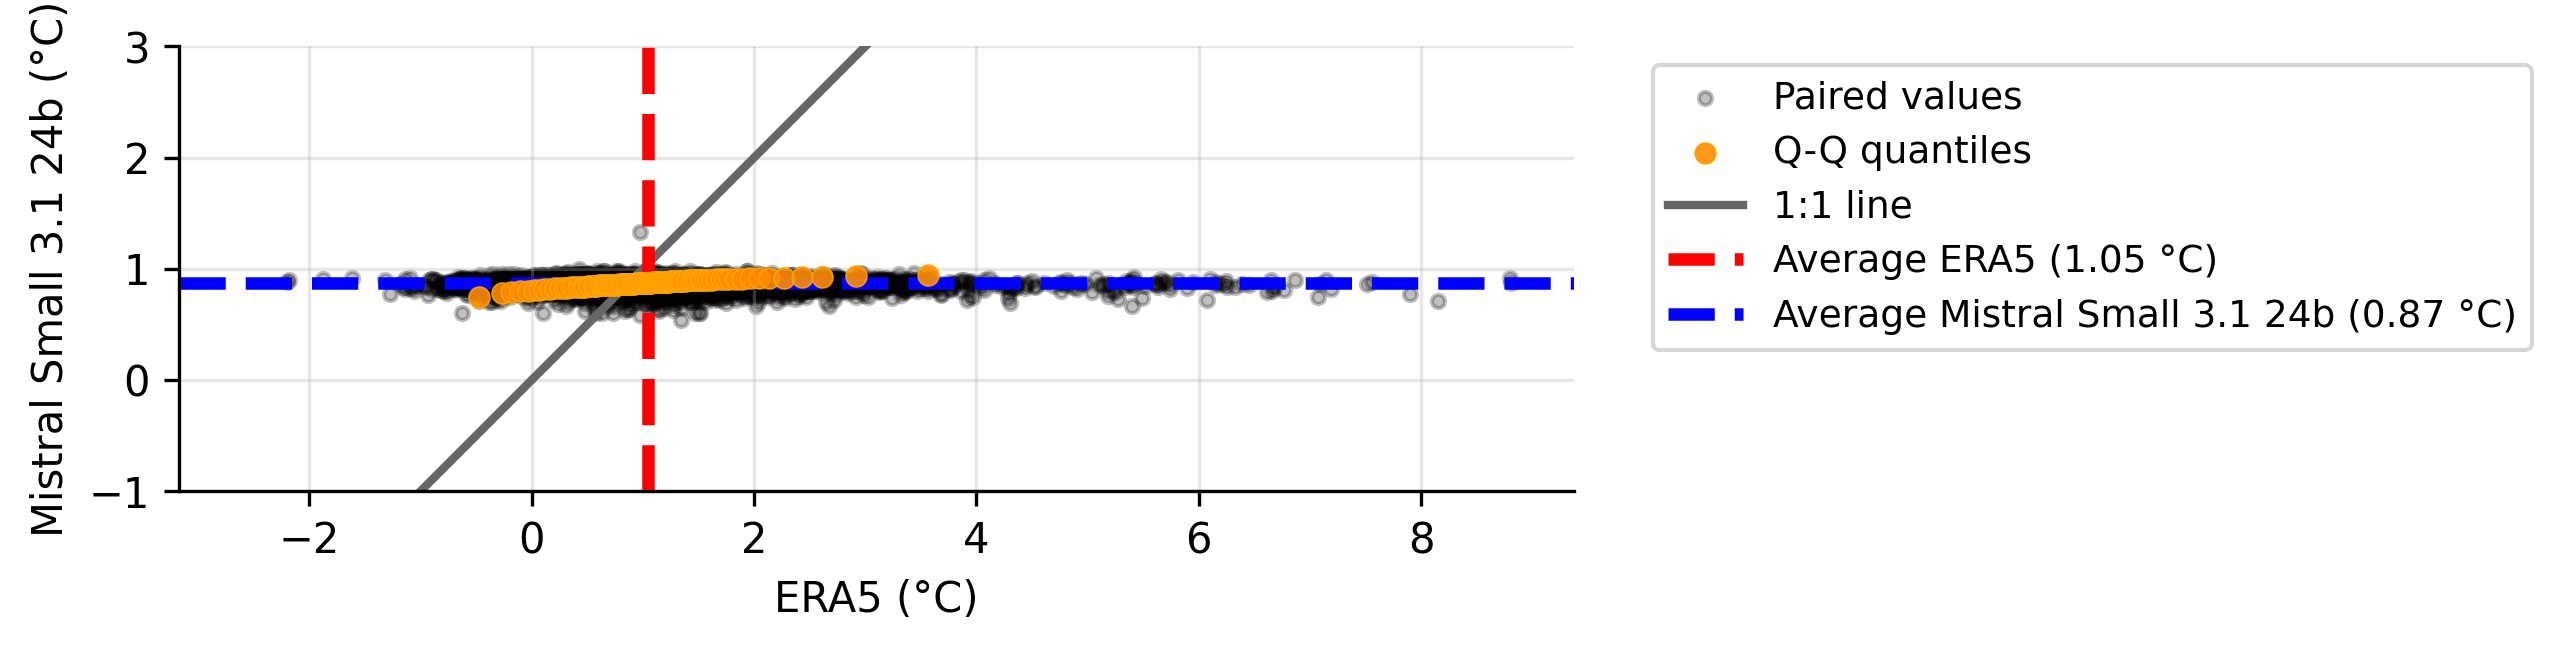
\includegraphics[width=\textwidth]{Chapter4/figs/change_q_q_Mistral Small 3.1 24b.png}
        \caption{Mistral Small 3.1 24b}
        \label{fig:plot2}
    \end{subfigure}

    \caption{
        Comparison between ERA5-derived and LLM-estimated changes in mean July 2-m air temperature between 1950--1974 and 2000--2024 for (a) GPT-5 and (b) Mistral Small 3.1 24B. Grey points show paired values at individual grid cells, while orange points compare the quantiles of the two distributions. The grey line represents perfect agreement, and the red and blue dashed lines indicate the ERA5 and LLM global means, respectively. GPT-5 produces a broader but compressed range of temperature changes, whereas Mistral Small 3.1 24B returns values strongly concentrated around its global mean.
        }
    \label{fig:q_q}
\end{figure}

A possible explanation for this difference between climatological means and climate change lies in how the relevant information is represented in textual training data. The present-day climate of a city or region is often described explicitly through statements about typical monthly temperatures. These statements can create direct associations between place names and climatological values. Local temperature changes, by contrast, are less frequently reported as explicit numerical facts and are more often contained in scientific datasets, figures, or specialized publications.

Reconstructing a local change would therefore require the model either to have encountered the exact value during training or to combine information referring to the same location at different times. The results provide no evidence that the evaluated LLMs can systematically perform this second operation. They do not appear to reconstruct an implicit local time series from separate pieces of information and then derive a consistent temperature difference from it.


\section{Discussion}

The experiments presented in this chapter provide a quantitative characterization of the climate information encoded in the parameters of contemporary LLMs. Taken together, the results reveal a consistent distinction between the ability to reproduce broad and frequently documented climatic regularities and the ability to provide accurate, geographically specific information. The models capture the general spatial organization of temperature, the annual cycle, and the approximate magnitude of global warming. Their reliability, however, decreases when the requested information depends on local geographical features or on the regional expression of temporal change.

This distinction is central to assessing the possible role of LLMs in Climate Services. A response may be globally plausible and linguistically convincing while remaining unsuitable for a local quantitative application.


\subsection{Parametric Recall versus Climate Understanding}

The ability of LLMs to reproduce the broad distribution of temperature demonstrates that their parameters contain a non-trivial representation of the Earth's climate. The models distinguish warm tropical and subtropical regions from colder high latitudes, reproduce the reversal of the seasonal cycle between hemispheres, and associate many locations with reasonable climatological values. This information is sufficiently structured to generate fields that resemble a physical climatology at the global scale.

However, these results should not be interpreted as evidence that LLMs possess an internal physical representation of the climate system. Unlike numerical climate models, they do not calculate temperature from governing equations, surface properties, atmospheric circulation, or energy exchanges. Their answers result from statistical associations learned during training. The fact that a generated field appears physically plausible does not establish whether the model has recalled an explicit value, combined multiple textual associations, or produced an estimate based on geographically related concepts.

The strong effect of geographical descriptors supports this interpretation. Adding country, region, and city names reduces RMSE by 27\% on average, even though the coordinates and the target location remain unchanged. Place names therefore appear to provide more effective access to parametric climate knowledge than numerical coordinates. This is consistent with the structure of textual training corpora, in which climate information is usually associated with recognizable geographical entities rather than latitude--longitude pairs. Widely documented locations consequently benefit from stronger linguistic associations, while remote, sparsely populated, and high-elevation regions are represented less reliably.

The errors over complex terrain further illustrate the difference between statistical recall and physical inference. An empirical or physically based model supplied with elevation could account for at least part of the expected temperature decrease with altitude. The evaluated LLMs instead produce increasingly warm estimates above 1500 m, despite correctly identifying many mountain regions as colder than their surroundings. They capture the qualitative association between mountains and lower temperatures but do not apply it with sufficient quantitative consistency.

The climate change experiment provides an even clearer example. The models reproduce the approximate magnitude of global warming, a value that is widely stated in scientific and public communication. They do not, however, reconstruct its regional distribution. Mistral Small 3.1 24B returns nearly the same warming at every location, while GPT-5 generates a broader range of values that remains geographically misaligned with ERA5. Parametric knowledge therefore preserves a widely communicated global statistic without encoding the local temporal information required to reconstruct the corresponding spatial field.

The comparison between ClimateGPT and its general-purpose base model leads to a related observation. Climate-specific continued training does not necessarily improve quantitative climate recall. ClimateGPT was designed primarily for textual climate question answering with retrieval augmentation, and its poorer performance in this benchmark does not imply that domain adaptation is generally ineffective. It does show, however, that exposure to additional climate discourse cannot be assumed to improve the representation of numerical climatologies. Textual specialization and quantitative recall are distinct capabilities and should be evaluated separately.

Similarly, model size alone does not determine performance. Larger variants generally perform better within the same family, but a newer 8-billion-parameter model can outperform an older 70-billion-parameter model. Architecture, training data, training procedures, and model generation appear to be at least as important as parameter count. For practical applications, reliability must therefore be established for the specific model and configuration being deployed rather than inferred from size or domain specialization.

The benchmark has several limitations that define the scope of these conclusions. It evaluates one variable, near-surface air temperature, using ERA5 as the principal reference. Temperature has a relatively regular spatial structure and is widely represented in public information. Variables such as precipitation, wind, and extremes may prove more difficult because their distributions are less smooth and their local values are less frequently reported. Conversely, the benchmark evaluates numerical recall rather than the complete range of capabilities of an LLM. It does not test whether models can correctly interpret climate data when those data are explicitly provided.

\subsection{The Need for Authoritative External Sources}

The limitations identified in this chapter do not imply that LLMs cannot contribute to Climate Services. Rather, they clarify the role that these models can perform reliably. Their principal strength lies in providing a flexible natural-language interface that can interpret user questions, explain concepts, organize information, and adapt its presentation to different audiences. They should not, however, be treated as autonomous repositories of local quantitative climate information.

For questions requiring exact climatological values, time series, trends, or projections, authoritative data should be obtained from external sources. Retrieval from scientific literature can provide traceable textual evidence, while access to climate databases and dedicated computational tools can supply numerical values derived from observations, reanalysis, or model simulations. Existing climate-oriented assistants demonstrate how LLMs can be connected to these resources \citep{vaghefi_chatclimate_2023,koldunov_local_2024}. In such systems, the language model mediates between the user and the information source rather than replacing that source.

A reliable system should also make the origin of its answers visible. At a minimum, quantitative climate information should be accompanied by the dataset or publication from which it was obtained, the reference period, the spatial and temporal resolution, and any relevant uncertainty or limitation. If access to the required source fails, the system should communicate that limitation rather than silently substitute a parametric estimate. The results of this chapter quantify the magnitude of the error that such a substitution can introduce.

Within the DIKW framework, this division of responsibilities clarifies the contribution of LLMs to the transition from information to knowledge. Climate datasets and scientific literature provide the evidence; computational tools extract or derive the requested information; and the LLM supports its interpretation, contextualization, and communication. 

The following chapter builds on this conclusion by introducing the concept of Augmented Language Models (ALMs). ALMs are LLMs that can connect to external documents, climate datasets, and analytical tools and generate their outputs based on the evidence provided by these sources. Grounding the generation process in authoritative sources addresses the limitations of generic parametric recall, but also introduces new challenges for output evaluation. The next chapter addresses this problem by examining how different augmentation strategies affect the epistemic quality of LLM-based Climate Services.
\chapter{From Climate Information to Knowledge: Evaluating LLM-Based Systems}

\noindent\textit{Parts of this chapter are based on the work \emph{``Augmenting Large Language Models with Climate Indicators Computation for the Next-Generation Climate Services''}, by \textbf{Grassi, J.}, Pantiukhin, D., Kuznetsov, I., Koldunov, N., Dragan, M., and von Hardenberg, J. The manuscript is currently under review at Climate Services, a journal of Elsevier.}

\vspace{0.5em}
\begin{center}
    \rule{0.5\textwidth}{0.4pt}
\end{center}
\vspace{0.5em}


The previous chapter examined the climate information encoded in the parameters of Large Language Models. The results showed that LLMs can reproduce broad climatological regularities and recall widely communicated climate facts, but cannot be considered reliable sources of local quantitative information. Their errors increase when questions require geographical specificity, and their ability to reproduce the global magnitude of climate change does not extend to its regional distribution. These limitations point towards a different role for language models in Climate Services: rather than acting as autonomous sources of scientific information, they can provide a natural language interface to authoritative documents, climate datasets, and analytical tools.

Systems that extend language models with these external resources are commonly referred to as \emph{Augmented Language Models} (ALMs). Augmentation may allow a model to retrieve scientific evidence, access geographical and sectoral information, query climate databases, or execute dedicated computational tools. This potentially improves its specificity and traceability while preserving the ability of the LLM to interpret user questions and communicate results in accessible language.

Access to external information does not, however, automatically produce a reliable Climate Service. Retrieved documents may be incomplete or only indirectly related to the question, data may refer to inappropriate spatial or temporal scales, and analytical tools may be configured using unsuitable parameters. Even when the underlying evidence is scientifically valid, the LLM may overinterpret the results, omit relevant limitations, or formulate recommendations that are not supported by the analysis. Augmentation therefore extends the capabilities of LLMs, but also creates a longer epistemic chain that must itself be evaluated.

This challenge is particularly important because many Climate Services require more than the retrieval of existing information. User questions often need to be translated into tailored climate indicators whose definitions and parameters depend on the location, sector, asset, threshold, and planning horizon under consideration. Producing such information normally requires several operations: interpreting the question, identifying an appropriate indicator, acquiring suitable climate data, configuring and executing the calculation, and contextualizing the results. Standard LLMs can support the linguistic aspects of this process, but they cannot perform the underlying scientific computations reliably through text generation alone.

The first contribution of this chapter is therefore XCLIM-AI, a proof-of-concept system that connects an LLM to \emph{xclim}, an established open-source framework for climate indicator computation. XCLIM-AI translates natural-language questions into computable analyses by retrieving relevant indicator definitions, selecting their parameters, executing them on climate model data, and incorporating the resulting evidence into a structured response. The numerical computation remains deterministic and reproducible, while the LLM provides the interface through which user needs are interpreted and the results are communicated.

The second contribution concerns the evaluation of these augmented systems. If different forms of augmentation provide access to different types of evidence, how do they affect the epistemic quality of the resulting Climate Service? To address this question, the chapter compares four systems representing progressively different augmentation strategies: a Plain LLM relying on parametric knowledge; XCLIM-AI, providing computational augmentation; ClimSight, providing geographical, sectoral, and climate context; and ClimSight-XCLIM, combining contextual augmentation with climate indicator computation.

Their responses are evaluated according to four dimensions derived from the requirements of Climate Services: \emph{relevance}, \emph{credibility}, \emph{uncertainty communication}, and \emph{actionability}. The evaluation combines assessments by human experts with an ensemble of LLM judges, making it possible to investigate both the effects of augmentation and the extent to which automated evaluation can reproduce human judgments.

Within the DIKW framework adopted throughout this dissertation, this chapter addresses the transition from climate information to decision-relevant knowledge. External sources and computational tools provide evidence, while the language model selects, interprets, and communicates that evidence in relation to a user question. The central issue is therefore no longer simply whether an LLM can generate a plausible answer, but whether the complete system produces knowledge that is appropriately grounded, transparent about its limitations, and usable within a specific decision context.


\section{Augmented Language Models for Climate Services}

\subsection{From Parametric to External Knowledge}

As shown above, systems designed to interact with external knowledge are commonly referred to as \emph{Augmented Language Models} (ALMs) \citep{mialon_augmented_2023}. 

One of the most widely adopted forms of augmentation is Retrieval-Augmented Generation (RAG) \citep{lewis_retrieval-augmented_2020,gao_retrieval-augmented_2024}. In a conventional RAG workflow, the documents forming the external knowledge base are divided into smaller passages and represented as numerical embeddings. When a user submits a question, the query is mapped into the same representation space and compared with the indexed passages. The most relevant passages are then retrieved and included in the prompt provided to the LLM, which uses them as evidence when generating the answer. More advanced implementations may also reformulate the query, combine semantic and keyword-based search, rerank the retrieved passages, or perform several retrieval iterations before producing the final response.

This architecture changes the provenance of the generated information. The response no longer depends exclusively on what the LLM has retained during training, but can be connected to identifiable sources. It also allows the knowledge base to be updated without retraining the model. For Climate Services, this is particularly valuable because scientific assessments, model projections, adaptation guidelines, and sector specific evidence evolve continuously and cannot be assumed to be fully represented in the training data of a general purpose LLM.

One of the first applications of this approach was ChatClimate, which connected GPT-4 to the reports of the IPCC Sixth Assessment Cycle \citep{vaghefi_chatclimate_2023}. The reports were divided into passages and indexed in a vector database; for each question, the system retrieved the passages with the greatest semantic similarity and supplied them to the model together with their corresponding references. The authors evaluated both a configuration constrained to the retrieved evidence and a hybrid configuration that combined IPCC information with the parametric knowledge of GPT-4. The latter produced more complete responses, while the retrieval component improved access to specific quantitative statements and allowed the system to associate its claims with identifiable sections of the IPCC reports. ChatClimate therefore demonstrated the potential of RAG to make authoritative assessments more accessible, but it remained primarily an interface to a predefined textual corpus.

ClimateGPT followed a complementary direction by combining external retrieval with adaptation of the language model itself \citep{thulke_climategpt_2024}. Rather than using an unmodified general-purpose model, ClimateGPT introduced a family of models trained on a large collection of climate related scientific material and subsequently tuned using examples developed with climate scientists. The models were further connected to a hierarchical retrieval system intended to provide more detailed evidence and reduce unsupported generation. This approach combines two distinct strategies: domain adaptation strengthens the parametric representation of climate concepts, while retrieval provides access to specific documents at inference time. Subsequent work on ClimateGPT nevertheless showed that retrieval alone does not ensure that the generated answer remains faithful to the retrieved material. The composition of the tuning data and the ability of the model to follow the supplied evidence also play an important role \citep{thulke_listen_2025}.

Other systems have narrowed the knowledge base to particular sectors and user communities. My Climate Advisor, for example, was developed to support climate adaptation in agriculture by retrieving evidence from peer-reviewed research and selected relevant grey literature \citep{nguyen_my_2024}. The system used open-source language models and generated answers accompanied by references, with particular attention to provenance, privacy, and the needs of agricultural practitioners. Its subsequent development into My Climate CoPilot expanded the platform and incorporated iterative evaluation by domain experts, including agricultural and climate specialists \citep{nguyen_my_2025}. These systems illustrate how the selection and curation of the external corpus can be tailored to a specific application rather than attempting to cover the climate domain in its entirety.

A related approach was adopted for the United Kingdom Climate Projections (UKCP). The UKCP chatbot was designed to answer questions using the UKCP18 archive as its authoritative source \citep{biswas_evaluating_2025}. Its development compared alternative strategies for document segmentation, query expansion, retrieval, and reranking, while explicitly constraining the generated answers to information available in the archive. This narrower design reduces the range of questions that the system can answer, but makes it possible to evaluate whether the response is faithful to an institutional Climate Service product. It also highlights that the quality of a RAG system depends not only on the language model, but on the complete retrieval pipeline through which relevant evidence is identified and presented to it.

While these systems primarily focus on scientific and technical documents, Climate Services generally require the combination of several heterogeneous sources. ClimSight was introduced to address this requirement by connecting a LLM interface to geographical information, model data, and scientific literature \citep{koldunov_local_2024,kuznetsov_transforming_2025}. Starting from a user question and geographical coordinates, specialized agents retrieve information on the location, environmental characteristics, historical hazards, relevant scientific literature, and projected climate conditions. A final component then synthesizes these contributions into a localized climate assessment. ClimSight therefore extends the RAG paradigm from the retrieval of passages within a single document collection to the coordination of multiple information sources, each contributing a different component of the final response.

More recent work has moved further towards the joint use of textual and numerical climate information. The regional Climate Service framework proposed by \citet{matsuoka_llm_2026}, for example, combines an LLM with RAG over scientific publications and local adaptation plans, as well as access to precomputed statistics derived from ensemble climate projections. User questions are translated into search conditions that identify the relevant location, climate variable, warming level, and statistical quantity, after which the corresponding numerical values are retrieved from structured tables. This allows the system to include quantitative regional projections in its answers while preserving efficient retrieval at inference time.

These developments show a gradual expansion in the scope of external knowledge available to LLM-based Climate Services. Early systems primarily grounded responses in authoritative reports; subsequent applications incorporated domain-specific literature, local documents, geographical databases, and numerical climate projections. The role of the LLM consequently evolved from summarizing retrieved passages to coordinating heterogeneous sources and contextualizing their content for a particular user and location.

Beyond extending the range of information available to the model, a further step is therefore required: validating whether and how these different forms of augmentation improve the epistemic quality of the resulting Climate Service. Access to additional documents, contextual data, or numerical projections does not necessarily make an answer more reliable or useful. The complete system must be evaluated to determine whether augmentation produces responses that are more relevant to the user, more credible in their evidential basis, more transparent about uncertainty, and more actionable within a specific decision context.

The following two subsections address these complementary developments. The first introduces computational augmentation as a means of moving beyond the retrieval of existing information towards the generation of tailored climate indicators through validated scientific tools. The second defines a framework for evaluating how computational, contextual, and combined augmentation strategies affect the epistemic quality of LLM-based Climate Services.


\section{Methods}

\subsection{System Architectures}

The evaluation compares four LLM-based systems: a Plain LLM, XCLIM-AI, ClimSight, and ClimSight-XCLIM. The Plain LLM requires no dedicated architectural description, as it consists of a standard prompted language model without access to external tools, retrieval systems, or climate data. ClimSight is included as an existing multi-agent climate-service system, and we refer to \citet{kuznetsov_transforming_2025} for its full architecture.

This section therefore focuses on the two configurations that introduce climate-indicator computation: XCLIM-AI as a standalone agent, and ClimSight-XCLIM, where the same agent is embedded within the ClimSight workflow.

\subsubsection{XCLIM-AI Architecture} \label{xclim-architecture}

XCLIM-AI is implemented as an autonomous LLM-based workflow that translates a user query into a set of computable climate indicators for a specific location and uses the resulting calculations to generate a structured response. The system combines two components (Figure~\ref{fig:xclim-architecture}): a retrieval module, which maps the query to relevant indicators from the xclim framework \citep{bourgault_xclim_2023}, and a tool-based module, which executes the corresponding indicator functions on climate model data and formats the results for response generation.

The Retrieval Augmented Generation (RAG) agent queries a vector-store containing both descriptions and technical specifications of climate indicators implemented in xclim. 
However, these indicator descriptions are concise and rely heavily on technical jargon, including variable names and Python parameter definitions, which complicates the task of matching user-friendly natural language queries with the most appropriate indicator. 
To address this issue, in this work we employed an advanced reasoning language model (OpenAI o3; \citet{openai_introducing_2025}) to rewrite the technical descriptions of xclim climate indicators into plain, application-oriented language (see Supplementary Material A for the prompt). 
The model emphasized what each indicator measures, why it matters, and how it supports risk assessment and decision-making, ensuring that the descriptions are directly relevant. The descriptions have then been embedded with OpenAI text-embedding-ada-002 \citep{openai_text-embedding-ada-002_2022}, that transformed each climate indicator description into a dense vector with 1536 dimensions.

When the agent is triggered by a human query (Figure \ref{fig:xclim-architecture-workflow}), the refiner first reformulates the query to emphasize elements that facilitate matching with relevant climate indicators. In parallel, it extracts a concise list of topics that must be addressed in the answer. The refined query is then embedded using text-embedding-ada-002, and the top-$k$ candidate indicators are retrieved from the vector store based on decreasing cosine similarity \citep{salton_developments_1991}. These indicators are passed to the evaluator node, which checks whether the initial query is adequately fulfilled and whether all extracted topics are covered. If the evaluation is negative, the system returns to the refiner with additional guidance to improve the reformulation, thus initiating a new iteration. The loop continues until either the evaluator concludes that the requirements are satisfied or the maximum number of iterations is reached. Finally, the aggregator reviews the set of retrieved indicators and selects those that best capture the intent of the query while ensuring coverage of the identified topics.

The selected indicators are then passed to the tool-calling component of the agent (Fig.~\ref{fig:xclim-architecture-workflow}), which executes the corresponding xclim functions. To compute the indicators, the agent retrieves daily climate data from an ensemble of seven CMIP6 High Resolution Model Intercomparison Project models (HighResMIP; \citet{haarsma_high_2016}) through the open-source Open-Meteo platform \citep{zippenfenig_open-meteo_2024}. The dataset covers the historical period 1950--2014 and the future period 2015--2050 under the high-emission SSP5-8.5 scenario \citep{oneill_scenario_2016}. Data are available over global land areas at a horizontal resolution of $0.1^\circ \times 0.1^\circ$, corresponding to approximately 10 km. The tool-calling component can access nine daily climate variables, listed in Table~\ref{tab:variables_openmeteo}. Climate data are retrieved point-wise: for each indicator computation, the requested indicator is calculated for the single grid cell corresponding to the selected location, representing an area of approximately $10 \times 10$ km.

\begin{table}[ht]
    \centering
    \caption{Variables obtained from Open-Meteo and derived variables}
        \begin{tabular}{llp{8.5cm}}
            \toprule
            \textbf{Variable} & \textbf{Source} & \textbf{Description / Method} \\
            \midrule
            \texttt{tasmax} & Open-Meteo & Daily maximum air temperature ($^\circ$C) \\
            \texttt{tas} & Open-Meteo & Daily mean air temperature ($^\circ$C) \\
            \texttt{tasmin} & Open-Meteo & Daily minimum air temperature ($^\circ$C) \\
            \texttt{pr} & Open-Meteo & Daily total precipitation (mm\,day$^{-1}$) \\
            \texttt{sfcWind} & Open-Meteo & Daily mean 10\,m wind speed (m\,s$^{-1}$) \\
            \texttt{sfcWindmax} & Open-Meteo & Daily maximum 10\,m wind speed (m\,s$^{-1}$) \\
            \texttt{hurs} & Open-Meteo & Daily mean relative humidity (fraction) \\
            \texttt{tdps} & Open-Meteo & Daily mean dew point temperature ($^\circ$C) \\
            \midrule
            \texttt{wb} & Derived & Water budget estimated as precipitation $-$ potential evapotranspiration (PET), where PET is derived with the Baier and Robertson method (BR65; \cite{baier_estimation_1965}) \\
            \bottomrule
        \end{tabular}
    \label{tab:variables_openmeteo}
\end{table}

When calling these functions, the tool caller is responsible for specifying all the parameters necessary for computing the indicators. For example, the \texttt{heat wave frequency} indicator counts events in which both daily minimum and maximum  temperatures exceed predefined thresholds over a specified number of consecutive days. Consequently, the agent must determine suitable values for parameters such as the thresholds of minimum and maximum temperatures, and minimum number of day based on its internal knowledge and any contextual clues present in the human query.

Once a tool is invoked, the system does not only return the raw output of the xclim indicator, but also computes a set of statistical summaries. 
These functions evaluate the indicator output across different periods (historical, short-term, medium-term), providing annual and, when applicable, monthly aggregations. 
The resulting metrics include mean, standard deviation, minimum, maximum, and Mann--Kendall trend  statistics \citep{gilbert_statistical_1987} (slope, intercept, and significance level). 
The structured dictionary of statistics is then passed to the LLM together with the indicator results, allowing it to reason over both the detailed time series and its condensed descriptors.

It is worth noting that the entire process of computing the indicators is deterministic and not delegated to the generative capabilities of the LLM, with the only exception being the selection of the parameters. During the computation of the climate indicators, the system also produces standardized images and log files containing the description of the parameters used, in order to ensure full reproducibility and transparency of the analysis.

Once all tools have been executed, the agent produces the final report. This report consists of indicator-specific sections with configuration details, numerical results, and comparisons across periods, followed by a synthesis that integrates the findings and discusses impacts and risks (Fig.~\ref{fig:xclim-architecture-example}).     

From a performance perspective, for each query, the system processes approximately 6k–10k tokens, of which roughly 300–800 correspond to model completion while the remainder is used for prompts circulating through the multi-step agentic pipeline. Using current cloud-model pricing, this corresponds to a per-query cost in the order of a few US cents for lightweight models (e.g., Gemini 3 Flash) and up to several tens of cents when high-end reasoning models (e.g., OpenAI GPT-5.2, Anthropic Claude Sonnet 4.5) are employed.

In addition to model inference, the system requires access to a Python environment with all necessary packages installed to compute the climate indicators. However, because XCLIM-AI operates on local time series extracted from HighResMIP rather than on large spatial datasets, the computational load is modest: typical indicator calculations involve arrays of daily data for one location and thus run efficiently on a standard CPU without requiring GPU acceleration or high-performance computing infrastructure. Memory requirements remain low (on the order of a few tens of megabytes), and execution time for each indicator is usually below a second. In the present configuration, the time series data are retrieved from the Open-Meteo weather API, and fetching a daily time series for a location typically takes on the order of a couple of seconds due to network latency and API response time.


\clearpage

\begin{figure}[p]
    \centering

    \begin{subfigure}{0.9\textwidth}
        \centering
        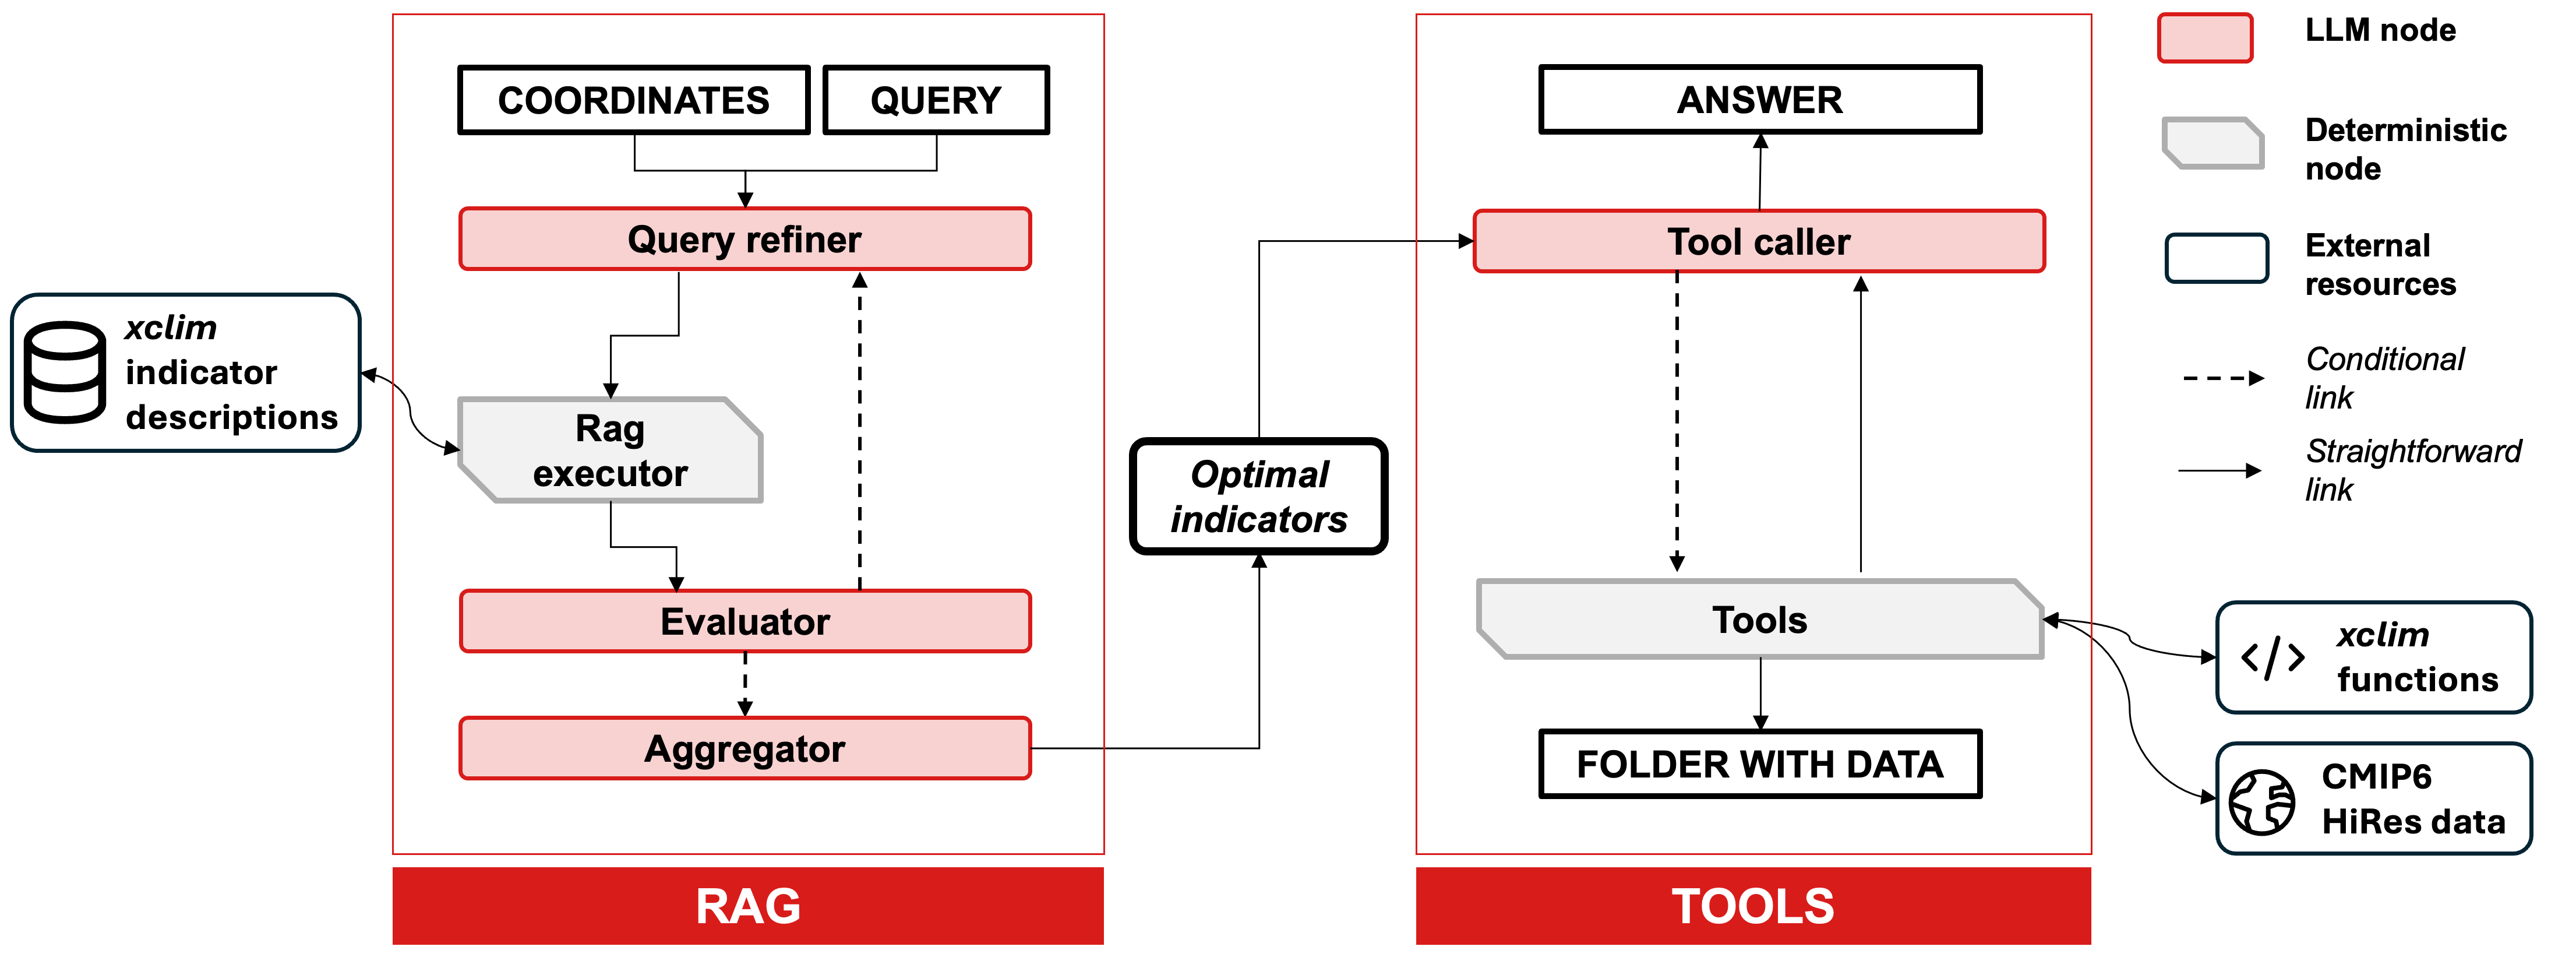
\includegraphics[
            width=\textwidth,
            height=0.34\textheight,
            keepaspectratio
        ]{Chapter5/figs/xclim-architecture.png}
        \caption{Architecture of XCLIM-AI.}
        \label{fig:xclim-architecture-workflow}
    \end{subfigure}

    \vspace{0.5cm}

    \begin{subfigure}{0.9\textwidth}
        \centering
        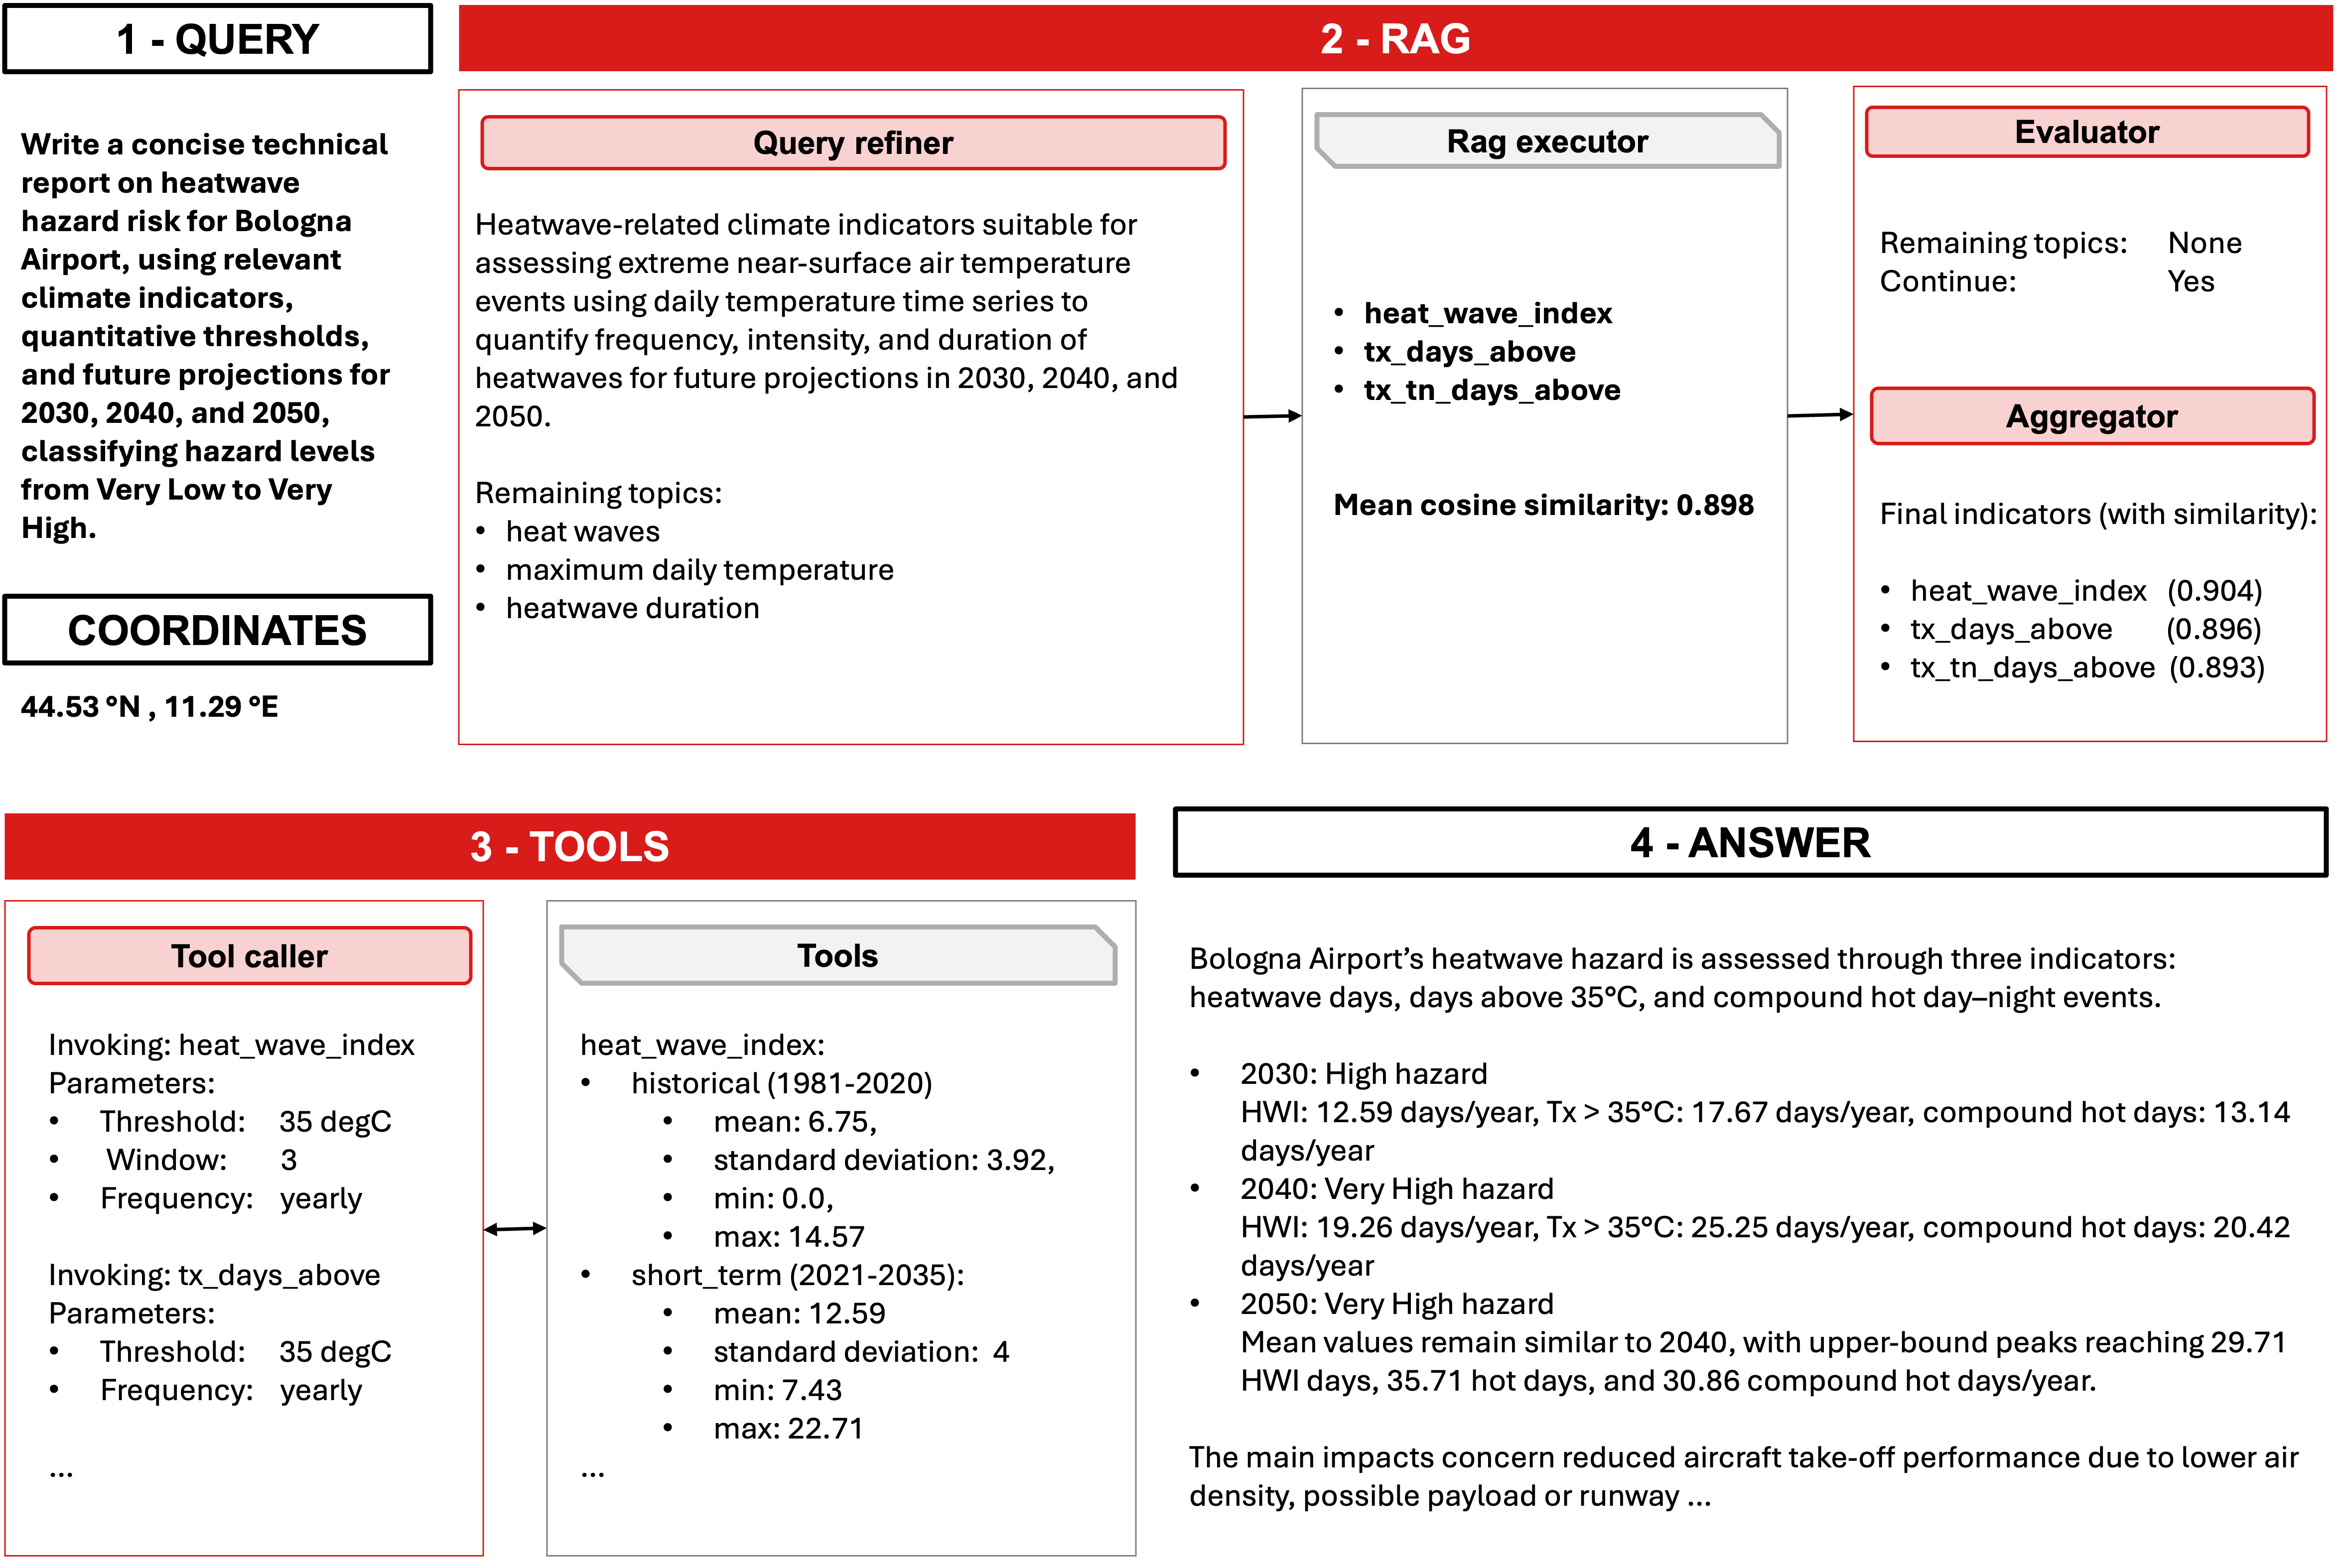
\includegraphics[
            width=\textwidth,
            height=0.34\textheight,
            keepaspectratio
        ]{Chapter5/figs/workflow.png}
        \caption{Example execution of the XCLIM-AI workflow.}
        \label{fig:xclim-architecture-example}
    \end{subfigure}

    \caption{
        Architecture and example execution of the XCLIM-AI workflow. Panel~(a) shows the overall architecture, combining a retrieval module that maps the user query to relevant \emph{xclim} indicators with a tool-calling module that executes the selected indicators on climate data and returns quantitative evidence for response generation. Panel~(b) illustrates an example execution in which the query is refined, matched to candidate indicators through retrieval-augmented generation, evaluated and aggregated, and finally passed to the tool-calling module for indicator computation
        and evidence-grounded answer generation.
    }
    \label{fig:xclim-architecture}
\end{figure}

\clearpage


\subsubsection{XCLIM-AI as a ClimSight Agent} \label{climsight-xclim}

\begin{figure}[H]
    \centering
    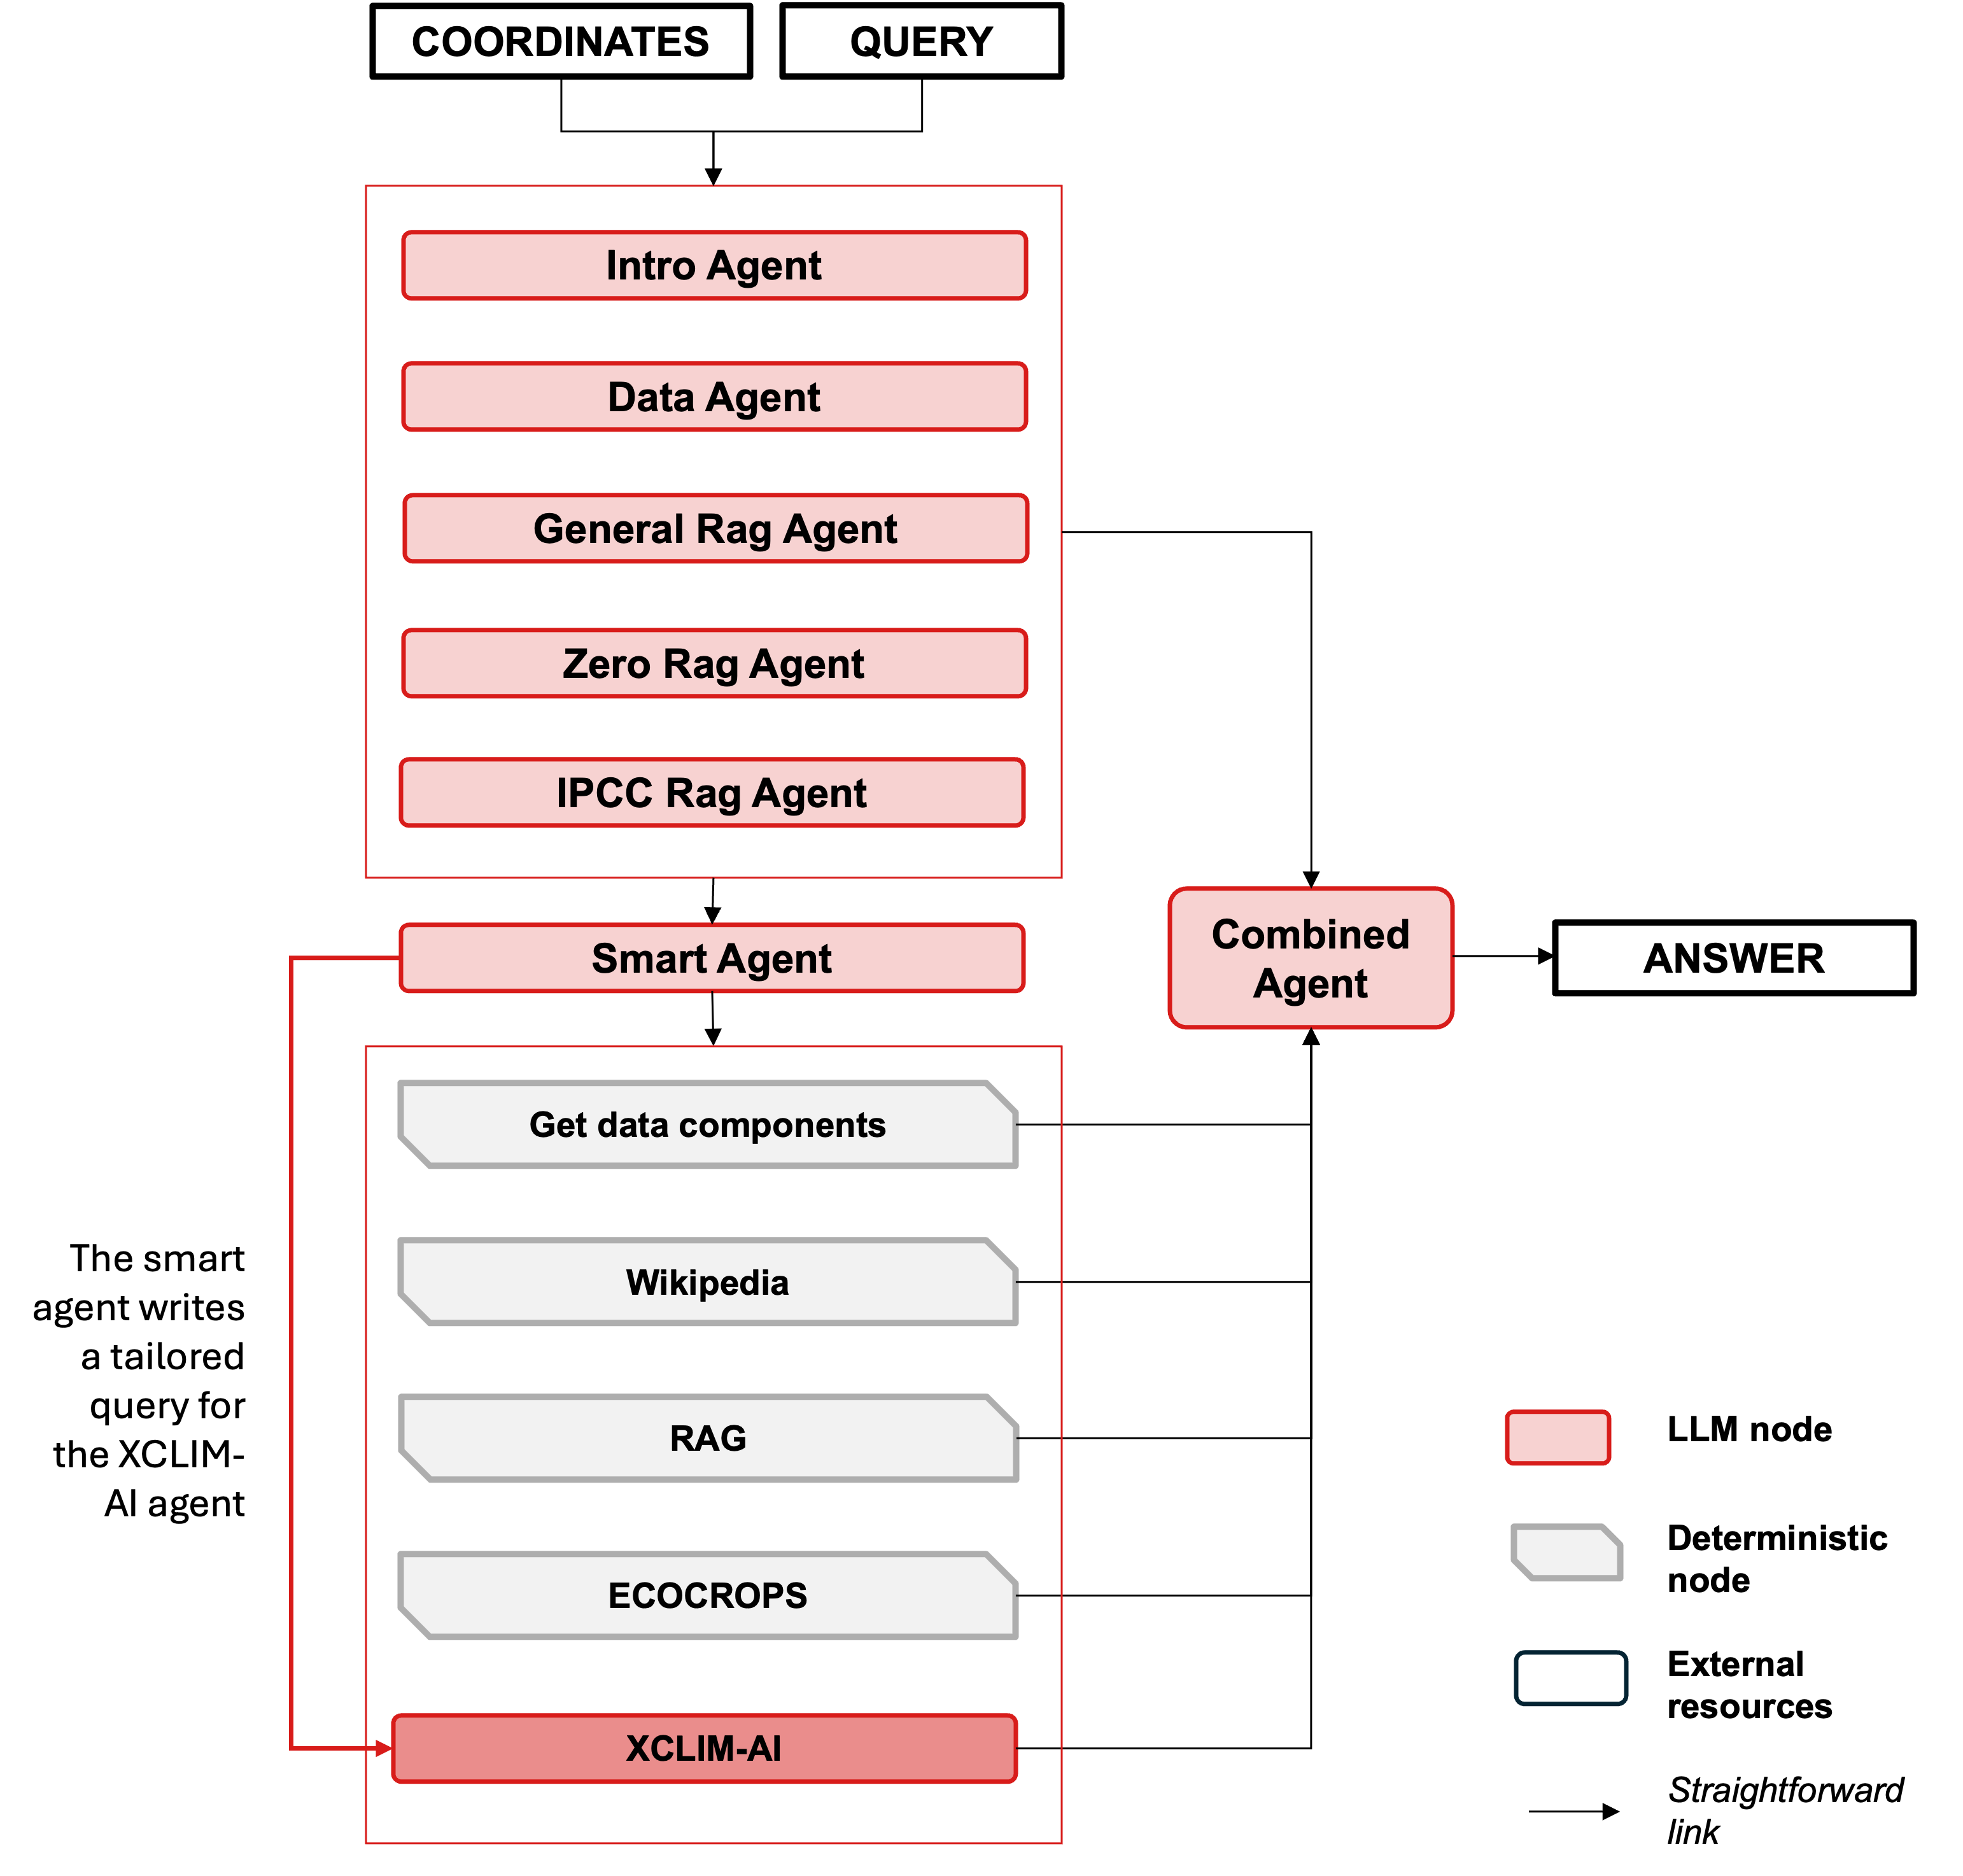
\includegraphics[width=0.75\linewidth]{Chapter5//figs/climsight-augmented.png}
    \caption{
    Architecture of ClimSight-XCLIM. XCLIM-AI is integrated as a callable component of the ClimSight smart agent, which formulates a tailored query for climate-indicator computation after the initial ClimSight agents have contextualized the user request.
    }
    \label{fig:climsight-xclim-architecture}
\end{figure}

ClimSight \citep{koldunov_local_2024, kuznetsov_transforming_2025} is an open-source agentic tool that integrates LLMs with geographical and climate data to provide localized climate information. Its modular design is based on LangGraph \citep{langchain_langgraph_2024} and LangChain \citep{langchain_langchain_2023}, and enables tailored analyses for different application domains while supporting interoperability with other systems.

By default, ClimSight employs five agents for analyzing the query, retrieving climatological data from a kilometer-scale model \citep{rackow_multi-year_2025}, and performing RAG over sectoral literature (Fig.~\ref{fig:climsight-xclim-architecture}). An additional agent, called the smart agent, can access external tools and refine queries for the RAG process.

We deployed XCLIM-AI, in the configuration described in the previous section, as a callable for the smart agent. This means that XCLIM-AI is invoked after ClimSight has already processed a substantial amount of information. Therefore, the smart agent can tailor a query for the XCLIM-AI agent that already incorporates insights from the previous analysis, ideally making the selection and computation of the appropriate climate indicator more efficient.

\subsection{Evaluation Design} \label{methods_evaluation_design}
\subsubsection{Evaluation dimensions} \label{evaluation-dimensions}

We evaluate system outputs along four dimensions: relevance, credibility, uncertainty communication, and actionability. These dimensions were selected because Climate Services requires information to be tailored to the user and decision context, scientifically trustworthy, explicit about limitations and uncertainty, and useful for adaptation planning and action \citep{lemos_narrowing_2012, hewitt_global_2012, vaughan_climate_2014, jahan_assessing_2023, boon_defining_2024, boon_developing_2025}. They also reflect the broader literature on usable knowledge, where the value of scientific information for decision-making is commonly associated with salience, credibility, and legitimacy \citep{cash_knowledge_2003, dilling_creating_2011, mcnie_delivering_2013}.

\paragraph{Relevance.}
Relevance refers to the extent to which the response addresses the user's question, location, sector, and decision context. In Climate Services, information is rarely useful in the abstract: the same climate variable or indicator may have different meanings depending on the asset, exposure, vulnerability, planning horizon, and adaptation problem considered. For this reason, Climate Service evaluation frameworks emphasize the need for information that is tailored to users' needs, problems, and decision-making contexts \citep{vaughan_climate_2014, jahan_assessing_2023, boon_developing_2025}. In the context of LLM-based systems, relevance therefore measures whether the answer moves beyond generic climate statements and selects evidence, indicators, spatial references, and impacts that are appropriate for the specific query.

\paragraph{Credibility.}
Credibility refers to the perceived scientific adequacy, trustworthiness, and evidential grounding of the response. Climate Services are expected to rely on scientifically sound information and expertise, but credibility also depends on whether users can understand why a conclusion should be trusted \citep{hewitt_global_2012, vaughan_climate_2014}. This is particularly important for LLM-based systems, whose responses may be fluent and authoritative while lacking traceable evidence or reproducible analytical support. We therefore assess credibility not only as factual plausibility, but as the degree to which the response is supported by identifiable sources, transparent reasoning, appropriate use of data, and scientifically valid procedures. This criterion is closely related to the literature on usable science, where credibility is one of the core attributes that enables knowledge to inform decisions \citep{cash_knowledge_2003, dilling_creating_2011, mcnie_delivering_2013}.

\paragraph{Uncertainty communication.}
Uncertainty communication refers to the extent to which the response explicitly acknowledges, qualifies, and communicates the limitations of the information provided. Climate information is inherently uncertain because it depends on observational constraints, model structure, internal variability, emission scenarios, downscaling choices, spatial resolution, and indicator definitions. For adaptation decisions, these uncertainties should not simply be omitted or treated as a weakness; rather, they should be communicated in ways that help users interpret the robustness, range, and conditional nature of the evidence \citep{boon_defining_2024, boon_developing_2025}. In our evaluation, this criterion captures whether the answer makes clear what assumptions are involved, and how these uncertainties affect the interpretation of the results.

\paragraph{Actionability.}
Actionability refers to the degree to which the response can support concrete adaptation reasoning, planning, or decision-making. A Climate Service output may be scientifically correct and relevant, yet still have limited practical value if it does not help users understand implications, compare options, identify risks, or frame possible responses. The Climate Services literature increasingly emphasizes that successful services should contribute to better decisions, increased user capacity, and tangible or intangible benefits for adaptation \citep{lemos_narrowing_2012, vaughan_climate_2014, boon_successful_2022, boon_developing_2025}. In the context of LLM-based responses, actionability therefore evaluates whether the answer translates climate evidence into decision-relevant implications, such as adaptation priorities, risk thresholds, affected activities, or planning considerations, while avoiding unsupported prescriptions.

\subsubsection{Evaluation set-up} \label{evaluation-set-up}
These dimensions are evaluated over the answers that different LLM systems give to 50 climate-related questions from \citep{kuznetsov_climsight-gpt41-mini-climate-assesments_2025}. The dataset focuses on localized questions related to climate change adaptation, each categorized into thematic domains. For this evaluation, we randomly sampled questions from ten themes, covering Agriculture, Resource Management, Economics, and Human Health. To generate the answers, we used GPT-4.1 \citep{openai_gpt-41_2025} as model for the Plain-LLM, as well as backbone model for the three other systems. 

To ensure comparability across systems, we defined a standardized output schema that all systems were required to follow when generating responses. 
This schema consisted of four structured sections, each explicitly aligned with the four evaluation dimensions described above, ensuring that all systems provided outputs in a consistent and directly comparable format.

Models were instructed to keep each section clearly separated, to avoid unsupported claims, and to explicitly indicate "N/A" where information was unavailable. This enforced uniform formatting reduced stylistic variability between systems, enabling a fairer evaluation across criteria. A complete example of the generated outputs is provided in Supplementary Material B.

Thus, we evaluated the answers using a dual assessment framework combining both an automated LLM-as-a-judge setup \citep{gu_survey_2025} and a human expert-based evaluation (see Supplementary Material C for statistics about the distribution of evaluators). In both cases, evaluators followed the same pairwise protocol: for each question, they were shown two responses side by side, one from the Plain-LLM baseline and one from one of the other systems, without being informed of which system produced each answer. Evaluators were then tasked with assigning scores on a 1–10 scale across the four evaluation dimensions. The full instruction given to the human and LLM evaluators is reported in Supplementary Material D.

When using LLM as judges, pairwise comparison has been shown to better align with human judgments than direct scoring \citep{liu_aligning_2025}. However, recent findings indicate that such evaluations may introduce biases, such as a preference for verbose or authoritative answers \citep{jeong_comparative_2025, wu_style_2023}, and a position bias, where the first-presented response tends to receive slightly higher scores \citep{shi_judging_2025}. To mitigate these effects, we adopted two strategies: (i) all system outputs were generated following a standardized, rigid structure to minimize stylistic variability (as explained above), and (ii) the order of response presentation was randomized for each evaluation instance, reducing potential positional bias.

It has been widely demonstrated that the outcomes of LLM-as-a-judge evaluations are strongly dependent on the specific model used as evaluator. In particular, LLMs often display a self-preference bias, favoring outputs generated by the same model \citep{wataoka_self-preference_2024}, or by models of similar size and belonging to the same family \citep{li_preference_2025}. At the same time, larger and reasoning models generally provide more reliable evaluations, but they introduce novel sources of bias compared to lighter or more traditional LLMs, such as the recently identified superficial reflection bias \citep{wang_assessing_2025}. To reduce the dependence on the specific choice of the evaluator, we employed an ensemble of 22 LLMs, both proprietary and open-source, spanning different families and sizes (see Supplementary Material E for the specifics of the models).


\section{Results}

This section presents the results of the evaluation procedure. We analyze the $\Delta$ values (Section \ref{relative-scores}), computed as the difference between the system score  and the corresponding Plain-LLM score for each answer and evaluation criteria.  In this formulation, the $\Delta$ values indicate the extent to which each system differs from the baseline, defined as the performance of the Plain-LLM.

Section \ref{agreement} presents the agreement level between the human evaluators and the llm judges employed in the evaluation.



\subsection{Effects of Augmentation on Epistemic Quality} \label{relative-scores}


\begin{figure}[H]
    \centering

    \begin{subfigure}{0.9\textwidth}
        \centering
        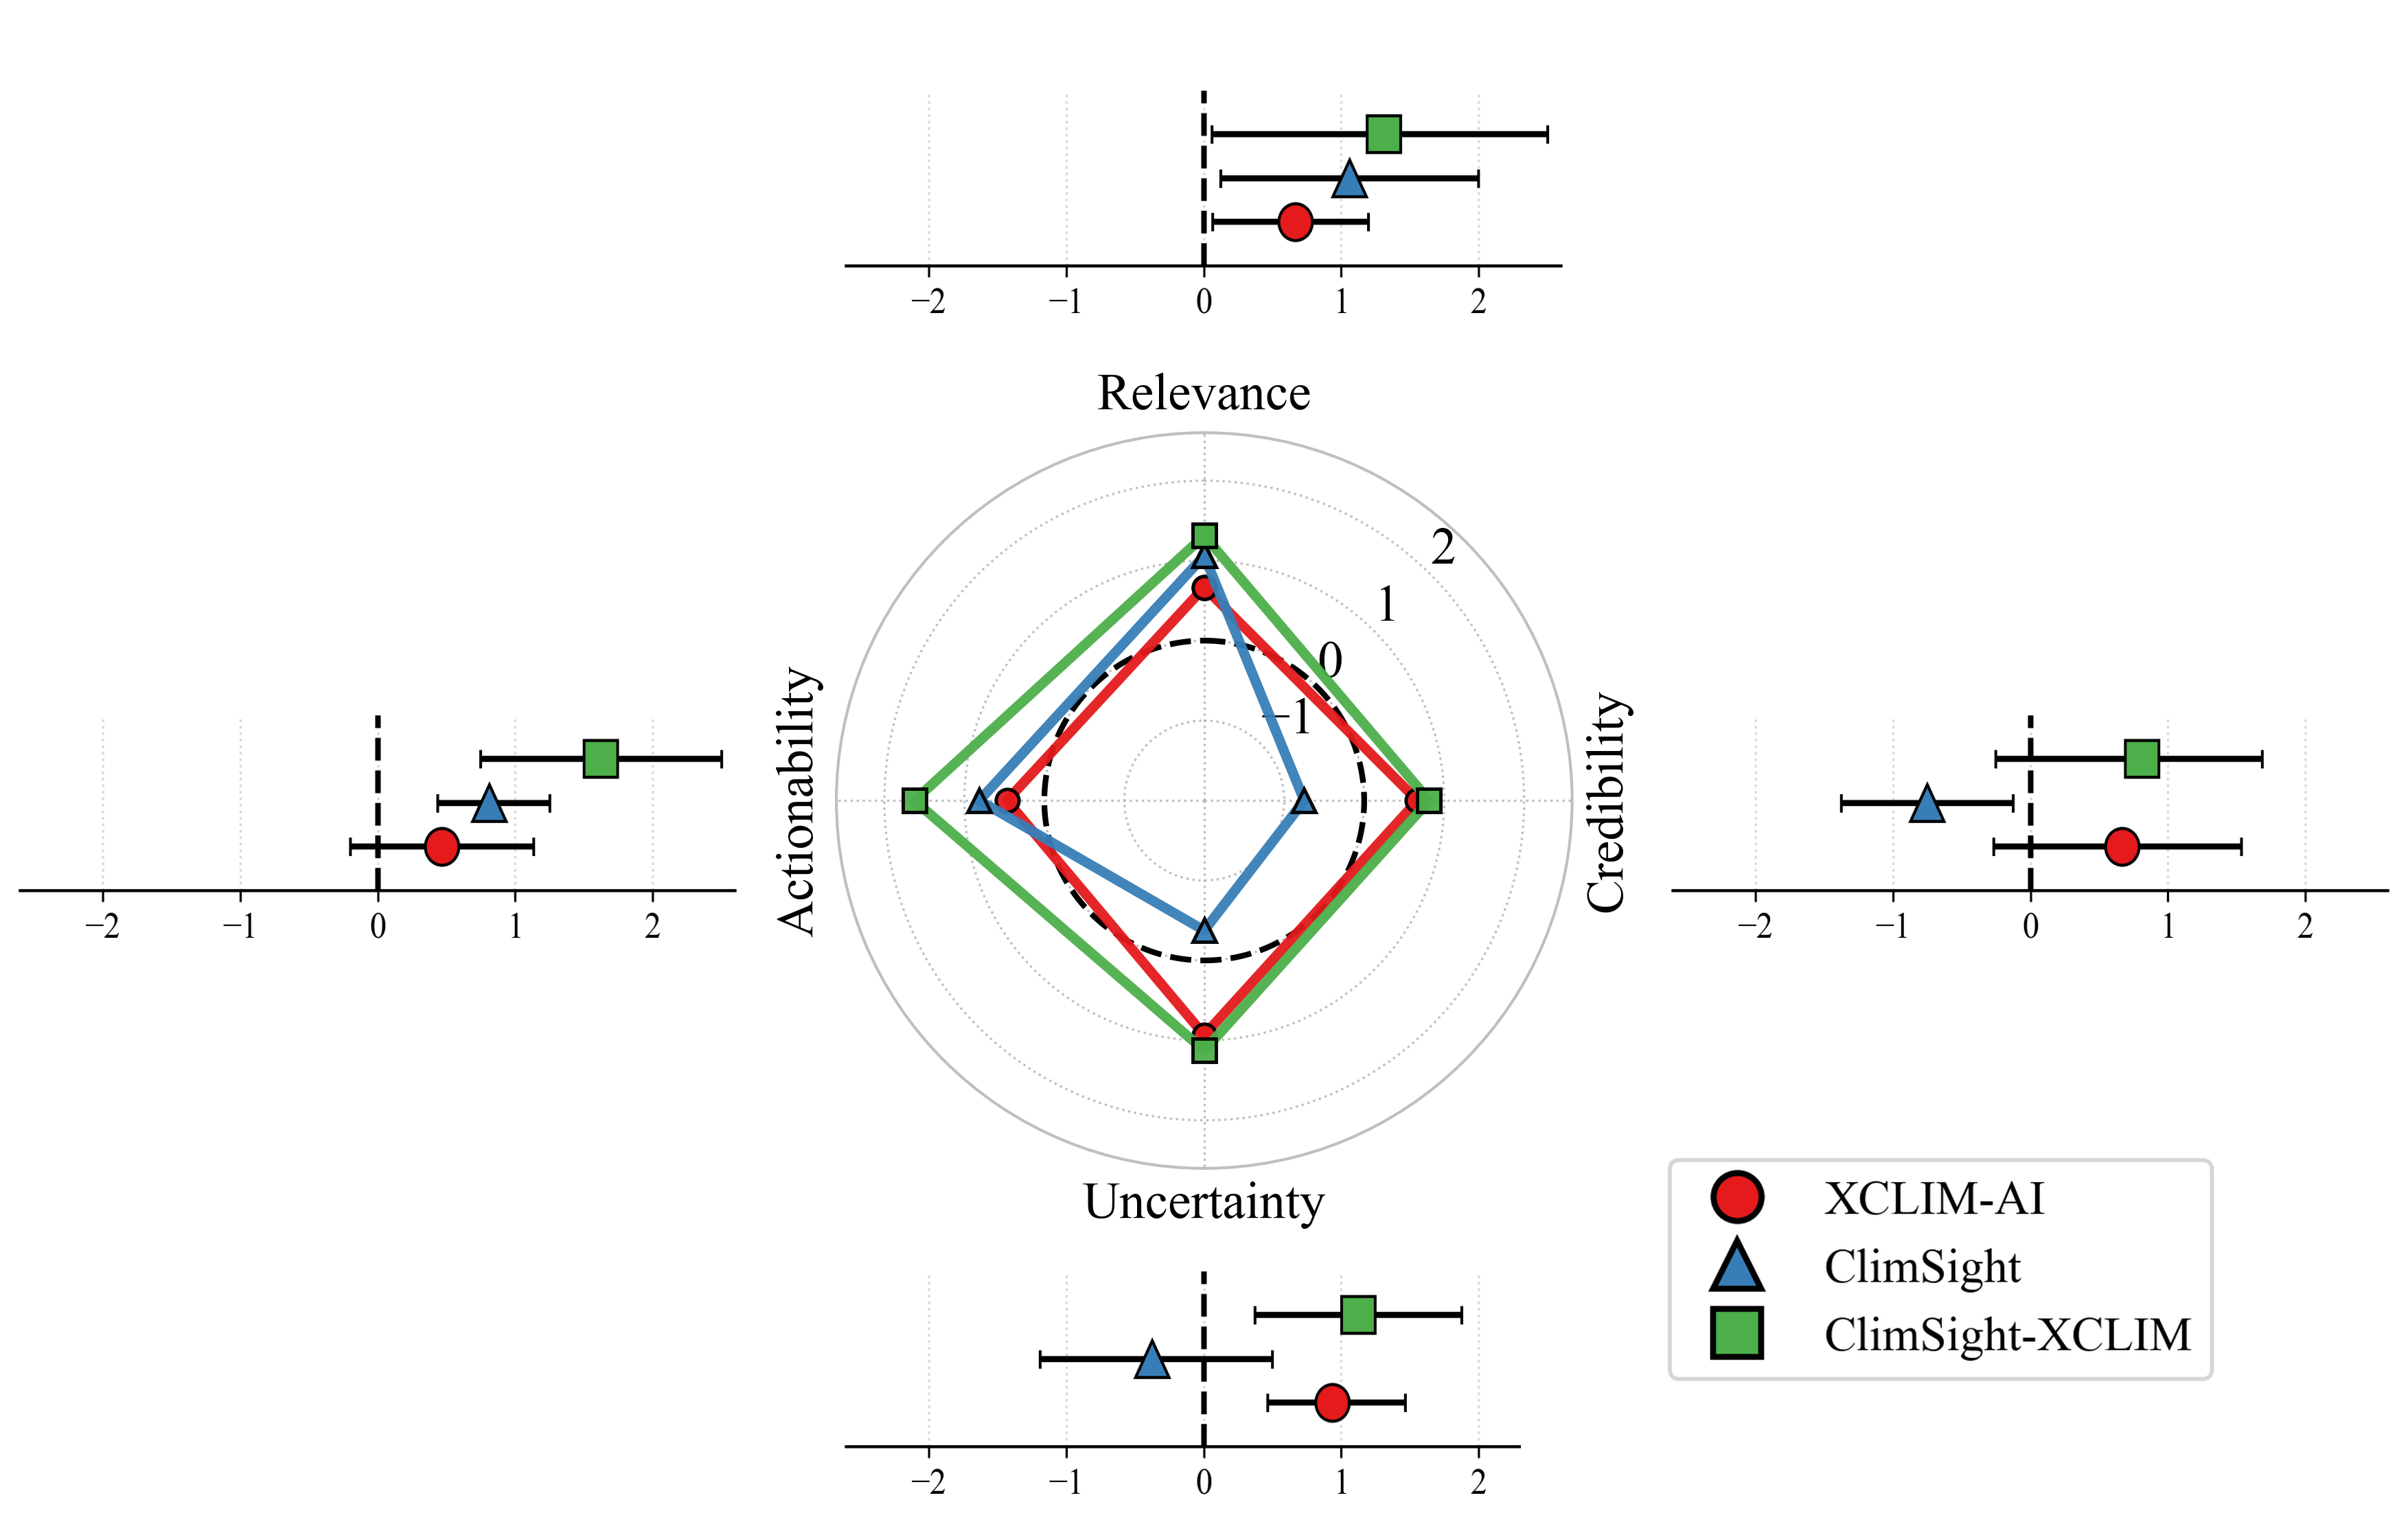
\includegraphics[
            width=\textwidth,
            height=0.34\textheight,
            keepaspectratio
        ]{Chapter5/figs/combined_cardinal_human.png}
        \caption{Human evaluators.}
        \label{fig:combined-human}
    \end{subfigure}

    \vspace{0.5cm}

    \begin{subfigure}{0.9\textwidth}
        \centering
        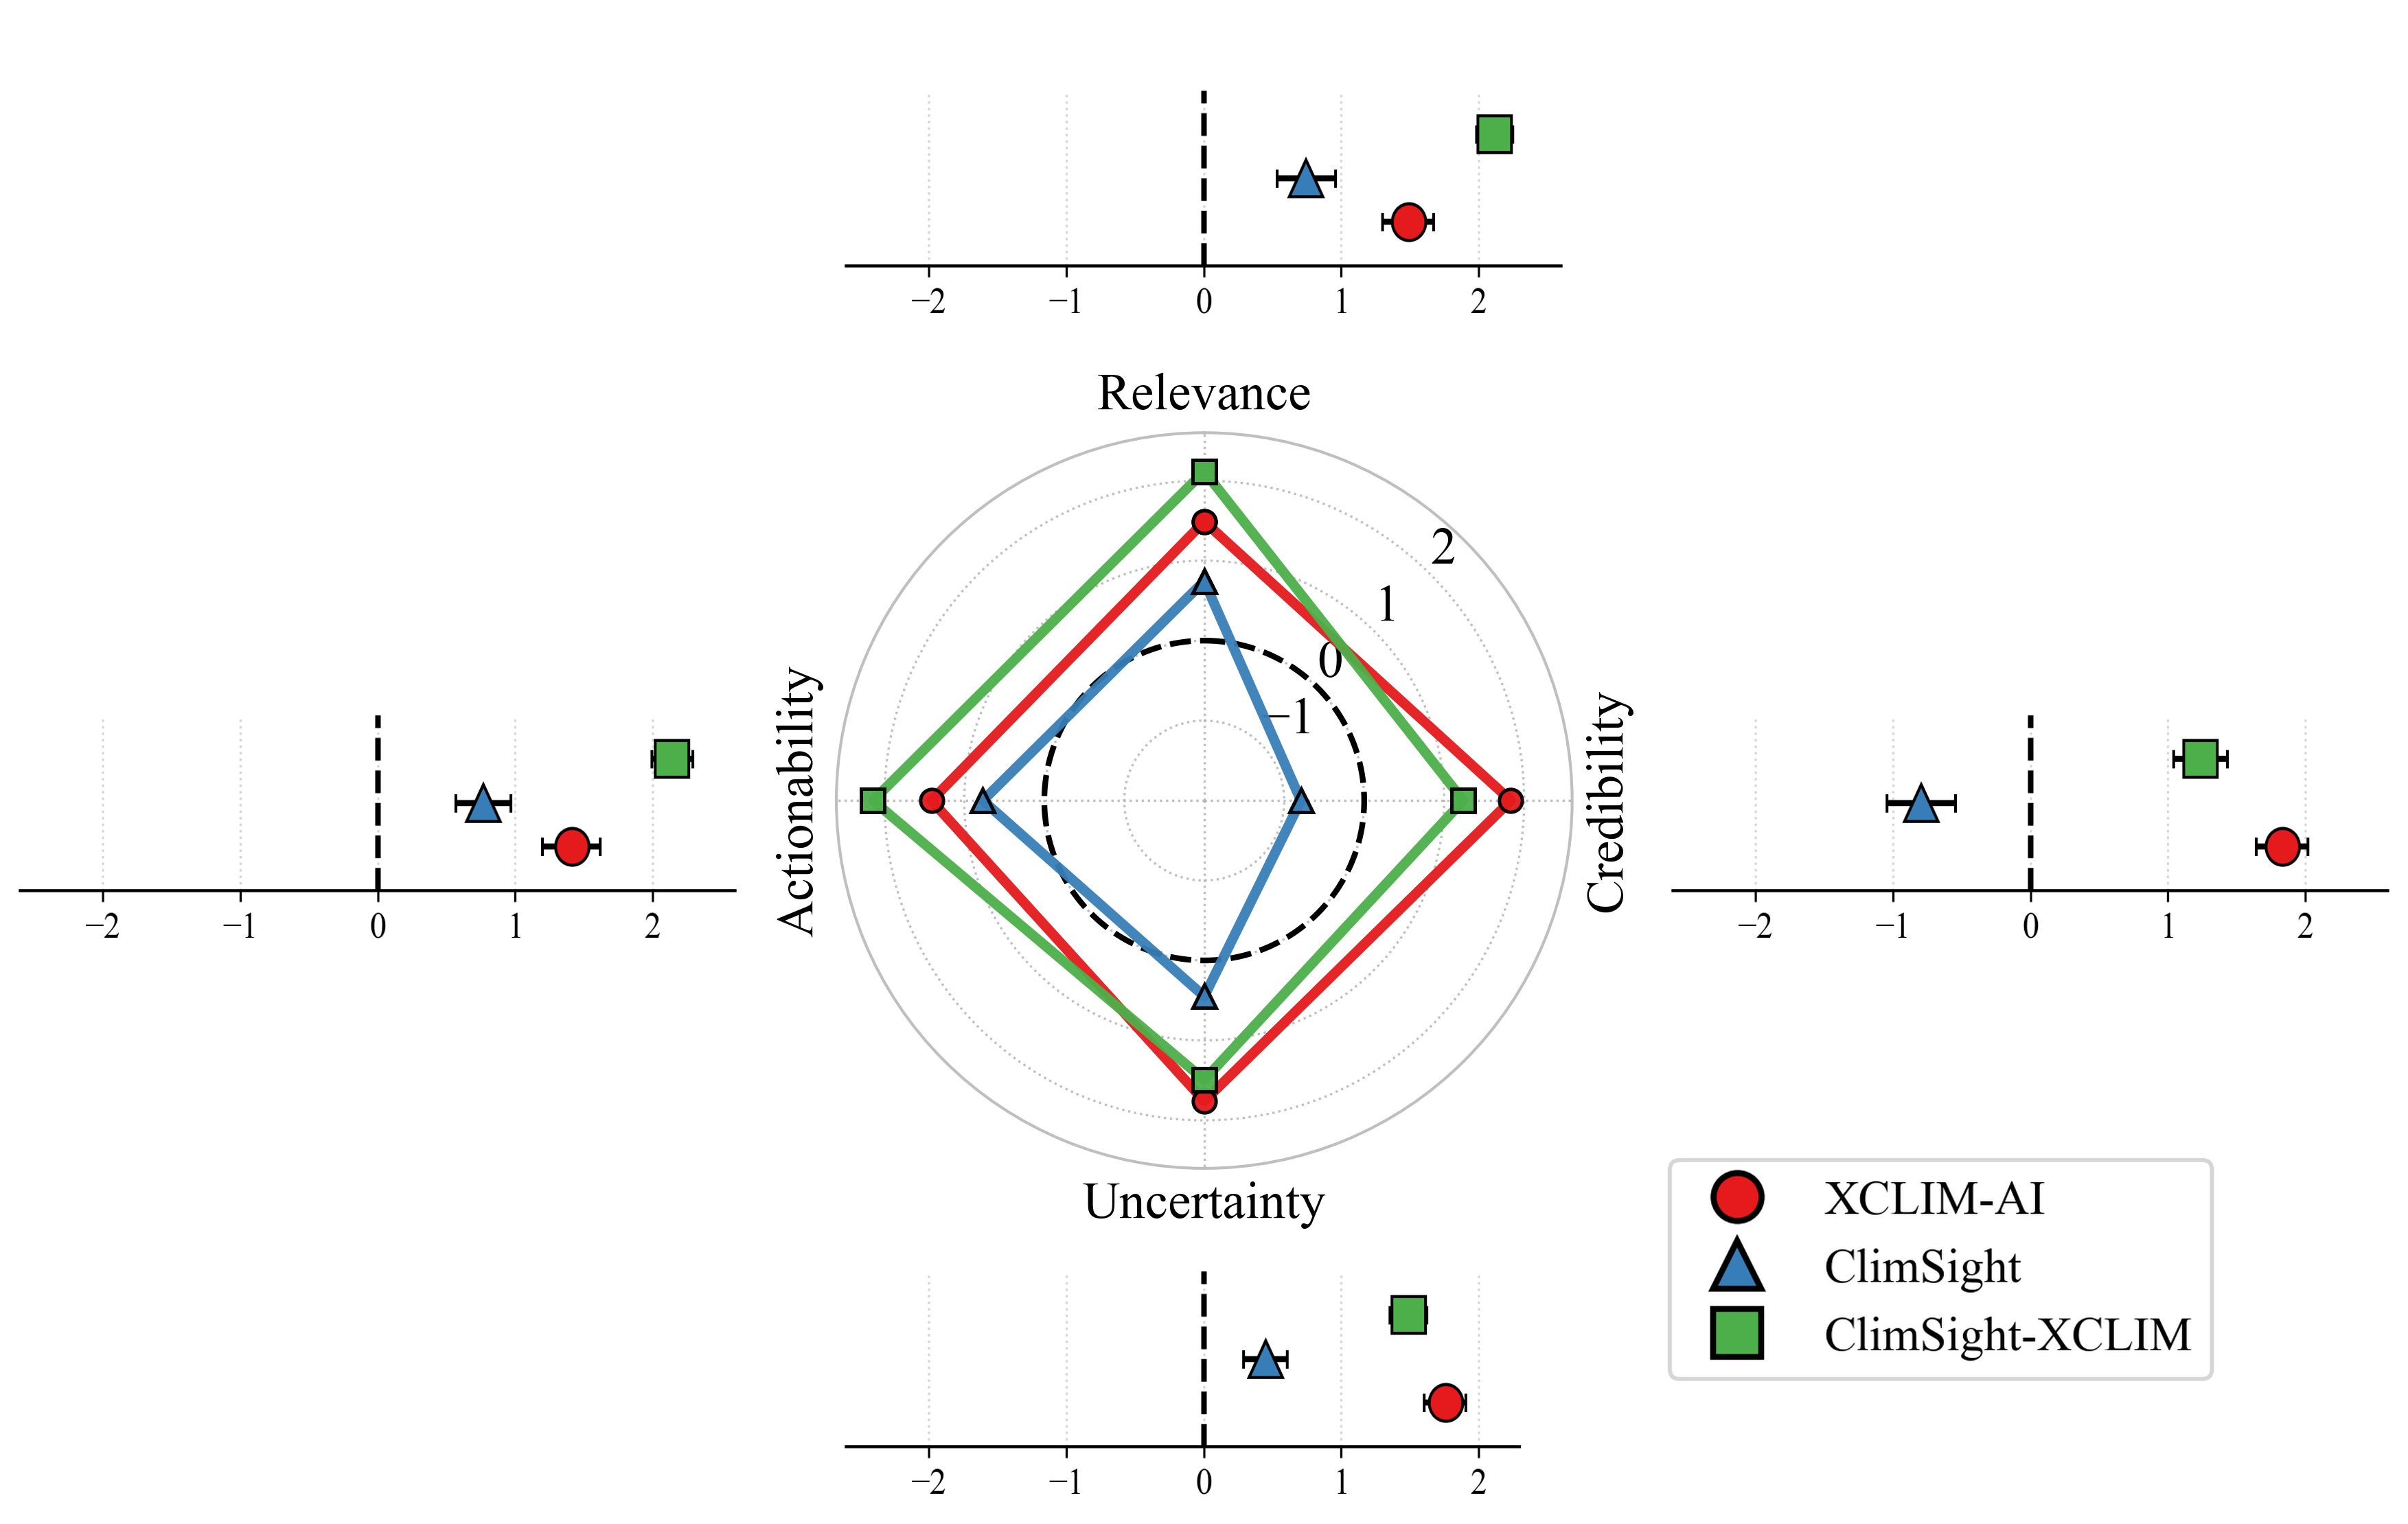
\includegraphics[
            width=\textwidth,
            height=0.34\textheight,
            keepaspectratio
        ]{Chapter5/figs/combined_cardinal_llm.png}
        \caption{LLMs as judges.}
        \label{fig:combined-llm}
    \end{subfigure}

    \caption{
        The central radar plot displays the average scores across all criteria, whereas the four subpanels show 95\% confidence intervals computed via a bootstrap procedure. For each metric we repeatedly drew 10{,}000 new samples from the original data and calculated the mean for each resample; the distribution of these bootstrap means was then used to derive the percentile bounds corresponding to a 95\% confidence level. The dashed line at $\Delta = 0$ highlights the point at which system performance equals that of the Plain-LLM baseline.
    }
    \label{fig:combined-cardinal}
\end{figure}

Figure~\ref{fig:combined-cardinal} report the aggregated scores collected during the evaluation. Human evaluation (Figure~\ref{fig:combined-human}) includes fewer ratings, as each question was assessed by a single expert. In contrast, all 22 LLM judges evaluated every answer (Figure~\ref{fig:combined-llm}), resulting in a much larger number of observations. This naturally leads to narrower 95\% confidence intervals for the LLM-based evaluation. Despite this difference in sample size, the overall patterns observed across the two evaluation methods are broadly consistent.

In both evaluations, all enhanced systems improve over the Plain-LLM baseline in terms of relevance and actionability.
The clearest gains are observed for ClimSight-XCLIM, which achieves the highest increase in actionability according to both human ($+1.6$) and LLM ($+2.1$) judges.
The same system also obtains a similar improvement in relevance, with closely aligned scores from LLM judges ($+2.1$) and human experts ($+1.3$).
Importantly, these effects are consistent: for ClimSight-XCLIM, the confidence intervals remain entirely above zero for both criteria and both evaluation methods.

The other two enhanced systems show a similar pattern, although less pronounced.
XCLIM-AI improves relevance in both evaluations, with median gains of $+0.7$ for human evaluators and $+1.5$ for LLM judges.
Its actionability gain is more clearly captured by the LLM-based evaluation ($+1.4$), while human evaluators assign a smaller increase ($+0.5$).
This latter value represents the only case in relevance and actionability where the confidence interval is not entirely positive, with a lower bound slightly below zero ($-0.2$).
ClimSight, instead, shows balanced improvements across the two criteria: relevance increases by $+1.1$ in the human evaluation and $+0.7$ in the LLM-based evaluation, while actionability improves by $+0.8$ in both cases.
As for ClimSight-XCLIM, all corresponding confidence intervals for ClimSight remain above zero, indicating that these improvements are stable across resampling.

Manual inspection of the generated responses shows that the Plain-LLM tends to produce outputs that are more vague and generic than those of the other systems, whereas the augmented models include more quantitative and context-specific statements, likely increase their perceived quality.

This observation is consistent with recent work on climate-oriented LLMs.
General purpose models can produce fluent and plausible climate explanations, but surface quality does not necessarily guarantee epistemic adequacy, factual grounding, or appropriate communication of uncertainty \citep{bulian_assessing_2024}.
Conversely, approaches that connect LLMs to authoritative climate sources, retrieval systems, and structured climate datasets have been proposed as a way to improve reliability and provide more localized and contextualized responses \citep{vaghefi_chatclimate_2023}.

Our results support this interpretation. The improved relevance and actionability of the enhanced systems appear to derive from their ability to anchor responses in retrievable evidence and computationally derived climate indicators. Notably, ClimSight-XCLIM, which combines both climate information retrieval and indicator computation, is also the system that achieves the highest perceived quality in relevance and actionability.

Our results on uncertainty and credibility highlight substantial disparities across systems. For uncertainty, XCLIM-AI and ClimSight-XCLIM show clear improvements over the Plain-LLM baseline in both evaluation settings.
Human evaluators assign median gains of $+0.9$ to XCLIM-AI and $+1.1$ to ClimSight-XCLIM, while LLM judges assign gains of $+1.8$ and $+1.5$, respectively. By contrast, ClimSight exhibits a weaker and less consistent pattern: human evaluators report a slight decrease in uncertainty expression ($-0.4$) with a lower 95\% confidence value of $-1.25$, whereas LLM judges assign only a small positive change ($+0.4$).

Credibility shows an even sharper separation between systems.
XCLIM-AI improves credibility according to both human evaluators ($+0.7$) and LLM judges ($+1.8$), and ClimSight-XCLIM follows the same positive trend, with gains of $+0.8$ and $+1.2$, respectively.
However, in the human evaluation, the confidence intervals for both XCLIM-AI and ClimSight-XCLIM extend slightly below zero, indicating some uncertainty around the magnitude and stability of these positive effects.
By contrast, the LLM-based evaluation assigns entirely positive confidence intervals to both systems. ClimSight, however, is the only system that deteriorates in credibility across both evaluation methods, with median $\Delta$ scores of $-0.8$ for both human evaluators and LLM judges. This negative effect is stable across resampling, as the confidence intervals remain entirely below zero in both evaluations.

General purpose LLMs can produce coherent and plausible explanations, but they remain prone to hallucination and to weaknesses in factual grounding, specificity, completeness, and uncertainty communication \citep{ji_survey_2023, bulian_assessing_2024}.
This is particularly consequential in climate-related domains, where scientific claims often depend on model uncertainty, scenario assumptions, confidence levels, spatial resolution, and evolving evidence.
In such contexts, credibility depends not only on the fluency of the answer, but also on whether claims can be traced to reliable evidence and to a transparent process of knowledge production.

The credibility results can be interpreted in this light.
The Plain-LLM baseline may appear credible because it can generate fluent explanations and plausible citations ad hoc, even when the evidential basis of specific claims is weak or unverifiable.
Retrieval-based systems such as ClimSight are instead constrained by the sources actually available to them.
When these sources are incomplete, indirect, or insufficiently specific to the user query, the system has fewer opportunities to project unsupported confidence.
As a result, it may appear less credible than the Plain-LLM, not necessarily because it is less grounded, but because its grounding exposes the limits of the available evidence.

This interpretation is consistent with work on attribution in natural language generation, which argues that claims about the external world should be evaluated according to whether they are supported by identifiable sources \citep{rashkin_measuring_2022}.
It is also aligned with climate-oriented QA systems, where grounding LLMs in authoritative sources such as IPCC AR6 has been proposed as a way to reduce hallucination and outdated information while improving the reliability of climate answers \citep{vaghefi_chatclimate_2023}.
However, our results indicate that adding contextual or retrieved information is not, by itself, sufficient to improve credibility.
What matters is also whether the system can make clear how the evidence supports the conclusions it presents.

The stronger performance of XCLIM-AI and ClimSight-XCLIM suggests that climate indicator computation adds a different form of grounding.
In these systems, part of the answer is supported by indicators computed from climate model data through an explicit analytical workflow.
The resulting claims are therefore not only textually grounded, but procedurally grounded: they are connected to indicator definitions, parameter choices, model data, and deterministic calculations.
This provides a stronger basis for quantitative statements and helps explain why XCLIM-AI-based systems improve both perceived credibility and uncertainty communication, while ClimSight improves relevance and actionability but not credibility to the same extent.

\subsection{Agreement Between Human and LLM Evaluators} \label{agreement}

\begin{figure}[H]
    \centering
    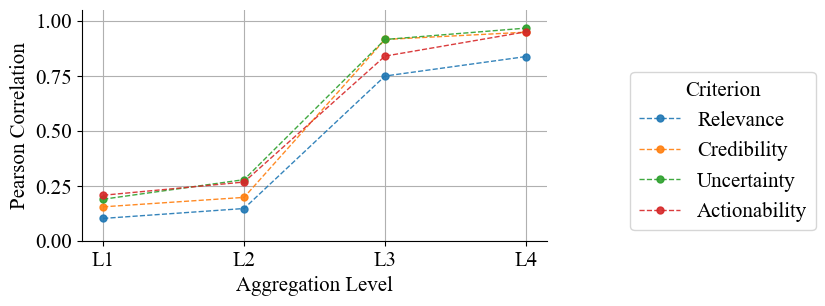
\includegraphics[width=1\textwidth]{Chapter5//figs/icc_evolution.png}
    \caption{
        Human--LLM agreement across increasing levels of aggregation. Pearson correlations are computed between human and LLM-assigned $\Delta$-scores for each evaluation criterion. L1 compares individual human judgments with single-LLM judgments at the question level; L2 averages LLM judgments across judges while preserving question-level comparisons; L3 aggregates scores at the system level for each individual LLM judge; and L4 compares system-level averages after aggregating across both questions and LLM judges.
        }

    \label{fig:icc-levels}
\end{figure}

Our evaluation framework employs 22 LLMs as judges and was designed to reduce judge-specific bias while producing meaningful comparisons with human assessments. In this section, we quantify the agreement between the $\Delta$-scores assigned by the ensemble of LLM judges and those assigned by human evaluators. To this end, we compute the Pearson correlation coefficient between human and LLM-assigned scores at four different levels of aggregation (Figure~\ref{fig:icc-levels}):

\begin{enumerate}
    \item \textbf{Level 1 (L1): Question-level, single-LLM agreement.}
    At this level, each human judgment is compared directly with the score assigned by a single LLM judge on the same question and system.
    No aggregation is performed: every comparison involves one human score and one single-LLM score for each question–system pair.
    Agreement is low across all criteria due to strong item-level variability and judge-specific noise.

    \item \textbf{Level 2 (L2): Question-level, mean-LLM agreement.}  
    This level still operates at the question level, but LLM judgments are aggregated before comparison.  
    For each question–system pair, we compute the average score assigned by all LLM judges, and we compare this mean-LLM score with the corresponding human score.  
    This reduces variability across judges while preserving question-level resolution.  
    Agreement improves moderately.
    
    \item \textbf{Level 3 (L3): System-level, single-LLM agreement.}  
    At this level, we aggregate across questions instead of across judges.  
    For each system, we compute the average human score over all its questions, and we separately compute the average score assigned by each single LLM judge across the same questions.  
    These system-level averages are then compared.  
    Removing item-level noise leads to a sharp increase in agreement.
    
    \item \textbf{Level 4 (L4): System-level, mean-LLM agreement.}  
    This is the most aggregated setting.  
    For each system, we compare the human average across all questions with the average score assigned by all LLM judges, also aggregated across all questions.  
    This combines both forms of aggregation—across judges and across items—and yields the highest agreement across all criteria.
\end{enumerate}

These results show that removing question-to-question variability substantially increases the alignment between LLM judges and human evaluators.
Once scores are aggregated at the system level, even a single-LLM judge already provides a reliable approximation of human assessments.
When the mean-LLM score is used, the agreement becomes remarkably high, with Pearson correlations above 0.95 for all criteria (except relevance, which still exhibits a strong correlation of 0.84).
It should be noted, however, that removing question-level variability implies that the agreement is measured over differences between system-level performance profiles rather than over individual questions.

Overall, these findings suggest that LLM-as-a-judge is highly effective when evaluations are aggregated over multiple items, as aggregation cancels out the substantial noise present in single-question judgments.
However, at the level of individual questions, single-LLM judgments remain unreliable, and their use should therefore be restricted to settings where either ensembles (mean-LLM) or item-level aggregation are feasible.

\section{Discussion}

The results of this chapter address two related questions: how different forms of augmentation change the contribution of LLMs to Climate Services, and how these changes can be evaluated. The main conclusion is that augmentation does not improve all dimensions of epistemic quality equally. Contextual augmentation primarily increases the specificity and practical orientation of responses, whereas computational augmentation provides a stronger basis for quantitative claims. Their combination produces the most consistent improvements, although its effectiveness remains dependent on how the different sources of evidence are integrated within the system architecture. The transition from climate information to knowledge therefore depends not simply on how much information is supplied to the model, but on how that information is produced, connected, and communicated.

The most distinctive contribution of computational augmentation can be described as \emph{procedural grounding}. Textual grounding connects a statement to an identifiable source; procedural grounding additionally connects a quantitative claim to the data, indicator definition, parameters, and analytical procedure through which it was obtained. This establishes a clearer boundary between computed evidence and model inference. 

Nevertheless, computation alone does not transform information into knowledge. A climate indicator becomes meaningful only when interpreted in relation to the exposed system and the decision under consideration. An earlier last spring frost may appear favourable for vineyards, but concurrent changes in budburst can preserve or increase frost vulnerability. Similarly, a projected change in precipitation extremes cannot by itself determine the additional capacity required for an urban drainage system. Procedural and contextual grounding are therefore complementary: the former produces traceable climate information, while the latter connects it to impacts, vulnerabilities, and possible responses.

These observations also demonstrate why conventional evaluations of LLMs are insufficient for Climate Services. Factual correctness and linguistic fluency remain important, but they do not establish whether a response is usable within a specific decision context. An answer may be plausible but geographically irrelevant, quantitatively precise but poorly justified, or scientifically grounded without providing a meaningful interpretation for the user. The four dimensions adopted in this chapter (relevance, credibility, uncertainty communication, and actionability) make these differences explicit and capture complementary attributes of usable climate knowledge. Since different forms of augmentation affect these dimensions in different ways, the same criteria can also inform system design: credibility requires traceable evidence and transparent analytical choices; uncertainty communication requires assumptions, model spread, scenarios, and data limitations to be preserved; and relevance and actionability require climate information to be interpreted in relation to the user's context and decision problem.

The comparison between human and automated evaluations provides a further methodological insight. LLM judges reproduce the overall direction of human assessments reasonably well when their scores are aggregated across questions and evaluators. They can therefore support the comparison of alternative architectures or augmentation strategies during system development. Their agreement with human evaluators is substantially weaker for individual responses, however, and aggregation cannot demonstrate that a judge has correctly assessed the suitability of a specific indicator or recommendation. LLM-based evaluation should therefore be treated as a system-level development instrument rather than as a mechanism for certifying individual Climate Service outputs.

From an operational perspective, systems such as XCLIM-AI can reduce the technical distance between questions expressed in operational language and the indicators, datasets, and procedures required to address them. They could support indicator exploration, preliminary climate risk assessments, comparisons between historical and future conditions, and the preparation of technical reports. They may also facilitate communication between scientists and users by translating practical questions into formal analyses and numerical outputs into accessible explanations.

Several limitations condition these conclusions. The evaluation is based on 50 localized adaptation questions covering ten thematic categories and cannot represent the full diversity of Climate Services. In addition, GPT-4.1 was used as the backbone of all four systems. This choice isolates the contribution of augmentation, but limits the generalizability of the results to models with different tool-use and reasoning capabilities. The XCLIM-AI implementation also represents only one configuration of computational augmentation, constrained by the indicators available in \emph{xclim}, the variables accessible through Open-Meteo, seven HighResMIP models, a selected scenario and set of time periods, and point-based spatial extraction. Operational applications may require observations, additional scenarios, downscaled projections, impact models, and spatial aggregation.

The study evaluates the final responses without independently scoring every component of the analytical chain. It is therefore not always possible to determine whether a weakness originates from indicator retrieval, parameter selection, tool execution, numerical interpretation, or final synthesis. Moreover, the framework measures perceived epistemic quality rather than providing complete verification of scientific correctness. Each question was evaluated by one human expert, while the LLM judges are neither statistically nor epistemically independent. Finally, the experiment concerns fully automated workflows and assesses actionability as a property of the generated text, rather than through its effects on actual decisions. Future work should combine end-to-end evaluation with component-level validation and examine these systems within collaborative Climate Service processes.
\chapter{Discussion}

The studies presented in this dissertation examine different contributions of AI to the Climate Services value chain. Their findings raise three central questions: whether high average performance translates into reliability under specific local conditions; how optimization objectives relate to scientific and operational requirements; and whether AI can provide a reliable interface to external climate knowledge. These questions concern not only the capabilities of individual models, but also the conditions under which their outputs can support Climate Services.

\section{Average Skill and Local Reliability}

Several results reveal a distinction between reproducing broad climatic regularities and representing the departures from those regularities that matter locally. This is particularly evident in the LLM climate-change experiment. The models reproduce an approximately plausible mean warming, but the spatial correlations between the warming fields generated by GPT-5 and Mistral Small 3.1 24B and the ERA5 reference remain below 0.10. Their estimates therefore contain substantially less useful geographical information than their plausible average values might suggest.

The weather-model experiments reveal a related, although distinct, problem. Models initialized from EERIE-AMIP initially move towards an ERA5-like global mean, while retaining regional differences that are not apparent in the global average. This adjustment should not be equated with the compression of spatial variability observed in the LLM estimates. Nevertheless, it raises a similar question about the ability to preserve conditions that differ from the regularities represented during training. Closer agreement with a training reference does not, by itself, demonstrate preservation of the climate state supplied at initialization.

These behaviours motivate a broader question: \emph{are models optimized for high average performance also reliable under the highly specific conditions that matter to Climate Services?} Training objectives determine which errors receive greater weight, while the training data determine which conditions are represented. For deterministic predictions, squared-error minimization favours the conditional mean, potentially smoothing uncertain features. Other objectives and architectures behave differently, and the experiments presented here do not establish a common causal mechanism across models. They do, however, show why aggregate performance is insufficient evidence of local reliability.

This distinction is consequential when information is used near an operational threshold. An error that contributes little to a global score may change whether a condition is classified as hazardous at a particular location. Evaluation should therefore examine the geographical distribution, seasonality, and conditional structure of errors, rather than treating local applicability as a consequence of good average skill.

\section{From Metric Optimization to Scientific Relevance}

A second issue concerns the relationship between what an algorithm optimizes and what a Climate Service needs. A performance metric formalizes a criterion of success, but its improvement has scientific value only insofar as that criterion represents the intended task. Contextual relevance is not automatically contained in an optimization objective; it must be introduced through problem formulation, data selection, methodological choices, and evaluation.

The seasonal framework illustrates this distinction. The algorithm does not independently determine what a meteorological season should mean. The input variables, normalization, temporal processing, and number of classes establish an operational representation of the concept. Its scientific interpretation is then assessed against climatological knowledge and recognizable seasonal behaviour. Machine Learning makes this representation computable and transferable, but does not remove the assumptions through which it was constructed.

Consequently, the projected lengthening of the monsoon describes increased persistence of the multivariate conditions associated with the learned seasonal class. It does not automatically imply greater rainfall totals, improved water availability, or a longer agricultural growing season. These interpretations require additional evidence. The relevant question is therefore not simply whether classification performance improves, but whether the resulting information represents the phenomenon required by the application.

Human expertise is fundamental at this stage, before any final output is reviewed. It determines which distinctions are scientifically meaningful and which conclusions an analysis can support. Automation can reduce the effort required to implement these choices, but cannot establish their contextual appropriateness through optimization alone. Expert involvement should therefore be understood as part of the design of AI-assisted Climate Services, rather than only as a safeguard against occasional model failures.

\section{AI as an Interface to Scientific Knowledge}

The limitations of parametric climate recall suggest a different role for language models: mediating access to scientific evidence rather than substituting for its sources. In this configuration, datasets, publications, and analytical software provide the evidential basis, while the model supports question interpretation, information selection, analysis configuration, and communication.

The evaluation problem consequently changes. It concerns how faithfully the system retrieves, transforms, and communicates the information available to it. Relevant questions include whether the selected evidence addresses the user request, whether computational parameters preserve its intended meaning, and whether the final response distinguishes calculated results from interpretation. An answer can contain correct numerical values while misrepresenting their implications.

The augmentation experiments show that these capabilities depend on system design. Contextual augmentation improves specificity and practical orientation without consistently improving perceived credibility or uncertainty communication. Systems incorporating indicator computation show more consistent gains across the evaluated dimensions. This supports the contribution of \emph{procedural grounding}, through which quantitative statements become associated with explicit data, indicator definitions, parameters, and calculations.

Procedural grounding nevertheless establishes traceability, not automatic appropriateness. A reproducible calculation may use an unsuitable threshold, and a correctly computed indicator may not justify a particular adaptation recommendation. The scientific quality of the interface therefore depends both on preserving the evidence it receives and on respecting the limits of the conclusions that evidence supports.

\section{From Output Quality to Decision Support}

The distinction between a better response and a better decision remains unresolved by the experiments presented here. Higher relevance, credibility, or actionability scores indicate improvements according to the adopted evaluation criteria; they do not demonstrate that users make more effective adaptation decisions. Similarly, stronger agreement between human and LLM evaluators after aggregation supports comparative assessment within the tested systems, but does not certify individual recommendations.

Operational evaluation should therefore distinguish analytical correctness, communication quality, and practical usefulness. These dimensions require complementary evidence. Component-level checks can identify errors in data selection or computation, while collaborative evaluations with providers and users are needed to assess whether the information addresses an actual decision problem. Such evaluations should also examine whether explicit uncertainty and appropriate qualification help users interpret results, rather than rewarding confidence independently of its evidential basis.

\section{Scope and Evolution of the Proposed Frameworks}

The findings concern selected models, configurations, variables, and applications. They should not be interpreted as immutable limitations of AI or as evidence that all architectures exhibit the same behaviour. In particular, the weather-model analysis remains an initial assessment, while the knowledge-oriented experiments do not constitute validation of a complete operational Climate Service.

The frameworks developed here seek to separate scientific requirements from specific implementations, making their approach as model-agnostic as possible. This independence is necessarily partial. New training objectives, architectures, and analytical capabilities may alter existing failure modes and introduce others that the present benchmarks do not capture. Evaluation methods must therefore remain open to revision: a framework that is appropriate for current systems may be insufficient for future developments.

The more durable contribution lies in identifying what must be examined: performance under relevant conditions, the scientific meaning of optimized objectives, traceability of evidence, and the validity of its interpretation. These requirements provide a basis for integrating evolving AI capabilities into Climate Services while retaining scrutiny of the assumptions and judgments on which their usefulness depends.

% ******************************************************************************
% ******************************** Bibliography *******************************

% The bibliography databases are declared in Preamble/preamble.tex with:
%
% \addbibresource{References/references_chapter_1.bib}
% \addbibresource{References/references_chapter_3.bib}
%
% Do not use \bibliography or \bibliographystyle with biblatex.

\cleardoublepage

\begin{spacing}{0.9}

    \printbibliography[
        heading=bibintoc,
        title={References}
    ]

\end{spacing}


% ******************************************************************************
% ******************************** Appendices *********************************

\begin{appendices}

    % ******************************* Thesis Appendix A ****************************
\chapter{Appendix} 
\label{Appendix1}

    % % ******************************* Thesis Appendix B ********************************

\chapter{title of appendix}





\end{appendices}


% ******************************************************************************
% *********************************** Index ************************************

\printthesisindex


% ******************************************************************************
% ****************************** Acknowledgements ******************************

% ************************** Thesis Acknowledgements **************************

\begin{acknowledgements}      


And I would like to acknowledge ...


\end{acknowledgements}



% ******************************************************************************
% ******************************** End Document *******************************

\end{document}